%!TEX root = dgplvm.tex
\newlength\figureheight
\newlength\figurewidth

\section{Experiments}

\subsection{Experiments on Dimensionality Reduction}
\begin{frame}{Oil dataset}
    \begin{minipage}{.48\textwidth}
        It is dataset modeling non-intrusive measurements on a oil. The flow in the pipe can be \textbf{horizontally stratified}, \textbf{nested annular} or \textbf{homogeneous}. The data lives in a 12-dimensional measurement space, but is known to live on a reduced dimensionality.
    \end{minipage}
    \begin{minipage}{.48\textwidth}
        \begin{figure}
            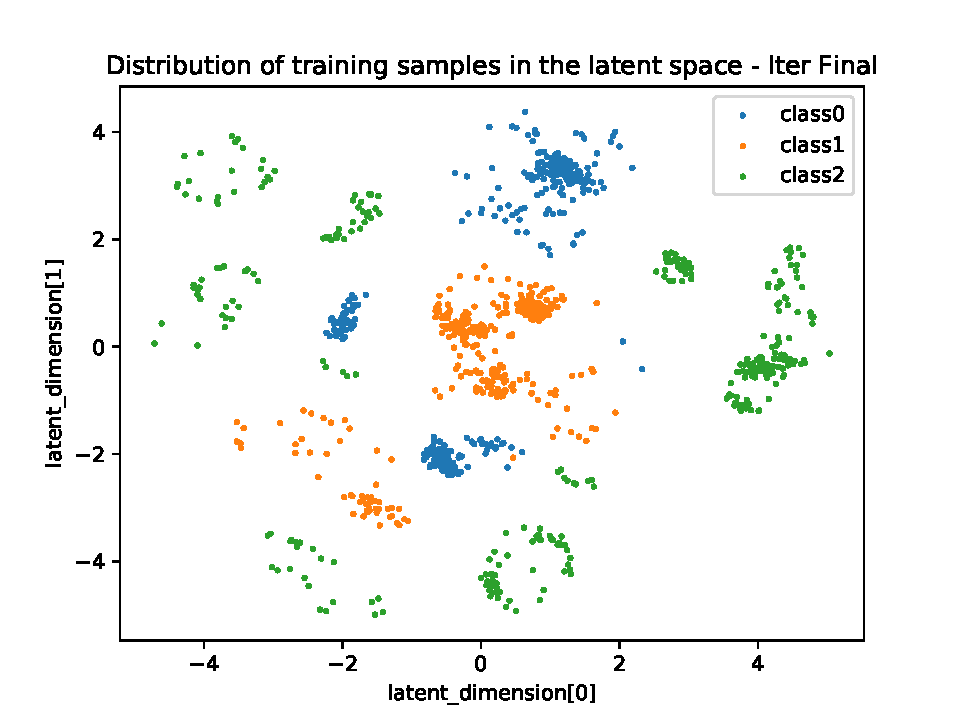
\includegraphics[width=\textwidth]{oil_dim2.pdf}
        \end{figure}
    \end{minipage}
\end{frame}

%\begin{frame}{Experiment on number of hidden layers}
%    \setlength\figureheight{.5\textheight}
%    \setlength\figurewidth{\textwidth}
%    % This file was created by matplotlib2tikz v0.6.11.
\begin{tikzpicture}

\definecolor{color1}{rgb}{0.545098039215686,0.564705882352941,0.619607843137255}
\definecolor{color0}{rgb}{0.898039215686275,0.898039215686275,0.968627450980392}
\definecolor{color3}{rgb}{0.513725490196078,0.658823529411765,0.231372549019608}
\definecolor{color2}{rgb}{0.207843137254902,0.447058823529412,0.776470588235294}
\definecolor{color4}{rgb}{0.768627450980392,0.305882352941176,0.32156862745098}

\begin{axis}[
xlabel={Time},
ylabel={RMSE},
xmin=0.837, xmax=389.006,
ymin=-0.018205, ymax=1.209505,
width=\figurewidth,
height=\figureheight,
tick align=outside,
tick pos=left,
xmajorgrids,
x grid style={color0},
ymajorgrids,
y grid style={color0},
axis line style={color1},
legend style={draw=white!80.0!black},
legend cell align={left},
legend entries={{0 HL},{1 HL},{2 HL}}
]
\addplot [semithick, color2]
table {%
0.837 0.8273
1.446 0.8117
2.072 0.7788
2.717 0.6751
3.262 0.6185
4.207 0.7072
4.73 0.6148
5.756 0.5561
6.332 0.547
7.081 0.5248
7.612 0.4333
8.12 0.5266
8.626 0.4458
9.132 0.4732
9.61 0.4246
10.109 0.4032
10.619 0.4033
11.123 0.3886
11.611 0.3591
12.125 0.3452
12.633 0.3279
13.123 0.349
13.637 0.3196
14.141 0.3073
14.643 0.3138
15.529 0.316
16.203 0.2831
16.86 0.287
17.486 0.2929
18.277 0.2669
18.764 0.2251
19.603 0.245
20.137 0.2511
20.778 0.2404
21.388 0.235
22.041 0.2499
22.657 0.2355
23.26 0.2274
23.86 0.2418
24.482 0.2041
25.174 0.2329
26.128 0.2157
26.665 0.217
27.341 0.2045
27.998 0.227
28.65 0.2115
29.284 0.2031
29.863 0.2064
30.497 0.2111
31.132 0.2027
31.764 0.2174
32.698 0.1873
33.566 0.1865
34.556 0.2224
35.161 0.1854
35.759 0.1973
36.386 0.18
37.021 0.1768
37.619 0.1812
38.234 0.162
38.873 0.1673
39.486 0.1794
40.099 0.1757
40.713 0.1803
41.359 0.1963
42.052 0.1848
43.266 0.1705
43.795 0.1865
44.492 0.1705
45.209 0.1621
45.826 0.1811
46.445 0.1779
47.46 0.1702
47.915 0.1732
48.512 0.1791
49.478 0.0981
50.093 0.0752
50.689 0.0655
51.302 0.0597
52.665 0.0611
53.952 0.0579
54.779 0.0547
56.012 0.0529
56.766 0.0518
57.371 0.0518
58.757 0.0515
59.267 0.0518
59.89 0.0508
60.925 0.0496
61.58 0.0495
62.202 0.048
62.845 0.0464
63.497 0.0479
64.106 0.0452
64.773 0.0464
65.373 0.0468
66.011 0.0456
66.636 0.0452
67.228 0.0463
67.868 0.0452
68.513 0.0458
69.241 0.0429
70.133 0.0443
70.839 0.045
71.446 0.0442
72.073 0.0457
72.698 0.045
73.292 0.0453
73.937 0.0445
74.596 0.0448
75.259 0.0436
75.902 0.0445
76.53 0.0431
77.217 0.0447
77.832 0.0427
78.438 0.0442
79.055 0.0438
79.688 0.0432
80.322 0.0438
80.928 0.0433
81.557 0.044
82.174 0.0419
82.789 0.044
83.414 0.0434
84.048 0.0423
84.666 0.0437
85.319 0.0422
86.125 0.0423
86.586 0.0426
87.214 0.0421
87.845 0.0421
88.469 0.0421
89.089 0.0415
89.727 0.0419
90.352 0.042
90.996 0.0415
91.616 0.0422
92.233 0.043
92.854 0.0414
93.475 0.0412
94.093 0.0436
94.719 0.0417
95.34 0.0417
95.989 0.0413
96.62 0.0418
97.241 0.0414
97.86 0.0422
98.488 0.0405
99.099 0.0416
99.72 0.042
100.369 0.0418
100.956 0.0421
101.588 0.042
102.222 0.0412
102.864 0.0421
103.477 0.041
104.09 0.041
104.72 0.041
105.329 0.0415
105.98 0.042
106.559 0.042
107.207 0.0408
107.812 0.0408
108.475 0.041
109.102 0.0404
109.734 0.0413
110.336 0.0411
110.972 0.0424
111.591 0.041
112.231 0.0414
112.883 0.0407
113.468 0.0404
114.1 0.0414
114.704 0.0408
115.334 0.0395
115.981 0.0406
116.605 0.0396
117.243 0.0399
117.867 0.04
118.525 0.0405
119.13 0.0399
119.754 0.0404
120.343 0.0401
120.985 0.0404
121.597 0.0397
122.188 0.0397
122.805 0.0404
123.419 0.0395
124.031 0.0399
124.652 0.0389
125.26 0.0404
125.909 0.0393
126.525 0.0397
127.122 0.0392
127.739 0.0399
128.358 0.0395
128.981 0.0398
129.597 0.0398
130.209 0.0394
130.841 0.0399
131.464 0.0392
132.062 0.0395
132.702 0.0389
133.313 0.0401
133.921 0.039
134.527 0.0393
135.15 0.0391
135.771 0.0395
136.35 0.0394
136.954 0.0395
137.567 0.0393
138.179 0.0391
138.781 0.039
139.407 0.0397
139.994 0.0383
140.79 0.0393
141.221 0.0392
141.828 0.0389
142.455 0.0388
143.062 0.0388
143.677 0.0384
144.28 0.0387
144.879 0.0388
145.493 0.0385
146.099 0.0387
146.708 0.0396
147.324 0.0389
147.945 0.0387
148.56 0.0383
149.157 0.0389
149.75 0.0394
150.39 0.0386
151.011 0.0378
151.635 0.0385
152.238 0.0382
152.886 0.0395
153.514 0.0391
154.182 0.0382
154.805 0.0385
155.448 0.0392
156.047 0.0384
156.674 0.0385
157.301 0.0383
157.972 0.0386
158.575 0.0389
159.189 0.0389
159.839 0.0376
160.453 0.0382
161.055 0.0382
161.655 0.0383
};
\addplot [semithick, color3]
table {%
0.958 1.0673
1.787 0.946
2.602 0.8203
3.453 0.8833
4.304 0.7599
5.136 0.769
6.048 0.7814
6.892 0.6682
7.754 0.7047
8.599 0.6581
9.455 0.594
10.261 0.5737
11.146 0.6216
11.967 0.6024
12.788 0.5224
13.658 0.5325
14.502 0.5003
15.364 0.4635
16.225 0.4528
17.102 0.4289
17.988 0.4391
18.848 0.457
19.725 0.3763
20.576 0.3827
21.41 0.3809
22.788 0.3636
23.796 0.3699
24.86 0.3346
25.842 0.3296
26.872 0.3713
27.825 0.2955
28.826 0.312
29.812 0.3082
30.819 0.2975
31.828 0.3095
32.852 0.274
33.874 0.3194
34.832 0.2708
35.815 0.2751
36.855 0.2699
37.887 0.2468
38.923 0.2515
39.92 0.2531
40.956 0.2431
41.897 0.2267
42.895 0.2396
44.032 0.2399
44.907 0.2369
45.937 0.2223
46.923 0.2279
47.96 0.2153
48.933 0.2103
49.923 0.2293
50.903 0.2171
51.899 0.2125
52.894 0.2059
53.901 0.2064
54.9 0.2104
55.892 0.2003
56.919 0.1981
57.938 0.2007
58.963 0.2058
60.025 0.1978
61.045 0.1871
62.064 0.1935
63.436 0.2157
64.597 0.198
66.384 0.1964
67.481 0.2064
69.115 0.1932
70.508 0.1933
71.355 0.2034
72.691 0.1848
74.372 0.1898
75.368 0.19
77.825 0.1459
78.713 0.1182
80.213 0.1022
81.931 0.0902
83.32 0.0827
84.292 0.0809
85.59 0.0779
86.597 0.0732
87.885 0.0733
89.12 0.0748
90.499 0.0671
91.482 0.0679
92.885 0.0676
93.805 0.0656
94.813 0.0632
95.852 0.0649
96.935 0.0631
97.969 0.0592
98.997 0.0613
100.007 0.06
101.011 0.0652
102.037 0.0616
103.139 0.0604
104.239 0.0606
106.145 0.0622
107.638 0.0602
109.106 0.0587
110.75 0.0589
111.747 0.0586
112.9 0.0573
113.889 0.0567
114.968 0.0551
115.96 0.0581
116.992 0.056
118.012 0.0572
119.083 0.0557
120.118 0.0557
121.117 0.053
122.159 0.0543
123.141 0.055
124.166 0.0539
125.17 0.0565
126.169 0.0546
127.199 0.055
128.214 0.0552
129.292 0.0553
130.291 0.0555
131.331 0.0541
132.38 0.0542
133.366 0.0536
134.376 0.0536
135.423 0.0531
136.444 0.0521
137.5 0.0538
138.52 0.0516
139.546 0.0532
140.552 0.056
141.592 0.0539
142.589 0.0523
143.603 0.0534
144.58 0.0534
145.582 0.0521
146.58 0.0537
147.581 0.0532
148.586 0.0529
149.602 0.0543
150.608 0.0512
151.636 0.0536
152.677 0.0525
153.687 0.0513
154.704 0.0535
155.748 0.0531
156.85 0.0517
157.908 0.053
158.933 0.0519
160.194 0.0535
161.012 0.052
162.015 0.053
163.114 0.0526
164.173 0.0544
165.228 0.0536
166.409 0.0519
167.831 0.0532
168.87 0.0526
169.889 0.052
171.009 0.0532
172.055 0.0506
173.096 0.0537
174.138 0.0523
175.159 0.0517
176.181 0.0523
177.199 0.0541
178.244 0.0522
179.231 0.0519
180.281 0.0522
181.327 0.0535
182.356 0.052
183.513 0.0522
184.529 0.0529
185.739 0.0541
186.718 0.053
187.815 0.0539
188.814 0.0519
189.843 0.0522
190.89 0.0551
191.895 0.0519
192.961 0.0528
193.963 0.0519
195.003 0.0517
196.03 0.0515
197.041 0.0517
198.318 0.0525
199.398 0.0551
200.422 0.053
201.468 0.051
202.501 0.0525
203.518 0.0524
204.544 0.0527
205.593 0.052
206.611 0.0515
207.614 0.0521
208.667 0.0527
209.734 0.0507
210.752 0.052
211.907 0.0536
212.872 0.0524
213.88 0.0527
215.02 0.053
216.05 0.0515
217.065 0.051
218.147 0.0529
219.179 0.0527
220.188 0.0515
221.41 0.0526
222.449 0.0519
223.601 0.0514
224.614 0.0532
225.616 0.0506
226.626 0.0537
227.705 0.053
228.713 0.0518
229.715 0.0519
230.74 0.0538
231.721 0.0523
232.736 0.0519
233.782 0.0516
234.792 0.0528
235.853 0.0516
236.823 0.0525
237.863 0.0537
238.882 0.0502
239.899 0.0534
240.964 0.0525
242.031 0.0506
243.029 0.0512
244.029 0.0516
245.064 0.0539
246.064 0.0524
247.126 0.0544
248.154 0.0518
249.179 0.0541
250.242 0.0519
251.324 0.0526
252.353 0.0518
253.428 0.0517
254.522 0.0523
255.611 0.0523
256.673 0.0525
257.797 0.0537
258.865 0.0524
259.979 0.052
261.002 0.0519
262.065 0.0511
263.118 0.0537
264.191 0.0533
};
\addplot [semithick, color4]
table {%
1.555 1.1537
2.773 1.0496
4.026 0.9168
5.316 0.8639
6.544 0.922
8.323 0.8243
9.896 0.9295
11.471 0.7741
12.716 0.7884
13.952 0.8027
15.186 0.7142
16.423 0.6589
17.683 0.6634
18.928 0.6689
20.137 0.5874
21.389 0.5999
22.648 0.5781
23.927 0.6192
25.147 0.5584
26.387 0.5821
27.658 0.5673
28.894 0.5338
30.159 0.5528
31.414 0.5028
32.66 0.4805
35.139 0.5195
36.912 0.4592
38.46 0.4534
39.961 0.4658
42.536 0.4143
44.691 0.3953
45.668 0.4165
47.187 0.4235
48.722 0.4103
50.589 0.4193
52.288 0.3957
53.725 0.3715
55.145 0.3831
56.579 0.3812
58.009 0.3748
59.459 0.3567
61.039 0.3619
62.78 0.3795
64.24 0.3696
66.059 0.3523
68.052 0.3319
69.416 0.3178
70.927 0.2853
72.515 0.3044
74.209 0.2687
76.084 0.286
77.559 0.3012
79.077 0.2934
80.574 0.2649
82.055 0.2708
83.45 0.2716
84.972 0.2671
87.577 0.2612
88.865 0.2612
90.328 0.2525
91.777 0.2798
94.151 0.2501
95.601 0.2395
98.2 0.2447
99.599 0.2436
102.333 0.2418
103.837 0.2357
105.271 0.2326
106.662 0.2504
108.219 0.233
110.385 0.261
111.935 0.2329
114.477 0.2271
115.893 0.2262
117.668 0.2311
120.598 0.1914
122.342 0.1713
124.67 0.1589
126.094 0.1646
128.647 0.1349
130.48 0.1269
131.951 0.1305
133.502 0.1125
135.02 0.111
136.471 0.1065
138.053 0.1055
139.598 0.1093
141.032 0.1004
142.486 0.116
143.943 0.1018
145.55 0.0988
147.897 0.097
149.93 0.0962
151.854 0.0922
153.623 0.0917
155.261 0.0888
156.89 0.0876
158.332 0.0868
159.867 0.0813
161.349 0.0819
162.866 0.0843
164.599 0.0835
165.962 0.0757
167.499 0.0773
169.044 0.0737
170.71 0.0864
172.122 0.0759
173.514 0.0744
175.165 0.0703
176.591 0.074
178.003 0.076
179.407 0.0733
180.836 0.0732
182.249 0.0763
183.733 0.0752
185.279 0.0767
186.677 0.0745
188.091 0.0698
189.501 0.0673
190.977 0.0692
192.356 0.0707
193.763 0.071
195.205 0.065
196.718 0.0668
198.149 0.0689
199.518 0.0669
200.939 0.0668
202.407 0.0702
203.923 0.0647
205.338 0.0692
207.156 0.0641
208.405 0.0657
210.622 0.0663
211.813 0.0625
213.756 0.0651
215.529 0.0643
217.463 0.066
218.914 0.0626
220.294 0.0676
221.741 0.063
223.173 0.0618
224.941 0.0689
226.425 0.0628
227.885 0.0638
229.316 0.061
230.792 0.0612
232.373 0.0601
234.299 0.0684
236.846 0.0674
238.313 0.0597
240.11 0.0627
241.836 0.0614
243.415 0.0615
245.205 0.0616
246.431 0.0626
248.334 0.061
250.183 0.0603
251.66 0.0619
253.078 0.0596
254.97 0.0612
256.76 0.0603
258.126 0.0627
259.539 0.0592
260.994 0.0628
262.578 0.0588
263.998 0.0584
265.42 0.0655
266.955 0.0611
268.353 0.0646
269.747 0.061
271.166 0.0582
272.556 0.06
274.166 0.0603
275.785 0.0578
277.291 0.059
278.676 0.0591
280.131 0.0614
281.495 0.0605
282.894 0.0592
284.31 0.0579
285.752 0.0596
287.135 0.0582
288.801 0.0592
290.426 0.0567
291.897 0.0576
293.389 0.0585
295.196 0.0595
296.679 0.0564
298.073 0.0587
299.456 0.0603
301.084 0.0576
302.893 0.0591
304.304 0.0628
305.756 0.0618
307.198 0.0564
308.646 0.0582
310.017 0.0592
311.501 0.0602
312.825 0.0587
314.224 0.0594
315.618 0.0597
317.035 0.0577
318.467 0.058
319.84 0.0596
321.22 0.0599
322.626 0.0599
324.029 0.0589
325.424 0.0575
326.815 0.061
328.3 0.0571
329.759 0.0591
331.153 0.057
332.553 0.0575
333.953 0.061
335.32 0.0592
337.031 0.0579
338.574 0.0596
340.334 0.0565
342.113 0.0585
343.484 0.0572
344.907 0.0589
346.693 0.0593
347.851 0.0551
349.419 0.0586
350.826 0.0602
352.332 0.0591
353.84 0.0592
355.287 0.0586
356.772 0.0562
358.241 0.0571
359.716 0.0567
361.214 0.0581
363.094 0.057
364.892 0.057
366.367 0.0584
367.787 0.0571
369.387 0.0593
370.858 0.0576
372.335 0.0601
374.149 0.0602
375.852 0.0577
377.339 0.0566
378.757 0.0565
380.198 0.0576
381.695 0.0608
383.15 0.0585
384.973 0.057
386.164 0.0554
387.822 0.0562
389.006 0.0555
};
\end{axis}

\end{tikzpicture}

%
%    \setlength\figureheight{.5\textheight}
%    \setlength\figurewidth{\textwidth}
%    % This file was created by matplotlib2tikz v0.6.11.
\begin{tikzpicture}

\definecolor{color1}{rgb}{0.545098039215686,0.564705882352941,0.619607843137255}
\definecolor{color0}{rgb}{0.898039215686275,0.898039215686275,0.968627450980392}
\definecolor{color3}{rgb}{0.513725490196078,0.658823529411765,0.231372549019608}
\definecolor{color2}{rgb}{0.207843137254902,0.447058823529412,0.776470588235294}
\definecolor{color4}{rgb}{0.768627450980392,0.305882352941176,0.32156862745098}

\begin{axis}[
xlabel={Time},
ylabel={Negative Loglikelihood},
xmin=0.837, xmax=389.006,
ymin=-26.348807, ymax=62.059007,
width=\figurewidth,
height=\figureheight,
tick align=outside,
tick pos=left,
xmajorgrids,
x grid style={color0},
ymajorgrids,
y grid style={color0},
axis line style={color1},
legend style={draw=white!80.0!black},
legend cell align={left},
legend entries={{0 HL},{1 HL},{2 HL}}
]
\addplot [semithick, color2]
table {%
0.837 29.3673
1.446 28.24061
2.072 25.91794
2.717 19.23237
3.262 15.9874
4.207 21.2024
4.73 15.78241
5.756 12.73986
6.332 12.29074
7.081 11.23663
7.612 7.35203
8.12 11.32021
8.626 7.83754
9.132 8.95416
9.61 7.01929
10.109 6.23605
10.619 6.23928
11.123 5.72154
11.611 4.74453
12.125 4.31121
12.633 3.79483
13.123 4.4284
13.637 3.55532
14.141 3.21266
14.643 3.39156
15.529 3.45326
16.203 2.57947
16.86 2.67921
17.486 2.82987
18.277 2.18437
18.764 1.27272
19.603 1.68825
20.137 1.82347
20.778 1.59026
21.388 1.47556
22.041 1.79585
22.657 1.48656
23.26 1.31955
23.86 1.62039
24.482 0.87379
25.174 1.4313
26.128 1.08957
26.665 1.1151
27.341 0.88139
27.998 1.31237
28.65 1.0106
29.284 0.85518
29.863 0.91644
30.497 1.00335
31.132 0.84821
31.764 1.12293
32.698 0.58327
33.566 0.56985
34.556 1.22006
35.161 0.55049
35.759 0.75323
36.386 0.46343
37.021 0.41235
37.619 0.48366
38.234 0.19113
38.873 0.26838
39.486 0.45393
40.099 0.39547
40.713 0.46839
41.359 0.73483
42.052 0.54086
43.266 0.31567
43.795 0.56875
44.492 0.31588
45.209 0.19177
45.826 0.48197
46.445 0.42978
47.46 0.31107
47.915 0.35794
48.512 0.4488
49.478 -10.82983
50.093 -14.01101
50.689 -15.68541
51.302 -16.77465
52.665 -16.49639
53.952 -17.14209
54.779 -17.84217
56.012 -18.23667
56.766 -18.50649
57.371 -18.50366
58.757 -18.56186
59.267 -18.48552
59.89 -18.72199
60.925 -19.02277
61.58 -19.0347
62.202 -19.41364
62.845 -19.80348
63.497 -19.44851
64.106 -20.11074
64.773 -19.82916
65.373 -19.70082
66.011 -20.02866
66.636 -20.12271
67.228 -19.84763
67.868 -20.13376
68.513 -19.97174
69.241 -20.72905
70.133 -20.35762
70.839 -20.18719
71.446 -20.38137
72.073 -20.00819
72.698 -20.18645
73.292 -20.09338
73.937 -20.32481
74.596 -20.22514
75.259 -20.57004
75.902 -20.31779
76.53 -20.69746
77.217 -20.25689
77.832 -20.80605
78.438 -20.41173
79.055 -20.50614
79.688 -20.6617
80.322 -20.50159
80.928 -20.6421
81.557 -20.45264
82.174 -21.02809
82.789 -20.46761
83.414 -20.62218
84.048 -20.92679
84.666 -20.53163
85.319 -20.96031
86.125 -20.91938
86.586 -20.83769
87.214 -20.98702
87.845 -20.98228
88.469 -20.98061
89.089 -21.14353
89.727 -21.04364
90.352 -21.01457
90.996 -21.15003
91.616 -20.95569
92.233 -20.73399
92.854 -21.1968
93.475 -21.24977
94.093 -20.53792
94.719 -21.11089
95.34 -21.11295
95.989 -21.2187
96.62 -21.06871
97.241 -21.17676
97.86 -20.94414
98.488 -21.43181
99.099 -21.13083
99.72 -21.00059
100.369 -21.07605
100.956 -20.97127
101.588 -21.01505
102.222 -21.25571
102.864 -20.98686
103.477 -21.3001
104.09 -21.29718
104.72 -21.30907
105.329 -21.16188
105.98 -21.00103
106.559 -21.00339
107.207 -21.37545
107.812 -21.36438
108.475 -21.30037
109.102 -21.48244
109.734 -21.21127
110.336 -21.26475
110.972 -20.89686
111.591 -21.30563
112.231 -21.17739
112.883 -21.38032
113.468 -21.48383
114.1 -21.1697
114.704 -21.35522
115.334 -21.75495
115.981 -21.42476
116.605 -21.71017
117.243 -21.61425
117.867 -21.60877
118.525 -21.44725
119.13 -21.62334
119.754 -21.46644
120.343 -21.56528
120.985 -21.47758
121.597 -21.6983
122.188 -21.68321
122.805 -21.47707
123.419 -21.74869
124.031 -21.61799
124.652 -21.93452
125.26 -21.48139
125.909 -21.82079
126.525 -21.69816
127.122 -21.84255
127.739 -21.63134
128.358 -21.74939
128.981 -21.67127
129.597 -21.66377
130.209 -21.77351
130.841 -21.62762
131.464 -21.84164
132.062 -21.75921
132.702 -21.93523
133.313 -21.55783
133.921 -21.90808
134.527 -21.80412
135.15 -21.88022
135.771 -21.74061
136.35 -21.78589
136.954 -21.74081
137.567 -21.80909
138.179 -21.86335
138.781 -21.89444
139.407 -21.69815
139.994 -22.11033
140.79 -21.80004
141.221 -21.83107
141.828 -21.94146
142.455 -21.96152
143.062 -21.95268
143.677 -22.07619
144.28 -21.9889
144.879 -21.96098
145.493 -22.04631
146.099 -21.99339
146.708 -21.71609
147.324 -21.93044
147.945 -22.00184
148.56 -22.12991
149.157 -21.93757
149.75 -21.79014
150.39 -22.01507
151.011 -22.25255
151.635 -22.0439
152.238 -22.14787
152.886 -21.74441
153.514 -21.88219
154.182 -22.14867
154.805 -22.0619
155.448 -21.85146
156.047 -22.10039
156.674 -22.05551
157.301 -22.11429
157.972 -22.02115
158.575 -21.93357
159.189 -21.92852
159.839 -22.33027
160.453 -22.1622
161.055 -22.16205
161.655 -22.11135
};
\addplot [semithick, color3]
table {%
0.958 49.52745
1.787 38.70363
2.602 28.86126
3.453 33.61756
4.304 24.62604
5.136 25.24285
6.048 26.09826
6.892 18.82007
7.754 21.04553
8.599 18.23094
9.455 14.66953
10.261 13.62023
11.146 16.15588
11.967 15.11309
12.788 11.12792
13.658 11.60037
14.502 10.12603
15.364 8.54988
16.225 8.11744
17.102 7.18139
17.988 7.57463
18.848 8.28692
19.725 5.30634
20.576 5.52012
21.41 5.45874
22.788 4.88792
23.796 5.09176
24.86 3.98982
25.842 3.8433
26.872 5.14079
27.825 2.89959
28.826 3.34275
29.812 3.23882
30.819 2.95086
31.828 3.27295
32.852 2.35566
33.874 3.55066
34.832 2.2791
35.815 2.38352
36.855 2.25731
37.887 1.72823
38.923 1.83084
39.92 1.86662
40.956 1.64759
41.897 1.30567
42.895 1.573
44.032 1.57961
44.907 1.51554
45.937 1.21721
46.923 1.33013
47.96 1.08251
48.933 0.98822
49.923 1.35867
50.903 1.11639
51.899 1.02906
52.894 0.90627
53.901 0.91512
54.9 0.99024
55.892 0.80535
56.919 0.76711
57.938 0.81377
58.963 0.90547
60.025 0.76133
61.045 0.57853
62.064 0.68791
63.436 1.09044
64.597 0.76472
66.384 0.7382
67.481 0.91633
69.115 0.68213
70.508 0.68412
71.355 0.86178
72.691 0.54138
74.372 0.62385
75.368 0.62773
77.825 -6.07123
78.713 -8.55633
80.213 -10.32896
81.931 -11.80111
83.32 -12.83629
84.292 -13.13808
85.59 -13.59383
86.597 -14.31744
87.885 -14.32207
89.12 -14.04782
90.499 -15.34128
91.482 -15.23933
92.885 -15.30327
93.805 -15.63911
94.813 -16.10259
95.852 -15.79743
96.935 -16.10249
97.969 -16.87413
98.997 -16.47911
100.007 -16.72668
101.011 -15.69933
102.037 -16.42714
103.139 -16.65288
104.239 -16.62046
106.145 -16.26705
107.638 -16.68446
109.106 -16.99396
110.75 -16.9556
111.747 -17.02115
112.9 -17.29292
113.889 -17.40531
114.968 -17.74024
115.96 -17.11656
116.992 -17.55841
118.012 -17.29946
119.083 -17.61611
120.118 -17.62734
121.117 -18.19652
122.159 -17.91219
123.141 -17.78556
124.166 -18.00892
125.17 -17.45163
126.169 -17.85774
127.199 -17.78795
128.214 -17.72467
129.292 -17.70162
130.291 -17.67173
131.331 -17.98438
132.38 -17.94959
133.366 -18.09464
134.376 -18.07232
135.423 -18.19627
136.444 -18.42095
137.5 -18.05236
138.52 -18.52686
139.546 -18.1652
140.552 -17.55159
141.592 -18.02932
142.589 -18.37698
143.603 -18.12732
144.58 -18.13121
145.582 -18.41667
146.58 -18.07486
147.581 -18.17984
148.586 -18.234
149.602 -17.92275
150.608 -18.61176
151.636 -18.09248
152.677 -18.34645
153.687 -18.60198
154.704 -18.10645
155.748 -18.20494
156.85 -18.51742
157.908 -18.23119
158.933 -18.47473
160.194 -18.09279
161.012 -18.45209
162.015 -18.21367
163.114 -18.31653
164.173 -17.90868
165.228 -18.08582
166.409 -18.46698
167.831 -18.16351
168.87 -18.31185
169.889 -18.45214
171.009 -18.17601
172.055 -18.74956
173.096 -18.06147
174.138 -18.3827
175.159 -18.51976
176.181 -18.37852
177.199 -17.95581
178.244 -18.40924
179.231 -18.48013
180.281 -18.40515
181.327 -18.11731
182.356 -18.44322
183.513 -18.40165
184.529 -18.2475
185.739 -17.96679
186.718 -18.21589
187.815 -18.01721
188.814 -18.48004
189.843 -18.41005
190.89 -17.72559
191.895 -18.47655
192.961 -18.26827
193.963 -18.46138
195.003 -18.50973
196.03 -18.5648
197.041 -18.53002
198.318 -18.33871
199.398 -17.74104
200.422 -18.21523
201.468 -18.67336
202.501 -18.34212
203.518 -18.3461
204.544 -18.30134
205.593 -18.44835
206.611 -18.56565
207.614 -18.42719
208.667 -18.29146
209.734 -18.73714
210.752 -18.45835
211.907 -18.07041
212.872 -18.35886
213.88 -18.29003
215.02 -18.22174
216.05 -18.56326
217.065 -18.67197
218.147 -18.24156
219.179 -18.2781
220.188 -18.56936
221.41 -18.3058
222.449 -18.47521
223.601 -18.58172
224.614 -18.17079
225.616 -18.76394
226.626 -18.05762
227.705 -18.22047
228.713 -18.48381
229.715 -18.46328
230.74 -18.03624
231.721 -18.38951
232.736 -18.46589
233.782 -18.53286
234.792 -18.2599
235.853 -18.53995
236.823 -18.33976
237.863 -18.05343
238.882 -18.86512
239.899 -18.13809
240.964 -18.33977
242.031 -18.76826
243.029 -18.64828
244.029 -18.53864
245.064 -18.01905
246.064 -18.34766
247.126 -17.90458
248.154 -18.48968
249.179 -17.95836
250.242 -18.47722
251.324 -18.31097
252.353 -18.48604
253.428 -18.51435
254.522 -18.38448
255.611 -18.37746
256.673 -18.32491
257.797 -18.04947
258.865 -18.37021
259.979 -18.44227
261.002 -18.47361
262.065 -18.6566
263.118 -18.05662
264.191 -18.14807
};
\addplot [semithick, color4]
table {%
1.555 58.04047
2.773 47.86782
4.026 36.29162
5.316 32.11238
6.544 36.71336
8.323 29.15302
9.896 37.3283
11.471 25.59713
12.716 26.58595
13.952 27.59369
15.186 21.63857
16.423 18.27252
17.683 18.53763
18.928 18.86143
20.137 14.32611
21.389 14.98443
22.648 13.84524
23.927 16.0263
25.147 12.85157
26.387 14.05052
27.658 13.29669
28.894 11.66042
30.159 12.57749
31.414 10.23671
32.66 9.26362
35.139 10.99292
36.912 8.37653
38.46 8.13965
39.961 8.64747
42.536 6.63623
44.691 5.95387
45.668 6.71772
47.187 6.97991
48.722 6.49143
50.589 6.82266
52.288 5.96992
53.725 5.14583
55.145 5.53486
56.579 5.47043
58.009 5.25385
59.459 4.66891
61.039 4.83335
62.78 5.41379
64.24 5.08287
66.059 4.53041
68.052 3.91104
69.416 3.50393
70.927 2.63592
72.515 3.1347
74.209 2.22906
76.084 2.65295
77.559 3.05022
79.077 2.84301
80.574 2.13784
82.055 2.27952
83.45 2.29753
84.972 2.1908
87.577 2.05123
88.865 2.05257
90.328 1.85424
91.777 2.4976
94.151 1.80138
95.601 1.5702
98.2 1.68119
99.599 1.65753
102.333 1.61939
103.837 1.49065
105.271 1.42675
106.662 1.8063
108.219 1.43441
110.385 2.04672
111.935 1.43175
114.477 1.3132
115.893 1.29508
117.668 1.39547
120.598 -2.80338
122.342 -4.14146
124.67 -5.03952
126.094 -4.56576
128.647 -6.97635
130.48 -7.74141
131.951 -7.38628
133.502 -9.06844
135.02 -9.34656
136.471 -9.83112
138.053 -9.93127
139.598 -9.47945
141.032 -10.54288
142.486 -8.55844
143.943 -10.38185
145.55 -10.73725
147.897 -10.96258
149.93 -11.02576
151.854 -11.57519
153.623 -11.63059
155.261 -11.9994
156.89 -12.16544
158.332 -12.28894
159.867 -13.07597
161.349 -13.00411
162.866 -12.61729
164.599 -12.77298
165.962 -13.93168
167.499 -13.69823
169.044 -14.24112
170.71 -12.26023
172.122 -13.90473
173.514 -14.15901
175.165 -14.77553
176.591 -14.2168
178.003 -13.88213
179.407 -14.33354
180.836 -14.34536
182.249 -13.80702
183.733 -14.00321
185.279 -13.75316
186.677 -14.08797
188.091 -14.91403
189.501 -15.34652
190.977 -15.0151
192.356 -14.75849
193.763 -14.71293
195.205 -15.72793
196.718 -15.44318
198.149 -15.06894
199.518 -15.41941
200.939 -15.43724
202.407 -14.83923
203.923 -15.80812
205.338 -14.95243
207.156 -15.92882
208.405 -15.6477
210.622 -15.53333
211.813 -16.23625
213.756 -15.75359
215.529 -15.89502
217.463 -15.57162
218.914 -16.21448
220.294 -15.2802
221.741 -16.14668
223.173 -16.34057
224.941 -14.95663
226.425 -16.18733
227.885 -15.99113
229.316 -16.5174
230.792 -16.499
232.373 -16.71453
234.299 -15.08537
236.846 -15.24371
238.313 -16.79057
240.11 -16.21048
241.836 -16.45418
243.415 -16.42201
245.205 -16.41771
246.431 -16.22022
248.334 -16.51009
250.183 -16.66486
251.66 -16.35313
253.078 -16.80426
254.97 -16.48714
256.76 -16.66847
258.126 -16.18913
259.539 -16.88467
260.994 -16.1719
262.578 -16.95754
263.998 -17.04543
265.42 -15.65385
266.955 -16.50509
268.353 -15.79253
269.747 -16.54387
271.166 -17.0864
272.556 -16.74226
274.166 -16.657
275.785 -17.16548
277.291 -16.93311
278.676 -16.90512
280.131 -16.45979
281.495 -16.62943
282.894 -16.8845
284.31 -17.15629
285.752 -16.81469
287.135 -17.104
288.801 -16.8801
290.426 -17.37802
291.897 -17.22325
293.389 -17.03205
295.196 -16.82852
296.679 -17.46207
298.073 -17.0006
299.456 -16.68184
301.084 -17.21291
302.893 -16.90491
304.304 -16.15534
305.756 -16.3657
307.198 -17.47262
308.646 -17.10499
310.017 -16.90136
311.501 -16.6707
312.825 -16.98697
314.224 -16.84624
315.618 -16.78865
317.035 -17.1951
318.467 -17.13121
319.84 -16.80092
321.22 -16.75029
322.626 -16.72972
324.029 -16.95747
325.424 -17.24133
326.815 -16.50795
328.3 -17.32973
329.759 -16.9165
331.153 -17.34678
332.553 -17.24738
333.953 -16.50004
335.32 -16.89725
337.031 -17.15623
338.574 -16.80758
340.334 -17.44398
342.113 -17.02787
343.484 -17.29957
344.907 -16.95257
346.693 -16.87486
347.851 -17.73893
349.419 -17.01061
350.826 -16.67697
352.332 -16.91017
353.84 -16.87019
355.287 -17.02276
356.772 -17.52515
358.241 -17.31704
359.716 -17.4017
361.214 -17.12615
363.094 -17.34751
364.892 -17.35346
366.367 -17.05097
367.787 -17.31598
369.387 -16.86375
370.858 -17.22729
372.335 -16.69929
374.149 -16.644
375.852 -17.203
377.339 -17.42975
378.757 -17.45423
380.198 -17.23176
381.695 -16.518
383.15 -17.02748
384.973 -17.35095
386.164 -17.65907
387.822 -17.50712
389.006 -17.64651
};
\end{axis}

\end{tikzpicture}
%\end{frame}



\begin{frame}{Experiment on Number of Latent Dimensions}
    \setlength\figureheight{.9\textheight}
    \setlength\figurewidth{\textwidth}
    \begin{figure}
        % This file was created by matplotlib2tikz v0.6.11.
\begin{tikzpicture}

\definecolor{color1}{rgb}{0.545098039215686,0.564705882352941,0.619607843137255}
\definecolor{color0}{rgb}{0.898039215686275,0.898039215686275,0.968627450980392}
\definecolor{color3}{rgb}{0.513725490196078,0.658823529411765,0.231372549019608}
\definecolor{color2}{rgb}{0.207843137254902,0.447058823529412,0.776470588235294}
\definecolor{color5}{rgb}{0.505882352941176,0.447058823529412,0.698039215686274}
\definecolor{color4}{rgb}{0.768627450980392,0.305882352941176,0.32156862745098}
\definecolor{color7}{rgb}{0.466666666666667,0.745098039215686,0.858823529411765}
\definecolor{color6}{rgb}{1,0.568627450980392,0.301960784313725}
\definecolor{color9}{rgb}{0.152941176470588,0.682352941176471,0.376470588235294}
\definecolor{color8}{rgb}{0.254901960784314,0.407843137254902,0.717647058823529}
\definecolor{color10}{rgb}{0.905882352941176,0.298039215686275,0.235294117647059}

\begin{axis}[
xlabel={Time},
ylabel={logRMSE},
xmin=0.546, xmax=165.832,
ymin=0.00177748115910773, ymax=1.31444431240714,
ymode=log,
width=\figurewidth,
height=\figureheight,
tick align=outside,
tick pos=left,
xmajorgrids,
x grid style={color0},
ymajorgrids,
y grid style={color0},
axis line style={color1},
legend style={at={(0.03,0.03)}, anchor=south west, draw=white!80.0!black},
legend entries={{1 LD},{2 LD},{3 LD},{4 LD},{5 LD},{6 LD},{7 LD},{8 LD},{9 LD},{10 LD}},
legend cell align={left}
]
\addplot [semithick, color2]
table {%
0.554 0.7963
1.042 0.8996
1.52 0.8915
2.048 0.7687
2.874 0.7419
3.386 0.7429
3.851 0.6996
4.344 0.7142
4.924 0.6755
5.311 0.6236
5.794 0.542
6.277 0.6394
7.048 0.6426
7.53 0.5271
8.041 0.5457
8.519 0.5165
9.013 0.4859
9.504 0.5089
9.983 0.4087
10.462 0.4224
10.942 0.4029
11.421 0.412
12.335 0.4478
12.868 0.4198
13.325 0.3998
14.155 0.4008
14.714 0.3531
15.569 0.4211
16.091 0.3487
16.794 0.4135
17.241 0.3103
17.795 0.3196
18.366 0.3307
18.94 0.3052
19.516 0.3074
20.099 0.3259
20.658 0.3112
21.26 0.3368
21.819 0.2893
22.381 0.3149
22.954 0.3115
23.645 0.2962
24.199 0.3025
24.762 0.2774
25.323 0.2833
25.938 0.2922
26.74 0.2657
27.317 0.2676
27.871 0.2665
28.451 0.2877
29.094 0.2618
29.638 0.2666
30.223 0.2562
30.798 0.2697
31.367 0.2472
31.96 0.2593
32.542 0.2535
33.099 0.2649
33.659 0.2479
34.236 0.2237
34.809 0.2477
35.355 0.2443
35.917 0.2438
36.525 0.251
37.082 0.2233
37.655 0.2416
38.365 0.26
39.052 0.2492
39.607 0.2167
40.368 0.2418
40.985 0.2489
41.61 0.2415
42.555 0.2328
43.187 0.2323
43.925 0.2346
44.791 0.1838
45.399 0.177
46.447 0.1673
47.1 0.1694
47.704 0.1666
48.308 0.1725
48.943 0.1689
49.528 0.169
50.112 0.1637
50.689 0.1667
51.286 0.1649
51.89 0.1593
52.482 0.1646
53.086 0.1647
53.67 0.1677
54.3 0.1638
54.886 0.1626
55.481 0.1621
56.086 0.1612
56.674 0.1626
57.284 0.1642
57.855 0.1645
58.464 0.1636
59.068 0.1636
59.652 0.1649
60.237 0.1643
60.849 0.1609
61.423 0.1624
62.039 0.1632
62.623 0.1639
63.228 0.1616
63.825 0.1656
64.434 0.1661
65.027 0.162
65.646 0.1643
66.224 0.1627
66.831 0.1624
67.435 0.1625
68.052 0.1625
68.644 0.164
69.253 0.1639
69.859 0.165
70.503 0.1632
71.076 0.1587
71.692 0.1604
72.263 0.1646
72.886 0.1616
73.495 0.1611
74.092 0.1604
74.697 0.16
75.291 0.1593
75.895 0.159
76.795 0.1596
77.224 0.158
77.84 0.1563
78.545 0.1589
79.284 0.1633
80.217 0.1559
80.861 0.158
81.425 0.1566
82.018 0.1592
82.646 0.1563
83.231 0.1574
83.852 0.1599
84.425 0.1561
85.015 0.159
86.592 0.1535
87.056 0.1589
88.246 0.157
88.861 0.1565
89.451 0.1535
90.473 0.1552
91.13 0.1558
91.715 0.1554
92.299 0.1587
92.905 0.152
93.754 0.1528
94.487 0.1504
95.701 0.1542
96.287 0.1505
96.896 0.1505
97.495 0.1449
98.075 0.1488
98.658 0.1491
99.279 0.1515
99.867 0.1481
100.435 0.1471
101.026 0.1487
101.592 0.1464
102.191 0.1445
102.794 0.1441
103.4 0.1471
103.99 0.1467
104.589 0.1465
105.292 0.145
105.891 0.1441
106.771 0.1461
107.615 0.1439
108.881 0.1491
109.657 0.1446
110.285 0.1436
110.884 0.1443
111.462 0.1459
112.057 0.1416
112.677 0.145
113.229 0.1442
113.827 0.1446
114.437 0.1411
115.042 0.1422
115.65 0.1418
116.25 0.1482
117.127 0.1463
117.869 0.1428
118.869 0.1452
119.547 0.1453
120.308 0.1445
121.182 0.1446
122.387 0.1447
122.878 0.1426
123.496 0.1423
124.097 0.1464
124.73 0.1438
125.313 0.1421
125.882 0.1455
126.494 0.1415
127.226 0.1423
127.746 0.145
128.625 0.141
129.095 0.1461
129.876 0.145
130.434 0.1436
131.122 0.1415
132.448 0.1447
133.119 0.1434
133.705 0.1458
134.582 0.1442
135.427 0.1435
136.471 0.1403
137.399 0.1427
137.999 0.142
138.907 0.1445
139.468 0.1452
140.3 0.1403
140.894 0.1414
141.856 0.1418
143.033 0.1418
144.452 0.1439
145.277 0.1458
145.883 0.1417
146.526 0.1465
147.117 0.1413
147.728 0.1426
148.389 0.1411
148.952 0.1423
149.546 0.1431
150.14 0.1428
150.764 0.1423
151.394 0.1432
151.96 0.1417
152.581 0.14
153.151 0.1431
153.749 0.1409
154.374 0.1405
154.96 0.1427
155.557 0.1426
156.181 0.1416
156.754 0.141
157.356 0.1409
158.13 0.146
158.811 0.1427
159.41 0.1428
160.035 0.1404
160.63 0.1436
161.251 0.1414
161.836 0.1427
};
\addplot [semithick, color3]
table {%
0.546 0.8464
1.155 0.8508
1.7 0.7911
2.182 0.7271
2.677 0.7228
3.151 0.6961
3.627 0.6236
4.305 0.5838
5.273 0.5813
5.719 0.532
6.193 0.4396
6.667 0.5684
7.148 0.5033
7.674 0.4861
8.133 0.4731
8.613 0.4142
9.085 0.3936
9.568 0.4228
10.043 0.3637
10.519 0.3698
11.002 0.3627
11.482 0.3902
11.962 0.3721
12.439 0.325
12.928 0.3071
13.721 0.3378
14.311 0.2824
14.912 0.292
15.477 0.2982
16.162 0.2901
16.643 0.2541
17.203 0.2727
17.849 0.2732
18.404 0.2444
18.966 0.2612
19.521 0.2591
20.102 0.2339
20.681 0.2338
21.241 0.2528
21.788 0.2189
22.372 0.2512
22.949 0.2126
23.525 0.2103
24.111 0.227
24.688 0.2124
25.283 0.2224
25.845 0.2102
26.422 0.2067
27.002 0.213
27.59 0.2155
28.153 0.2015
28.744 0.2071
29.313 0.1885
29.888 0.2195
30.479 0.1956
31.05 0.2069
31.623 0.1941
32.213 0.1958
32.796 0.1806
33.38 0.1702
33.957 0.1823
34.533 0.1829
35.123 0.1851
35.702 0.1752
36.265 0.1944
36.859 0.1906
37.423 0.19
37.977 0.2025
38.543 0.1653
39.121 0.1753
39.713 0.193
40.486 0.1859
41.08 0.1734
41.893 0.1773
42.55 0.1815
43.97 0.1072
44.715 0.0892
45.428 0.0798
46.271 0.0765
47.117 0.0724
47.703 0.0728
48.316 0.0694
48.897 0.069
49.586 0.0669
50.225 0.0685
50.892 0.0666
51.534 0.0678
52.233 0.0656
52.883 0.0664
53.894 0.0678
54.767 0.0654
55.563 0.0652
56.247 0.0638
56.913 0.0639
57.618 0.0625
58.341 0.0643
59.008 0.0643
59.561 0.0636
60.173 0.0625
61.519 0.0645
62.199 0.0639
63.021 0.0618
63.697 0.0616
64.293 0.0624
64.907 0.0624
65.514 0.0629
66.133 0.0632
66.734 0.0618
67.348 0.0623
68.039 0.0636
68.639 0.062
69.217 0.0621
69.821 0.0617
70.43 0.0613
71.101 0.0611
71.725 0.0621
72.315 0.0618
72.942 0.061
73.549 0.0615
74.198 0.0619
74.811 0.0615
75.426 0.0611
76.037 0.0616
76.676 0.0623
77.262 0.061
77.879 0.0603
78.499 0.061
79.468 0.0601
79.881 0.0594
80.612 0.0598
81.239 0.0594
81.854 0.0602
82.49 0.0611
83.096 0.0605
83.712 0.0608
84.304 0.0596
84.879 0.0595
85.457 0.0589
86.23 0.0598
86.773 0.0597
87.41 0.0599
88.007 0.0601
88.642 0.059
89.264 0.0591
89.889 0.0585
90.517 0.0576
91.15 0.0591
91.764 0.0587
92.399 0.0595
92.999 0.0599
93.651 0.0595
94.247 0.058
94.98 0.0586
95.87 0.0581
96.347 0.0589
97.33 0.0592
98.138 0.0571
98.767 0.0583
99.657 0.0592
100.335 0.0598
100.974 0.058
102.047 0.0577
102.948 0.0581
103.516 0.0578
104.341 0.0563
105.317 0.0575
105.944 0.0573
106.805 0.0573
107.355 0.0583
107.949 0.0581
108.559 0.0577
109.163 0.0568
109.943 0.0581
110.874 0.0578
111.459 0.0581
112.396 0.0575
113.112 0.0576
113.684 0.0576
114.341 0.0566
115.672 0.058
116.134 0.0569
116.809 0.0586
117.42 0.0572
118.212 0.0565
118.843 0.0576
119.666 0.0567
120.305 0.0579
120.971 0.0572
121.758 0.0567
122.444 0.0568
123.323 0.0584
123.826 0.0575
124.405 0.0568
124.997 0.0564
125.6 0.0564
126.239 0.0564
126.839 0.0573
127.862 0.058
128.425 0.0559
129.025 0.0556
129.624 0.057
130.253 0.0558
130.823 0.0563
131.413 0.0561
131.997 0.0558
132.647 0.0567
133.204 0.0555
133.837 0.0565
134.464 0.0561
135.051 0.0564
135.657 0.0564
136.244 0.0569
136.849 0.0565
137.485 0.0559
138.047 0.0563
138.861 0.057
139.293 0.0558
139.913 0.0571
140.906 0.0561
141.785 0.0559
142.555 0.0559
143.321 0.0565
143.927 0.0588
144.512 0.0561
145.196 0.0568
145.806 0.0571
146.405 0.0567
147.015 0.0558
147.955 0.056
148.577 0.0582
149.146 0.0571
149.791 0.0563
150.444 0.056
151.015 0.0563
151.625 0.0555
152.248 0.0569
152.86 0.0563
153.661 0.0555
154.51 0.0557
155.287 0.056
155.891 0.0554
156.534 0.0568
157.195 0.0562
158.019 0.0557
158.76 0.0567
159.482 0.0568
160.048 0.055
160.694 0.0557
161.273 0.0557
161.899 0.055
};
\addplot [semithick, color4]
table {%
0.566 0.8273
1.054 0.8117
1.571 0.7788
2.083 0.6751
2.597 0.6185
3.116 0.7072
3.642 0.6148
4.255 0.5561
4.862 0.547
5.267 0.5248
5.76 0.4333
6.289 0.5266
6.775 0.4458
7.297 0.4732
7.797 0.4246
8.275 0.4032
8.947 0.4033
9.446 0.3886
9.961 0.3591
10.458 0.3452
11.157 0.3279
11.881 0.349
12.537 0.3196
13.181 0.3073
13.698 0.3138
14.527 0.316
15.101 0.2831
15.684 0.287
16.498 0.2929
17.189 0.2669
17.694 0.2251
18.278 0.245
18.881 0.2511
19.451 0.2404
20.028 0.235
20.619 0.2499
21.191 0.2355
21.79 0.2274
22.373 0.2418
22.946 0.2041
23.519 0.2329
24.108 0.2157
24.734 0.217
25.312 0.2045
25.892 0.227
26.482 0.2115
27.076 0.2031
27.657 0.2064
28.267 0.2111
28.816 0.2027
29.411 0.2174
29.971 0.1873
30.532 0.1865
31.116 0.2224
31.696 0.1854
32.292 0.1973
33.321 0.18
33.853 0.1768
34.474 0.1812
35.031 0.162
35.632 0.1673
36.24 0.1794
36.896 0.1757
37.457 0.1803
38.327 0.1963
38.838 0.1848
39.407 0.1705
39.987 0.1865
40.573 0.1705
41.174 0.1621
41.739 0.1811
42.332 0.1779
42.928 0.1702
43.493 0.1732
44.069 0.1791
45.008 0.0981
45.625 0.0752
46.359 0.0655
47.149 0.0597
47.753 0.0611
48.36 0.0579
49.05 0.0547
49.918 0.0529
50.459 0.0518
51.049 0.0518
51.638 0.0515
52.245 0.0518
52.819 0.0508
53.412 0.0496
54.006 0.0495
54.605 0.048
55.232 0.0464
55.82 0.0479
56.403 0.0452
57.117 0.0464
57.906 0.0468
58.675 0.0456
59.307 0.0452
59.937 0.0463
60.57 0.0452
61.249 0.0458
62.178 0.0429
62.726 0.0443
63.328 0.045
63.937 0.0442
64.561 0.0457
65.345 0.045
65.953 0.0453
66.556 0.0445
67.145 0.0448
67.753 0.0436
68.333 0.0445
68.932 0.0431
69.574 0.0447
70.159 0.0427
70.764 0.0442
71.368 0.0438
71.957 0.0432
72.554 0.0438
73.142 0.0433
73.781 0.044
74.358 0.0419
74.962 0.044
75.534 0.0434
76.14 0.0423
76.766 0.0437
77.352 0.0422
78.111 0.0423
78.563 0.0426
79.173 0.0421
79.768 0.0421
80.38 0.0421
81.017 0.0415
81.718 0.0419
82.655 0.042
83.19 0.0415
83.9 0.0422
84.777 0.043
85.43 0.0414
86.308 0.0412
86.892 0.0436
87.502 0.0417
88.078 0.0417
88.694 0.0413
89.293 0.0418
89.936 0.0414
90.523 0.0422
91.107 0.0405
91.69 0.0416
92.32 0.042
92.917 0.0418
93.545 0.0421
94.141 0.042
94.738 0.0412
95.333 0.0421
95.93 0.041
96.538 0.041
97.538 0.041
98.033 0.0415
98.651 0.042
99.246 0.042
99.826 0.0408
100.435 0.0408
101.033 0.041
101.651 0.0404
102.236 0.0413
102.866 0.0411
103.497 0.0424
104.097 0.041
104.941 0.0414
105.528 0.0407
106.351 0.0404
106.853 0.0414
107.685 0.0408
108.284 0.0395
108.904 0.0406
109.556 0.0396
110.154 0.0399
110.735 0.04
111.361 0.0405
111.963 0.0399
112.52 0.0404
113.173 0.0401
113.884 0.0404
115.206 0.0397
115.652 0.0397
116.785 0.0404
117.566 0.0395
118.165 0.0399
119.396 0.0389
119.847 0.0404
120.754 0.0393
121.399 0.0397
122.132 0.0392
122.674 0.0399
123.282 0.0395
124.035 0.0398
125.022 0.0398
125.32 0.0394
125.924 0.0399
126.509 0.0392
127.128 0.0395
127.727 0.0389
128.558 0.0401
129.058 0.039
129.67 0.0393
130.28 0.0391
130.908 0.0395
131.5 0.0394
132.123 0.0395
132.778 0.0393
133.413 0.0391
134.027 0.039
134.613 0.0397
135.219 0.0383
136.027 0.0393
136.525 0.0392
137.31 0.0389
138.077 0.0388
138.94 0.0388
139.32 0.0384
139.902 0.0387
140.523 0.0388
141.132 0.0385
141.708 0.0387
142.367 0.0396
143.246 0.0389
143.746 0.0387
144.342 0.0383
144.954 0.0389
145.526 0.0394
146.12 0.0386
146.709 0.0378
147.313 0.0385
147.889 0.0382
148.488 0.0395
149.068 0.0391
149.679 0.0382
150.285 0.0385
150.937 0.0392
151.517 0.0384
152.103 0.0385
152.906 0.0383
153.52 0.0386
154.102 0.0389
154.693 0.0389
155.272 0.0376
155.92 0.0382
156.499 0.0382
157.123 0.0383
};
\addplot [semithick, color5]
table {%
0.656 0.8012
1.116 0.8045
1.608 0.754
2.088 0.741
2.582 0.6853
3.105 0.6438
3.628 0.5925
4.114 0.5633
4.683 0.5592
5.216 0.5121
5.838 0.4537
6.472 0.475
7.117 0.4204
7.688 0.4254
8.365 0.4397
8.951 0.4001
9.449 0.3863
9.931 0.3854
10.419 0.3364
10.932 0.3466
11.485 0.3194
11.971 0.3195
12.611 0.3207
13.177 0.2863
13.675 0.316
14.524 0.3109
15.091 0.2707
15.751 0.2797
16.319 0.2997
16.99 0.2542
17.447 0.2399
18.129 0.2449
18.769 0.2733
19.304 0.2567
19.858 0.2277
20.407 0.2372
21.129 0.2331
21.683 0.2466
22.235 0.2378
22.98 0.215
23.889 0.2078
24.39 0.193
25.046 0.2116
25.608 0.1992
26.172 0.2105
26.728 0.1953
27.278 0.2037
27.973 0.2002
28.642 0.1939
29.198 0.1911
29.759 0.1834
30.311 0.1807
30.987 0.1818
31.564 0.2094
32.388 0.1849
32.917 0.1728
33.547 0.1802
34.2 0.1783
34.874 0.1575
35.512 0.1735
36.068 0.1712
36.609 0.1676
37.175 0.168
37.728 0.18
38.308 0.1735
38.894 0.1688
39.431 0.1688
39.989 0.1854
40.57 0.176
41.212 0.1689
41.732 0.1869
42.284 0.1662
42.834 0.1636
43.39 0.1746
44.021 0.1693
44.952 0.0878
45.796 0.0686
46.563 0.0565
47.182 0.0524
47.802 0.0495
48.437 0.0474
49.221 0.0447
49.846 0.0428
50.447 0.0414
51.069 0.0404
51.688 0.0397
52.304 0.0407
52.954 0.0383
53.738 0.0384
54.36 0.0374
55.109 0.0358
55.76 0.0351
56.354 0.0359
56.959 0.0347
57.606 0.034
58.312 0.0364
59.283 0.0344
60.11 0.0337
60.874 0.0329
61.56 0.0324
62.224 0.0332
63.237 0.0314
64.344 0.0324
65.021 0.0316
65.843 0.0318
66.456 0.0321
67.098 0.0322
67.723 0.0322
68.513 0.0311
69.199 0.0311
69.875 0.0309
70.784 0.0306
71.341 0.0305
72.214 0.0309
73.017 0.0296
73.746 0.0306
74.46 0.0306
75.151 0.0302
75.898 0.03
76.829 0.0296
78.132 0.0302
79.015 0.0296
79.654 0.0303
80.502 0.0304
81.077 0.0294
82.066 0.0295
82.674 0.0288
83.445 0.0293
83.929 0.0299
84.597 0.0287
85.253 0.0288
85.888 0.0292
86.509 0.0293
87.167 0.0289
87.814 0.029
88.482 0.0287
89.107 0.0288
89.71 0.0286
90.339 0.0286
90.975 0.0294
91.663 0.0294
92.284 0.0284
92.896 0.0286
93.54 0.0286
94.716 0.0286
95.406 0.0283
96.074 0.0289
96.849 0.028
97.447 0.0281
98.092 0.028
98.813 0.0277
99.564 0.0277
100.305 0.0281
100.933 0.0277
101.559 0.0275
102.191 0.0273
102.814 0.0272
103.436 0.0277
104.071 0.0275
104.699 0.0278
105.335 0.0275
105.976 0.027
106.6 0.0272
107.233 0.0277
107.833 0.0265
108.453 0.0273
109.079 0.0269
109.701 0.0267
110.37 0.0266
110.99 0.0263
111.611 0.0263
112.234 0.0267
112.856 0.0272
113.486 0.027
114.146 0.0258
114.769 0.027
115.401 0.0262
116.022 0.0259
116.644 0.0255
117.275 0.0264
117.895 0.0266
118.515 0.0263
119.137 0.0254
119.736 0.026
120.386 0.0261
121.018 0.0263
121.674 0.026
122.282 0.0265
122.963 0.0259
123.931 0.0256
124.645 0.0264
125.239 0.0256
125.861 0.0255
126.598 0.0251
127.291 0.0257
128.004 0.0257
128.62 0.0256
129.24 0.026
129.991 0.0257
130.597 0.0258
131.2 0.025
131.892 0.0255
132.729 0.0252
133.575 0.0255
134.13 0.0253
134.752 0.0254
135.397 0.0263
136.274 0.0256
136.867 0.0256
137.773 0.0257
138.351 0.0262
138.991 0.0254
139.647 0.0248
140.273 0.0252
140.95 0.025
142.343 0.0265
142.787 0.0248
143.439 0.0256
144.108 0.0256
145.378 0.0247
146.478 0.0261
147.109 0.0251
147.769 0.0249
148.514 0.0252
149.286 0.0244
149.903 0.0254
150.687 0.0247
151.372 0.0245
152.15 0.0248
152.792 0.025
153.435 0.0245
154.073 0.0248
154.707 0.0249
155.366 0.025
156.013 0.0248
156.657 0.0245
157.299 0.0244
158.017 0.0239
158.707 0.0248
159.552 0.0243
160.18 0.0248
160.81 0.0244
161.423 0.0249
162.072 0.0247
162.673 0.0243
163.299 0.025
163.928 0.025
164.56 0.0243
165.189 0.0257
165.832 0.0247
};
\addplot [semithick, color6]
table {%
0.739 0.8589
1.2 0.9278
1.677 0.8009
2.148 0.6944
2.618 0.6653
3.093 0.6248
3.551 0.6647
4.019 0.5598
4.586 0.5684
4.963 0.5432
5.434 0.5066
5.903 0.4959
6.386 0.4679
6.887 0.453
7.401 0.4127
7.944 0.3788
8.53 0.3966
9.018 0.3667
9.527 0.371
10.089 0.3455
10.713 0.3471
11.408 0.3283
12.147 0.3407
12.668 0.3037
13.166 0.3048
13.98 0.3132
14.634 0.2913
15.259 0.3018
15.948 0.2906
16.808 0.2764
17.468 0.2403
18.421 0.2473
19.504 0.2583
20.161 0.2315
20.724 0.2409
21.639 0.2417
22.155 0.2239
22.744 0.2165
23.322 0.2203
23.896 0.2048
24.484 0.2261
25.061 0.1989
25.673 0.2063
26.24 0.2005
26.801 0.2052
27.358 0.1989
27.941 0.1861
28.56 0.1975
29.272 0.1985
29.948 0.1913
30.608 0.2016
31.549 0.1959
32.112 0.1828
32.682 0.1995
33.22 0.1836
33.995 0.1798
34.964 0.1858
35.404 0.1982
35.97 0.1773
36.527 0.1731
37.096 0.1828
37.661 0.1706
38.224 0.1632
38.781 0.1617
39.343 0.1633
39.895 0.1648
40.464 0.1694
41.031 0.1756
41.601 0.1728
42.168 0.1695
42.74 0.1769
43.31 0.1873
43.87 0.1591
44.428 0.1782
44.983 0.1796
46.345 0.0926
46.993 0.0619
47.601 0.0533
48.233 0.0494
48.867 0.0464
49.473 0.0422
50.099 0.0368
50.702 0.0378
51.408 0.0354
52.022 0.0331
52.665 0.0328
53.485 0.0322
54.55 0.0307
55.071 0.0308
55.704 0.0295
56.318 0.029
56.953 0.0282
57.615 0.0274
58.281 0.0268
58.896 0.027
59.525 0.0276
60.165 0.0265
60.801 0.0259
61.449 0.0251
62.101 0.0252
62.784 0.0254
63.411 0.025
64.071 0.0241
64.717 0.0242
65.355 0.024
65.971 0.0235
66.646 0.0239
67.224 0.0227
67.896 0.0222
68.504 0.0226
69.122 0.0223
69.786 0.0224
70.401 0.0223
71.024 0.0223
71.673 0.0224
72.299 0.0217
72.984 0.0216
73.629 0.0222
74.32 0.0215
74.908 0.0223
75.542 0.0213
76.164 0.0212
76.765 0.0206
77.552 0.0213
78.52 0.0202
79.497 0.0206
80.139 0.0207
80.986 0.0202
81.692 0.0204
82.304 0.0207
82.945 0.0195
83.591 0.0201
84.263 0.0206
84.875 0.0203
85.627 0.02
86.252 0.0196
86.96 0.02
87.61 0.0195
88.35 0.02
88.988 0.0203
89.656 0.0195
90.412 0.0193
91.058 0.0195
91.71 0.0195
92.32 0.0188
92.951 0.0194
93.694 0.02
94.337 0.0193
94.967 0.0196
95.603 0.0188
96.257 0.0195
97.049 0.0193
97.702 0.0196
98.402 0.0191
99.073 0.0185
99.684 0.0189
100.337 0.0188
101.007 0.0181
101.669 0.0193
102.337 0.0192
103.146 0.0183
103.914 0.0181
104.518 0.0186
105.186 0.019
105.984 0.0183
106.663 0.0179
107.296 0.0188
107.989 0.0184
108.633 0.0183
109.321 0.0182
109.971 0.0178
110.572 0.0181
111.237 0.0178
111.896 0.0177
112.615 0.0179
113.352 0.018
113.969 0.0182
114.626 0.0177
115.409 0.0179
115.984 0.018
116.641 0.018
117.299 0.0175
117.953 0.0177
118.738 0.0175
119.411 0.0176
120.074 0.0176
120.758 0.0173
121.424 0.017
122.174 0.0174
122.791 0.0174
123.417 0.0175
124.058 0.0177
124.672 0.0177
125.312 0.0174
125.966 0.0181
126.615 0.0175
127.24 0.0172
127.871 0.0172
128.489 0.0174
129.291 0.0176
129.984 0.0169
130.796 0.0166
131.46 0.0171
132.146 0.0172
132.749 0.0166
133.395 0.0167
134.001 0.0177
134.643 0.017
135.272 0.0177
135.907 0.0171
136.532 0.0171
137.148 0.0176
137.764 0.0171
138.38 0.0173
139.025 0.0167
139.863 0.0174
140.269 0.0168
140.926 0.0172
141.526 0.0168
142.166 0.0169
142.789 0.0168
143.443 0.0162
144.037 0.017
144.668 0.0164
145.316 0.0172
145.93 0.0166
146.535 0.0167
147.168 0.0164
147.803 0.0174
148.444 0.0165
149.065 0.0162
149.699 0.016
150.34 0.017
150.937 0.0161
151.559 0.0167
152.202 0.0163
152.807 0.0162
153.43 0.0164
154.04 0.0165
154.708 0.0163
155.313 0.0162
155.968 0.0169
156.567 0.0163
157.256 0.0168
157.847 0.0169
158.472 0.0169
159.102 0.0161
159.736 0.0167
160.393 0.0167
160.997 0.0164
};
\addplot [semithick, color7]
table {%
0.56 0.789
1.038 0.7968
1.512 0.8153
2.004 0.7373
2.501 0.6701
2.976 0.7007
3.455 0.5756
3.943 0.6009
4.507 0.5992
4.913 0.5424
5.405 0.4595
5.888 0.4967
6.377 0.4474
6.856 0.4541
7.342 0.4691
7.822 0.4051
8.314 0.3744
8.779 0.391
9.273 0.3675
9.739 0.3738
10.233 0.3444
10.706 0.3235
11.189 0.3442
11.666 0.2789
12.152 0.3264
12.941 0.3205
13.523 0.2916
14.111 0.3012
14.666 0.2751
15.378 0.279
15.846 0.264
16.418 0.2404
16.998 0.2623
17.571 0.2449
18.166 0.2486
18.748 0.2343
19.316 0.2461
19.897 0.2474
20.46 0.2314
21.046 0.2334
21.617 0.2344
22.198 0.209
22.818 0.2075
23.371 0.2136
23.95 0.2134
24.51 0.2126
25.086 0.2097
25.668 0.2081
26.247 0.1838
26.812 0.2019
27.389 0.2103
27.957 0.1995
28.533 0.1871
29.108 0.206
29.685 0.1826
30.264 0.1769
30.843 0.1743
31.433 0.1874
31.99 0.1856
32.582 0.1825
33.147 0.1723
33.727 0.175
34.302 0.1687
34.87 0.1614
35.423 0.1954
36.014 0.1649
36.601 0.1676
37.167 0.1865
37.74 0.175
38.302 0.1689
38.87 0.186
39.441 0.1724
40.026 0.159
40.602 0.1866
41.169 0.1746
42.069 0.0837
42.676 0.0628
43.285 0.0544
43.881 0.0442
44.501 0.042
45.115 0.0377
45.714 0.0338
46.295 0.032
46.902 0.0317
47.526 0.0283
48.114 0.0274
48.722 0.0263
49.331 0.0252
49.909 0.0252
50.521 0.0239
51.127 0.0237
51.731 0.0224
52.342 0.0209
52.964 0.0209
53.56 0.0201
54.165 0.0217
54.763 0.0195
55.378 0.0192
55.994 0.0193
56.625 0.0193
57.255 0.0182
57.856 0.0172
58.48 0.0172
59.07 0.0172
59.672 0.0164
60.289 0.0179
60.921 0.0168
61.522 0.0156
62.12 0.0157
62.721 0.0155
63.317 0.0158
63.904 0.0157
64.508 0.0156
65.122 0.0147
65.741 0.0148
66.336 0.0147
66.927 0.0143
67.594 0.0146
68.209 0.0137
68.792 0.0143
69.398 0.014
70.014 0.0143
70.601 0.0137
71.201 0.0131
71.857 0.0133
72.434 0.0131
73.033 0.013
73.823 0.0136
74.243 0.0134
74.874 0.0135
75.474 0.0121
76.075 0.0133
76.73 0.0129
77.312 0.0126
77.914 0.0127
78.517 0.0121
79.107 0.0127
79.705 0.0121
80.299 0.0129
80.908 0.0122
81.507 0.013
82.091 0.0125
82.681 0.013
83.267 0.0121
83.868 0.012
84.496 0.0121
85.098 0.0121
85.723 0.0115
86.325 0.0114
86.903 0.0119
87.524 0.0116
88.124 0.0123
88.735 0.0115
89.341 0.0117
89.946 0.0117
90.545 0.0123
91.158 0.0113
91.756 0.0118
92.364 0.0113
92.974 0.0119
93.612 0.0117
94.211 0.0115
94.808 0.0112
95.445 0.012
96.024 0.0114
96.632 0.0115
97.236 0.0117
97.873 0.0111
98.475 0.0115
99.065 0.0114
99.673 0.0107
100.305 0.0115
100.89 0.0114
101.477 0.0111
102.101 0.0108
102.683 0.0108
103.307 0.011
103.904 0.0109
104.5 0.011
105.114 0.0108
105.717 0.0104
106.328 0.0108
106.931 0.0111
107.537 0.0108
108.15 0.0108
108.777 0.0105
109.346 0.0105
109.958 0.0105
110.595 0.0104
111.171 0.0107
111.776 0.0111
112.385 0.0107
112.985 0.0105
113.593 0.0105
114.207 0.0105
114.838 0.0109
115.424 0.0104
116.032 0.0105
116.642 0.0109
117.238 0.0107
117.866 0.0099
118.481 0.0103
119.085 0.01
119.769 0.0098
120.363 0.0103
120.953 0.0106
121.568 0.0102
122.226 0.0104
122.997 0.0105
124.08 0.0104
124.54 0.0103
125.162 0.0102
125.715 0.0104
126.321 0.0101
126.922 0.0099
127.727 0.0101
128.136 0.01
128.742 0.0098
129.323 0.01
129.915 0.0095
130.522 0.0102
131.127 0.0098
131.731 0.0097
132.351 0.0099
132.984 0.01
133.565 0.01
134.177 0.0098
134.773 0.0096
135.403 0.0102
136.02 0.01
136.601 0.0099
137.16 0.0097
137.763 0.0093
138.363 0.0093
138.982 0.0098
139.68 0.0097
140.347 0.0097
140.972 0.0099
141.562 0.0098
142.235 0.0098
142.836 0.0094
143.461 0.0094
144.041 0.0093
144.641 0.0096
145.608 0.01
146.435 0.01
147.369 0.0091
148.194 0.0097
148.83 0.0093
149.669 0.0099
};
\addplot [semithick, lightgray!17.777777777777779!black]
table {%
0.589 0.881
1.073 0.9732
1.83 0.8205
2.351 0.6626
3.066 0.7263
3.608 0.6728
4.11 0.6581
4.629 0.5556
5.236 0.5971
5.67 0.5422
6.486 0.5163
7.093 0.5241
7.981 0.4834
8.601 0.453
9.234 0.4478
9.825 0.3769
10.532 0.3896
11.429 0.3816
12.238 0.3896
12.982 0.3553
13.555 0.3769
14.424 0.3488
14.957 0.3462
15.763 0.3227
16.403 0.3231
17.248 0.3298
17.843 0.3002
18.396 0.3163
19.043 0.2785
19.734 0.2789
20.185 0.2542
20.75 0.2351
21.324 0.2593
21.907 0.2383
22.514 0.261
23.176 0.233
23.743 0.2515
24.483 0.234
25.297 0.2171
25.853 0.2136
26.449 0.2192
27.045 0.2075
27.69 0.2096
28.457 0.1996
29.47 0.2155
30.413 0.2048
31.044 0.2209
31.777 0.2119
32.435 0.2001
33.027 0.1918
33.627 0.1929
34.219 0.186
34.829 0.1895
35.889 0.1977
36.913 0.1661
37.715 0.1782
38.366 0.1679
39.202 0.1807
39.951 0.1842
40.65 0.1867
41.562 0.1605
42.396 0.1708
42.988 0.172
43.541 0.1631
44.128 0.1825
44.693 0.1663
45.254 0.1578
45.812 0.1712
46.369 0.1661
46.926 0.1729
47.498 0.1651
48.066 0.1738
48.625 0.1674
49.184 0.1772
49.746 0.1571
50.663 0.0872
51.28 0.0632
51.878 0.0482
52.495 0.0407
53.118 0.0376
53.725 0.0341
54.348 0.0328
54.986 0.0298
55.664 0.0266
56.252 0.026
56.832 0.0242
57.45 0.0246
58.063 0.0218
58.67 0.0207
59.297 0.021
59.943 0.0195
60.546 0.0186
61.162 0.0182
61.79 0.0169
62.376 0.0169
63.009 0.0165
63.607 0.018
64.213 0.0148
64.827 0.0154
65.452 0.0146
66.069 0.0135
66.665 0.0139
67.272 0.0126
67.894 0.0137
68.482 0.0133
69.103 0.0128
69.71 0.0125
70.34 0.0119
70.918 0.0112
71.555 0.0111
72.144 0.0122
72.773 0.0113
73.4 0.0119
73.995 0.0106
74.603 0.0117
75.216 0.0099
75.834 0.0106
76.436 0.01
77.054 0.01
77.657 0.0094
78.288 0.0104
78.893 0.0095
79.501 0.0093
80.147 0.0095
80.768 0.0104
81.464 0.01
82.284 0.0088
82.96 0.0087
83.398 0.0088
84.271 0.009
84.949 0.0082
85.503 0.0087
86.167 0.0089
86.824 0.0078
87.482 0.0092
88.286 0.0089
89.314 0.0093
90.153 0.0083
90.849 0.0086
91.649 0.009
92.274 0.0081
92.845 0.0076
93.437 0.008
94.045 0.0078
94.662 0.0081
95.274 0.0083
95.926 0.0078
96.607 0.0076
97.199 0.0077
97.818 0.0083
98.425 0.0073
99.041 0.0079
99.677 0.008
100.288 0.0073
100.932 0.0072
101.54 0.0078
102.148 0.007
102.79 0.0075
103.644 0.0073
104.447 0.0072
105.058 0.0071
105.651 0.0067
106.289 0.0075
106.878 0.0072
107.506 0.0072
108.14 0.0071
108.897 0.0068
109.858 0.0066
110.847 0.0071
111.722 0.007
112.292 0.0068
112.921 0.0065
113.543 0.0068
114.453 0.0069
115.013 0.0064
115.743 0.0067
116.341 0.0064
117.222 0.0069
118.064 0.0065
119.226 0.0065
119.784 0.0068
120.43 0.0067
121.128 0.0067
121.747 0.0062
122.352 0.0062
122.969 0.0068
123.591 0.0065
124.207 0.007
124.825 0.0067
125.445 0.0064
126.072 0.0071
126.69 0.0063
127.335 0.0065
127.931 0.0064
128.553 0.0064
129.194 0.0066
129.796 0.0064
130.423 0.0061
131.039 0.0065
131.662 0.0065
132.268 0.006
132.908 0.0065
133.527 0.0065
134.138 0.0063
134.753 0.006
135.372 0.0064
136.02 0.0059
136.61 0.0061
137.222 0.0063
137.847 0.0061
138.527 0.0061
139.149 0.0062
139.836 0.006
140.437 0.0066
141.063 0.0058
141.884 0.0059
142.314 0.006
142.932 0.0057
143.549 0.0057
144.17 0.0058
144.793 0.0062
145.41 0.0066
146.034 0.007
146.676 0.0058
147.273 0.0065
147.906 0.0054
148.52 0.0058
149.145 0.0061
149.775 0.0056
150.421 0.0059
151.033 0.0053
151.651 0.0058
152.266 0.006
152.898 0.0062
153.539 0.0063
154.157 0.0061
154.775 0.0061
155.415 0.0057
156.034 0.0055
156.671 0.0058
157.284 0.0053
157.905 0.0058
158.52 0.0056
159.143 0.006
159.76 0.0055
160.372 0.0062
161.013 0.006
161.616 0.0063
162.241 0.0054
162.86 0.0056
};
\addplot [semithick, color8]
table {%
0.586 0.8439
1.062 0.972
1.561 0.7608
2.123 0.7693
2.63 0.7324
3.14 0.7312
3.636 0.6562
4.14 0.5583
4.712 0.5896
5.128 0.5217
5.612 0.5069
6.102 0.492
6.637 0.4923
7.431 0.4785
8.268 0.4274
9.046 0.4197
9.703 0.383
10.589 0.4108
11.151 0.3695
11.651 0.3546
12.271 0.3674
12.907 0.344
13.456 0.356
13.944 0.3017
14.446 0.292
15.267 0.3246
15.955 0.3142
16.743 0.3066
17.566 0.2839
18.22 0.2779
19.255 0.2569
19.768 0.2568
20.339 0.2638
20.924 0.2414
21.508 0.242
22.142 0.2873
22.792 0.2346
23.498 0.2386
24.325 0.2152
25.127 0.2161
26.106 0.2106
26.9 0.2218
27.632 0.2153
28.352 0.2081
28.922 0.2288
29.525 0.2
30.146 0.2042
30.733 0.2049
31.655 0.1907
32.269 0.1811
32.872 0.2127
33.469 0.197
34.11 0.1764
34.692 0.1939
35.261 0.1687
35.836 0.1914
36.415 0.1813
36.982 0.1901
37.531 0.1732
38.1 0.1752
38.676 0.179
39.231 0.1749
39.785 0.1754
40.368 0.1711
40.951 0.1847
41.505 0.176
42.065 0.1586
42.633 0.1693
43.197 0.1677
43.76 0.1884
44.352 0.1826
44.924 0.1669
45.497 0.1695
46.079 0.1741
46.616 0.1695
47.494 0.0779
48.122 0.058
48.743 0.0419
49.363 0.0399
49.949 0.0356
50.548 0.0318
51.173 0.0291
51.775 0.0248
52.385 0.024
52.978 0.0228
53.584 0.0212
54.194 0.0195
54.794 0.0197
55.401 0.0172
56.009 0.0152
56.637 0.0159
57.248 0.0154
57.831 0.0147
58.436 0.0124
59.04 0.014
59.632 0.0134
60.227 0.0132
60.827 0.0123
61.422 0.0119
62.026 0.0113
62.627 0.0114
63.208 0.0108
63.816 0.0105
64.41 0.0099
65.057 0.0088
65.65 0.0088
66.254 0.0099
66.856 0.009
67.45 0.0091
68.045 0.0084
68.647 0.0084
69.259 0.0087
69.866 0.0075
70.462 0.0081
71.031 0.0088
71.632 0.0081
72.234 0.0076
72.855 0.008
73.446 0.0079
74.041 0.007
74.626 0.0073
75.242 0.0069
75.827 0.0067
76.47 0.0077
77.051 0.0072
77.692 0.0068
78.342 0.0078
79.063 0.0065
79.496 0.0063
80.143 0.0068
80.712 0.0066
81.308 0.0064
81.967 0.0069
82.609 0.0061
83.206 0.0064
83.845 0.0063
84.457 0.0061
85.085 0.0058
85.657 0.0066
86.28 0.0064
86.873 0.0064
87.476 0.0057
88.085 0.0058
88.813 0.0057
89.413 0.0061
90.102 0.0058
90.754 0.0055
91.552 0.0053
92.223 0.0057
92.821 0.0055
93.4 0.0054
93.99 0.0055
94.615 0.0054
95.225 0.0057
95.786 0.0055
96.397 0.0058
96.996 0.0053
97.85 0.005
98.674 0.0051
99.318 0.0058
99.956 0.0055
100.547 0.0053
101.154 0.0054
102.038 0.0047
102.89 0.005
103.502 0.0051
104.794 0.0053
105.469 0.0052
106.069 0.0048
106.666 0.0055
107.261 0.0048
107.891 0.0052
108.463 0.0048
109.059 0.0051
109.655 0.0046
110.253 0.0046
110.865 0.0045
111.471 0.0052
112.071 0.0047
112.673 0.0049
113.278 0.0048
113.889 0.0045
114.453 0.0054
115.057 0.0049
115.651 0.0047
116.264 0.0048
116.884 0.0053
117.499 0.0047
118.103 0.0048
118.705 0.0045
119.355 0.0043
119.971 0.0047
120.568 0.0046
121.167 0.0044
121.772 0.0048
122.403 0.0048
122.99 0.005
123.604 0.0045
124.23 0.0048
124.839 0.0044
125.457 0.0046
126.039 0.0045
126.644 0.0045
127.237 0.0041
127.844 0.0043
128.447 0.0042
129.042 0.0045
129.644 0.0045
130.267 0.0046
130.876 0.0045
131.437 0.0046
132.034 0.0046
132.646 0.0047
133.235 0.0046
133.827 0.0044
134.618 0.0044
135.035 0.0051
135.633 0.0044
136.259 0.0047
136.811 0.0043
137.412 0.004
138.042 0.0045
138.638 0.0045
139.21 0.0041
139.833 0.0046
140.413 0.0039
141.015 0.0043
141.625 0.0042
142.258 0.0042
142.833 0.0044
143.432 0.0042
144.039 0.0042
144.633 0.0047
145.234 0.0043
145.864 0.0045
146.463 0.0041
147.055 0.0043
147.658 0.0043
148.256 0.0046
148.861 0.005
149.452 0.0042
150.05 0.0043
150.863 0.0045
151.647 0.0045
152.892 0.0041
153.439 0.0044
154.004 0.0043
154.603 0.0042
155.211 0.0043
155.802 0.0041
};
\addplot [semithick, color9]
table {%
0.572 0.8906
1.063 0.9735
1.567 0.8055
2.05 0.6793
2.533 0.7188
3.026 0.7333
3.53 0.648
4.017 0.5728
4.604 0.5749
4.993 0.5466
5.497 0.5198
5.953 0.5194
6.446 0.4918
6.931 0.4733
7.406 0.4304
7.898 0.379
8.382 0.3976
8.869 0.4096
9.364 0.3854
9.843 0.3694
10.334 0.3809
10.821 0.36
11.304 0.3673
11.82 0.3036
12.339 0.3068
13.135 0.3297
13.726 0.3201
14.292 0.3074
14.86 0.2895
15.544 0.2685
16.023 0.2481
16.606 0.2395
17.174 0.2702
17.752 0.2361
18.339 0.2474
18.925 0.2368
19.499 0.2537
20.083 0.2456
20.666 0.2316
21.26 0.2245
21.845 0.2171
22.417 0.2094
23.022 0.2074
23.82 0.2091
24.356 0.2321
24.955 0.2177
25.561 0.2111
26.15 0.1947
26.748 0.2046
27.299 0.2117
27.879 0.1995
28.513 0.2122
29.116 0.1899
29.693 0.1821
30.283 0.1794
31.122 0.1831
32 0.1715
32.632 0.1855
33.239 0.1851
33.906 0.1664
34.672 0.1744
35.723 0.1677
36.654 0.1779
37.244 0.1643
38.307 0.1838
39.319 0.166
40.16 0.1568
41.083 0.1688
41.705 0.1723
42.31 0.1772
43.049 0.174
43.69 0.1681
44.467 0.1671
45.02 0.1816
45.932 0.1749
46.808 0.0828
47.42 0.0605
48.023 0.0554
48.611 0.0376
49.209 0.0367
49.807 0.0349
50.409 0.0316
51.029 0.0267
51.63 0.0256
52.248 0.0223
52.821 0.0208
53.419 0.0209
54.041 0.0184
54.626 0.0179
55.26 0.018
55.85 0.0149
56.446 0.0146
57.048 0.0138
57.648 0.0116
58.242 0.0125
58.876 0.0119
59.47 0.014
60.138 0.0117
60.713 0.0127
61.308 0.0107
61.887 0.01
62.525 0.0107
63.106 0.0093
63.706 0.0098
64.302 0.0087
64.905 0.0086
65.506 0.0088
66.112 0.0091
66.711 0.0079
67.293 0.0074
67.884 0.0074
68.481 0.0074
69.103 0.0072
69.68 0.0075
70.298 0.007
70.882 0.0077
71.476 0.007
72.074 0.0066
72.678 0.0067
73.274 0.0074
73.882 0.006
74.476 0.0058
75.101 0.0062
75.693 0.0061
76.274 0.0059
76.891 0.0061
77.494 0.0061
78.208 0.0063
78.672 0.0052
79.304 0.0056
79.917 0.0056
80.509 0.005
81.089 0.0051
81.692 0.0051
82.273 0.0052
82.88 0.0051
83.485 0.0053
84.09 0.0051
84.714 0.0049
85.3 0.0048
85.891 0.0053
86.51 0.0049
87.079 0.0049
87.659 0.005
88.261 0.0048
88.861 0.0055
89.487 0.005
90.094 0.0047
90.698 0.0043
91.306 0.0051
91.91 0.0044
92.515 0.0051
93.115 0.0049
93.719 0.0044
94.324 0.0042
94.928 0.0047
95.534 0.0041
96.13 0.0046
96.725 0.004
97.334 0.0044
97.929 0.0043
98.543 0.004
99.138 0.0045
99.749 0.0037
100.351 0.0042
100.929 0.0039
101.528 0.0039
102.106 0.0042
102.742 0.0037
103.298 0.0039
103.925 0.004
104.488 0.0043
105.095 0.004
105.697 0.0037
106.301 0.0037
106.953 0.0041
107.611 0.0038
108.238 0.0038
108.887 0.0037
109.474 0.0038
110.074 0.0038
110.681 0.0041
111.273 0.0036
111.871 0.0036
112.514 0.0038
113.1 0.0036
113.7 0.0037
114.313 0.0034
114.907 0.0037
115.514 0.0036
116.111 0.0038
116.741 0.0038
117.323 0.0039
117.92 0.0036
118.538 0.0033
119.122 0.0033
119.72 0.0037
120.313 0.0035
120.921 0.0039
121.516 0.0037
122.122 0.0034
122.703 0.0034
123.291 0.0037
123.905 0.0036
124.496 0.0033
125.092 0.0036
125.732 0.0034
126.32 0.0036
126.89 0.0034
127.512 0.0033
128.112 0.0035
128.708 0.0034
129.281 0.0037
129.899 0.0033
130.477 0.0033
131.269 0.0034
131.669 0.0035
132.307 0.0036
132.88 0.004
133.501 0.0032
134.081 0.0036
134.679 0.0035
135.272 0.0036
135.883 0.0035
136.486 0.004
137.074 0.0031
137.683 0.0033
138.298 0.0031
138.872 0.0036
139.478 0.0035
140.073 0.0034
140.68 0.0035
141.302 0.0033
141.934 0.0033
142.538 0.0037
143.115 0.0037
143.733 0.0031
144.344 0.0033
144.946 0.0033
145.545 0.0037
146.196 0.0032
146.761 0.003
147.361 0.0035
147.986 0.0033
148.664 0.0032
149.253 0.0038
149.875 0.0034
150.573 0.0033
151.211 0.0034
151.826 0.0034
};
\addplot [semithick, color10]
table {%
0.975 0.7883
1.457 0.8729
1.929 0.8339
2.531 0.7058
3.032 0.6678
3.82 0.771
4.384 0.6544
5.111 0.5999
6.008 0.6002
6.341 0.5732
6.809 0.5261
7.291 0.5348
7.785 0.501
8.266 0.4603
8.758 0.449
9.246 0.4341
9.757 0.3949
10.235 0.4193
10.721 0.3831
11.201 0.3599
11.707 0.3649
12.234 0.3199
12.712 0.3394
13.196 0.3044
13.684 0.323
14.501 0.3224
15.088 0.2911
15.845 0.3007
16.458 0.2988
17.186 0.3074
17.651 0.2695
18.252 0.2502
18.846 0.2606
19.436 0.2544
20.013 0.2453
20.577 0.2424
21.156 0.2606
21.746 0.2358
22.334 0.227
22.907 0.2102
23.513 0.2182
24.118 0.2134
24.682 0.2283
25.269 0.2213
25.83 0.2181
26.412 0.2055
26.979 0.2045
27.552 0.2075
28.094 0.1926
28.676 0.1955
29.254 0.1928
29.835 0.1993
30.414 0.179
30.99 0.213
31.556 0.1736
32.139 0.1841
32.718 0.1697
33.298 0.1908
33.887 0.1797
34.449 0.1757
35.021 0.1804
35.61 0.1745
36.187 0.1757
36.756 0.1731
37.354 0.1823
37.938 0.173
38.513 0.1738
39.098 0.1592
39.659 0.1566
40.245 0.1612
40.845 0.1633
41.428 0.1662
42.016 0.175
42.597 0.1668
43.201 0.1678
44.134 0.087
44.753 0.0577
45.373 0.044
45.962 0.0402
46.577 0.0344
47.594 0.0324
48.203 0.0287
48.836 0.0243
49.463 0.0255
50.07 0.0246
50.786 0.0232
51.769 0.0183
52.633 0.0198
53.246 0.0164
54.042 0.017
54.884 0.0173
55.532 0.0142
56.148 0.0139
56.797 0.0126
57.397 0.0124
57.99 0.014
58.607 0.0108
59.22 0.0114
59.836 0.0104
60.414 0.0095
61.038 0.0095
61.665 0.0086
62.291 0.0088
62.892 0.0093
63.502 0.0083
64.106 0.0082
64.716 0.0079
65.331 0.0076
65.907 0.0075
66.501 0.0071
67.099 0.0066
67.718 0.0072
68.311 0.0071
68.914 0.0062
69.515 0.0067
70.111 0.0064
70.719 0.0073
71.305 0.0066
71.898 0.0057
72.48 0.0057
73.205 0.0062
73.805 0.0055
74.398 0.0059
75.013 0.006
75.617 0.0053
76.218 0.005
76.828 0.0057
77.565 0.0054
78.023 0.0051
78.619 0.0046
79.23 0.0049
79.823 0.0051
80.523 0.0045
81.471 0.005
82.218 0.0049
82.788 0.0045
83.422 0.0044
84.036 0.005
85.013 0.0053
85.603 0.0044
86.193 0.0052
86.796 0.0046
87.4 0.0046
88 0.0043
88.63 0.0043
89.265 0.0044
89.899 0.0043
90.502 0.004
91.122 0.0038
92.053 0.0039
92.609 0.0046
93.186 0.0039
93.773 0.0039
94.373 0.0037
95.02 0.0037
95.598 0.004
96.192 0.0033
96.808 0.0045
97.423 0.0036
98.043 0.0037
99.075 0.0036
99.59 0.0033
100.154 0.0035
100.768 0.0039
101.636 0.0032
102.311 0.0034
102.936 0.0031
103.534 0.004
104.176 0.0032
104.746 0.0033
105.35 0.0036
105.99 0.0033
106.955 0.0034
107.556 0.0032
108.655 0.0033
109.598 0.0034
110.105 0.0032
110.701 0.0032
111.328 0.003
112.341 0.0031
112.949 0.0034
113.508 0.0033
114.87 0.0035
115.408 0.0034
115.996 0.0032
116.638 0.0036
117.276 0.0033
117.874 0.0032
118.459 0.0032
119.049 0.0033
119.684 0.0031
120.368 0.0031
121.045 0.0029
121.76 0.0032
122.38 0.003
123.005 0.0029
123.653 0.003
124.378 0.0032
124.969 0.0037
125.612 0.0027
126.221 0.0031
126.82 0.0033
127.426 0.0031
128.026 0.003
128.643 0.0029
129.214 0.0031
129.829 0.0039
130.509 0.0029
131.15 0.0029
131.754 0.003
132.336 0.0031
133.226 0.003
133.868 0.003
134.593 0.0034
135.103 0.0028
135.935 0.0029
136.324 0.0027
136.932 0.0034
137.507 0.0029
138.06 0.0032
138.657 0.0031
139.288 0.0028
139.867 0.0028
140.499 0.0029
141.181 0.0028
141.828 0.0027
142.408 0.0029
143.047 0.0028
143.641 0.0033
144.288 0.0028
144.982 0.0028
145.597 0.0028
146.2 0.0031
146.803 0.0027
147.531 0.0029
148.195 0.0026
148.87 0.0028
149.433 0.0027
150.408 0.0025
150.977 0.0031
151.565 0.0024
152.186 0.003
152.858 0.0026
153.436 0.003
154.201 0.0029
155.311 0.0029
156.006 0.0028
156.84 0.0026
157.415 0.0026
158.067 0.0031
};
\end{axis}

\end{tikzpicture}
        \caption{Reconstruction error (RMSE)}
    \end{figure}
\end{frame}

\begin{frame}{Experiment on Number of Hidden Layers}
    \small
    \begin{minipage}{.48\textwidth}
        \setlength\figureheight{\textheight}
        \setlength\figurewidth{.9\textwidth}
        \begin{figure}
            % This file was created by matplotlib2tikz v0.6.11.
\begin{tikzpicture}

\definecolor{color1}{rgb}{0.545098039215686,0.564705882352941,0.619607843137255}
\definecolor{color0}{rgb}{0.898039215686275,0.898039215686275,0.968627450980392}
\definecolor{color3}{rgb}{0.513725490196078,0.658823529411765,0.231372549019608}
\definecolor{color2}{rgb}{0.207843137254902,0.447058823529412,0.776470588235294}
\definecolor{color4}{rgb}{0.768627450980392,0.305882352941176,0.32156862745098}

\begin{axis}[
xlabel={Time},
ylabel={RMSE},
xmin=0.837, xmax=389.006,
ymin=-0.018205, ymax=1.209505,
width=\figurewidth,
height=\figureheight,
tick align=outside,
tick pos=left,
xmajorgrids,
x grid style={color0},
ymajorgrids,
y grid style={color0},
axis line style={color1},
legend style={draw=white!80.0!black},
legend cell align={left},
legend entries={{0 HL},{1 HL},{2 HL}}
]
\addplot [semithick, color2]
table {%
0.837 0.8273
1.446 0.8117
2.072 0.7788
2.717 0.6751
3.262 0.6185
4.207 0.7072
4.73 0.6148
5.756 0.5561
6.332 0.547
7.081 0.5248
7.612 0.4333
8.12 0.5266
8.626 0.4458
9.132 0.4732
9.61 0.4246
10.109 0.4032
10.619 0.4033
11.123 0.3886
11.611 0.3591
12.125 0.3452
12.633 0.3279
13.123 0.349
13.637 0.3196
14.141 0.3073
14.643 0.3138
15.529 0.316
16.203 0.2831
16.86 0.287
17.486 0.2929
18.277 0.2669
18.764 0.2251
19.603 0.245
20.137 0.2511
20.778 0.2404
21.388 0.235
22.041 0.2499
22.657 0.2355
23.26 0.2274
23.86 0.2418
24.482 0.2041
25.174 0.2329
26.128 0.2157
26.665 0.217
27.341 0.2045
27.998 0.227
28.65 0.2115
29.284 0.2031
29.863 0.2064
30.497 0.2111
31.132 0.2027
31.764 0.2174
32.698 0.1873
33.566 0.1865
34.556 0.2224
35.161 0.1854
35.759 0.1973
36.386 0.18
37.021 0.1768
37.619 0.1812
38.234 0.162
38.873 0.1673
39.486 0.1794
40.099 0.1757
40.713 0.1803
41.359 0.1963
42.052 0.1848
43.266 0.1705
43.795 0.1865
44.492 0.1705
45.209 0.1621
45.826 0.1811
46.445 0.1779
47.46 0.1702
47.915 0.1732
48.512 0.1791
49.478 0.0981
50.093 0.0752
50.689 0.0655
51.302 0.0597
52.665 0.0611
53.952 0.0579
54.779 0.0547
56.012 0.0529
56.766 0.0518
57.371 0.0518
58.757 0.0515
59.267 0.0518
59.89 0.0508
60.925 0.0496
61.58 0.0495
62.202 0.048
62.845 0.0464
63.497 0.0479
64.106 0.0452
64.773 0.0464
65.373 0.0468
66.011 0.0456
66.636 0.0452
67.228 0.0463
67.868 0.0452
68.513 0.0458
69.241 0.0429
70.133 0.0443
70.839 0.045
71.446 0.0442
72.073 0.0457
72.698 0.045
73.292 0.0453
73.937 0.0445
74.596 0.0448
75.259 0.0436
75.902 0.0445
76.53 0.0431
77.217 0.0447
77.832 0.0427
78.438 0.0442
79.055 0.0438
79.688 0.0432
80.322 0.0438
80.928 0.0433
81.557 0.044
82.174 0.0419
82.789 0.044
83.414 0.0434
84.048 0.0423
84.666 0.0437
85.319 0.0422
86.125 0.0423
86.586 0.0426
87.214 0.0421
87.845 0.0421
88.469 0.0421
89.089 0.0415
89.727 0.0419
90.352 0.042
90.996 0.0415
91.616 0.0422
92.233 0.043
92.854 0.0414
93.475 0.0412
94.093 0.0436
94.719 0.0417
95.34 0.0417
95.989 0.0413
96.62 0.0418
97.241 0.0414
97.86 0.0422
98.488 0.0405
99.099 0.0416
99.72 0.042
100.369 0.0418
100.956 0.0421
101.588 0.042
102.222 0.0412
102.864 0.0421
103.477 0.041
104.09 0.041
104.72 0.041
105.329 0.0415
105.98 0.042
106.559 0.042
107.207 0.0408
107.812 0.0408
108.475 0.041
109.102 0.0404
109.734 0.0413
110.336 0.0411
110.972 0.0424
111.591 0.041
112.231 0.0414
112.883 0.0407
113.468 0.0404
114.1 0.0414
114.704 0.0408
115.334 0.0395
115.981 0.0406
116.605 0.0396
117.243 0.0399
117.867 0.04
118.525 0.0405
119.13 0.0399
119.754 0.0404
120.343 0.0401
120.985 0.0404
121.597 0.0397
122.188 0.0397
122.805 0.0404
123.419 0.0395
124.031 0.0399
124.652 0.0389
125.26 0.0404
125.909 0.0393
126.525 0.0397
127.122 0.0392
127.739 0.0399
128.358 0.0395
128.981 0.0398
129.597 0.0398
130.209 0.0394
130.841 0.0399
131.464 0.0392
132.062 0.0395
132.702 0.0389
133.313 0.0401
133.921 0.039
134.527 0.0393
135.15 0.0391
135.771 0.0395
136.35 0.0394
136.954 0.0395
137.567 0.0393
138.179 0.0391
138.781 0.039
139.407 0.0397
139.994 0.0383
140.79 0.0393
141.221 0.0392
141.828 0.0389
142.455 0.0388
143.062 0.0388
143.677 0.0384
144.28 0.0387
144.879 0.0388
145.493 0.0385
146.099 0.0387
146.708 0.0396
147.324 0.0389
147.945 0.0387
148.56 0.0383
149.157 0.0389
149.75 0.0394
150.39 0.0386
151.011 0.0378
151.635 0.0385
152.238 0.0382
152.886 0.0395
153.514 0.0391
154.182 0.0382
154.805 0.0385
155.448 0.0392
156.047 0.0384
156.674 0.0385
157.301 0.0383
157.972 0.0386
158.575 0.0389
159.189 0.0389
159.839 0.0376
160.453 0.0382
161.055 0.0382
161.655 0.0383
};
\addplot [semithick, color3]
table {%
0.958 1.0673
1.787 0.946
2.602 0.8203
3.453 0.8833
4.304 0.7599
5.136 0.769
6.048 0.7814
6.892 0.6682
7.754 0.7047
8.599 0.6581
9.455 0.594
10.261 0.5737
11.146 0.6216
11.967 0.6024
12.788 0.5224
13.658 0.5325
14.502 0.5003
15.364 0.4635
16.225 0.4528
17.102 0.4289
17.988 0.4391
18.848 0.457
19.725 0.3763
20.576 0.3827
21.41 0.3809
22.788 0.3636
23.796 0.3699
24.86 0.3346
25.842 0.3296
26.872 0.3713
27.825 0.2955
28.826 0.312
29.812 0.3082
30.819 0.2975
31.828 0.3095
32.852 0.274
33.874 0.3194
34.832 0.2708
35.815 0.2751
36.855 0.2699
37.887 0.2468
38.923 0.2515
39.92 0.2531
40.956 0.2431
41.897 0.2267
42.895 0.2396
44.032 0.2399
44.907 0.2369
45.937 0.2223
46.923 0.2279
47.96 0.2153
48.933 0.2103
49.923 0.2293
50.903 0.2171
51.899 0.2125
52.894 0.2059
53.901 0.2064
54.9 0.2104
55.892 0.2003
56.919 0.1981
57.938 0.2007
58.963 0.2058
60.025 0.1978
61.045 0.1871
62.064 0.1935
63.436 0.2157
64.597 0.198
66.384 0.1964
67.481 0.2064
69.115 0.1932
70.508 0.1933
71.355 0.2034
72.691 0.1848
74.372 0.1898
75.368 0.19
77.825 0.1459
78.713 0.1182
80.213 0.1022
81.931 0.0902
83.32 0.0827
84.292 0.0809
85.59 0.0779
86.597 0.0732
87.885 0.0733
89.12 0.0748
90.499 0.0671
91.482 0.0679
92.885 0.0676
93.805 0.0656
94.813 0.0632
95.852 0.0649
96.935 0.0631
97.969 0.0592
98.997 0.0613
100.007 0.06
101.011 0.0652
102.037 0.0616
103.139 0.0604
104.239 0.0606
106.145 0.0622
107.638 0.0602
109.106 0.0587
110.75 0.0589
111.747 0.0586
112.9 0.0573
113.889 0.0567
114.968 0.0551
115.96 0.0581
116.992 0.056
118.012 0.0572
119.083 0.0557
120.118 0.0557
121.117 0.053
122.159 0.0543
123.141 0.055
124.166 0.0539
125.17 0.0565
126.169 0.0546
127.199 0.055
128.214 0.0552
129.292 0.0553
130.291 0.0555
131.331 0.0541
132.38 0.0542
133.366 0.0536
134.376 0.0536
135.423 0.0531
136.444 0.0521
137.5 0.0538
138.52 0.0516
139.546 0.0532
140.552 0.056
141.592 0.0539
142.589 0.0523
143.603 0.0534
144.58 0.0534
145.582 0.0521
146.58 0.0537
147.581 0.0532
148.586 0.0529
149.602 0.0543
150.608 0.0512
151.636 0.0536
152.677 0.0525
153.687 0.0513
154.704 0.0535
155.748 0.0531
156.85 0.0517
157.908 0.053
158.933 0.0519
160.194 0.0535
161.012 0.052
162.015 0.053
163.114 0.0526
164.173 0.0544
165.228 0.0536
166.409 0.0519
167.831 0.0532
168.87 0.0526
169.889 0.052
171.009 0.0532
172.055 0.0506
173.096 0.0537
174.138 0.0523
175.159 0.0517
176.181 0.0523
177.199 0.0541
178.244 0.0522
179.231 0.0519
180.281 0.0522
181.327 0.0535
182.356 0.052
183.513 0.0522
184.529 0.0529
185.739 0.0541
186.718 0.053
187.815 0.0539
188.814 0.0519
189.843 0.0522
190.89 0.0551
191.895 0.0519
192.961 0.0528
193.963 0.0519
195.003 0.0517
196.03 0.0515
197.041 0.0517
198.318 0.0525
199.398 0.0551
200.422 0.053
201.468 0.051
202.501 0.0525
203.518 0.0524
204.544 0.0527
205.593 0.052
206.611 0.0515
207.614 0.0521
208.667 0.0527
209.734 0.0507
210.752 0.052
211.907 0.0536
212.872 0.0524
213.88 0.0527
215.02 0.053
216.05 0.0515
217.065 0.051
218.147 0.0529
219.179 0.0527
220.188 0.0515
221.41 0.0526
222.449 0.0519
223.601 0.0514
224.614 0.0532
225.616 0.0506
226.626 0.0537
227.705 0.053
228.713 0.0518
229.715 0.0519
230.74 0.0538
231.721 0.0523
232.736 0.0519
233.782 0.0516
234.792 0.0528
235.853 0.0516
236.823 0.0525
237.863 0.0537
238.882 0.0502
239.899 0.0534
240.964 0.0525
242.031 0.0506
243.029 0.0512
244.029 0.0516
245.064 0.0539
246.064 0.0524
247.126 0.0544
248.154 0.0518
249.179 0.0541
250.242 0.0519
251.324 0.0526
252.353 0.0518
253.428 0.0517
254.522 0.0523
255.611 0.0523
256.673 0.0525
257.797 0.0537
258.865 0.0524
259.979 0.052
261.002 0.0519
262.065 0.0511
263.118 0.0537
264.191 0.0533
};
\addplot [semithick, color4]
table {%
1.555 1.1537
2.773 1.0496
4.026 0.9168
5.316 0.8639
6.544 0.922
8.323 0.8243
9.896 0.9295
11.471 0.7741
12.716 0.7884
13.952 0.8027
15.186 0.7142
16.423 0.6589
17.683 0.6634
18.928 0.6689
20.137 0.5874
21.389 0.5999
22.648 0.5781
23.927 0.6192
25.147 0.5584
26.387 0.5821
27.658 0.5673
28.894 0.5338
30.159 0.5528
31.414 0.5028
32.66 0.4805
35.139 0.5195
36.912 0.4592
38.46 0.4534
39.961 0.4658
42.536 0.4143
44.691 0.3953
45.668 0.4165
47.187 0.4235
48.722 0.4103
50.589 0.4193
52.288 0.3957
53.725 0.3715
55.145 0.3831
56.579 0.3812
58.009 0.3748
59.459 0.3567
61.039 0.3619
62.78 0.3795
64.24 0.3696
66.059 0.3523
68.052 0.3319
69.416 0.3178
70.927 0.2853
72.515 0.3044
74.209 0.2687
76.084 0.286
77.559 0.3012
79.077 0.2934
80.574 0.2649
82.055 0.2708
83.45 0.2716
84.972 0.2671
87.577 0.2612
88.865 0.2612
90.328 0.2525
91.777 0.2798
94.151 0.2501
95.601 0.2395
98.2 0.2447
99.599 0.2436
102.333 0.2418
103.837 0.2357
105.271 0.2326
106.662 0.2504
108.219 0.233
110.385 0.261
111.935 0.2329
114.477 0.2271
115.893 0.2262
117.668 0.2311
120.598 0.1914
122.342 0.1713
124.67 0.1589
126.094 0.1646
128.647 0.1349
130.48 0.1269
131.951 0.1305
133.502 0.1125
135.02 0.111
136.471 0.1065
138.053 0.1055
139.598 0.1093
141.032 0.1004
142.486 0.116
143.943 0.1018
145.55 0.0988
147.897 0.097
149.93 0.0962
151.854 0.0922
153.623 0.0917
155.261 0.0888
156.89 0.0876
158.332 0.0868
159.867 0.0813
161.349 0.0819
162.866 0.0843
164.599 0.0835
165.962 0.0757
167.499 0.0773
169.044 0.0737
170.71 0.0864
172.122 0.0759
173.514 0.0744
175.165 0.0703
176.591 0.074
178.003 0.076
179.407 0.0733
180.836 0.0732
182.249 0.0763
183.733 0.0752
185.279 0.0767
186.677 0.0745
188.091 0.0698
189.501 0.0673
190.977 0.0692
192.356 0.0707
193.763 0.071
195.205 0.065
196.718 0.0668
198.149 0.0689
199.518 0.0669
200.939 0.0668
202.407 0.0702
203.923 0.0647
205.338 0.0692
207.156 0.0641
208.405 0.0657
210.622 0.0663
211.813 0.0625
213.756 0.0651
215.529 0.0643
217.463 0.066
218.914 0.0626
220.294 0.0676
221.741 0.063
223.173 0.0618
224.941 0.0689
226.425 0.0628
227.885 0.0638
229.316 0.061
230.792 0.0612
232.373 0.0601
234.299 0.0684
236.846 0.0674
238.313 0.0597
240.11 0.0627
241.836 0.0614
243.415 0.0615
245.205 0.0616
246.431 0.0626
248.334 0.061
250.183 0.0603
251.66 0.0619
253.078 0.0596
254.97 0.0612
256.76 0.0603
258.126 0.0627
259.539 0.0592
260.994 0.0628
262.578 0.0588
263.998 0.0584
265.42 0.0655
266.955 0.0611
268.353 0.0646
269.747 0.061
271.166 0.0582
272.556 0.06
274.166 0.0603
275.785 0.0578
277.291 0.059
278.676 0.0591
280.131 0.0614
281.495 0.0605
282.894 0.0592
284.31 0.0579
285.752 0.0596
287.135 0.0582
288.801 0.0592
290.426 0.0567
291.897 0.0576
293.389 0.0585
295.196 0.0595
296.679 0.0564
298.073 0.0587
299.456 0.0603
301.084 0.0576
302.893 0.0591
304.304 0.0628
305.756 0.0618
307.198 0.0564
308.646 0.0582
310.017 0.0592
311.501 0.0602
312.825 0.0587
314.224 0.0594
315.618 0.0597
317.035 0.0577
318.467 0.058
319.84 0.0596
321.22 0.0599
322.626 0.0599
324.029 0.0589
325.424 0.0575
326.815 0.061
328.3 0.0571
329.759 0.0591
331.153 0.057
332.553 0.0575
333.953 0.061
335.32 0.0592
337.031 0.0579
338.574 0.0596
340.334 0.0565
342.113 0.0585
343.484 0.0572
344.907 0.0589
346.693 0.0593
347.851 0.0551
349.419 0.0586
350.826 0.0602
352.332 0.0591
353.84 0.0592
355.287 0.0586
356.772 0.0562
358.241 0.0571
359.716 0.0567
361.214 0.0581
363.094 0.057
364.892 0.057
366.367 0.0584
367.787 0.0571
369.387 0.0593
370.858 0.0576
372.335 0.0601
374.149 0.0602
375.852 0.0577
377.339 0.0566
378.757 0.0565
380.198 0.0576
381.695 0.0608
383.15 0.0585
384.973 0.057
386.164 0.0554
387.822 0.0562
389.006 0.0555
};
\end{axis}

\end{tikzpicture}

            %\caption{Reconstruction error (RMSE)}
        \end{figure}
    \end{minipage}
    \begin{minipage}{.48\textwidth}
        \setlength\figureheight{\textheight}
        \setlength\figurewidth{.9\textwidth}
        \begin{figure}
            % This file was created by matplotlib2tikz v0.6.11.
\begin{tikzpicture}

\definecolor{color1}{rgb}{0.545098039215686,0.564705882352941,0.619607843137255}
\definecolor{color0}{rgb}{0.898039215686275,0.898039215686275,0.968627450980392}
\definecolor{color3}{rgb}{0.513725490196078,0.658823529411765,0.231372549019608}
\definecolor{color2}{rgb}{0.207843137254902,0.447058823529412,0.776470588235294}
\definecolor{color4}{rgb}{0.768627450980392,0.305882352941176,0.32156862745098}

\begin{axis}[
xlabel={Time},
ylabel={Negative Loglikelihood},
xmin=0.837, xmax=389.006,
ymin=-26.348807, ymax=62.059007,
width=\figurewidth,
height=\figureheight,
tick align=outside,
tick pos=left,
xmajorgrids,
x grid style={color0},
ymajorgrids,
y grid style={color0},
axis line style={color1},
legend style={draw=white!80.0!black},
legend cell align={left},
legend entries={{0 HL},{1 HL},{2 HL}}
]
\addplot [semithick, color2]
table {%
0.837 29.3673
1.446 28.24061
2.072 25.91794
2.717 19.23237
3.262 15.9874
4.207 21.2024
4.73 15.78241
5.756 12.73986
6.332 12.29074
7.081 11.23663
7.612 7.35203
8.12 11.32021
8.626 7.83754
9.132 8.95416
9.61 7.01929
10.109 6.23605
10.619 6.23928
11.123 5.72154
11.611 4.74453
12.125 4.31121
12.633 3.79483
13.123 4.4284
13.637 3.55532
14.141 3.21266
14.643 3.39156
15.529 3.45326
16.203 2.57947
16.86 2.67921
17.486 2.82987
18.277 2.18437
18.764 1.27272
19.603 1.68825
20.137 1.82347
20.778 1.59026
21.388 1.47556
22.041 1.79585
22.657 1.48656
23.26 1.31955
23.86 1.62039
24.482 0.87379
25.174 1.4313
26.128 1.08957
26.665 1.1151
27.341 0.88139
27.998 1.31237
28.65 1.0106
29.284 0.85518
29.863 0.91644
30.497 1.00335
31.132 0.84821
31.764 1.12293
32.698 0.58327
33.566 0.56985
34.556 1.22006
35.161 0.55049
35.759 0.75323
36.386 0.46343
37.021 0.41235
37.619 0.48366
38.234 0.19113
38.873 0.26838
39.486 0.45393
40.099 0.39547
40.713 0.46839
41.359 0.73483
42.052 0.54086
43.266 0.31567
43.795 0.56875
44.492 0.31588
45.209 0.19177
45.826 0.48197
46.445 0.42978
47.46 0.31107
47.915 0.35794
48.512 0.4488
49.478 -10.82983
50.093 -14.01101
50.689 -15.68541
51.302 -16.77465
52.665 -16.49639
53.952 -17.14209
54.779 -17.84217
56.012 -18.23667
56.766 -18.50649
57.371 -18.50366
58.757 -18.56186
59.267 -18.48552
59.89 -18.72199
60.925 -19.02277
61.58 -19.0347
62.202 -19.41364
62.845 -19.80348
63.497 -19.44851
64.106 -20.11074
64.773 -19.82916
65.373 -19.70082
66.011 -20.02866
66.636 -20.12271
67.228 -19.84763
67.868 -20.13376
68.513 -19.97174
69.241 -20.72905
70.133 -20.35762
70.839 -20.18719
71.446 -20.38137
72.073 -20.00819
72.698 -20.18645
73.292 -20.09338
73.937 -20.32481
74.596 -20.22514
75.259 -20.57004
75.902 -20.31779
76.53 -20.69746
77.217 -20.25689
77.832 -20.80605
78.438 -20.41173
79.055 -20.50614
79.688 -20.6617
80.322 -20.50159
80.928 -20.6421
81.557 -20.45264
82.174 -21.02809
82.789 -20.46761
83.414 -20.62218
84.048 -20.92679
84.666 -20.53163
85.319 -20.96031
86.125 -20.91938
86.586 -20.83769
87.214 -20.98702
87.845 -20.98228
88.469 -20.98061
89.089 -21.14353
89.727 -21.04364
90.352 -21.01457
90.996 -21.15003
91.616 -20.95569
92.233 -20.73399
92.854 -21.1968
93.475 -21.24977
94.093 -20.53792
94.719 -21.11089
95.34 -21.11295
95.989 -21.2187
96.62 -21.06871
97.241 -21.17676
97.86 -20.94414
98.488 -21.43181
99.099 -21.13083
99.72 -21.00059
100.369 -21.07605
100.956 -20.97127
101.588 -21.01505
102.222 -21.25571
102.864 -20.98686
103.477 -21.3001
104.09 -21.29718
104.72 -21.30907
105.329 -21.16188
105.98 -21.00103
106.559 -21.00339
107.207 -21.37545
107.812 -21.36438
108.475 -21.30037
109.102 -21.48244
109.734 -21.21127
110.336 -21.26475
110.972 -20.89686
111.591 -21.30563
112.231 -21.17739
112.883 -21.38032
113.468 -21.48383
114.1 -21.1697
114.704 -21.35522
115.334 -21.75495
115.981 -21.42476
116.605 -21.71017
117.243 -21.61425
117.867 -21.60877
118.525 -21.44725
119.13 -21.62334
119.754 -21.46644
120.343 -21.56528
120.985 -21.47758
121.597 -21.6983
122.188 -21.68321
122.805 -21.47707
123.419 -21.74869
124.031 -21.61799
124.652 -21.93452
125.26 -21.48139
125.909 -21.82079
126.525 -21.69816
127.122 -21.84255
127.739 -21.63134
128.358 -21.74939
128.981 -21.67127
129.597 -21.66377
130.209 -21.77351
130.841 -21.62762
131.464 -21.84164
132.062 -21.75921
132.702 -21.93523
133.313 -21.55783
133.921 -21.90808
134.527 -21.80412
135.15 -21.88022
135.771 -21.74061
136.35 -21.78589
136.954 -21.74081
137.567 -21.80909
138.179 -21.86335
138.781 -21.89444
139.407 -21.69815
139.994 -22.11033
140.79 -21.80004
141.221 -21.83107
141.828 -21.94146
142.455 -21.96152
143.062 -21.95268
143.677 -22.07619
144.28 -21.9889
144.879 -21.96098
145.493 -22.04631
146.099 -21.99339
146.708 -21.71609
147.324 -21.93044
147.945 -22.00184
148.56 -22.12991
149.157 -21.93757
149.75 -21.79014
150.39 -22.01507
151.011 -22.25255
151.635 -22.0439
152.238 -22.14787
152.886 -21.74441
153.514 -21.88219
154.182 -22.14867
154.805 -22.0619
155.448 -21.85146
156.047 -22.10039
156.674 -22.05551
157.301 -22.11429
157.972 -22.02115
158.575 -21.93357
159.189 -21.92852
159.839 -22.33027
160.453 -22.1622
161.055 -22.16205
161.655 -22.11135
};
\addplot [semithick, color3]
table {%
0.958 49.52745
1.787 38.70363
2.602 28.86126
3.453 33.61756
4.304 24.62604
5.136 25.24285
6.048 26.09826
6.892 18.82007
7.754 21.04553
8.599 18.23094
9.455 14.66953
10.261 13.62023
11.146 16.15588
11.967 15.11309
12.788 11.12792
13.658 11.60037
14.502 10.12603
15.364 8.54988
16.225 8.11744
17.102 7.18139
17.988 7.57463
18.848 8.28692
19.725 5.30634
20.576 5.52012
21.41 5.45874
22.788 4.88792
23.796 5.09176
24.86 3.98982
25.842 3.8433
26.872 5.14079
27.825 2.89959
28.826 3.34275
29.812 3.23882
30.819 2.95086
31.828 3.27295
32.852 2.35566
33.874 3.55066
34.832 2.2791
35.815 2.38352
36.855 2.25731
37.887 1.72823
38.923 1.83084
39.92 1.86662
40.956 1.64759
41.897 1.30567
42.895 1.573
44.032 1.57961
44.907 1.51554
45.937 1.21721
46.923 1.33013
47.96 1.08251
48.933 0.98822
49.923 1.35867
50.903 1.11639
51.899 1.02906
52.894 0.90627
53.901 0.91512
54.9 0.99024
55.892 0.80535
56.919 0.76711
57.938 0.81377
58.963 0.90547
60.025 0.76133
61.045 0.57853
62.064 0.68791
63.436 1.09044
64.597 0.76472
66.384 0.7382
67.481 0.91633
69.115 0.68213
70.508 0.68412
71.355 0.86178
72.691 0.54138
74.372 0.62385
75.368 0.62773
77.825 -6.07123
78.713 -8.55633
80.213 -10.32896
81.931 -11.80111
83.32 -12.83629
84.292 -13.13808
85.59 -13.59383
86.597 -14.31744
87.885 -14.32207
89.12 -14.04782
90.499 -15.34128
91.482 -15.23933
92.885 -15.30327
93.805 -15.63911
94.813 -16.10259
95.852 -15.79743
96.935 -16.10249
97.969 -16.87413
98.997 -16.47911
100.007 -16.72668
101.011 -15.69933
102.037 -16.42714
103.139 -16.65288
104.239 -16.62046
106.145 -16.26705
107.638 -16.68446
109.106 -16.99396
110.75 -16.9556
111.747 -17.02115
112.9 -17.29292
113.889 -17.40531
114.968 -17.74024
115.96 -17.11656
116.992 -17.55841
118.012 -17.29946
119.083 -17.61611
120.118 -17.62734
121.117 -18.19652
122.159 -17.91219
123.141 -17.78556
124.166 -18.00892
125.17 -17.45163
126.169 -17.85774
127.199 -17.78795
128.214 -17.72467
129.292 -17.70162
130.291 -17.67173
131.331 -17.98438
132.38 -17.94959
133.366 -18.09464
134.376 -18.07232
135.423 -18.19627
136.444 -18.42095
137.5 -18.05236
138.52 -18.52686
139.546 -18.1652
140.552 -17.55159
141.592 -18.02932
142.589 -18.37698
143.603 -18.12732
144.58 -18.13121
145.582 -18.41667
146.58 -18.07486
147.581 -18.17984
148.586 -18.234
149.602 -17.92275
150.608 -18.61176
151.636 -18.09248
152.677 -18.34645
153.687 -18.60198
154.704 -18.10645
155.748 -18.20494
156.85 -18.51742
157.908 -18.23119
158.933 -18.47473
160.194 -18.09279
161.012 -18.45209
162.015 -18.21367
163.114 -18.31653
164.173 -17.90868
165.228 -18.08582
166.409 -18.46698
167.831 -18.16351
168.87 -18.31185
169.889 -18.45214
171.009 -18.17601
172.055 -18.74956
173.096 -18.06147
174.138 -18.3827
175.159 -18.51976
176.181 -18.37852
177.199 -17.95581
178.244 -18.40924
179.231 -18.48013
180.281 -18.40515
181.327 -18.11731
182.356 -18.44322
183.513 -18.40165
184.529 -18.2475
185.739 -17.96679
186.718 -18.21589
187.815 -18.01721
188.814 -18.48004
189.843 -18.41005
190.89 -17.72559
191.895 -18.47655
192.961 -18.26827
193.963 -18.46138
195.003 -18.50973
196.03 -18.5648
197.041 -18.53002
198.318 -18.33871
199.398 -17.74104
200.422 -18.21523
201.468 -18.67336
202.501 -18.34212
203.518 -18.3461
204.544 -18.30134
205.593 -18.44835
206.611 -18.56565
207.614 -18.42719
208.667 -18.29146
209.734 -18.73714
210.752 -18.45835
211.907 -18.07041
212.872 -18.35886
213.88 -18.29003
215.02 -18.22174
216.05 -18.56326
217.065 -18.67197
218.147 -18.24156
219.179 -18.2781
220.188 -18.56936
221.41 -18.3058
222.449 -18.47521
223.601 -18.58172
224.614 -18.17079
225.616 -18.76394
226.626 -18.05762
227.705 -18.22047
228.713 -18.48381
229.715 -18.46328
230.74 -18.03624
231.721 -18.38951
232.736 -18.46589
233.782 -18.53286
234.792 -18.2599
235.853 -18.53995
236.823 -18.33976
237.863 -18.05343
238.882 -18.86512
239.899 -18.13809
240.964 -18.33977
242.031 -18.76826
243.029 -18.64828
244.029 -18.53864
245.064 -18.01905
246.064 -18.34766
247.126 -17.90458
248.154 -18.48968
249.179 -17.95836
250.242 -18.47722
251.324 -18.31097
252.353 -18.48604
253.428 -18.51435
254.522 -18.38448
255.611 -18.37746
256.673 -18.32491
257.797 -18.04947
258.865 -18.37021
259.979 -18.44227
261.002 -18.47361
262.065 -18.6566
263.118 -18.05662
264.191 -18.14807
};
\addplot [semithick, color4]
table {%
1.555 58.04047
2.773 47.86782
4.026 36.29162
5.316 32.11238
6.544 36.71336
8.323 29.15302
9.896 37.3283
11.471 25.59713
12.716 26.58595
13.952 27.59369
15.186 21.63857
16.423 18.27252
17.683 18.53763
18.928 18.86143
20.137 14.32611
21.389 14.98443
22.648 13.84524
23.927 16.0263
25.147 12.85157
26.387 14.05052
27.658 13.29669
28.894 11.66042
30.159 12.57749
31.414 10.23671
32.66 9.26362
35.139 10.99292
36.912 8.37653
38.46 8.13965
39.961 8.64747
42.536 6.63623
44.691 5.95387
45.668 6.71772
47.187 6.97991
48.722 6.49143
50.589 6.82266
52.288 5.96992
53.725 5.14583
55.145 5.53486
56.579 5.47043
58.009 5.25385
59.459 4.66891
61.039 4.83335
62.78 5.41379
64.24 5.08287
66.059 4.53041
68.052 3.91104
69.416 3.50393
70.927 2.63592
72.515 3.1347
74.209 2.22906
76.084 2.65295
77.559 3.05022
79.077 2.84301
80.574 2.13784
82.055 2.27952
83.45 2.29753
84.972 2.1908
87.577 2.05123
88.865 2.05257
90.328 1.85424
91.777 2.4976
94.151 1.80138
95.601 1.5702
98.2 1.68119
99.599 1.65753
102.333 1.61939
103.837 1.49065
105.271 1.42675
106.662 1.8063
108.219 1.43441
110.385 2.04672
111.935 1.43175
114.477 1.3132
115.893 1.29508
117.668 1.39547
120.598 -2.80338
122.342 -4.14146
124.67 -5.03952
126.094 -4.56576
128.647 -6.97635
130.48 -7.74141
131.951 -7.38628
133.502 -9.06844
135.02 -9.34656
136.471 -9.83112
138.053 -9.93127
139.598 -9.47945
141.032 -10.54288
142.486 -8.55844
143.943 -10.38185
145.55 -10.73725
147.897 -10.96258
149.93 -11.02576
151.854 -11.57519
153.623 -11.63059
155.261 -11.9994
156.89 -12.16544
158.332 -12.28894
159.867 -13.07597
161.349 -13.00411
162.866 -12.61729
164.599 -12.77298
165.962 -13.93168
167.499 -13.69823
169.044 -14.24112
170.71 -12.26023
172.122 -13.90473
173.514 -14.15901
175.165 -14.77553
176.591 -14.2168
178.003 -13.88213
179.407 -14.33354
180.836 -14.34536
182.249 -13.80702
183.733 -14.00321
185.279 -13.75316
186.677 -14.08797
188.091 -14.91403
189.501 -15.34652
190.977 -15.0151
192.356 -14.75849
193.763 -14.71293
195.205 -15.72793
196.718 -15.44318
198.149 -15.06894
199.518 -15.41941
200.939 -15.43724
202.407 -14.83923
203.923 -15.80812
205.338 -14.95243
207.156 -15.92882
208.405 -15.6477
210.622 -15.53333
211.813 -16.23625
213.756 -15.75359
215.529 -15.89502
217.463 -15.57162
218.914 -16.21448
220.294 -15.2802
221.741 -16.14668
223.173 -16.34057
224.941 -14.95663
226.425 -16.18733
227.885 -15.99113
229.316 -16.5174
230.792 -16.499
232.373 -16.71453
234.299 -15.08537
236.846 -15.24371
238.313 -16.79057
240.11 -16.21048
241.836 -16.45418
243.415 -16.42201
245.205 -16.41771
246.431 -16.22022
248.334 -16.51009
250.183 -16.66486
251.66 -16.35313
253.078 -16.80426
254.97 -16.48714
256.76 -16.66847
258.126 -16.18913
259.539 -16.88467
260.994 -16.1719
262.578 -16.95754
263.998 -17.04543
265.42 -15.65385
266.955 -16.50509
268.353 -15.79253
269.747 -16.54387
271.166 -17.0864
272.556 -16.74226
274.166 -16.657
275.785 -17.16548
277.291 -16.93311
278.676 -16.90512
280.131 -16.45979
281.495 -16.62943
282.894 -16.8845
284.31 -17.15629
285.752 -16.81469
287.135 -17.104
288.801 -16.8801
290.426 -17.37802
291.897 -17.22325
293.389 -17.03205
295.196 -16.82852
296.679 -17.46207
298.073 -17.0006
299.456 -16.68184
301.084 -17.21291
302.893 -16.90491
304.304 -16.15534
305.756 -16.3657
307.198 -17.47262
308.646 -17.10499
310.017 -16.90136
311.501 -16.6707
312.825 -16.98697
314.224 -16.84624
315.618 -16.78865
317.035 -17.1951
318.467 -17.13121
319.84 -16.80092
321.22 -16.75029
322.626 -16.72972
324.029 -16.95747
325.424 -17.24133
326.815 -16.50795
328.3 -17.32973
329.759 -16.9165
331.153 -17.34678
332.553 -17.24738
333.953 -16.50004
335.32 -16.89725
337.031 -17.15623
338.574 -16.80758
340.334 -17.44398
342.113 -17.02787
343.484 -17.29957
344.907 -16.95257
346.693 -16.87486
347.851 -17.73893
349.419 -17.01061
350.826 -16.67697
352.332 -16.91017
353.84 -16.87019
355.287 -17.02276
356.772 -17.52515
358.241 -17.31704
359.716 -17.4017
361.214 -17.12615
363.094 -17.34751
364.892 -17.35346
366.367 -17.05097
367.787 -17.31598
369.387 -16.86375
370.858 -17.22729
372.335 -16.69929
374.149 -16.644
375.852 -17.203
377.339 -17.42975
378.757 -17.45423
380.198 -17.23176
381.695 -16.518
383.15 -17.02748
384.973 -17.35095
386.164 -17.65907
387.822 -17.50712
389.006 -17.64651
};
\end{axis}

\end{tikzpicture}
            %\caption{Negative loglikelihood}
        \end{figure}
    \end{minipage}
\end{frame}

\begin{frame}{Experiment on Latent Space Initilisation}
    \small
    \setlength\figureheight{.49\textheight}
    \setlength\figurewidth{\textwidth}

    % This file was created by matplotlib2tikz v0.6.11.
\begin{tikzpicture}

\definecolor{color1}{rgb}{0.545098039215686,0.564705882352941,0.619607843137255}
\definecolor{color0}{rgb}{0.898039215686275,0.898039215686275,0.968627450980392}
\definecolor{color3}{rgb}{0.513725490196078,0.658823529411765,0.231372549019608}
\definecolor{color2}{rgb}{0.207843137254902,0.447058823529412,0.776470588235294}
\definecolor{color5}{rgb}{0.505882352941176,0.447058823529412,0.698039215686274}
\definecolor{color4}{rgb}{0.768627450980392,0.305882352941176,0.32156862745098}

\begin{axis}[
xlabel={Time},
ylabel={logRMSE},
xmin=6.34, xmax=1093.106,
ymin=0.0482988841322687, ymax=1.06897210831224,
ymode=log,
width=\figurewidth,
height=\figureheight,
xtick={0,200,400,600,800,1000,1200},
xticklabels={,$\mathdefault{200}$,$\mathdefault{400}$,$\mathdefault{600}$,$\mathdefault{800}$,$\mathdefault{1000}$,},
ytick={0.001,0.01,0.1,1,10,100},
yticklabels={,,$\mathdefault{10^{-1}}$,$\mathdefault{10^{0}}$,,},
tick align=outside,
tick pos=left,
xmajorgrids,
x grid style={color0},
ymajorgrids,
y grid style={color0},
axis line style={color1},
legend style={draw=white!80.0!black},
legend entries={{PCA},{ISOMAP},{RANDOM},{KernelPCA}},
legend cell align={left}
]
\addplot [semithick, color2]
table {%
6.393 0.7922
12.619 0.6125
18.788 0.5079
25.014 0.4592
31.239 0.3993
37.479 0.3616
43.699 0.3513
50.002 0.3201
56.142 0.2857
62.36 0.2763
68.594 0.2656
74.838 0.2406
81.061 0.2422
87.328 0.2352
93.508 0.2259
99.763 0.2205
105.928 0.2138
112.212 0.212
118.372 0.21
124.605 0.1994
130.853 0.2003
137.048 0.207
143.257 0.2067
149.47 0.2004
155.808 0.1953
162.072 0.1892
168.301 0.187
174.473 0.1846
180.658 0.1776
186.861 0.1802
193.043 0.1774
199.245 0.1785
205.414 0.181
211.631 0.1717
217.87 0.1823
224.068 0.1781
230.195 0.1788
236.373 0.1708
242.695 0.1748
248.779 0.1698
254.882 0.1749
261.118 0.1687
267.23 0.1664
273.548 0.17
279.676 0.1749
285.783 0.1696
291.967 0.1729
298.115 0.1689
304.231 0.1791
310.427 0.1669
316.676 0.1718
322.764 0.1709
328.989 0.1746
335.193 0.1665
341.308 0.1742
347.475 0.1771
353.652 0.1732
359.93 0.1713
366.004 0.1736
372.275 0.1737
378.45 0.1702
384.599 0.1729
390.758 0.1708
396.894 0.1731
403.049 0.1627
409.22 0.1677
415.436 0.17
421.566 0.1738
427.748 0.1703
433.931 0.1745
440.122 0.1699
446.416 0.1695
452.466 0.1772
458.696 0.1698
464.792 0.1759
471.35 0.1061
477.688 0.0983
483.709 0.0974
489.917 0.0959
496.116 0.0941
502.344 0.0938
508.565 0.0936
514.779 0.0929
521.023 0.0917
527.233 0.0898
533.438 0.0821
539.685 0.0786
545.891 0.0769
552.102 0.0761
558.359 0.076
564.694 0.0734
570.803 0.0723
577.019 0.0715
583.264 0.0705
589.526 0.07
595.755 0.0694
601.938 0.0696
608.256 0.0691
614.415 0.0686
620.661 0.0681
626.916 0.0685
633.171 0.0675
639.302 0.0676
645.575 0.0672
651.783 0.0672
658.012 0.0669
664.462 0.0668
670.513 0.0669
676.713 0.066
682.956 0.0664
689.239 0.066
695.515 0.066
701.634 0.0656
707.836 0.0655
714.18 0.0655
720.368 0.0654
726.694 0.0654
732.777 0.0651
739.048 0.0647
745.274 0.0645
751.538 0.064
757.822 0.0634
764.125 0.0635
770.332 0.0627
776.521 0.0623
782.846 0.062
788.997 0.0619
795.273 0.0625
801.565 0.0619
807.793 0.0612
814.002 0.0615
820.263 0.0615
826.568 0.0615
832.763 0.0613
839.064 0.0613
845.233 0.0612
851.61 0.0611
857.721 0.0608
863.965 0.0606
870.281 0.0605
876.498 0.0613
882.728 0.0608
888.942 0.0605
895.504 0.0603
901.569 0.0598
907.693 0.0595
913.956 0.0594
920.174 0.0593
926.463 0.0588
932.68 0.0587
939.063 0.0591
945.203 0.059
951.502 0.0583
957.823 0.0583
963.978 0.0584
970.256 0.0584
976.58 0.0581
982.828 0.0581
989.154 0.0582
995.274 0.058
1001.697 0.0583
1007.739 0.058
1014.002 0.0583
1020.203 0.0584
1026.537 0.0578
1032.715 0.0581
1039.044 0.0582
1045.338 0.0581
1051.637 0.0577
1057.904 0.0578
1064.103 0.0579
1070.323 0.0576
1076.697 0.0578
1083.036 0.0574
1089.159 0.0575
};
\addplot [semithick, color3]
table {%
6.412 0.7696
12.663 0.5952
18.921 0.4946
25.16 0.4373
31.396 0.3804
37.677 0.3508
44.004 0.3206
50.18 0.2921
56.413 0.2803
62.652 0.2621
68.858 0.2539
75.094 0.2385
81.285 0.2268
87.53 0.2236
93.774 0.2157
99.938 0.2126
106.175 0.207
112.453 0.204
118.65 0.2006
124.892 0.1853
131.176 0.1944
137.317 0.1953
143.544 0.1972
149.797 0.1863
156.119 0.194
162.356 0.1845
168.577 0.1856
174.754 0.1795
181.024 0.1753
187.234 0.1775
193.372 0.1721
199.558 0.1733
205.764 0.1765
212.027 0.1717
218.174 0.1744
224.402 0.1742
230.579 0.1705
236.866 0.172
242.928 0.1772
249.146 0.1709
255.35 0.1789
261.459 0.1761
267.725 0.1714
273.853 0.1688
280.083 0.1759
286.224 0.1722
292.394 0.1698
298.56 0.178
304.727 0.1795
311 0.1702
317.05 0.1713
323.225 0.1758
329.43 0.173
335.596 0.172
341.772 0.1787
347.948 0.1801
354.216 0.1788
360.266 0.1771
366.431 0.1769
372.58 0.1746
378.758 0.1786
384.961 0.1739
391.209 0.1684
397.334 0.1741
403.467 0.1694
409.627 0.1696
415.848 0.1781
422.022 0.1752
428.211 0.1758
434.378 0.1762
440.64 0.1742
446.786 0.1741
452.953 0.1803
459.097 0.1762
465.251 0.1743
471.784 0.0912
478.202 0.0826
484.294 0.08
490.509 0.0781
496.745 0.0767
502.971 0.0754
509.196 0.0739
515.506 0.0729
521.672 0.0716
527.971 0.0706
534.609 0.0694
540.934 0.0685
547.273 0.0664
553.77 0.0655
559.961 0.0647
566.262 0.0635
572.411 0.0643
578.754 0.0635
584.978 0.0634
591.256 0.0622
597.415 0.0623
603.719 0.062
609.93 0.0617
616.183 0.0607
622.473 0.0608
628.688 0.0605
634.968 0.0608
641.24 0.0605
647.451 0.06
653.739 0.0603
660.155 0.0602
666.254 0.06
672.516 0.0605
678.734 0.0594
684.975 0.0597
691.272 0.0597
697.578 0.0599
703.804 0.0595
710.125 0.0592
716.489 0.0586
722.612 0.0585
728.853 0.0587
735.125 0.0588
741.43 0.0584
747.693 0.0589
753.979 0.0585
760.228 0.0585
766.523 0.0586
772.779 0.0582
779.017 0.0584
785.324 0.0581
791.587 0.0584
797.89 0.0585
804.194 0.0581
810.496 0.0578
816.791 0.0581
823.022 0.0581
829.276 0.058
835.568 0.0581
841.809 0.0577
848.123 0.0578
854.409 0.058
860.679 0.0573
867.019 0.0576
873.237 0.0578
879.561 0.0577
885.845 0.0572
892.283 0.0576
898.408 0.0573
904.766 0.0573
910.952 0.0573
917.177 0.0576
923.472 0.0569
929.839 0.0569
936.077 0.057
942.394 0.0572
948.635 0.0569
954.969 0.0565
961.17 0.0561
967.396 0.0568
973.736 0.0565
980.024 0.0564
986.227 0.0564
992.644 0.0567
998.836 0.0563
1005.275 0.0562
1011.41 0.0565
1017.681 0.0564
1023.979 0.0563
1030.255 0.0564
1036.512 0.0563
1042.83 0.0562
1049.147 0.0566
1055.529 0.056
1061.662 0.0562
1067.871 0.0561
1074.191 0.0558
1080.55 0.056
1086.775 0.056
1093.106 0.0556
};
\addplot [semithick, color4]
table {%
6.384 0.9286
12.567 0.6865
18.769 0.5744
24.995 0.5033
31.215 0.4417
37.547 0.407
43.654 0.383
49.883 0.3552
56.106 0.3339
62.304 0.2982
68.517 0.2891
74.735 0.2731
80.97 0.2729
87.192 0.2653
93.391 0.2551
99.601 0.254
105.823 0.2426
112.05 0.2382
118.294 0.2254
124.543 0.2228
130.761 0.2264
136.999 0.2264
143.305 0.226
149.415 0.2257
155.657 0.2148
162.043 0.2116
168.229 0.2168
174.465 0.205
180.68 0.199
186.883 0.2024
193.107 0.202
199.324 0.1939
205.496 0.2035
211.727 0.1968
217.886 0.1944
224.087 0.1932
230.425 0.1918
236.535 0.1887
242.706 0.1957
248.972 0.1911
255.175 0.1963
261.312 0.1893
267.553 0.1889
273.724 0.1932
279.942 0.1907
286.159 0.1811
292.377 0.1887
298.572 0.1888
304.734 0.183
310.944 0.181
317.131 0.1814
323.381 0.1831
329.53 0.1868
335.727 0.1788
342.027 0.1791
348.084 0.1792
354.308 0.1795
360.506 0.1791
366.743 0.1856
372.911 0.1842
379.125 0.1821
385.277 0.1806
391.471 0.1789
397.694 0.1829
403.852 0.18
410.081 0.1754
416.316 0.1823
422.507 0.1821
428.72 0.1798
434.858 0.1823
441.034 0.1741
447.261 0.1765
453.406 0.1826
459.614 0.1779
465.845 0.1813
472.379 0.1057
478.716 0.0963
484.897 0.0891
491.105 0.086
497.393 0.0841
503.68 0.0827
509.864 0.0826
516.188 0.0817
522.389 0.0801
528.627 0.0805
534.886 0.0797
541.14 0.0786
547.343 0.0778
553.563 0.0761
559.853 0.0764
566.081 0.075
572.321 0.0755
578.576 0.0749
584.802 0.0746
591.096 0.0737
597.327 0.0737
603.598 0.0741
609.847 0.0739
616.109 0.0732
622.317 0.0732
628.566 0.0733
634.938 0.0729
641.085 0.0726
647.542 0.0727
653.557 0.0722
659.791 0.0725
666.09 0.0725
672.32 0.072
678.662 0.0717
684.89 0.0723
691.181 0.0713
697.421 0.0712
703.683 0.0708
710.075 0.0709
716.153 0.0708
722.432 0.0701
728.692 0.0701
735.013 0.07
741.232 0.0695
747.583 0.0701
753.804 0.0697
760.015 0.0696
766.386 0.0695
772.618 0.0687
778.928 0.0694
785.113 0.0688
791.41 0.069
797.68 0.0692
803.995 0.0687
810.232 0.0686
816.51 0.0686
822.825 0.0684
829.043 0.0688
835.334 0.0684
841.692 0.0686
847.959 0.0682
854.197 0.0681
860.545 0.0682
866.734 0.0685
873.303 0.0682
879.266 0.0683
885.578 0.0682
891.88 0.0679
898.187 0.0684
904.391 0.0678
910.71 0.0678
916.935 0.068
923.296 0.0678
929.536 0.0674
935.812 0.0677
942.094 0.0672
948.385 0.0677
954.6 0.0677
960.905 0.0669
967.174 0.0676
973.459 0.0671
979.686 0.0669
985.94 0.0676
992.273 0.0676
998.629 0.0674
1004.841 0.0673
1011.138 0.0678
1017.434 0.0673
1023.718 0.0674
1029.933 0.0674
1036.227 0.0676
1042.456 0.068
1048.78 0.0678
1054.983 0.0668
1061.432 0.0674
1067.609 0.0674
1073.994 0.0674
1080.111 0.0674
1086.335 0.0668
1092.737 0.067
};
\addplot [semithick, color5]
table {%
6.34 0.8701
12.519 0.6137
18.689 0.5364
24.896 0.4624
31.117 0.4045
37.331 0.3868
43.496 0.3512
49.781 0.3343
55.9 0.3094
62.105 0.2826
68.308 0.2736
74.542 0.2607
80.688 0.2572
86.884 0.2583
93.07 0.2536
99.277 0.2447
105.452 0.2357
111.642 0.2301
117.849 0.2249
124.046 0.2174
130.239 0.2244
136.449 0.2224
142.6 0.223
148.861 0.2248
155.19 0.2185
161.364 0.2118
167.604 0.2063
173.744 0.1923
179.872 0.192
186.029 0.1906
192.184 0.1832
198.392 0.1824
204.493 0.1944
210.678 0.1884
216.85 0.1905
223.027 0.1872
229.168 0.1797
235.325 0.1813
241.609 0.1924
247.726 0.1822
253.856 0.1865
260.125 0.1844
266.268 0.1801
272.394 0.1841
278.548 0.1928
284.709 0.1814
290.918 0.1862
297.12 0.1896
303.231 0.1861
309.349 0.1827
315.502 0.1865
321.706 0.1857
327.841 0.1911
334.069 0.1862
340.128 0.1839
346.319 0.1875
352.526 0.1861
358.838 0.1835
364.833 0.1866
371.016 0.1852
377.185 0.1851
383.358 0.1847
389.588 0.1866
395.703 0.1885
402.007 0.1854
408.128 0.1806
414.208 0.1852
420.39 0.1866
426.587 0.1872
432.748 0.186
438.882 0.187
445.124 0.1823
451.222 0.1898
457.417 0.1856
463.579 0.194
470.099 0.1317
476.447 0.1279
482.536 0.1278
488.778 0.127
494.835 0.1264
501.073 0.1238
507.24 0.1131
513.454 0.1083
519.742 0.1042
525.926 0.1015
532.163 0.0986
538.398 0.0941
544.613 0.0897
550.871 0.0871
557.029 0.0862
563.299 0.0834
569.616 0.0831
575.779 0.0819
581.981 0.0804
588.24 0.0782
594.423 0.0775
600.681 0.0772
606.96 0.0757
613.195 0.074
619.348 0.0735
625.656 0.073
631.863 0.0722
638.118 0.0711
644.328 0.0712
650.662 0.0701
656.868 0.0706
663.351 0.0706
669.361 0.0703
675.716 0.0696
681.834 0.0697
688.044 0.0697
694.327 0.0691
700.502 0.0688
706.788 0.0691
713.006 0.0686
719.279 0.0682
725.54 0.0686
731.719 0.0679
738.046 0.0681
744.316 0.0677
750.507 0.0667
756.686 0.0666
762.985 0.0667
769.317 0.0661
775.529 0.0656
781.813 0.0647
788.23 0.0648
794.37 0.0644
800.583 0.0639
806.747 0.0637
813.008 0.0639
819.275 0.0635
825.503 0.0638
831.869 0.0633
837.991 0.0629
844.331 0.0625
850.519 0.0624
856.885 0.0622
863.023 0.0623
869.301 0.0617
875.616 0.0622
881.914 0.062
888.034 0.062
894.588 0.0622
900.599 0.0615
906.961 0.0612
913.12 0.0614
919.412 0.0608
925.634 0.0609
931.999 0.0605
938.128 0.0607
944.403 0.0609
950.638 0.0603
956.966 0.0599
963.15 0.0604
969.419 0.0601
975.699 0.0594
982.019 0.0596
988.225 0.0596
994.529 0.0591
1000.815 0.0594
1007.034 0.0589
1013.313 0.0585
1019.56 0.0591
1025.826 0.0586
1032.077 0.0584
1038.315 0.0588
1044.533 0.0588
1050.813 0.0579
1057.122 0.0584
1063.235 0.0582
1069.585 0.0579
1075.897 0.058
1082.077 0.0576
1088.308 0.0577
};
\end{axis}

\end{tikzpicture}
    \setlength\figureheight{.49\textheight}
    \setlength\figurewidth{\textwidth}
    % This file was created by matplotlib2tikz v0.6.11.
\begin{tikzpicture}

\definecolor{color1}{rgb}{0.545098039215686,0.564705882352941,0.619607843137255}
\definecolor{color0}{rgb}{0.898039215686275,0.898039215686275,0.968627450980392}
\definecolor{color3}{rgb}{0.513725490196078,0.658823529411765,0.231372549019608}
\definecolor{color2}{rgb}{0.207843137254902,0.447058823529412,0.776470588235294}
\definecolor{color5}{rgb}{0.505882352941176,0.447058823529412,0.698039215686274}
\definecolor{color4}{rgb}{0.768627450980392,0.305882352941176,0.32156862745098}

\begin{axis}[
xlabel={Time},
ylabel={Negative Loglikelihood},
xmin=6.34, xmax=1093.106,
ymin=-19.872599, ymax=13.269059,
width=\figurewidth,
height=\figureheight,
xtick={0,200,400,600,800,1000,1200},
xticklabels={,$\mathdefault{200}$,$\mathdefault{400}$,$\mathdefault{600}$,$\mathdefault{800}$,$\mathdefault{1000}$,},
ytick={-20,-10,0,10,20},
yticklabels={,$\mathdefault{−15}$,$\mathdefault{−10}$,$\mathdefault{−5}$,$\mathdefault{0}$},
tick align=outside,
tick pos=left,
xmajorgrids,
x grid style={color0},
ymajorgrids,
y grid style={color0},
axis line style={color1},
legend style={draw=white!80.0!black},
legend entries={{PCA},{ISOMAP},{RANDOM},{KernelPCA}},
legend cell align={left}
]
\addplot [semithick, color2]
table {%
6.393 9.95779
12.619 7.35672
18.788 5.47508
25.014 4.8643
31.239 3.88788
37.479 3.05198
43.699 3.00821
50.002 2.43993
56.142 1.84769
62.36 1.7861
68.594 1.60961
74.838 1.18093
81.061 1.22005
87.328 1.12221
93.508 1.00365
99.763 0.90877
105.928 0.80191
112.212 0.73168
118.372 0.75586
124.605 0.61172
130.853 0.59245
137.048 0.70801
143.257 0.70446
149.47 0.62069
155.808 0.54725
162.072 0.45524
168.301 0.42324
174.473 0.39998
180.658 0.30375
186.861 0.33812
193.043 0.30126
199.245 0.30945
205.414 0.34486
211.631 0.23073
217.87 0.35611
224.068 0.30866
230.195 0.31502
236.373 0.2121
242.695 0.2715
248.779 0.2085
254.882 0.26754
261.118 0.19317
267.23 0.16135
273.548 0.20196
279.676 0.2704
285.783 0.19877
291.967 0.24329
298.115 0.19398
304.231 0.3254
310.427 0.16652
316.676 0.23318
322.764 0.21929
328.989 0.26576
335.193 0.15599
341.308 0.25734
347.475 0.29296
353.652 0.24845
359.93 0.22709
366.004 0.2442
372.275 0.25375
378.45 0.2002
384.599 0.24566
390.758 0.21053
396.894 0.23735
403.049 0.11562
409.22 0.17651
415.436 0.20603
421.566 0.25915
427.748 0.20094
433.931 0.27144
440.122 0.2048
446.416 0.19997
452.466 0.30077
458.696 0.20032
464.792 0.28069
471.35 -10.6483
477.688 -11.44337
483.709 -11.69625
489.917 -11.83569
496.116 -11.99467
502.344 -12.05339
508.565 -12.1078
514.779 -12.19191
521.023 -12.35352
527.233 -12.68724
533.438 -13.73444
539.685 -14.2355
545.891 -14.46779
552.102 -14.60051
558.359 -14.71214
564.694 -15.03146
570.803 -15.3038
577.019 -15.38553
583.264 -15.48396
589.526 -15.5972
595.755 -15.70199
601.938 -15.74253
608.256 -15.79976
614.415 -15.87648
620.661 -15.94958
626.916 -15.95002
633.171 -16.03501
639.302 -16.01389
645.575 -16.08586
651.783 -16.12225
658.012 -16.12892
664.462 -16.17815
670.513 -16.2102
676.713 -16.27752
682.956 -16.27221
689.239 -16.31105
695.515 -16.34116
701.634 -16.36989
707.836 -16.38266
714.18 -16.39366
720.368 -16.42375
726.694 -16.44684
732.777 -16.48426
739.048 -16.55173
745.274 -16.57971
751.538 -16.648
757.822 -16.76659
764.125 -16.81034
770.332 -16.95016
776.521 -17.00746
782.846 -17.07496
788.997 -17.09111
795.273 -17.06578
801.565 -17.11687
807.793 -17.16272
814.002 -17.15838
820.263 -17.18655
826.568 -17.16117
832.763 -17.24847
839.064 -17.21687
845.233 -17.27382
851.61 -17.28408
857.721 -17.29479
863.965 -17.32386
870.281 -17.35891
876.498 -17.32757
882.728 -17.35173
888.942 -17.4019
895.504 -17.44431
901.569 -17.52913
907.693 -17.51856
913.956 -17.56801
920.174 -17.63229
926.463 -17.69665
932.68 -17.72886
939.063 -17.714
945.203 -17.72154
951.502 -17.74837
957.823 -17.8112
963.978 -17.78033
970.256 -17.80052
976.58 -17.81804
982.828 -17.80777
989.154 -17.82398
995.274 -17.88046
1001.697 -17.85359
1007.739 -17.87349
1014.002 -17.83301
1020.203 -17.84897
1026.537 -17.91616
1032.715 -17.879
1039.044 -17.87142
1045.338 -17.88778
1051.637 -17.92026
1057.904 -17.92425
1064.103 -17.95557
1070.323 -17.95768
1076.697 -17.93699
1083.036 -17.97982
1089.159 -17.98215
};
\addplot [semithick, color3]
table {%
6.412 9.59597
12.663 6.96541
18.921 5.33749
25.16 4.60234
31.396 3.45247
37.677 2.91617
44.004 2.46687
50.18 1.99838
56.413 1.79515
62.652 1.53199
68.858 1.40331
75.094 1.15838
81.285 0.98947
87.53 0.95008
93.774 0.84436
99.938 0.77745
106.175 0.70037
112.453 0.63547
118.65 0.60599
124.892 0.41048
131.176 0.52618
137.317 0.54604
143.544 0.57671
149.797 0.42385
156.119 0.52878
162.356 0.3841
168.577 0.38761
174.754 0.31365
181.024 0.26923
187.234 0.30097
193.372 0.22952
199.558 0.23655
205.764 0.27885
212.027 0.22568
218.174 0.26253
224.402 0.25819
230.579 0.20984
236.866 0.22718
242.928 0.2961
249.146 0.20711
255.35 0.31481
261.459 0.26746
267.725 0.21942
273.853 0.17796
280.083 0.27604
286.224 0.22395
292.394 0.20202
298.56 0.2967
304.727 0.32144
311 0.20581
317.05 0.22212
323.225 0.26801
329.43 0.23512
335.596 0.23115
341.772 0.31292
347.948 0.31494
354.216 0.3133
360.266 0.28482
366.431 0.28538
372.58 0.25757
378.758 0.30544
384.961 0.24919
391.209 0.17912
397.334 0.25237
403.467 0.18728
409.627 0.20147
415.848 0.29426
422.022 0.25896
428.211 0.27426
434.378 0.28253
440.64 0.25508
446.786 0.23581
452.953 0.33495
459.097 0.27841
465.251 0.2546
471.784 -12.41245
478.202 -13.62017
484.294 -14.11888
490.509 -14.30536
496.745 -14.54331
502.971 -14.7079
509.196 -14.96397
515.506 -15.14316
521.672 -15.37026
527.971 -15.60775
534.609 -15.75525
540.934 -15.97217
547.273 -16.26873
553.77 -16.44535
559.961 -16.57593
566.262 -16.72592
572.411 -16.72623
578.754 -16.84182
584.978 -16.85079
591.256 -16.99401
597.415 -17.02665
603.719 -17.10709
609.93 -17.17056
616.183 -17.31244
622.473 -17.31289
628.688 -17.39604
634.968 -17.32139
641.24 -17.40425
647.451 -17.45358
653.739 -17.45398
660.155 -17.48988
666.254 -17.49095
672.516 -17.49034
678.734 -17.58803
684.975 -17.59659
691.272 -17.58946
697.578 -17.57279
703.804 -17.64204
710.125 -17.66121
716.489 -17.70929
722.612 -17.73431
728.853 -17.76115
735.125 -17.74302
741.43 -17.78932
747.693 -17.74412
753.979 -17.81228
760.228 -17.78357
766.523 -17.79812
772.779 -17.84837
779.017 -17.82169
785.324 -17.8462
791.587 -17.84298
797.89 -17.82852
804.194 -17.87028
810.496 -17.88491
816.791 -17.87375
823.022 -17.8742
829.276 -17.92313
835.568 -17.91087
841.809 -17.93858
848.123 -17.9509
854.409 -17.95423
860.679 -17.99756
867.019 -17.96517
873.237 -17.96482
879.561 -18.01978
885.845 -18.03152
892.283 -18.03517
898.408 -18.04947
904.766 -18.06587
910.952 -18.03436
917.177 -17.98492
923.472 -18.1113
929.839 -18.1185
936.077 -18.09164
942.394 -18.13208
948.635 -18.17164
954.969 -18.20375
961.17 -18.23669
967.396 -18.1592
973.736 -18.21688
980.024 -18.26207
986.227 -18.2465
992.644 -18.22316
998.836 -18.24649
1005.275 -18.26219
1011.41 -18.24274
1017.681 -18.26856
1023.979 -18.25416
1030.255 -18.28102
1036.512 -18.26683
1042.83 -18.27583
1049.147 -18.28255
1055.529 -18.28966
1061.662 -18.29917
1067.871 -18.31768
1074.191 -18.33072
1080.55 -18.33011
1086.775 -18.33379
1093.106 -18.36616
};
\addplot [semithick, color4]
table {%
6.384 11.76262
12.567 8.60904
18.769 6.81135
24.995 5.60923
31.215 4.6276
37.547 4.03598
43.654 3.60743
49.883 3.07057
56.106 2.73918
62.304 2.17059
68.517 1.9892
74.735 1.68698
80.97 1.75505
87.192 1.61719
93.391 1.46724
99.601 1.43985
105.823 1.2462
112.05 1.17042
118.294 0.99879
124.543 0.9566
130.761 1.01056
136.999 1.01058
143.305 0.99827
149.415 0.98754
155.657 0.8294
162.043 0.76888
168.229 0.84874
174.465 0.69915
180.68 0.61522
186.883 0.63461
193.107 0.65083
199.324 0.53231
205.496 0.67022
211.727 0.57983
217.886 0.53395
224.087 0.5296
230.425 0.50595
236.535 0.46151
242.706 0.56568
248.972 0.49891
255.175 0.55383
261.312 0.46786
267.553 0.46776
273.724 0.49645
279.942 0.4769
286.159 0.34312
292.377 0.45096
298.572 0.44581
304.734 0.37601
310.944 0.34844
317.131 0.35193
323.381 0.37586
329.53 0.41904
335.727 0.32363
342.027 0.32042
348.084 0.32845
354.308 0.31992
360.506 0.32394
366.743 0.40919
372.911 0.38309
379.125 0.34096
385.277 0.33915
391.471 0.31928
397.694 0.35919
403.852 0.33461
410.081 0.27436
416.316 0.36384
422.507 0.35855
428.72 0.33278
434.858 0.37126
441.034 0.25378
447.261 0.2775
453.406 0.36492
459.614 0.30229
465.845 0.35165
472.379 -10.73701
478.716 -11.78833
484.897 -12.79892
491.105 -13.16725
497.393 -13.45599
503.68 -13.63433
509.864 -13.69148
516.188 -13.82281
522.389 -13.93318
528.627 -13.96851
534.886 -14.10221
541.14 -14.27009
547.343 -14.36389
553.563 -14.60945
559.853 -14.60032
566.081 -14.73882
572.321 -14.78866
578.576 -14.83827
584.802 -14.86456
591.096 -14.96729
597.327 -14.99843
603.598 -15.00036
609.847 -15.01138
616.109 -15.08233
622.317 -15.05695
628.566 -15.13377
634.938 -15.11321
641.085 -15.1869
647.542 -15.17634
653.557 -15.23584
659.791 -15.2168
666.09 -15.25187
672.32 -15.30265
678.662 -15.34849
684.89 -15.31873
691.181 -15.39037
697.421 -15.41586
703.683 -15.44146
710.075 -15.47548
716.153 -15.48831
722.432 -15.58793
728.692 -15.61401
735.013 -15.62769
741.232 -15.70546
747.583 -15.63595
753.804 -15.65753
760.015 -15.71592
766.386 -15.66472
772.618 -15.78752
778.928 -15.761
785.113 -15.79521
791.41 -15.81148
797.68 -15.77988
803.995 -15.84166
810.232 -15.85056
816.51 -15.82879
822.825 -15.87234
829.043 -15.86225
835.334 -15.84157
841.692 -15.86043
847.959 -15.89011
854.197 -15.90531
860.545 -15.93135
866.734 -15.87814
873.303 -15.91794
879.266 -15.93571
885.578 -15.90529
891.88 -15.98295
898.187 -15.94426
904.391 -16.02235
910.71 -15.98119
916.935 -15.95765
923.296 -15.97975
929.536 -16.07555
935.812 -16.04632
942.094 -16.07795
948.385 -16.03136
954.6 -16.04238
960.905 -16.09853
967.174 -16.10856
973.459 -16.08591
979.686 -16.09645
985.94 -16.05518
992.273 -16.07928
998.629 -16.11691
1004.841 -16.09247
1011.138 -16.02619
1017.434 -16.07874
1023.718 -16.05218
1029.933 -16.05786
1036.227 -16.06874
1042.456 -16.04561
1048.78 -16.08067
1054.983 -16.14558
1061.432 -16.10956
1067.609 -16.10237
1073.994 -16.11587
1080.111 -16.11032
1086.335 -16.15044
1092.737 -16.10333
};
\addplot [semithick, color5]
table {%
6.34 11.17129
12.519 7.76238
18.689 6.36171
24.896 5.01929
31.117 3.92181
37.331 3.61891
43.496 3.07203
49.781 2.73402
55.9 2.25668
62.105 1.88682
68.308 1.73357
74.542 1.49936
80.688 1.49331
86.884 1.50142
93.07 1.43739
99.277 1.27949
105.452 1.10805
111.642 1.05154
117.849 0.99595
124.046 0.88082
130.239 0.99179
136.449 0.93499
142.6 0.94993
148.861 0.9907
155.19 0.90278
161.364 0.78586
167.604 0.69094
173.744 0.5205
179.872 0.50783
186.029 0.48452
192.184 0.39454
198.392 0.37968
204.493 0.54089
210.678 0.45184
216.85 0.49208
223.027 0.45677
229.168 0.3553
235.325 0.37962
241.609 0.51446
247.726 0.39033
253.856 0.42903
260.125 0.41176
266.268 0.35054
272.394 0.39228
278.548 0.52927
284.709 0.36485
290.918 0.43112
297.12 0.47715
303.231 0.42873
309.349 0.38596
315.502 0.43095
321.706 0.41815
327.841 0.49906
334.069 0.44808
340.128 0.40174
346.319 0.45142
352.526 0.42149
358.838 0.40119
364.833 0.43309
371.016 0.41177
377.185 0.41434
383.358 0.41197
389.588 0.44662
395.703 0.45143
402.007 0.41556
408.128 0.36563
414.208 0.42321
420.39 0.44771
426.587 0.43924
432.748 0.44309
438.882 0.44737
445.124 0.38605
451.222 0.49182
457.417 0.4439
463.579 0.53989
470.099 -7.95313
476.447 -8.26249
482.536 -8.22387
488.778 -8.37032
494.835 -8.42872
501.073 -8.6889
507.24 -9.80177
513.454 -10.36911
519.742 -10.79549
525.926 -11.21384
532.163 -11.52711
538.398 -12.10574
544.613 -12.69065
550.871 -13.06518
557.029 -13.15745
563.299 -13.53817
569.616 -13.59442
575.779 -13.76979
581.981 -13.96525
588.24 -14.19717
594.423 -14.40105
600.681 -14.53989
606.96 -14.74069
613.195 -14.92934
619.348 -15.06255
625.656 -15.16954
631.863 -15.2454
638.118 -15.38741
644.328 -15.45726
650.662 -15.58951
656.868 -15.5366
663.351 -15.59741
669.361 -15.61888
675.716 -15.68582
681.834 -15.70902
688.044 -15.68126
694.327 -15.77496
700.502 -15.80214
706.788 -15.81638
713.006 -15.80998
719.279 -15.94504
725.54 -15.90762
731.719 -15.98735
738.046 -16.00369
744.316 -16.01468
750.507 -16.16609
756.686 -16.22073
762.985 -16.24966
769.317 -16.2911
775.529 -16.45206
781.813 -16.56149
788.23 -16.56922
794.37 -16.61119
800.583 -16.70386
806.747 -16.7454
813.008 -16.74213
819.275 -16.81623
825.503 -16.7716
831.869 -16.80426
837.991 -16.89519
844.331 -16.95821
850.519 -16.97234
856.885 -17.05757
863.023 -17.00243
869.301 -17.0928
875.616 -17.08996
881.914 -17.07862
888.034 -17.13114
894.588 -17.11129
900.599 -17.21365
906.961 -17.22756
913.12 -17.19824
919.412 -17.28676
925.634 -17.29999
931.999 -17.34175
938.128 -17.38208
944.403 -17.36126
950.638 -17.39773
956.966 -17.48272
963.15 -17.45021
969.419 -17.50022
975.699 -17.55286
982.019 -17.53188
988.225 -17.57424
994.529 -17.6298
1000.815 -17.65257
1007.034 -17.68035
1013.313 -17.71515
1019.56 -17.68645
1025.826 -17.76174
1032.077 -17.79469
1038.315 -17.77518
1044.533 -17.78738
1050.813 -17.86883
1057.122 -17.80095
1063.235 -17.86822
1069.585 -17.90333
1075.897 -17.87777
1082.077 -17.92074
1088.308 -17.94221
};
\end{axis}

\end{tikzpicture}

\end{frame}

\begin{frame}{MNIST}
    \begin{minipage}{.49\textwidth}
        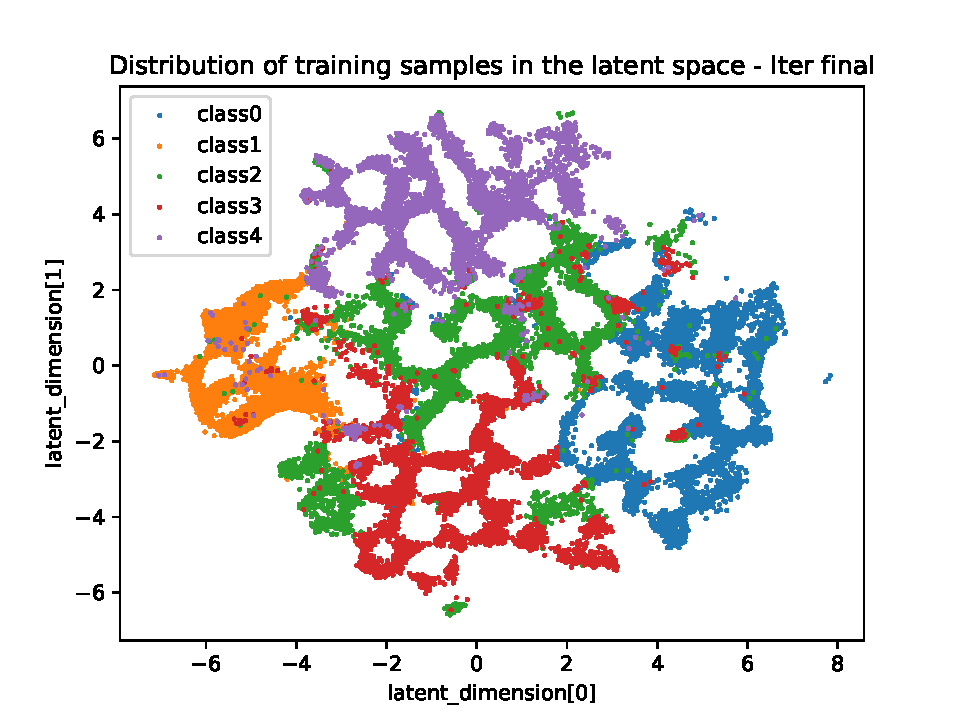
\includegraphics[width=\textwidth]{mnist_5classes_2dim.pdf}
    \end{minipage}
    \begin{minipage}{.49\textwidth}
        \flushright
        \setlength\figureheight{.49\textheight}
        \setlength\figurewidth{.95\textwidth}
        % This file was created by matplotlib2tikz v0.6.11.
\begin{tikzpicture}

\definecolor{color1}{rgb}{0.545098039215686,0.564705882352941,0.619607843137255}
\definecolor{color0}{rgb}{0.898039215686275,0.898039215686275,0.968627450980392}
\definecolor{color2}{rgb}{0.207843137254902,0.447058823529412,0.776470588235294}

\begin{axis}[
ylabel={RMSE},
xmin=36.451, xmax=7203.382,
ymin=0.13145, ymax=0.95315,
width=\figurewidth,
height=\figureheight,
tick align=outside,
tick pos=left,
xmajorgrids,
x grid style={color0},
ymajorgrids,
y grid style={color0},
axis line style={color1},
legend style={draw=white!80.0!black},
legend entries={{MNIST}},
legend cell align={left}
]
\addplot [semithick, color2]
table {%
36.451 0.9158
72.44 0.8192
108.586 0.7462
144.561 0.6814
180.578 0.6316
216.655 0.5894
252.676 0.5481
288.564 0.5167
324.56 0.4885
360.704 0.4683
396.71 0.4426
432.771 0.4251
468.631 0.4084
504.484 0.3919
540.642 0.3766
576.35 0.365
612.317 0.3551
648.373 0.3464
684.351 0.333
720.229 0.3247
756.217 0.3163
792.209 0.3087
828.109 0.3013
864.092 0.2941
900.174 0.2876
936.199 0.2795
972.152 0.2765
1007.977 0.2711
1044.141 0.2661
1079.941 0.2613
1115.905 0.2565
1151.823 0.2525
1187.73 0.2485
1223.802 0.2458
1259.808 0.2415
1295.743 0.2382
1331.59 0.2353
1367.787 0.2313
1403.677 0.2299
1439.688 0.2268
1475.798 0.2244
1511.745 0.2226
1547.798 0.2204
1583.935 0.2173
1619.936 0.2156
1655.934 0.2141
1691.725 0.2122
1727.661 0.2099
1763.852 0.2089
1799.73 0.207
1835.696 0.2059
1871.732 0.2045
1907.641 0.2028
1943.472 0.2019
1979.491 0.2004
2015.184 0.1993
2051.18 0.1986
2087.218 0.1971
2123.237 0.1962
2159.051 0.1956
2194.938 0.1945
2230.822 0.1932
2266.722 0.1926
2302.801 0.1919
2338.751 0.1909
2374.882 0.1902
2410.816 0.1896
2447.074 0.1887
2482.933 0.1884
2518.978 0.1875
2554.935 0.187
2590.892 0.1866
2626.952 0.1863
2662.884 0.1855
2698.794 0.1849
2735.36 0.1776
2771.376 0.1766
2807.2 0.176
2843.315 0.1757
2879.216 0.1754
2915.285 0.1752
2951.146 0.175
2987.208 0.1748
3023.231 0.1746
3059.311 0.1745
3095.184 0.1744
3131.249 0.1742
3167.371 0.1741
3203.392 0.174
3239.484 0.1739
3275.273 0.1738
3311.348 0.1737
3347.328 0.1736
3383.29 0.1735
3419.216 0.1735
3455.202 0.1733
3491.361 0.1733
3527.34 0.1732
3563.345 0.1731
3599.398 0.173
3635.679 0.173
3671.731 0.1729
3707.722 0.1728
3743.692 0.1727
3779.707 0.1727
3815.692 0.1726
3851.555 0.1725
3887.61 0.1725
3923.668 0.1724
3959.738 0.1723
3995.807 0.1723
4031.611 0.1722
4067.608 0.1721
4103.552 0.1721
4139.571 0.172
4175.36 0.172
4211.334 0.1719
4247.368 0.1718
4283.419 0.1718
4319.386 0.1717
4355.327 0.1717
4391.379 0.1716
4427.72 0.1715
4463.72 0.1715
4499.496 0.1714
4535.373 0.1714
4571.453 0.1713
4607.407 0.1713
4643.496 0.1712
4679.241 0.1712
4715.096 0.1712
4751.16 0.1711
4787.158 0.1711
4823.234 0.171
4859.312 0.171
4895.332 0.1709
4931.436 0.1709
4967.378 0.1708
5003.414 0.1707
5039.401 0.1707
5075.873 0.1706
5112.414 0.1705
5148.599 0.1705
5184.582 0.1704
5220.877 0.1704
5256.921 0.1703
5292.75 0.1703
5328.896 0.1703
5364.954 0.1702
5401.143 0.1702
5437.187 0.1702
5473.071 0.1701
5509.127 0.1701
5545.19 0.17
5581.158 0.17
5617.267 0.17
5653.163 0.1699
5689.197 0.1699
5725.389 0.1698
5761.315 0.1698
5797.307 0.1698
5833.548 0.1697
5869.866 0.1697
5905.342 0.1697
5941.405 0.1696
5977.493 0.1696
6013.597 0.1696
6049.582 0.1696
6085.602 0.1695
6121.56 0.1695
6157.577 0.1695
6193.91 0.1694
6230.347 0.1694
6266.426 0.1694
6302.589 0.1693
6338.509 0.1693
6374.421 0.1693
6410.598 0.1693
6446.635 0.1692
6482.777 0.1692
6518.88 0.1692
6554.903 0.1692
6590.847 0.1691
6626.816 0.1691
6663.012 0.1691
6699.022 0.1691
6735.009 0.169
6771.22 0.169
6807.302 0.169
6843.313 0.169
6879.181 0.169
6915.342 0.1689
6951.374 0.1689
6987.394 0.1689
7023.401 0.1689
7059.466 0.1688
7095.553 0.1688
7131.51 0.1688
7167.283 0.1688
7203.382 0.1688
};
\end{axis}

\end{tikzpicture}
\\
        \flushright
        % This file was created by matplotlib2tikz v0.6.11.
\begin{tikzpicture}

\definecolor{color1}{rgb}{0.545098039215686,0.564705882352941,0.619607843137255}
\definecolor{color0}{rgb}{0.898039215686275,0.898039215686275,0.968627450980392}
\definecolor{color2}{rgb}{1,0.647058823529412,0}

\begin{axis}[
ylabel={Neg. loglik.},
xmin=36.451, xmax=7203.382,
ymin=-414.881931, ymax=2498.313651,
width=\figurewidth,
height=\figureheight,
tick align=outside,
tick pos=left,
xmajorgrids,
x grid style={color0},
ymajorgrids,
y grid style={color0},
axis line style={color1},
legend style={draw=white!80.0!black},
legend entries={{MNIST}},
legend cell align={left}
]
\addplot [semithick, color2]
table {%
36.451 2365.89567
72.44 1880.18512
108.586 1549.13335
144.561 1281.30828
180.578 1091.88698
216.655 942.5874
252.676 806.50732
288.564 709.82076
324.56 627.73807
360.704 571.6008
396.71 503.79981
432.771 459.90862
468.631 419.56573
504.484 381.25258
540.642 347.26585
576.35 322.37371
612.317 301.77396
648.373 284.0555
684.351 257.69002
720.229 241.74139
756.217 226.27897
792.209 212.40056
828.109 199.43568
864.092 187.0623
900.174 176.07346
936.199 162.76665
972.152 157.85114
1007.977 149.31733
1044.141 141.61962
1079.941 134.1498
1115.905 126.99837
1151.823 121.16218
1187.73 115.28398
1223.802 111.38158
1259.808 105.36137
1295.743 100.75394
1331.59 96.85886
1367.787 91.43352
1403.677 89.56818
1439.688 85.43711
1475.798 82.29648
1511.745 79.96238
1547.798 77.18816
1583.935 73.19888
1619.936 71.05707
1655.934 69.23152
1691.725 66.92545
1727.661 64.09648
1763.852 62.82099
1799.73 60.56308
1835.696 59.29079
1871.732 57.58808
1907.641 55.56713
1943.472 54.46814
1979.491 52.7669
2015.184 51.48593
2051.18 50.63524
2087.218 48.99993
2123.237 47.95905
2159.051 47.24331
2194.938 46.03876
2230.822 44.52205
2266.722 43.84857
2302.801 43.08497
2338.751 42.01794
2374.882 41.2691
2410.816 40.56116
2447.074 39.60253
2482.933 39.29827
2518.978 38.22697
2554.935 37.72695
2590.892 37.34902
2626.952 36.93567
2662.884 36.12898
2698.794 35.48449
2735.36 -242.61165
2771.376 -247.10751
2807.2 -249.4782
2843.315 -251.04296
2879.216 -252.37654
2915.285 -253.25399
2951.146 -254.26752
2987.208 -255.01126
3023.231 -255.81305
3059.311 -256.36644
3095.184 -256.96792
3131.249 -257.5522
3167.371 -258.0024
3203.392 -258.59452
3239.484 -258.94638
3275.273 -259.42993
3311.348 -259.91921
3347.328 -260.27134
3383.29 -260.60549
3419.216 -260.99034
3455.202 -261.48786
3491.361 -261.84993
3527.34 -262.14832
3563.345 -262.47807
3599.398 -262.87405
3635.679 -263.22787
3671.731 -263.57825
3707.722 -263.79496
3743.692 -264.21214
3779.707 -264.51557
3815.692 -264.89443
3851.555 -265.13449
3887.61 -265.46882
3923.668 -265.74609
3959.738 -266.07145
3995.807 -266.34493
4031.611 -266.69022
4067.608 -266.90746
4103.552 -267.22429
4139.571 -267.5522
4175.36 -267.81808
4211.334 -268.10621
4247.368 -268.37802
4283.419 -268.65749
4319.386 -268.94383
4355.327 -269.2154
4391.379 -269.52334
4427.72 -269.68264
4463.72 -269.88745
4499.496 -270.11269
4535.373 -270.3551
4571.453 -270.60411
4607.407 -270.89682
4643.496 -271.04399
4679.241 -271.21676
4715.096 -271.43313
4751.16 -271.63257
4787.158 -271.87858
4823.234 -272.1199
4859.312 -272.39825
4895.332 -272.58972
4931.436 -272.81499
4967.378 -272.95959
5003.414 -273.26811
5039.401 -273.6122
5075.873 -274.03817
5112.414 -274.31779
5148.599 -274.54465
5184.582 -274.76546
5220.877 -275.02458
5256.921 -275.21931
5292.75 -275.38793
5328.896 -275.55834
5364.954 -275.76582
5401.143 -275.90669
5437.187 -276.02925
5473.071 -276.20526
5509.127 -276.3756
5545.19 -276.58812
5581.158 -276.73742
5617.267 -277.00069
5653.163 -277.14499
5689.197 -277.31586
5725.389 -277.45682
5761.315 -277.61711
5797.307 -277.76919
5833.548 -277.92725
5869.866 -278.15705
5905.342 -278.27376
5941.405 -278.42473
5977.493 -278.55824
6013.597 -278.71366
6049.582 -278.82135
6085.602 -279.00605
6121.56 -279.19025
6157.577 -279.19398
6193.91 -279.35256
6230.347 -279.57717
6266.426 -279.65943
6302.589 -279.86358
6338.509 -279.94947
6374.421 -280.09387
6410.598 -280.19941
6446.635 -280.34766
6482.777 -280.40881
6518.88 -280.54154
6554.903 -280.61047
6590.847 -280.73751
6626.816 -280.84645
6663.012 -280.89839
6699.022 -281.06017
6735.009 -281.21081
6771.22 -281.30197
6807.302 -281.38414
6843.313 -281.46418
6879.181 -281.61276
6915.342 -281.78268
6951.374 -281.85253
6987.394 -281.88172
7023.401 -282.07926
7059.466 -282.0955
7095.553 -282.19136
7131.51 -282.30292
7167.283 -282.39453
7203.382 -282.46395
};
\end{axis}

\end{tikzpicture}

    \end{minipage}

\end{frame}

\subsection{Experiments on Clustering}

\begin{frame}{Experiments on Clustering - Blobs}
    \begin{minipage}{.49\textwidth}
        \centering
        \setlength\figureheight{.65\textheight}
        \setlength\figurewidth{1.2\textwidth}
        % This file was created by matplotlib2tikz v0.6.11.
\begin{tikzpicture}

\definecolor{color1}{rgb}{1,0.498039215686275,0.0549019607843137}
\definecolor{color0}{rgb}{0.12156862745098,0.466666666666667,0.705882352941177}
\definecolor{color2}{rgb}{0.172549019607843,0.627450980392157,0.172549019607843}
\pgfplotsset{ticks=none}
\begin{axis}[
xmin=-11.254671248187, xmax=-0.408519973755034,
ymin=-9.66339497832892, ymax=6.11370945265441,
width=\figurewidth,
height=\figureheight,
tick pos=left
]
\addplot [only marks, mark size=0.5pt, draw=color0, fill=color0, colormap/viridis]
table{%
x                      y
-2.009263110615139e+00 +4.426931823544566e+00
-9.018456278555119e-01 +4.612636025101525e+00
-1.399537617659996e+00 +4.176879859268155e+00
-1.827225477520777e+00 +4.500880815423391e+00
-1.513398253329163e+00 +4.487558429705267e+00
-1.303656298611273e+00 +4.632489662344043e+00
-1.369199910529921e+00 +4.399607522276167e+00
-1.449344516413244e+00 +4.380768064449777e+00
-1.359830435973143e+00 +4.452778973214148e+00
-1.742380698431677e+00 +4.503124655126435e+00
-1.384810822761725e+00 +4.181081246224162e+00
-1.378706865443036e+00 +4.482806628904164e+00
-1.553686317432491e+00 +4.425824885930301e+00
-1.623997062816940e+00 +4.534866238840299e+00
-1.719045389886565e+00 +4.695311840365218e+00
-1.590435079742974e+00 +4.223171967869333e+00
-1.755767968156717e+00 +4.771016928495541e+00
-1.798933586395030e+00 +4.641282054892283e+00
-1.740164206951896e+00 +4.310476280176058e+00
-1.459094647980683e+00 +4.418131693449198e+00
-1.745523324841288e+00 +4.417389083051723e+00
-1.827371438657724e+00 +4.403323719113436e+00
-1.546779171264870e+00 +4.232759643546852e+00
-1.456821987747630e+00 +4.667600392519976e+00
-1.413321988018717e+00 +4.674302975804634e+00
-1.765683103591251e+00 +4.223607123410578e+00
-1.533763702589688e+00 +4.729796339476227e+00
-1.996501141261935e+00 +4.774174833016004e+00
-1.878880285678067e+00 +4.189543063124930e+00
-1.457348815882099e+00 +4.853928539644730e+00
-1.836020032799091e+00 +4.704661385781835e+00
-1.597360115601577e+00 +4.332329580750446e+00
-2.072240222404544e+00 +4.183850972802399e+00
-1.612919558201448e+00 +4.509002780645226e+00
-1.567751952477553e+00 +4.714714666937221e+00
-1.706204654326386e+00 +4.392283748621700e+00
-1.558686995500820e+00 +4.554884499652428e+00
-1.584517325959563e+00 +4.318427407219782e+00
-1.252647217661293e+00 +4.490992792986781e+00
-1.791602844014383e+00 +4.138247713304119e+00
-1.938887493107339e+00 +4.465093793297434e+00
-1.716751363166060e+00 +4.809830212483940e+00
-1.581991834002578e+00 +3.882927914787459e+00
-1.669233783265032e+00 +4.002546780167338e+00
-2.262935656241966e+00 +3.962098274891665e+00
-1.455548984867504e+00 +4.253388125560956e+00
-1.566445693070659e+00 +4.369367418078313e+00
-1.729993973214923e+00 +4.920578749642734e+00
-1.601436266153835e+00 +4.577127720559282e+00
-1.504109029872126e+00 +4.256538736075449e+00
-1.332133429527856e+00 +4.117744210110820e+00
-1.376652559085663e+00 +4.786444072948711e+00
-2.068922304200605e+00 +5.396140544852653e+00
-1.695358842200329e+00 +4.664735813580600e+00
-1.369475263450077e+00 +4.498863047937093e+00
-2.134262920778343e+00 +4.127212195733383e+00
-1.654094196791881e+00 +4.289321414773688e+00
-1.550018319125710e+00 +4.687071949257435e+00
-1.701609615884699e+00 +4.362944782766164e+00
-1.312365056855952e+00 +4.241153808054907e+00
-1.392317000398204e+00 +4.416582726598872e+00
-1.759779453895751e+00 +4.612491273455763e+00
-2.044258217384680e+00 +4.294516072664132e+00
-1.867102879777298e+00 +4.186345468882119e+00
-1.442338366697053e+00 +4.594092778809413e+00
-1.936488031519658e+00 +4.402060289365626e+00
-1.796003447944162e+00 +4.356780403120937e+00
-1.893038569855145e+00 +4.273234787322262e+00
-1.669354470000894e+00 +4.349301326038108e+00
-1.529415821680177e+00 +4.120404521437376e+00
-1.527193574860342e+00 +4.440915171342508e+00
-1.546738901938477e+00 +3.985474872376102e+00
-1.927800975626431e+00 +4.530279521643241e+00
-1.729334336334342e+00 +4.812202140331662e+00
-1.341120923408825e+00 +4.898265306156845e+00
-1.407028111614838e+00 +4.636494352155102e+00
-1.938677410419706e+00 +4.426721644086481e+00
-1.434162225800321e+00 +4.532113453568629e+00
-1.934714700251750e+00 +4.692670796303065e+00
-1.527339969552226e+00 +3.847218241065044e+00
-1.646857967254512e+00 +4.247240957200823e+00
-1.872423820081226e+00 +4.656710224763237e+00
-1.687171662552849e+00 +4.252149352915072e+00
-1.588163074634955e+00 +4.627775159910843e+00
-1.575254671371405e+00 +4.658506227112102e+00
-1.536475766964357e+00 +4.236320333590940e+00
-1.206926177417155e+00 +4.080058138203727e+00
-1.773589294735691e+00 +4.161517305927712e+00
-2.020588357305917e+00 +4.280373403106549e+00
-1.598892545678071e+00 +4.456947413561663e+00
-1.800136263703292e+00 +4.895209387595420e+00
-1.660032776658021e+00 +4.057334762694303e+00
-2.050994443612496e+00 +4.659945485586088e+00
-1.307674905888212e+00 +4.438765263770843e+00
-1.688556202316619e+00 +4.362625126677723e+00
-1.446383890517198e+00 +4.415329893106851e+00
-1.689676048895646e+00 +4.098209684981555e+00
-1.955139437575928e+00 +4.240051239293380e+00
-1.614300219859052e+00 +4.683283731580427e+00
-1.650824008607584e+00 +4.769969264245366e+00
-1.486416319063681e+00 +4.286821779739246e+00
-1.448019744052261e+00 +4.191610883635165e+00
-1.494304834048846e+00 +4.854529421087054e+00
-1.846349479386229e+00 +4.829603519100099e+00
-2.024910807129046e+00 +4.277402891681656e+00
-1.832475093879847e+00 +4.307301487129167e+00
-1.814560116935552e+00 +4.580997877361217e+00
-1.865176703174583e+00 +4.586917691871335e+00
-1.686174936337405e+00 +3.708740767169700e+00
-1.703967954944407e+00 +4.028875775071270e+00
-1.726531925855024e+00 +4.539078735527708e+00
-1.731809241700974e+00 +4.308535808891150e+00
-1.552178370943028e+00 +4.254740269293150e+00
-1.764294380368050e+00 +4.286693640061310e+00
-1.555234404704804e+00 +4.602682531597059e+00
-1.624149771532068e+00 +3.777413903601724e+00
-1.312981339886940e+00 +4.543522265015210e+00
-1.915031392108847e+00 +4.605121928743432e+00
-1.446239600459614e+00 +4.303232541415404e+00
-1.296702590800786e+00 +4.251980656922766e+00
-1.380964161753572e+00 +4.259858884137763e+00
-2.089408524603400e+00 +4.420770117863684e+00
-1.146766545234158e+00 +4.552905368886258e+00
-1.834659532178833e+00 +4.355641256602022e+00
-1.500414053594862e+00 +4.758803216184163e+00
-1.143114075893811e+00 +4.038700637385006e+00
-1.708324241167495e+00 +4.607838224901207e+00
-1.294336810832750e+00 +4.554608069199166e+00
-1.737089099328035e+00 +3.797780427816377e+00
-2.216338063911023e+00 +3.981656467662587e+00
-1.417925093391255e+00 +4.584752131418979e+00
-1.461358189468683e+00 +4.250607186423213e+00
-1.269858520793555e+00 +4.433840542949518e+00
-1.602036222107424e+00 +4.596992663921168e+00
-1.254331834543083e+00 +4.204943664497605e+00
-1.859446778621459e+00 +4.333591219967953e+00
-1.644372356998643e+00 +4.459271057595091e+00
-1.704789981468057e+00 +4.255509711894847e+00
-1.244609361671052e+00 +4.592000908987496e+00
-1.503719361804011e+00 +4.297750698104355e+00
-1.629520167828112e+00 +4.560790646270016e+00
-1.888507868215689e+00 +4.304676858088170e+00
-2.286170069117535e+00 +3.877948888363955e+00
-1.508980085874612e+00 +4.511560419754926e+00
-2.098541316006732e+00 +4.585187268214615e+00
-1.964496005193278e+00 +5.018832031108511e+00
-1.463253176039848e+00 +4.240272927101358e+00
-1.398311303530045e+00 +4.558618543464374e+00
-1.566642333145553e+00 +4.869742240110506e+00
-1.379205478889604e+00 +4.508715003327368e+00
-1.465205104636304e+00 +4.376797075817390e+00
-1.488559573903031e+00 +4.318137373126408e+00
-1.406758140004792e+00 +4.037349203713116e+00
-1.443207998617350e+00 +3.831105194623091e+00
-1.939338755588452e+00 +4.895509594769072e+00
-1.372834811848649e+00 +4.394064224053492e+00
-1.504289230738767e+00 +4.645520294874336e+00
-1.753261077774183e+00 +4.218997464524245e+00
-1.693554237473667e+00 +4.207172422469879e+00
-1.236107627626499e+00 +4.455707313655735e+00
-1.771342047145019e+00 +4.712616795044537e+00
-1.635703634150705e+00 +4.636852386008039e+00
-1.505063522468436e+00 +4.360445787429725e+00
-1.438103456207043e+00 +4.453955281188936e+00
-1.494797456923467e+00 +3.999630283689097e+00
-1.333008389664657e+00 +4.255339126552068e+00
-1.821289078012247e+00 +4.631861591755340e+00
-1.949602432194089e+00 +4.744016573513593e+00
-2.145821645601529e+00 +4.177633776785235e+00
-2.195176588217862e+00 +4.198947652837485e+00
-1.542899089141309e+00 +4.664911585828037e+00
-1.626047856809864e+00 +4.707003584393088e+00
-1.770117225826813e+00 +4.487371707243519e+00
-1.567976902313505e+00 +4.145342523366214e+00
-1.709309451899451e+00 +4.873107712631192e+00
-1.665714144917464e+00 +4.212699464050871e+00
-1.937918931691767e+00 +4.389637362606448e+00
-1.530706455502709e+00 +4.127772105751677e+00
-1.698808324071849e+00 +4.072689188089363e+00
-1.730275793857231e+00 +4.339908147763482e+00
-1.464553122113862e+00 +4.249129467829716e+00
-1.655428014122116e+00 +4.450786798912151e+00
-1.763271631270579e+00 +4.519476378173468e+00
-1.518869631793763e+00 +4.466674141902595e+00
-1.561282594735024e+00 +3.950509905686863e+00
-1.449814052479893e+00 +4.639265389169051e+00
-1.474420793174451e+00 +4.168064718391178e+00
-1.834896012512814e+00 +4.272184112874327e+00
-2.106538128748448e+00 +4.496951697803054e+00
-1.704462979611359e+00 +4.531921146179453e+00
-1.223356964894400e+00 +4.216188143619386e+00
-1.718669143901766e+00 +4.588443243843074e+00
-1.489542445978993e+00 +4.326539469118494e+00
-1.473720770070054e+00 +4.029096697787151e+00
-1.690282462328182e+00 +4.172547510278394e+00
-1.861771705066552e+00 +4.545849732057670e+00
-1.687057778489421e+00 +4.408627105202168e+00
-1.705409955278526e+00 +4.681739919510282e+00
-1.771744414116425e+00 +4.238377859146512e+00
-1.877061961746233e+00 +4.498787486229880e+00
-1.685896084075405e+00 +4.564038786514390e+00
-1.668401887168197e+00 +4.934141132243339e+00
-2.002839236010209e+00 +4.485279716853735e+00
-1.933848496012360e+00 +4.616148555650256e+00
-1.145903880318991e+00 +4.419842253042749e+00
-2.054348977297136e+00 +4.199332874129060e+00
-1.779349180645039e+00 +4.494031658550231e+00
-1.441817455315459e+00 +4.279375585274312e+00
-1.854024612605373e+00 +4.685450145824204e+00
-1.656221736861725e+00 +4.232816470021355e+00
-1.497398994925853e+00 +4.433325692299059e+00
-1.255322506234195e+00 +4.532175089343138e+00
-1.629104588200660e+00 +4.688860845821141e+00
-2.124055372060208e+00 +4.715530876456366e+00
-1.706202348925357e+00 +4.381053400710875e+00
-1.222951133641526e+00 +4.212722297074802e+00
-1.531825462325497e+00 +4.834155328510946e+00
-1.589393636667860e+00 +4.388211692906342e+00
-1.736110909105613e+00 +4.613483529494973e+00
-1.531327450844017e+00 +4.331966660067483e+00
-1.800507089594095e+00 +4.428911470673809e+00
-1.125102889088649e+00 +4.210106369613102e+00
-1.992547822577832e+00 +3.966317728743466e+00
-1.326695627801622e+00 +4.334662902974157e+00
-1.486218349533423e+00 +4.216973036704103e+00
-1.649006469269621e+00 +4.552193672272117e+00
-1.376117545364660e+00 +4.131517052014654e+00
-1.715141941601109e+00 +4.356300351610662e+00
-1.494139636832024e+00 +4.653077913896178e+00
-1.788833520428577e+00 +4.157233161930596e+00
-1.792618411173064e+00 +4.686023218022585e+00
-1.546655918309709e+00 +4.682533450418965e+00
-2.147586227759827e+00 +4.055907582479877e+00
-1.707518794038923e+00 +4.184582627821952e+00
-1.929737579059896e+00 +4.587858369963546e+00
-1.504925123251946e+00 +4.295696886168002e+00
-2.168860212368718e+00 +3.920842573474048e+00
-1.774545613658691e+00 +4.567578285350742e+00
-1.537430369314145e+00 +4.387596940587898e+00
-1.986193424159524e+00 +4.425584988883060e+00
-1.460043957123784e+00 +4.381006859027262e+00
-1.571923411282493e+00 +4.078419016033804e+00
-1.676892080121140e+00 +4.379391852049777e+00
-1.786802975404235e+00 +4.364868380121671e+00
-1.726114532449425e+00 +4.414643505516501e+00
-1.784113296856289e+00 +4.328743624267449e+00
-1.434345918632417e+00 +4.235557904049578e+00
-1.446239359492586e+00 +4.371561936232894e+00
-1.588372878236255e+00 +4.472106730208979e+00
-1.265692928805424e+00 +4.708141843352053e+00
-1.959376914032316e+00 +4.622326198229167e+00
-1.113166054315229e+00 +4.057365784971127e+00
-1.633004224939715e+00 +4.025069789785822e+00
-1.765274146296213e+00 +4.428105970474233e+00
-1.611831034781653e+00 +4.931553652962872e+00
-1.360102195518207e+00 +4.832638411686263e+00
-1.776098620155002e+00 +4.752737704755321e+00
-1.627465658409533e+00 +4.846593664736992e+00
-1.580651169138118e+00 +3.900939564887161e+00
-1.809849106110865e+00 +4.545508246362508e+00
-1.399853755483666e+00 +4.953234780586726e+00
-1.111884973706086e+00 +3.932399638120388e+00
-1.571780681820778e+00 +4.389297253073502e+00
-1.933287867383780e+00 +4.448835477107829e+00
-1.547021027756725e+00 +4.847823643972929e+00
-1.183395228863274e+00 +4.684254043483287e+00
-2.357831155985155e+00 +4.890872072247181e+00
-1.728521421588805e+00 +4.713728765255836e+00
-1.840959185732126e+00 +4.189547699437264e+00
-1.298840673824442e+00 +4.271569478292538e+00
-1.762469696745640e+00 +4.726121889553592e+00
-1.460803382342308e+00 +4.312880289132356e+00
-1.588890977886414e+00 +4.199965510881332e+00
-1.977699594760018e+00 +4.484876798959020e+00
-1.640104623970343e+00 +4.561084934342793e+00
-1.200880499286098e+00 +4.547585582716740e+00
-1.579800131934245e+00 +4.344147274973809e+00
-2.016198761078653e+00 +4.848479855920918e+00
-1.908814854830940e+00 +4.379791372148356e+00
-1.648642657653922e+00 +4.349911308214760e+00
-2.019778912021479e+00 +4.714553136550270e+00
-1.609984975916827e+00 +4.436242030295026e+00
-1.619550638586562e+00 +4.625532099122218e+00
-1.855037826620220e+00 +4.297112623136016e+00
-1.722478457856376e+00 +4.502168662274252e+00
-1.490960879743302e+00 +4.225891892489623e+00
-1.617092592111627e+00 +4.115487876052861e+00
-1.897575431125084e+00 +4.276953480743472e+00
-1.968773250083869e+00 +4.625449600755486e+00
-1.945189455454055e+00 +4.319154188239942e+00
-1.741184780468066e+00 +4.070820921498803e+00
-1.535757074954029e+00 +4.362814078907537e+00
-1.544268880954265e+00 +4.112494200982833e+00
-1.831353080978419e+00 +4.195188458468482e+00
-1.530791502538678e+00 +3.710856251929931e+00
-1.898416221541942e+00 +4.552967476618815e+00
-1.549218795056374e+00 +4.381451060522287e+00
-1.367791114448528e+00 +4.396572693820541e+00
-1.967074439865260e+00 +4.544124242837215e+00
-1.620493943380999e+00 +4.358934612571947e+00
-2.078108857853253e+00 +4.612747324952908e+00
-1.450558726089952e+00 +4.792329646544283e+00
-1.711783464292214e+00 +4.553145666638711e+00
-1.745535083251118e+00 +4.156447571375033e+00
-1.874888996142530e+00 +4.575167750265154e+00
-1.027478479246920e+00 +4.344331174414297e+00
-1.919355486457245e+00 +4.589745676772931e+00
-1.219497599336246e+00 +4.391326745899459e+00
-1.495914867801844e+00 +4.393692756941245e+00
-2.127850150357345e+00 +4.636643648356901e+00
-1.741822793283790e+00 +4.743266235010786e+00
-2.145390757365608e+00 +4.494613459935495e+00
-1.848159391197683e+00 +4.719706907651483e+00
-1.412976108993209e+00 +4.459873344177022e+00
-1.680686912799677e+00 +4.332149398149785e+00
-1.815895406315017e+00 +4.258029102029534e+00
-1.294032921687276e+00 +3.891454691468748e+00
-1.702666957836128e+00 +4.187025264362819e+00
-1.353270943630212e+00 +4.143103350418083e+00
-1.753381143471048e+00 +4.246807266979606e+00
-1.851387362531453e+00 +4.575132545582163e+00
-1.807895844509124e+00 +4.534066768029476e+00
-1.655268724354998e+00 +4.299204299284388e+00
-1.357445823810529e+00 +4.685415319539283e+00
-1.921826842240673e+00 +4.485654592632325e+00
-1.778403124733015e+00 +4.525892414297551e+00
-1.469858490924037e+00 +4.627717072459382e+00
-1.655207553873518e+00 +4.125985186656440e+00
-1.715163413080997e+00 +4.774029954799596e+00
-1.745806708487264e+00 +4.348779933059294e+00
-1.723104872850362e+00 +4.756450854463408e+00
-1.808476876176092e+00 +4.329209539182696e+00
-1.724305619298653e+00 +4.453813168232826e+00
-1.693671091922528e+00 +4.376726321899459e+00
};
\addplot [only marks, mark size=0.5pt, draw=color1, fill=color1, colormap/viridis]
table{%
x                      y
-9.650719051265860e+00 -3.896798608152416e+00
-9.833078285763152e+00 -3.703623135114885e+00
-1.022607335606680e+01 -4.109324835530370e+00
-9.623611175813048e+00 -3.535666241935473e+00
-9.621582036986933e+00 -4.097955290496116e+00
-1.006930873250190e+01 -4.171070459776195e+00
-1.038381144899978e+01 -4.339988807355369e+00
-9.931301903024529e+00 -4.018465062079549e+00
-9.971699156225830e+00 -3.821347691845245e+00
-1.004744686622407e+01 -3.877858536011668e+00
-1.013999966703109e+01 -4.218797737690917e+00
-9.855431354696906e+00 -3.904019549426257e+00
-1.008836552554742e+01 -4.324637660194568e+00
-1.007635346913242e+01 -4.289601052430299e+00
-9.925558324733901e+00 -3.938771701677183e+00
-9.906875524009536e+00 -4.198278595224449e+00
-1.013247064865811e+01 -3.792323550377471e+00
-9.873395228991606e+00 -3.894015372528306e+00
-1.027223329000836e+01 -3.763689281607843e+00
-9.932243633918016e+00 -4.100105798651906e+00
-1.004838598057997e+01 -3.916935593041583e+00
-1.023802840341073e+01 -4.317929662461493e+00
-1.002825100743102e+01 -4.123561440867534e+00
-1.009259188253657e+01 -4.207049470077872e+00
-1.008700938505386e+01 -4.083692643715214e+00
-1.033488661535241e+01 -3.627714663241659e+00
-1.025366233273465e+01 -3.811407362449291e+00
-1.051691300913399e+01 -3.716473255526786e+00
-1.030368241629691e+01 -3.813782492721295e+00
-9.723040378391321e+00 -3.665045392019524e+00
-1.000001288971395e+01 -3.786695876011677e+00
-1.004534957806846e+01 -3.895013765798174e+00
-9.613578421647826e+00 -3.953442299552794e+00
-9.979649528864130e+00 -3.700901713626315e+00
-9.877500975336810e+00 -3.926018956386846e+00
-9.727948239915419e+00 -4.125056453807802e+00
-9.709562719900450e+00 -4.009407490394080e+00
-9.667039007375941e+00 -3.904804793289760e+00
-1.022238330198276e+01 -3.873434311877056e+00
-9.845516588926074e+00 -4.423701264154720e+00
-1.019541249209689e+01 -3.647417994373177e+00
-9.847909194788286e+00 -4.320907819618533e+00
-9.167442814610510e+00 -4.103404879957534e+00
-9.925692961901813e+00 -3.578821501468946e+00
-9.439032069246631e+00 -3.941636996148629e+00
-9.607107621279861e+00 -4.171048935515220e+00
-9.898062906612742e+00 -4.001349471520966e+00
-1.010726257048777e+01 -3.906964642121566e+00
-1.062644365975455e+01 -3.749692293617132e+00
-9.715774667415545e+00 -3.940775237606442e+00
-1.029298829684606e+01 -4.068331073471850e+00
-9.862051180011523e+00 -4.442890818762957e+00
-1.031492724344655e+01 -3.513658709842246e+00
-9.775452664477577e+00 -3.497143850715708e+00
-9.633580657034907e+00 -3.874189238437215e+00
-9.899105496150073e+00 -3.771967907799815e+00
-1.043506385908541e+01 -3.621867876491084e+00
-9.830742613312017e+00 -3.960922742222908e+00
-1.021208670983804e+01 -4.186894008150192e+00
-9.692743908895446e+00 -4.236796556211599e+00
-9.546815258281477e+00 -4.066479790684211e+00
-1.006142574046407e+01 -3.988576235460744e+00
-1.009699392436714e+01 -3.731826067311457e+00
-9.989558632863933e+00 -4.272757631133513e+00
-9.751709444418042e+00 -4.093268902842844e+00
-1.031532769774947e+01 -3.882599663910454e+00
-1.007295654214194e+01 -3.751484568111887e+00
-9.756706845598746e+00 -3.843109547193094e+00
-9.988663137962993e+00 -3.445849175503089e+00
-1.024215575403634e+01 -3.910359264321307e+00
-9.612910751239335e+00 -4.240524604772441e+00
-1.006480532968325e+01 -3.986267453934959e+00
-9.918208929548308e+00 -4.175916435390267e+00
-9.888962922587391e+00 -3.725742646612434e+00
-9.606040953379065e+00 -4.012785571899546e+00
-1.004769735195842e+01 -3.951501301436659e+00
-9.998438866221987e+00 -3.968506122933015e+00
-9.809878194862980e+00 -3.918249688251367e+00
-1.000566679682780e+01 -3.925226611759656e+00
-9.763925558755332e+00 -3.500216593583819e+00
-1.020159934145429e+01 -4.135830200435114e+00
-1.016318546238802e+01 -3.888590571915204e+00
-9.882767078600555e+00 -4.004931275374425e+00
-9.962685033326913e+00 -4.308135741649326e+00
-1.032626276178481e+01 -4.013799013693923e+00
-1.023946559640515e+01 -3.648919483394367e+00
-9.866524880578895e+00 -4.072629598980537e+00
-1.012830161993702e+01 -4.045662522820447e+00
-1.051931014501723e+01 -3.862898137220443e+00
-9.846953526121426e+00 -3.874740563925087e+00
-9.912840552260855e+00 -3.880115765943062e+00
-1.076115359875968e+01 -3.833385454574750e+00
-9.778662537990511e+00 -3.922534681470006e+00
-9.703449439708940e+00 -4.113625501162677e+00
-9.886438326066958e+00 -3.928820485807707e+00
-9.985231881636137e+00 -3.898479173919346e+00
-1.031756904273148e+01 -4.288400841339080e+00
-9.969878187057359e+00 -3.958229186943273e+00
-1.019158011232908e+01 -3.478970845578367e+00
-9.957571255717474e+00 -3.983386041270392e+00
-1.000064605724724e+01 -4.130973716029944e+00
-9.669488650770669e+00 -3.947509290470790e+00
-9.885617340957680e+00 -3.672017672697141e+00
-1.012370599093868e+01 -3.948859574450498e+00
-1.024325274316027e+01 -4.065175587801549e+00
-9.827467771824589e+00 -3.512696322009043e+00
-1.015631368122831e+01 -4.084624395847939e+00
-9.652742528385364e+00 -3.992559199991897e+00
-1.005120944904348e+01 -3.666866708829624e+00
-1.017537644632330e+01 -3.670566397256964e+00
-1.005524101951592e+01 -4.076102155537982e+00
-1.027029708676680e+01 -3.528301510701823e+00
-9.864921555289046e+00 -3.952348336869361e+00
-9.920258314001229e+00 -3.690518355401017e+00
-1.010938730452238e+01 -3.902254198632914e+00
-9.928796484865583e+00 -4.394160997611013e+00
-1.004432282147407e+01 -4.042158925737445e+00
-1.015302544626066e+01 -3.690694885146387e+00
-9.756157288008517e+00 -3.771869334232999e+00
-1.002082058328850e+01 -4.012817363727413e+00
-1.050976261833829e+01 -3.832377635027874e+00
-1.008751852758079e+01 -3.827003071674975e+00
-9.891961701257282e+00 -3.986910688520784e+00
-9.852629975502294e+00 -4.196665443675514e+00
-1.049466988650176e+01 -3.738026418515342e+00
-1.053382351533521e+01 -4.045739153697563e+00
-9.831692616771258e+00 -4.281179642865578e+00
-9.869109613511521e+00 -3.957661263678134e+00
-1.002793483127468e+01 -4.018488695018792e+00
-1.020770973230616e+01 -4.527900017497668e+00
-9.964650558923156e+00 -4.094157698392569e+00
-1.005137596420961e+01 -3.698036515838479e+00
-1.032864885646024e+01 -3.899265307958086e+00
-1.027566702634698e+01 -4.249986472599457e+00
-9.945438334509221e+00 -3.564594548779932e+00
-9.844654372871089e+00 -3.767127413253041e+00
-9.914433866035226e+00 -4.461483494568601e+00
-1.003255045501583e+01 -4.135482919719380e+00
-9.917969547222986e+00 -3.887131640916762e+00
-9.720558314155683e+00 -4.129078648090747e+00
-1.030964603387956e+01 -3.587781551669336e+00
-9.707391080317649e+00 -3.685857162625672e+00
-1.017052974284364e+01 -3.667707567361899e+00
-1.067230293906961e+01 -4.256683078820381e+00
-9.927923640244435e+00 -3.543210135224387e+00
-9.909061990624894e+00 -4.006441868735860e+00
-1.025909606549732e+01 -3.864527420611647e+00
-1.056703700281819e+01 -3.970754682226987e+00
-1.036372589704825e+01 -3.991971345815837e+00
-9.865724865069966e+00 -4.343628520027877e+00
-9.784765094274272e+00 -3.544697922020851e+00
-9.919652831399851e+00 -4.001678957481706e+00
-1.020474940095017e+01 -3.981030650873479e+00
-9.972614573053214e+00 -3.873017088997558e+00
-9.652772955751548e+00 -3.802735822053302e+00
-9.874127090907507e+00 -4.326896988681876e+00
-1.004057280052248e+01 -3.906614285920206e+00
-9.925015517035925e+00 -4.062862174235111e+00
-1.004347800039359e+01 -4.008605772810289e+00
-1.026468164777474e+01 -3.972518388039638e+00
-1.001255447929023e+01 -3.591101196323646e+00
-9.674964160745979e+00 -3.933388644549133e+00
-1.025703479599185e+01 -4.184483850257217e+00
-9.857302979522251e+00 -3.574660951742642e+00
-1.009638492390199e+01 -4.246301892168486e+00
-9.899265570840772e+00 -4.010383720038319e+00
-9.951804110088570e+00 -3.974955265823656e+00
-1.000671004908490e+01 -3.694088801919728e+00
-1.021775976978850e+01 -3.958098677750034e+00
-1.007586325706937e+01 -3.928047775738625e+00
-9.956546237190800e+00 -3.758805002588313e+00
-1.000678282579153e+01 -4.161447384285377e+00
-9.947772614854944e+00 -3.720168193941181e+00
-1.008709105715785e+01 -3.822684753838674e+00
-1.018662819492859e+01 -3.490489073719827e+00
-9.759088587016180e+00 -3.929411854585671e+00
-9.945624273289539e+00 -4.135436068725047e+00
-9.888715954578998e+00 -4.125220395628248e+00
-9.730466010748373e+00 -4.005786781218843e+00
-9.973683968068221e+00 -3.915335462129848e+00
-1.013024245370312e+01 -4.055158553366187e+00
-1.020672487366620e+01 -3.926449812821076e+00
-9.722153320506767e+00 -4.260742110749812e+00
-9.960370014124379e+00 -3.807826700492369e+00
-9.840918244805220e+00 -3.912646484786507e+00
-9.851057874002890e+00 -3.659553875473866e+00
-9.827887217415686e+00 -3.596461809531368e+00
-1.044464693075756e+01 -3.999801261558287e+00
-9.400176013069723e+00 -3.891992835065925e+00
-9.900778837967364e+00 -4.042048237865873e+00
-9.748786518300475e+00 -4.110464185551902e+00
-1.012049378810081e+01 -3.919755268353266e+00
-9.854471822163912e+00 -3.838861778285769e+00
-1.057472213206018e+01 -3.871581445470863e+00
-1.019925705664147e+01 -3.941083124269929e+00
-1.005440255169550e+01 -4.344475510816004e+00
-9.727439255397828e+00 -3.522250617375233e+00
-9.783209640630330e+00 -4.293047757638687e+00
-9.844030934696239e+00 -4.040594595092093e+00
-9.951159579035700e+00 -3.738777047142653e+00
-1.037548165563065e+01 -4.171204063761944e+00
-9.937586115616261e+00 -4.203205172702750e+00
-9.895146067303891e+00 -3.738380804413977e+00
-1.018966344015924e+01 -4.044483059789864e+00
-9.875072242700691e+00 -4.302169303629537e+00
-9.901311930567021e+00 -3.773775863424619e+00
-1.000216689091659e+01 -4.103383247172108e+00
-1.022848199292418e+01 -3.985897349413623e+00
-9.918248033877537e+00 -4.060015368372818e+00
-9.743074384961131e+00 -3.645708997374523e+00
-9.793812413725382e+00 -4.023850022965945e+00
-1.008656587627614e+01 -3.928612985855080e+00
-1.000917917517054e+01 -4.008031912105132e+00
-9.837980173798149e+00 -4.069763480471662e+00
-1.025541201059280e+01 -4.021333247284343e+00
-9.870716419499256e+00 -4.034356629618206e+00
-1.015189910991839e+01 -3.956674602690079e+00
-1.015933526034910e+01 -4.315596434493716e+00
-1.003141078597703e+01 -3.691043974675063e+00
-9.608040440022506e+00 -3.360916000096979e+00
-9.928686815172282e+00 -4.015102670084638e+00
-9.992419546506063e+00 -3.846183862454733e+00
-9.861029937173996e+00 -4.072693962921370e+00
-1.000207624161215e+01 -3.770497918081938e+00
-9.649192243027993e+00 -4.100543449155335e+00
-1.014673408730002e+01 -3.737942772027904e+00
-9.954198887112669e+00 -3.908862157872802e+00
-1.014582782494142e+01 -4.529575531805739e+00
-9.790238909295324e+00 -3.746400690290147e+00
-9.961021187806379e+00 -3.810397327646957e+00
-9.898242397432639e+00 -4.202351269635304e+00
-9.591846977829830e+00 -3.664237645764793e+00
-1.038588719944731e+01 -3.808732442299144e+00
-9.828260610873148e+00 -4.229991814211176e+00
-1.020521525004502e+01 -4.208228509714633e+00
-1.004760268315215e+01 -4.116999339494449e+00
-9.892813694265712e+00 -3.976118231095000e+00
-9.920383053101936e+00 -3.224021356644927e+00
-1.029667788123422e+01 -3.326853476033536e+00
-9.835731300574873e+00 -4.291260893692623e+00
-1.047152924052222e+01 -3.930916268002042e+00
-9.703901255476088e+00 -3.673373796474170e+00
-1.007693780278519e+01 -3.793102080767328e+00
-9.440143966702681e+00 -4.090538754651301e+00
-9.872355106179770e+00 -4.073002065828501e+00
-9.708897064798563e+00 -3.866834110792036e+00
-1.003108467099462e+01 -3.456707269627604e+00
-9.589789625245402e+00 -3.738125737108597e+00
-1.003602154409487e+01 -4.561475675524983e+00
-9.891232459527398e+00 -3.941078448077797e+00
-9.746689227502729e+00 -3.735097088034322e+00
-9.890981421446680e+00 -4.042995746779531e+00
-1.008483028868293e+01 -3.818922275502983e+00
-1.009249240635331e+01 -3.503868705766177e+00
-1.054296949542359e+01 -3.802782265478570e+00
-9.516758647160371e+00 -4.104843877497854e+00
-9.885158068143641e+00 -3.796489276674927e+00
-9.915340011962732e+00 -4.026493281203182e+00
-1.011264192391262e+01 -3.526977667924344e+00
-1.003533858506571e+01 -3.724473730347562e+00
-9.766337199977505e+00 -4.067595511761589e+00
-9.674915277940382e+00 -3.982459584431121e+00
-9.960208433971150e+00 -3.837464966930288e+00
-1.006301298351723e+01 -3.737532697628851e+00
-9.917396025032144e+00 -4.134652278799546e+00
-9.850202637612893e+00 -4.123194493112513e+00
-9.745720884252957e+00 -3.855264819582128e+00
-9.818158408012637e+00 -4.139891975027542e+00
-1.010538266042159e+01 -4.102840682988264e+00
-9.871449065580077e+00 -4.020099592198683e+00
-9.970704799325015e+00 -3.945994142620513e+00
-9.589728541489345e+00 -4.053795755821176e+00
-9.356349308473906e+00 -4.069377273775256e+00
-1.032152697497337e+01 -3.934768408942547e+00
-9.529636688084270e+00 -3.761394015115489e+00
-1.022087417203132e+01 -3.993648127248514e+00
-9.973963476135811e+00 -3.933160800207450e+00
-1.035001482277115e+01 -3.670667208730922e+00
-1.017312463669409e+01 -4.055190968656801e+00
-1.005452563099319e+01 -4.135217574793155e+00
-1.022943048845526e+01 -3.998953648953979e+00
-1.035379592244835e+01 -3.629802969048411e+00
-9.953920571348585e+00 -3.966719470546994e+00
-1.021391998901950e+01 -3.801161276777779e+00
-9.737702890019481e+00 -3.810032185231945e+00
-1.011710771731728e+01 -3.946848548816790e+00
-9.855486481027423e+00 -3.471148471024675e+00
-9.794126721365870e+00 -3.758231064923611e+00
-9.985133232116318e+00 -3.790767743800118e+00
-9.517764432046079e+00 -4.301272016376713e+00
-9.674325098487275e+00 -4.063097963279774e+00
-9.868574387142509e+00 -4.017697296489912e+00
-1.023543981641579e+01 -4.129436130244069e+00
-1.005788762909110e+01 -4.167266395461829e+00
-9.764898583961072e+00 -3.715896343560372e+00
-1.066374398846864e+01 -4.059955701771585e+00
-1.002493712036261e+01 -3.718959836646268e+00
-9.846075403549778e+00 -4.137670954303188e+00
-9.808864496355387e+00 -3.778103016982393e+00
-9.908783188259097e+00 -3.740951836089499e+00
-1.010505899695636e+01 -4.071996014133057e+00
-1.024495361792599e+01 -4.190814512235120e+00
-9.746290833575298e+00 -3.864956743362547e+00
-9.816324874133418e+00 -4.034399602234507e+00
-9.846111517577143e+00 -3.379919144273910e+00
-9.918173953733429e+00 -3.958156455887614e+00
-9.732630626363900e+00 -4.381140462269328e+00
-9.877168566544736e+00 -4.423170295225747e+00
-1.000691691778236e+01 -3.925256425165150e+00
-1.049164503912156e+01 -4.100581341374141e+00
-9.994100399898654e+00 -4.323243556017233e+00
-1.009832940979551e+01 -4.322573292659575e+00
-9.829557566622732e+00 -3.346129304982460e+00
-9.920879736891337e+00 -3.936340538696101e+00
-1.048369294323605e+01 -4.246854466498916e+00
-1.007922783009314e+01 -3.961076401764239e+00
-9.599096345697546e+00 -4.177208928350685e+00
-9.623741312181982e+00 -3.784485095062152e+00
-9.802839537140049e+00 -4.224923774165927e+00
-1.020550585444945e+01 -4.094345161965744e+00
-9.858011756606823e+00 -4.329571368308082e+00
-9.739349802837042e+00 -3.989916866016043e+00
-1.000680716459413e+01 -3.478153717432248e+00
-9.583431344142371e+00 -3.598930044113365e+00
-9.693227278452765e+00 -4.438518788454428e+00
-1.023482241776655e+01 -4.059218121669589e+00
-1.024711771411261e+01 -4.238273569371400e+00
-9.909244896932391e+00 -4.000087301496392e+00
-1.044136150070931e+01 -4.031405962707658e+00
-1.038694789311936e+01 -4.106459079434290e+00
-1.034355734177464e+01 -3.773991391853940e+00
-9.894994269153333e+00 -3.905507568578475e+00
-1.029800141746646e+01 -4.028122289053490e+00
};
\addplot [only marks, mark size=0.5pt, draw=color2, fill=color2, colormap/viridis]
table{%
x                      y
-7.458400539941172e+00 -8.128079750204114e+00
-7.421097409071330e+00 -8.379088786213918e+00
-7.176750501840148e+00 -8.106082376529619e+00
-7.176962960338384e+00 -7.980055876715416e+00
-7.469793607112902e+00 -7.651942973237397e+00
-7.387164693526469e+00 -8.125782368095956e+00
-7.415030795324902e+00 -7.765825891321230e+00
-7.179457693158927e+00 -8.541404573316983e+00
-6.744932140750078e+00 -8.266167090022817e+00
-7.602642972458728e+00 -8.119152853281477e+00
-7.023579537025425e+00 -7.909154030103728e+00
-7.342960756209341e+00 -7.970441762234404e+00
-7.010362559211196e+00 -8.232681996202741e+00
-7.171127982432353e+00 -7.790308377544561e+00
-7.368125926451897e+00 -7.959358061156040e+00
-7.203949175811806e+00 -8.803388556902318e+00
-7.423389865895760e+00 -7.996501528131471e+00
-6.979460033939517e+00 -8.184521270770801e+00
-7.223654038444538e+00 -8.376820765576268e+00
-7.332454256556758e+00 -8.181673495702482e+00
-6.812990437308208e+00 -8.163324406594949e+00
-6.885997987393560e+00 -7.745501541103951e+00
-6.642786237908988e+00 -8.093897013633246e+00
-7.333013509155478e+00 -8.080717763535169e+00
-7.205351270224954e+00 -8.072985333806853e+00
-7.146568321503178e+00 -7.446403156109133e+00
-6.825709811249723e+00 -8.173620609536970e+00
-7.172574618505806e+00 -7.917156922324223e+00
-7.090227378957918e+00 -8.236280774476649e+00
-6.988984743890544e+00 -8.353424864515736e+00
-7.354992982125098e+00 -7.772453926142049e+00
-6.865071965873859e+00 -7.820344973729313e+00
-7.140114862707589e+00 -8.090400696602476e+00
-7.762743193138196e+00 -7.651837710652050e+00
-7.012629113640229e+00 -8.594330124781724e+00
-6.663801197878653e+00 -8.219850744850568e+00
-7.070472026663451e+00 -8.503345598905145e+00
-6.468780899040770e+00 -8.171852458467342e+00
-6.824083909372633e+00 -8.643996871611195e+00
-6.942503029122292e+00 -8.093529140243307e+00
-7.395492926493301e+00 -8.002512354052209e+00
-6.607405624145949e+00 -8.509517147689639e+00
-7.166399908956611e+00 -8.325329990416193e+00
-7.012073768367729e+00 -7.641314395338155e+00
-6.989925883213916e+00 -8.617388460180061e+00
-7.192299368811176e+00 -8.047284747075418e+00
-7.083894925196496e+00 -8.234944624302932e+00
-6.840901813365000e+00 -8.429922822094408e+00
-7.097808574301311e+00 -7.610144905560189e+00
-6.989869368920404e+00 -8.294096332267417e+00
-7.215008268313809e+00 -8.315387046524439e+00
-6.946998616635917e+00 -7.823123626441090e+00
-7.221534044807002e+00 -7.960198185263870e+00
-7.212239601470515e+00 -8.043169478528990e+00
-7.259291773001725e+00 -7.957159812847274e+00
-7.082481453801408e+00 -8.305094130107236e+00
-6.682570217807380e+00 -7.981607444591133e+00
-6.841436157312478e+00 -7.915911083065700e+00
-7.161379207039925e+00 -8.589321198262517e+00
-7.229992981347777e+00 -8.357439211089092e+00
-6.967901904932659e+00 -7.785856177672446e+00
-7.126958641954469e+00 -7.802602723052635e+00
-6.838316830303087e+00 -7.786571919555866e+00
-6.942577385218615e+00 -8.432436168933107e+00
-6.982000501032561e+00 -8.413670675129367e+00
-6.898234703900592e+00 -8.537166156822018e+00
-7.607559948427006e+00 -8.307101014480484e+00
-7.398806046582391e+00 -8.006739907994168e+00
-7.323497928957726e+00 -8.238068047269362e+00
-7.689435362222654e+00 -8.057138266355381e+00
-6.873058777035885e+00 -8.523391759444111e+00
-7.208032637985397e+00 -8.565665680627713e+00
-6.846463627990987e+00 -7.919914780477546e+00
-6.586864997023465e+00 -8.185813587694547e+00
-6.877288480784615e+00 -8.173876914364463e+00
-6.551263493161412e+00 -8.301119667190726e+00
-7.106387151081405e+00 -7.860996511042077e+00
-7.485050801850567e+00 -8.606166533303830e+00
-6.791555525403406e+00 -8.339784173477367e+00
-6.902638782152726e+00 -8.299689041467449e+00
-7.302903201569944e+00 -8.437336379953468e+00
-6.812609617989701e+00 -8.125234932749914e+00
-7.052998528116463e+00 -8.094908172860034e+00
-6.936540949754443e+00 -7.937102678743405e+00
-7.208222365972021e+00 -8.182540023906435e+00
-6.903594020375595e+00 -7.832692647101715e+00
-7.155645546356411e+00 -8.511244861161272e+00
-7.340686270226010e+00 -8.425615879239805e+00
-7.699871034484158e+00 -8.375718482204304e+00
-7.048702840610851e+00 -8.013978369580920e+00
-7.324046150548189e+00 -8.016921206877834e+00
-7.614646681399939e+00 -7.920688855276120e+00
-7.167436388475656e+00 -8.266644885804794e+00
-7.239334658689422e+00 -8.297809533878992e+00
-7.223029719255131e+00 -8.205689841755774e+00
-6.510921349695759e+00 -7.946608965356936e+00
-6.554964117231083e+00 -7.754035130118632e+00
-7.150292996482416e+00 -8.296234576427318e+00
-6.938069287522896e+00 -8.182369960638232e+00
-6.655853403117750e+00 -8.046463470330501e+00
-7.337265934933108e+00 -8.018443549106404e+00
-6.770614628602678e+00 -7.743213762711777e+00
-7.062204077000806e+00 -8.017197083727156e+00
-6.527293731759515e+00 -7.917761560813513e+00
-6.850495295260140e+00 -8.118756887646589e+00
-6.823660149440332e+00 -7.547151449807917e+00
-6.996425410991097e+00 -8.195748995295506e+00
-7.356186684165248e+00 -8.259582860825285e+00
-6.780338991337469e+00 -8.079368188459386e+00
-7.271803172975989e+00 -7.912251955263555e+00
-7.357122519857547e+00 -8.628093879529407e+00
-6.946683932736554e+00 -7.889676345715103e+00
-6.655141782869249e+00 -8.484600921047791e+00
-7.132689362437804e+00 -7.687499832180677e+00
-7.251763750802639e+00 -8.299898214548408e+00
-7.104941712605161e+00 -7.972658073715366e+00
-6.992131048065141e+00 -7.884503167487769e+00
-7.177218645545837e+00 -7.881915274531559e+00
-7.010773617570422e+00 -8.359089080672385e+00
-7.030856067686370e+00 -7.884995330124847e+00
-7.090309462098026e+00 -8.603052887011891e+00
-7.287214912151367e+00 -8.122914366198151e+00
-7.719204707254723e+00 -8.606909876515861e+00
-7.017582495701464e+00 -7.847244102394821e+00
-7.100529756615150e+00 -8.086745568531981e+00
-7.211262620352167e+00 -7.781192712930776e+00
-7.261710569149817e+00 -8.091497421839355e+00
-6.691576483494226e+00 -8.385389173468884e+00
-7.120775905521544e+00 -8.421073074720720e+00
-6.838954825353250e+00 -8.294269087260391e+00
-6.775641559393181e+00 -8.196437947597913e+00
-6.924652669054402e+00 -8.383642868252494e+00
-7.062023040868884e+00 -7.795494905163386e+00
-7.412269743275368e+00 -7.944657303311105e+00
-6.917258717107662e+00 -7.883883962717450e+00
-6.652744411158837e+00 -7.788534801932477e+00
-7.144702398344818e+00 -8.200394689350324e+00
-6.714727712206567e+00 -8.528272325497744e+00
-6.736146986778232e+00 -8.157792488417556e+00
-7.255340856302351e+00 -8.393111060347779e+00
-7.266017579996099e+00 -8.314873658469391e+00
-6.537695076158082e+00 -7.749837716850974e+00
-6.727575264092061e+00 -8.472006570791585e+00
-7.152155607803547e+00 -8.093466928216433e+00
-7.111788770935545e+00 -8.190463411910164e+00
-7.340624570888831e+00 -7.963354706375271e+00
-7.246212967853251e+00 -7.657125292402765e+00
-6.817754523102954e+00 -7.892868196029760e+00
-6.812833280930173e+00 -8.907236100926369e+00
-7.221496320240251e+00 -8.482858732475181e+00
-7.190059775056120e+00 -8.409068654995757e+00
-6.901837274703982e+00 -8.211099312216753e+00
-7.446390980653390e+00 -8.343749305935328e+00
-7.072366152866551e+00 -8.330462283034189e+00
-7.266812775331505e+00 -7.844871877299229e+00
-7.275860055642189e+00 -8.446580581207069e+00
-7.121237204247258e+00 -8.227499959930016e+00
-7.131614757570174e+00 -7.975938811655782e+00
-7.573857792409486e+00 -8.318455223639063e+00
-6.960291704499339e+00 -7.970867336178798e+00
-7.036545119864416e+00 -8.234413670634288e+00
-6.884710699967196e+00 -8.539590013978993e+00
-7.074502799228934e+00 -8.273909820215431e+00
-7.118920971007621e+00 -7.944808401408413e+00
-7.030162465023696e+00 -8.454253442041470e+00
-7.225600582387647e+00 -7.944463513283758e+00
-7.033053524764717e+00 -8.170965523349260e+00
-6.739575974225448e+00 -8.231326133421904e+00
-7.279838939624615e+00 -8.262705157377917e+00
-7.429627673404483e+00 -7.915091150016171e+00
-6.611837910758984e+00 -8.282600560239539e+00
-7.065569032589732e+00 -7.819442772694387e+00
-6.864555281543381e+00 -8.054270466840007e+00
-7.515868089986714e+00 -8.085803392921603e+00
-6.635610000393658e+00 -8.354297352804849e+00
-6.521814554702374e+00 -8.359641577356678e+00
-6.732255654859024e+00 -8.155750546713177e+00
-7.258855889650706e+00 -8.404627410113038e+00
-6.875550152583473e+00 -8.171451165927014e+00
-7.275274518151861e+00 -8.941567467171808e+00
-7.019446926200356e+00 -8.115134552794318e+00
-6.602823841665764e+00 -7.922700512588905e+00
-7.008584825082826e+00 -8.019310457281589e+00
-7.409102943909207e+00 -8.257367869592521e+00
-7.169349838103215e+00 -8.377448001228075e+00
-7.391875019573661e+00 -7.785129027941903e+00
-6.906504965963090e+00 -8.576303741836641e+00
-7.092956954504574e+00 -7.952197391868927e+00
-6.531244293929572e+00 -8.159969201944802e+00
-7.139670501372951e+00 -8.081855245583590e+00
-6.713029534993266e+00 -8.174731482897329e+00
-6.680537231724990e+00 -7.759282243158504e+00
-6.987831150198639e+00 -7.874355761100343e+00
-7.056365718019276e+00 -8.151138313934673e+00
-7.046163159185572e+00 -8.599961955568990e+00
-7.180716675616821e+00 -8.078988762684718e+00
-7.044742091007216e+00 -7.923873163023485e+00
-6.555187898763099e+00 -8.252301427584706e+00
-7.564573169701072e+00 -8.099971673025331e+00
-6.846737436224807e+00 -8.075702455591120e+00
-6.775643462508232e+00 -8.018094814312892e+00
-6.623810918954599e+00 -8.500097588247778e+00
-7.217497994518343e+00 -8.417271138725496e+00
-7.158137231736503e+00 -8.486304428003152e+00
-6.817737662555589e+00 -8.213934709992591e+00
-7.104115950403445e+00 -7.879016067660009e+00
-6.991489161845674e+00 -8.243579069757830e+00
-6.826384126103152e+00 -8.344013754894714e+00
-6.971073320882095e+00 -8.158714795581863e+00
-6.522897916145199e+00 -7.966237272289587e+00
-7.045209171197567e+00 -8.451570277214778e+00
-7.018463345218017e+00 -7.993971774925330e+00
-7.159804422520301e+00 -8.245985984097747e+00
-6.672443306179690e+00 -8.245186154965516e+00
-6.590592011811268e+00 -8.498575892904512e+00
-7.449139400392629e+00 -8.027251549826619e+00
-7.220184018355507e+00 -8.232287936532099e+00
-7.332386409690017e+00 -7.999740213604089e+00
-6.955321835403355e+00 -8.258502325890499e+00
-6.775129523942000e+00 -8.442178172495929e+00
-6.873871828645711e+00 -7.731414298835245e+00
-7.063690225713660e+00 -8.014664969646855e+00
-7.183101073415127e+00 -8.504994132248425e+00
-7.297802574197648e+00 -8.420153690347634e+00
-7.325732085383660e+00 -8.023485761771958e+00
-7.251293196075297e+00 -8.141215427957428e+00
-6.920479099714811e+00 -8.083170815695128e+00
-6.894043120012921e+00 -8.001083092092120e+00
-7.028635351907462e+00 -7.648697641538954e+00
-7.223843858303666e+00 -8.090359743506244e+00
-6.656563131262979e+00 -8.088542481045979e+00
-6.934679133938304e+00 -8.138635133633295e+00
-6.945556584559768e+00 -8.213245496312243e+00
-7.169256639341279e+00 -8.120282529494665e+00
-6.973987712160127e+00 -8.369778774799281e+00
-6.524768251942920e+00 -7.653480101149768e+00
-7.429466168498729e+00 -7.915382651504059e+00
-7.137665226356323e+00 -8.001299292505973e+00
-6.863403856823092e+00 -8.208116146397586e+00
-7.169811651135948e+00 -8.459745594933974e+00
-6.925499023313408e+00 -8.263891957041583e+00
-6.940755924068169e+00 -8.134233782018365e+00
-7.028249165466470e+00 -8.090263178810670e+00
-7.352312880693024e+00 -8.046822459721286e+00
-6.976217062058759e+00 -8.352244416997877e+00
-7.145169178671062e+00 -8.144962128191679e+00
-6.738174537215877e+00 -8.074049356739376e+00
-7.239524849170202e+00 -8.735488385230797e+00
-6.833943191391747e+00 -8.766701087206862e+00
-7.018363554379400e+00 -8.200257312981787e+00
-7.571433787616203e+00 -8.152964412138589e+00
-6.652733664394968e+00 -8.045030554715410e+00
-6.969125466218437e+00 -7.917896708486660e+00
-7.254244942008528e+00 -8.243889584315902e+00
-6.750697815937405e+00 -7.968454645563389e+00
-6.657224735622980e+00 -8.110024083598130e+00
-7.220702182085618e+00 -8.283318361408218e+00
-6.981153397715974e+00 -7.727620592897059e+00
-6.684415741990865e+00 -8.102616265395550e+00
-7.157898353910229e+00 -8.132153756896471e+00
-6.938541323279600e+00 -8.024511895160083e+00
-7.112639476507640e+00 -8.349758422184086e+00
-6.386894715183950e+00 -8.427765262763350e+00
-6.886048821381546e+00 -8.043446261319344e+00
-7.178158421502222e+00 -8.338468940275634e+00
-6.536426243877878e+00 -8.072089725641776e+00
-7.109116322964081e+00 -8.718881936210446e+00
-7.168901069697784e+00 -7.995313829376326e+00
-7.360147908092188e+00 -7.968714683284219e+00
-7.284814634060795e+00 -7.614919737308307e+00
-7.157915162626769e+00 -7.924323383250736e+00
-6.951703778098648e+00 -7.764836799233518e+00
-7.267417191318666e+00 -7.999562458092706e+00
-6.777980515006046e+00 -8.281911835141125e+00
-7.171149927596636e+00 -7.738628269672064e+00
-7.306370985715861e+00 -8.073554968928928e+00
-6.871248552775493e+00 -8.462519279856890e+00
-7.067513727512992e+00 -8.250288331371346e+00
-7.452796593455693e+00 -7.797433808042603e+00
-7.276745318120167e+00 -7.957001942777202e+00
-6.812238755833354e+00 -8.101420618121169e+00
-6.746726350834115e+00 -8.402869708321345e+00
-7.330614374250827e+00 -8.216886370990446e+00
-7.051436582550969e+00 -8.268123562917136e+00
-7.573105546657688e+00 -8.265308518530283e+00
-7.176130934336718e+00 -8.457295860269580e+00
-7.392545825064087e+00 -8.278403498420921e+00
-6.832332632272642e+00 -8.051783357966908e+00
-7.202802244610491e+00 -8.232386015270411e+00
-7.279725012887208e+00 -7.895727482482367e+00
-6.703520856654515e+00 -8.808481013576044e+00
-7.476920413309640e+00 -8.494047243885330e+00
-6.639573442321970e+00 -8.116327495627344e+00
-7.111355228063300e+00 -8.015872647879000e+00
-7.127845232970260e+00 -8.484850516568242e+00
-6.903038404694887e+00 -7.806521706138784e+00
-7.605039184732655e+00 -8.051564192286911e+00
-7.305796329882998e+00 -8.059912861211433e+00
-6.793777542799519e+00 -8.180752344203711e+00
-6.605914797272757e+00 -8.106405931089130e+00
-7.043561438112953e+00 -8.099895787274631e+00
-7.263788836855020e+00 -8.330741241872309e+00
-7.098975311096863e+00 -8.495548205927376e+00
-7.346245370220288e+00 -8.238870840202139e+00
-7.069711185329633e+00 -8.085878741422830e+00
-7.044611382208257e+00 -7.295062246675155e+00
-7.305223134298102e+00 -8.509982011801952e+00
-6.773548323372937e+00 -8.104066780882318e+00
-7.469461666560233e+00 -7.687836829054673e+00
-7.349208286476267e+00 -8.353996271162414e+00
-7.017743854837698e+00 -8.141520265124685e+00
-7.290590119283684e+00 -8.007850783813680e+00
-7.380727418924351e+00 -8.484290408919124e+00
-6.721549069876211e+00 -8.285082968865796e+00
-6.734950705664757e+00 -7.924740400904266e+00
-7.174448170912947e+00 -8.158416420023650e+00
-7.405127127133878e+00 -8.239980591901942e+00
-6.691907843433924e+00 -8.145725223081126e+00
-6.767629494393141e+00 -8.732835224045896e+00
-6.989818764577691e+00 -8.260627023099126e+00
-7.305547824752737e+00 -8.466217462725876e+00
-7.343624059706614e+00 -8.478717861128036e+00
-6.854998627961185e+00 -8.317132276410632e+00
-6.832809629926472e+00 -8.132380895315068e+00
-6.737649100087364e+00 -7.969959964488433e+00
-7.238889101481777e+00 -7.668945209467967e+00
-6.956542095631616e+00 -8.210717110285517e+00
-6.970238289458782e+00 -8.288152517827342e+00
-6.708396676783351e+00 -7.788643520435921e+00
-6.831474776605517e+00 -8.594171783561867e+00
-7.210430293189322e+00 -8.071524859844281e+00
-7.379469662978485e+00 -8.311676118048217e+00
-7.042873159626518e+00 -8.338668162499680e+00
};
\end{axis}

\end{tikzpicture}

        \\
        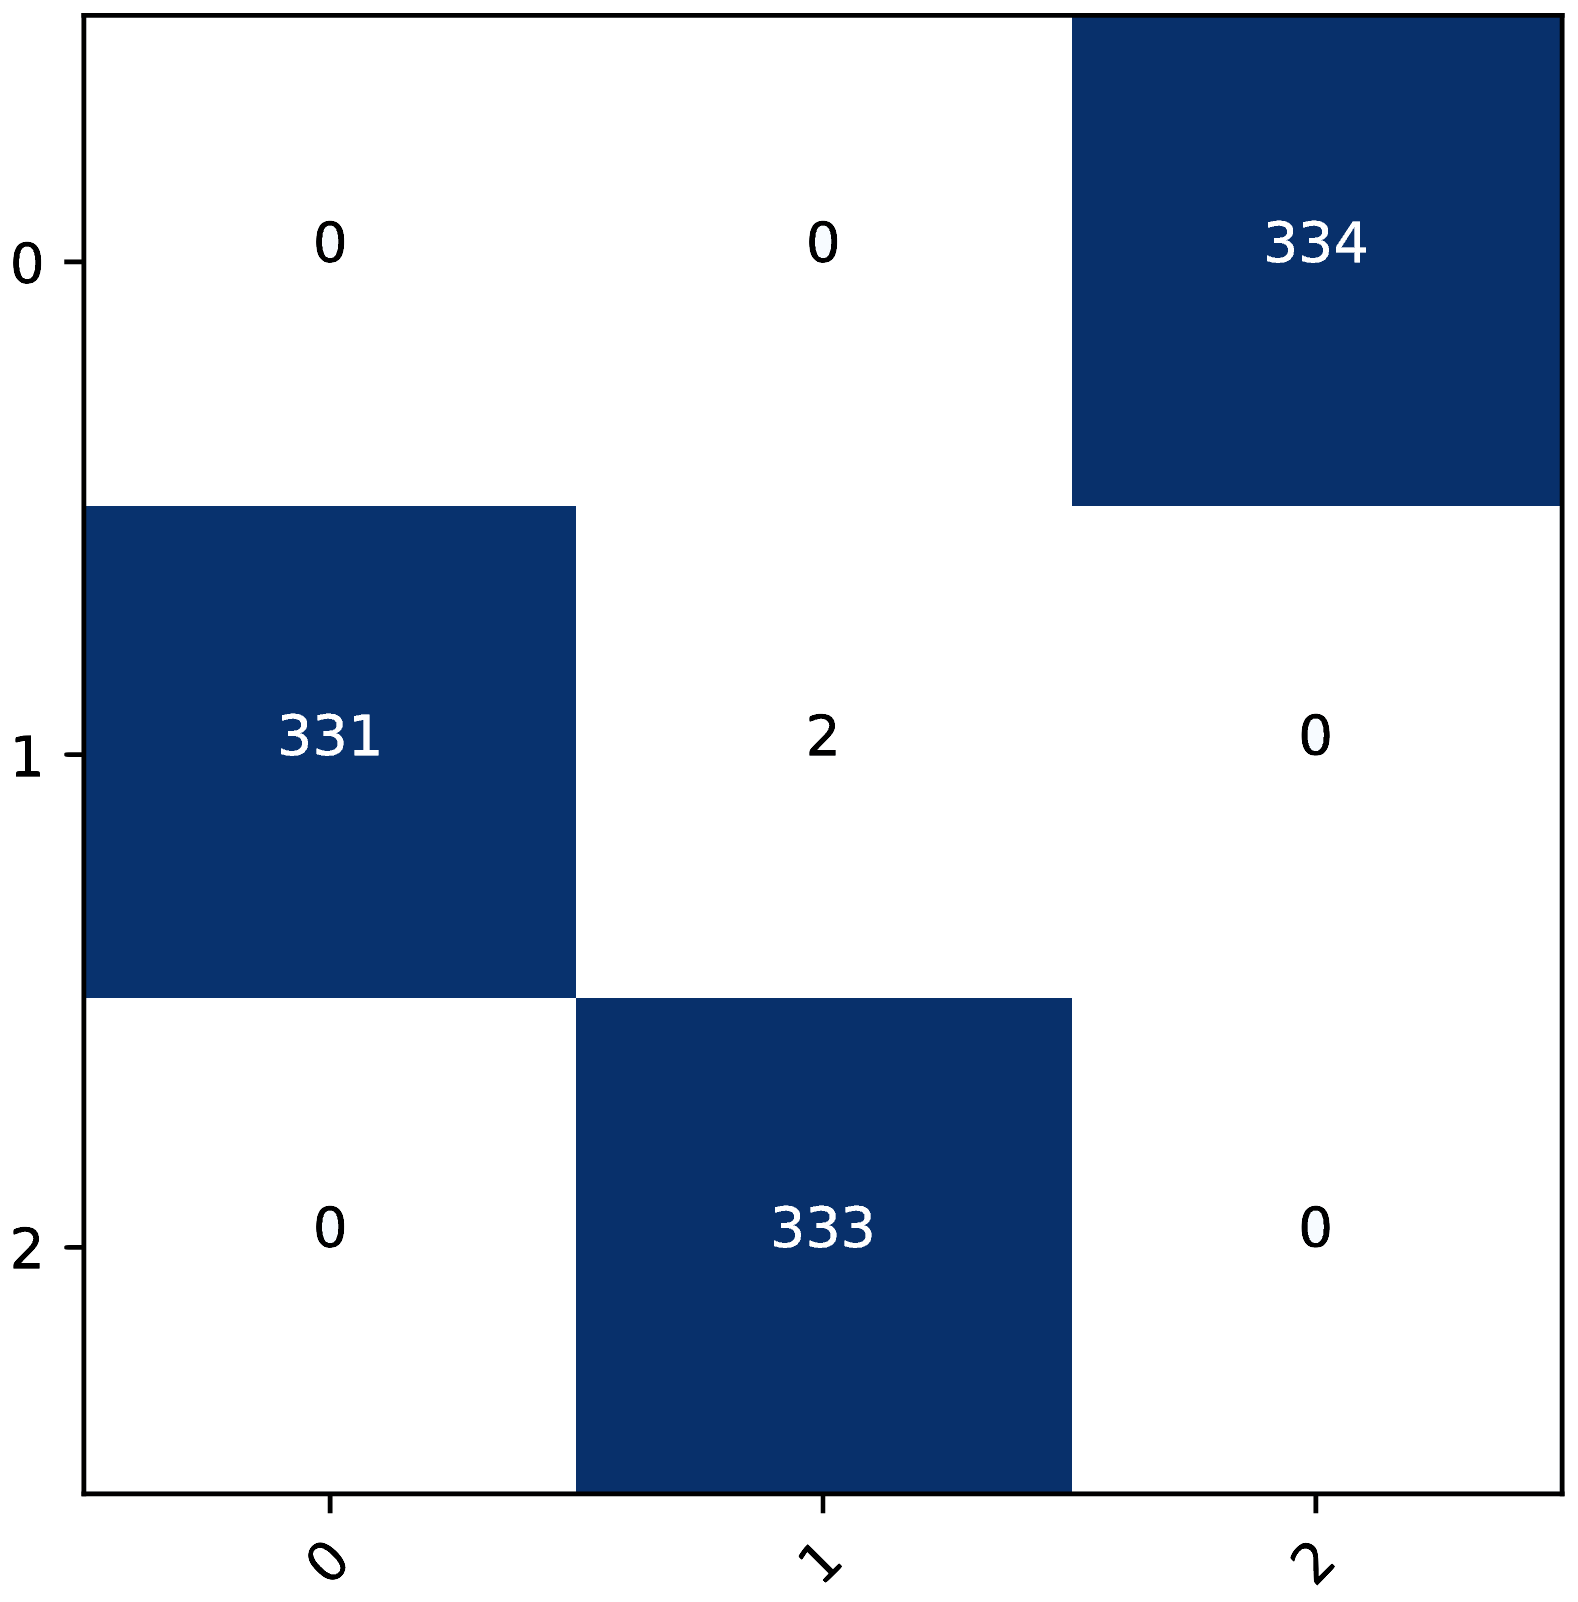
\includegraphics[height=.49\textheight, width=.99\textwidth, keepaspectratio]{blobs_confusion_matrix.png}
    \end{minipage}
    \begin{minipage}{.49\textwidth}
        \centering
        \setlength\figureheight{.65\textheight}
        \setlength\figurewidth{1.2\textwidth}
        % This file was created by matplotlib2tikz v0.6.11.
\begin{tikzpicture}

\definecolor{color1}{rgb}{1,0.498039215686275,0.0549019607843137}
\definecolor{color0}{rgb}{0.12156862745098,0.466666666666667,0.705882352941177}
\definecolor{color2}{rgb}{0.172549019607843,0.627450980392157,0.172549019607843}
\pgfplotsset{ticks=none}
\begin{axis}[
xmin=-0.0418216511537201, xmax=0.873761510375378,
ymin=-0.0472417465158804, ymax=0.983571673048558,
width=\figurewidth,
height=\figureheight,
tick pos=left
]
\addplot [only marks, mark size=0.5pt, draw=color0, fill=color0, colormap/viridis]
table{%
x                      y
+4.219231903553009e-01 +3.553238213062286e-01
+4.543713331222534e-01 +3.285980522632599e-01
+7.544563412666321e-01 +2.138124108314514e-01
+4.293923676013947e-01 +3.339084386825562e-01
+4.127488732337952e-01 +3.699249029159546e-01
+7.746628522872925e-01 +2.184964716434479e-01
+6.956143975257874e-01 +2.580470740795135e-01
+4.599608480930328e-01 +3.416456282138824e-01
+8.197553753852844e-01 +1.448495686054230e-01
+8.040107488632202e-01 +1.616706252098083e-01
+7.588247656822205e-01 +2.283389121294022e-01
+4.514042139053345e-01 +3.402256369590759e-01
+7.539239525794983e-01 +2.450002431869507e-01
+7.597731947898865e-01 +2.391263842582703e-01
+4.613696336746216e-01 +3.368245959281921e-01
+4.514349997043610e-01 +3.552212119102478e-01
+7.915121316909790e-01 +1.551029682159424e-01
+4.544831216335297e-01 +3.381157219409943e-01
+7.611153125762939e-01 +1.679451167583466e-01
+4.578820168972015e-01 +3.469123542308807e-01
+8.014632463455200e-01 +1.691008210182190e-01
+7.314484119415283e-01 +2.468717992305756e-01
+7.857026457786560e-01 +2.088068127632141e-01
+7.673105001449585e-01 +2.253431826829910e-01
+7.811254262924194e-01 +2.028274387121201e-01
+7.418822646141052e-01 +1.643714755773544e-01
+7.650328874588013e-01 +1.715147197246552e-01
+6.570470929145813e-01 +2.207997143268585e-01
+7.526094913482666e-01 +1.782444715499878e-01
+4.391746819019318e-01 +3.348402678966522e-01
+8.162030577659607e-01 +1.409313529729843e-01
+8.033780455589294e-01 +1.647261977195740e-01
+4.153328239917755e-01 +3.615469336509705e-01
+8.211663961410522e-01 +1.243981570005417e-01
+4.541591405868530e-01 +3.399068713188171e-01
+4.267233908176422e-01 +3.640479743480682e-01
+4.270552694797516e-01 +3.581504523754120e-01
+4.239512979984283e-01 +3.546443581581116e-01
+7.703629136085510e-01 +1.766041368246078e-01
+4.373623132705688e-01 +3.737907707691193e-01
+7.784012556076050e-01 +1.440441161394119e-01
+4.397125542163849e-01 +3.673625588417053e-01
+8.286561369895935e-01 +1.005793586373329e-01
+3.929725587368011e-01 +3.728328943252563e-01
+4.090956747531891e-01 +3.753848671913147e-01
+4.551824629306793e-01 +3.432158231735229e-01
+7.917047739028931e-01 +1.715743243694305e-01
+6.491242051124573e-01 +2.285328358411789e-01
+4.297766387462616e-01 +3.533477485179901e-01
+7.435912489891052e-01 +2.121741622686386e-01
+4.395152032375336e-01 +3.737236857414246e-01
+7.424215078353882e-01 +1.526210308074951e-01
+4.529505670070648e-01 +3.191524744033813e-01
+4.202068746089935e-01 +3.551334738731384e-01
+4.624554812908173e-01 +3.277458548545837e-01
+7.039268016815186e-01 +1.864966899156570e-01
+4.459904134273529e-01 +3.459074795246124e-01
+7.499038577079773e-01 +2.255477309226990e-01
+4.192264974117279e-01 +3.734280467033386e-01
+4.036251008510590e-01 +3.731558918952942e-01
+7.938987612724304e-01 +1.836477816104889e-01
+7.994005084037781e-01 +1.422469317913055e-01
+4.630206823348999e-01 +3.533456027507782e-01
+4.308787584304810e-01 +3.603324592113495e-01
+7.479857802391052e-01 +1.884034723043442e-01
+8.037795424461365e-01 +1.425065398216248e-01
+4.384578466415405e-01 +3.439678847789764e-01
+8.117547631263733e-01 +9.526474773883820e-02
+7.644836902618408e-01 +1.840516924858093e-01
+4.083176553249359e-01 +3.791846036911011e-01
+7.935335636138916e-01 +1.833828091621399e-01
+4.537455439567566e-01 +3.529103994369507e-01
+4.624099433422089e-01 +3.254284560680389e-01
+4.127783179283142e-01 +3.657649755477905e-01
+7.991129159927368e-01 +1.757124066352844e-01
+8.056054711341858e-01 +1.765022128820419e-01
+4.440854787826538e-01 +3.447553217411041e-01
+8.079522848129272e-01 +1.680098176002502e-01
+4.510765969753265e-01 +3.203281462192535e-01
+7.567164897918701e-01 +2.167893797159195e-01
+7.820181846618652e-01 +1.731999367475510e-01
+4.526980221271515e-01 +3.446747958660126e-01
+4.578627645969391e-01 +3.577384650707245e-01
+7.391865253448486e-01 +2.073835134506226e-01
+7.681884169578552e-01 +1.505558043718338e-01
+4.483594000339508e-01 +3.503434360027313e-01
+7.778313159942627e-01 +1.976983994245529e-01
+6.583015322685242e-01 +2.311744540929794e-01
+4.509860277175903e-01 +3.389677405357361e-01
+4.611359536647797e-01 +3.339437842369080e-01
+6.448860764503479e-01 +2.375031858682632e-01
+4.393452107906342e-01 +3.474427461624146e-01
+4.235661029815674e-01 +3.651033639907837e-01
+4.554707705974579e-01 +3.393692672252655e-01
+8.131560683250427e-01 +1.612922996282578e-01
+7.183142900466919e-01 +2.461485415697098e-01
+8.108548521995544e-01 +1.730003505945206e-01
+7.728241682052612e-01 +1.283218711614609e-01
+4.652241468429565e-01 +3.371395468711853e-01
+7.885581851005554e-01 +2.096385359764099e-01
+4.231189489364624e-01 +3.571663200855255e-01
+4.637693166732788e-01 +3.219909369945526e-01
+7.861025333404541e-01 +1.801749616861343e-01
+7.546318173408508e-01 +2.079087793827057e-01
+4.604453146457672e-01 +3.158225715160370e-01
+7.695235610008240e-01 +2.059553563594818e-01
+4.196191430091858e-01 +3.612008690834045e-01
+8.080803155899048e-01 +1.277569979429245e-01
+7.831879258155823e-01 +1.439173370599747e-01
+7.867820858955383e-01 +2.002982646226883e-01
+7.559465169906616e-01 +1.451874375343323e-01
+4.514401555061340e-01 +3.426514863967896e-01
+8.313751816749573e-01 +1.161234676837921e-01
+7.915825843811035e-01 +1.709175258874893e-01
+4.507459700107574e-01 +3.657163381576538e-01
+7.917891144752502e-01 +1.933166384696960e-01
+7.881387472152710e-01 +1.434485763311386e-01
+4.405604898929596e-01 +3.393384516239166e-01
+7.981696128845215e-01 +1.865579187870026e-01
+6.647185683250427e-01 +2.254313081502914e-01
+7.991232872009277e-01 +1.561251133680344e-01
+4.546393454074860e-01 +3.427581489086151e-01
+4.431634545326233e-01 +3.592935800552368e-01
+6.727302670478821e-01 +2.136905044317245e-01
+6.472663283348083e-01 +2.508238554000854e-01
+4.381307363510132e-01 +3.661230802536011e-01
+4.519313573837280e-01 +3.426666557788849e-01
+7.965516448020935e-01 +1.879852712154388e-01
+7.116366624832153e-01 +2.768019437789917e-01
+4.632619023323059e-01 +3.438836336135864e-01
+8.082023859024048e-01 +1.321274936199188e-01
+7.439301013946533e-01 +1.922256350517273e-01
+7.313275933265686e-01 +2.382559627294540e-01
+8.248165845870972e-01 +1.013746187090874e-01
+4.540366232395172e-01 +3.319545090198517e-01
+4.473024308681488e-01 +3.709026277065277e-01
+7.837905287742615e-01 +2.111917287111282e-01
+4.617385566234589e-01 +3.339883089065552e-01
+4.255863428115845e-01 +3.648313581943512e-01
+7.478035688400269e-01 +1.566240787506104e-01
+4.362286329269409e-01 +3.374400436878204e-01
+7.841978669166565e-01 +1.429377198219299e-01
+6.302680373191833e-01 +2.741584479808807e-01
+8.270103931427002e-01 +9.658815711736679e-02
+4.567679464817047e-01 +3.426627814769745e-01
+7.623980045318604e-01 +1.793117672204971e-01
+6.451767086982727e-01 +2.462099492549896e-01
+7.303239703178406e-01 +2.086174786090851e-01
+4.419365823268890e-01 +3.674243688583374e-01
+4.525919854640961e-01 +3.216820955276489e-01
+4.585800468921661e-01 +3.414892852306366e-01
+7.684960961341858e-01 +1.916397213935852e-01
+8.168586492538452e-01 +1.552322357892990e-01
+4.249027669429779e-01 +3.491778969764709e-01
+4.435535669326782e-01 +3.657649755477905e-01
+8.034669756889343e-01 +1.665926873683929e-01
+4.577280879020691e-01 +3.450700044631958e-01
+7.950469255447388e-01 +1.866798251867294e-01
+7.562716007232666e-01 +1.954404413700104e-01
+8.137825131416321e-01 +1.132334992289543e-01
+4.242616593837738e-01 +3.558768033981323e-01
+7.415206432342529e-01 +2.273584902286530e-01
+4.628178775310516e-01 +3.176156282424927e-01
+7.623800039291382e-01 +2.322259098291397e-01
+4.551163613796234e-01 +3.437117338180542e-01
+4.645319283008575e-01 +3.370590209960938e-01
+8.163750171661377e-01 +1.264037489891052e-01
+7.672508358955383e-01 +1.890566051006317e-01
+7.960005402565002e-01 +1.730660498142242e-01
+8.244198560714722e-01 +1.317415386438370e-01
+7.839782834053040e-01 +2.151286154985428e-01
+8.265539407730103e-01 +1.240768507122993e-01
+7.993574738502502e-01 +1.553639918565750e-01
+7.745826840400696e-01 +1.283607333898544e-01
+4.362970590591431e-01 +3.493767082691193e-01
+4.591065347194672e-01 +3.481217622756958e-01
+4.504088163375854e-01 +3.519860506057739e-01
+4.301033318042755e-01 +3.563877344131470e-01
+8.137809634208679e-01 +1.640865951776505e-01
+7.766677141189575e-01 +1.994920969009399e-01
+7.713037133216858e-01 +1.831294596195221e-01
+4.227917194366455e-01 +3.728091120719910e-01
+8.222199082374573e-01 +1.412677168846130e-01
+4.489284753799438e-01 +3.419508039951324e-01
+4.587124586105347e-01 +3.240734040737152e-01
+4.573542475700378e-01 +3.216585814952850e-01
+7.026672959327698e-01 +2.214658856391907e-01
+3.894180655479431e-01 +3.724009394645691e-01
+4.544753730297089e-01 +3.456597626209259e-01
+4.300346672534943e-01 +3.616222739219666e-01
+7.885259389877319e-01 +1.748391985893250e-01
+4.532519578933716e-01 +3.359733223915100e-01
+6.480589509010315e-01 +2.374463230371475e-01
+7.720413804054260e-01 +1.847837567329407e-01
+7.532727718353271e-01 +2.464956343173981e-01
+4.447888433933258e-01 +3.248409330844879e-01
+4.307785332202911e-01 +3.704055547714233e-01
+4.457956552505493e-01 +3.500294089317322e-01
+8.257301449775696e-01 +1.276407092809677e-01
+7.147015333175659e-01 +2.340774685144424e-01
+4.561573266983032e-01 +3.531147241592407e-01
+4.629656076431274e-01 +3.257733285427094e-01
+7.668464779853821e-01 +2.009981572628021e-01
+4.442100822925568e-01 +3.641687333583832e-01
+4.627491831779480e-01 +3.276826143264771e-01
+7.915261983871460e-01 +2.043348550796509e-01
+7.633138895034790e-01 +1.943187117576599e-01
+4.567326605319977e-01 +3.454301357269287e-01
+4.427555501461029e-01 +3.319662809371948e-01
+4.387689828872681e-01 +3.528021574020386e-01
+7.940902113914490e-01 +1.739149987697601e-01
+8.003842830657959e-01 +1.851196140050888e-01
+4.441119134426117e-01 +3.523678183555603e-01
+7.552592754364014e-01 +2.020166367292404e-01
+4.500264227390289e-01 +3.475435674190521e-01
+7.803657650947571e-01 +1.835778206586838e-01
+7.450301647186279e-01 +2.445163577795029e-01
+8.118895888328552e-01 +1.287975460290909e-01
+4.335364401340485e-01 +3.233186006546021e-01
+4.596376717090607e-01 +3.416370749473572e-01
+8.150993585586548e-01 +1.513558030128479e-01
+4.475199580192566e-01 +3.507750332355499e-01
+8.162842392921448e-01 +1.382846981287003e-01
+4.164161980152130e-01 +3.681503534317017e-01
+7.894371151924133e-01 +1.488702297210693e-01
+4.669414758682251e-01 +3.324049711227417e-01
+7.212857007980347e-01 +2.766298949718475e-01
+4.464250802993774e-01 +3.349609076976776e-01
+8.220062851905823e-01 +1.418216675519943e-01
+4.499966800212860e-01 +3.561517000198364e-01
+4.207778275012970e-01 +3.447337448596954e-01
+7.287070751190186e-01 +1.901581883430481e-01
+4.387525320053101e-01 +3.632086515426636e-01
+7.490108609199524e-01 +2.286802828311920e-01
+7.836616635322571e-01 +2.079389989376068e-01
+4.550818502902985e-01 +3.419798612594604e-01
+8.086801171302795e-01 +7.152258604764938e-02
+7.336242198944092e-01 +1.411426216363907e-01
+4.385150671005249e-01 +3.664440214633942e-01
+6.924557685852051e-01 +2.198004126548767e-01
+4.361343085765839e-01 +3.368831276893616e-01
+8.021698594093323e-01 +1.495044678449631e-01
+3.894436955451965e-01 +3.817599415779114e-01
+4.492416679859161e-01 +3.499121367931366e-01
+4.308904707431793e-01 +3.491283655166626e-01
+8.046394586563110e-01 +1.022239774465561e-01
+4.182218909263611e-01 +3.496423661708832e-01
+7.205193042755127e-01 +2.793945670127869e-01
+4.558566808700562e-01 +3.397937119007111e-01
+4.403394460678101e-01 +3.376463651657104e-01
+4.529217481613159e-01 +3.465021550655365e-01
+7.999091148376465e-01 +1.545228511095047e-01
+7.952476739883423e-01 +1.151393130421638e-01
+6.518105864524841e-01 +2.302088290452957e-01
+3.988166749477386e-01 +3.775192499160767e-01
+4.594144523143768e-01 +3.305929899215698e-01
+4.571955502033234e-01 +3.434716463088989e-01
+7.922468781471252e-01 +1.201403737068176e-01
+8.110658526420593e-01 +1.342429518699646e-01
+4.336281120777130e-01 +3.576380014419556e-01
+4.229351282119751e-01 +3.589731454849243e-01
+8.208925724029541e-01 +1.471020877361298e-01
+8.058235049247742e-01 +1.392891556024551e-01
+4.546405076980591e-01 +3.503319919109344e-01
+4.445825517177582e-01 +3.548376560211182e-01
+4.365016818046570e-01 +3.456001579761505e-01
+4.393831193447113e-01 +3.583259284496307e-01
+7.763291001319885e-01 +2.070140689611435e-01
+4.505296945571899e-01 +3.465609848499298e-01
+8.117874860763550e-01 +1.704243421554565e-01
+4.095763266086578e-01 +3.694292008876801e-01
+7.444490194320679e-01 +1.960269957780838e-01
+4.095283150672913e-01 +3.554301857948303e-01
+7.643889784812927e-01 +1.949283778667450e-01
+8.123472332954407e-01 +1.678636223077774e-01
+7.385762929916382e-01 +1.707040965557098e-01
+7.690606713294983e-01 +2.018031924962997e-01
+7.807014584541321e-01 +2.115518450737000e-01
+7.622682452201843e-01 +1.964467465877533e-01
+7.360196709632874e-01 +1.681327223777771e-01
+4.651223123073578e-01 +3.363302946090698e-01
+7.742995619773865e-01 +1.654024720191956e-01
+4.366964101791382e-01 +3.432689011096954e-01
+7.874349355697632e-01 +1.793510019779205e-01
+4.665820300579071e-01 +3.104020059108734e-01
+4.466251134872437e-01 +3.354412317276001e-01
+8.186490535736084e-01 +1.402728408575058e-01
+3.946034312248230e-01 +3.891929388046265e-01
+4.207774698734283e-01 +3.640530705451965e-01
+4.501536190509796e-01 +3.466314375400543e-01
+7.508575320243835e-01 +2.175610512495041e-01
+7.767173647880554e-01 +2.176088690757751e-01
+4.436416923999786e-01 +3.349376916885376e-01
+6.393663883209229e-01 +2.557812035083771e-01
+8.130029439926147e-01 +1.322431713342667e-01
+4.435997307300568e-01 +3.560715019702911e-01
+4.482075870037079e-01 +3.355902433395386e-01
+4.650789499282837e-01 +3.247834444046021e-01
+7.793505191802979e-01 +2.013778835535049e-01
+7.433122992515564e-01 +2.277067303657532e-01
+4.362986385822296e-01 +3.461855351924896e-01
+4.418117105960846e-01 +3.517642319202423e-01
+8.314979076385498e-01 +6.999836862087250e-02
+4.596099555492401e-01 +3.387274146080017e-01
+4.217847883701324e-01 +3.793445825576782e-01
+4.421694874763489e-01 +3.714087307453156e-01
+8.077471256256104e-01 +1.680906414985657e-01
+6.728441715240479e-01 +2.436315119266510e-01
+4.627268910408020e-01 +3.561512231826782e-01
+7.532035708427429e-01 +2.449434697628021e-01
+8.318253159523010e-01 +6.524097174406052e-02
+4.606933891773224e-01 +3.370496332645416e-01
+6.640888452529907e-01 +2.599830925464630e-01
+7.930900454521179e-01 +1.794382929801941e-01
+4.078903496265411e-01 +3.763072192668915e-01
+4.214489459991455e-01 +3.501382172107697e-01
+4.351247549057007e-01 +3.647787868976593e-01
+7.597076296806335e-01 +2.101955264806747e-01
+4.410549402236938e-01 +3.671400845050812e-01
+4.317920804023743e-01 +3.547245264053345e-01
+8.102363348007202e-01 +1.006365790963173e-01
+4.217303395271301e-01 +3.411063849925995e-01
+4.152144193649292e-01 +3.855022490024567e-01
+7.568231225013733e-01 +2.063794881105423e-01
+7.381948232650757e-01 +2.351323962211609e-01
+4.569774866104126e-01 +3.422299921512604e-01
+7.024562954902649e-01 +2.245916873216629e-01
+7.164611220359802e-01 +2.265070527791977e-01
+7.419206500053406e-01 +1.795361638069153e-01
+4.575167596340179e-01 +3.371214270591736e-01
+7.452079057693481e-01 +2.066942155361176e-01
};
\addplot [only marks, mark size=0.5pt, draw=color1, fill=color1, colormap/viridis]
table{%
x                      y
+1.581830978393555e-01 +7.520376443862915e-01
+1.783129870891571e-01 +7.638176083564758e-01
+1.130266264081001e-01 +7.909346222877502e-01
+1.057442724704742e-01 +7.848440408706665e-01
+1.376734375953674e-01 +7.266345024108887e-01
+1.468250900506973e-01 +7.613780498504639e-01
+1.329507231712341e-01 +7.399520874023438e-01
+1.644477248191833e-01 +7.986060976982117e-01
+6.412649899721146e-02 +8.763177394866943e-01
+1.807100474834442e-01 +7.335663437843323e-01
+7.868299633264542e-02 +8.062948584556580e-01
+1.305291652679443e-01 +7.603480815887451e-01
+9.753960371017456e-02 +8.237459659576416e-01
+9.731234610080719e-02 +7.750397324562073e-01
+1.337831169366837e-01 +7.564011216163635e-01
+2.117597460746765e-01 +7.881395816802979e-01
+1.441366374492645e-01 +7.509154677391052e-01
+8.873525261878967e-02 +8.277658224105835e-01
+1.450478881597519e-01 +7.922644019126892e-01
+1.425831019878387e-01 +7.710497379302979e-01
+6.239417940378189e-02 +8.604202866554260e-01
+5.090526491403580e-02 +8.216779828071594e-01
+3.249185159802437e-02 +8.983915448188782e-01
+1.353454589843750e-01 +7.668868303298950e-01
+1.152838915586472e-01 +7.850416302680969e-01
+8.755877614021301e-02 +7.554754614830017e-01
+6.515360623598099e-02 +8.579892516136169e-01
+1.021547541022301e-01 +7.821663022041321e-01
+1.098698675632477e-01 +8.100196719169617e-01
+1.069113239645958e-01 +8.302260041236877e-01
+1.243197470903397e-01 +7.480690479278564e-01
+4.970217123627663e-02 +8.312309384346008e-01
+1.063769981265068e-01 +7.960306406021118e-01
+1.796768903732300e-01 +6.941223144531250e-01
+1.497278362512589e-01 +8.231223225593567e-01
+4.904459789395332e-02 +8.937169909477234e-01
+1.397809833288193e-01 +8.165975809097290e-01
+2.554766833782196e-02 +9.365636706352234e-01
+1.439761966466904e-01 +8.481875061988831e-01
+7.617772370576859e-02 +8.310977220535278e-01
+1.402158588171005e-01 +7.548573017120361e-01
+9.016574919223785e-02 +8.926723599433899e-01
+1.301794648170471e-01 +8.001223206520081e-01
+6.917811185121536e-02 +7.907493710517883e-01
+1.522796005010605e-01 +8.254545331001282e-01
+1.117360219359398e-01 +7.858282327651978e-01
+1.087922826409340e-01 +8.110399842262268e-01
+9.739552438259125e-02 +8.565618991851807e-01
+8.200272917747498e-02 +7.745406627655029e-01
+1.004800722002983e-01 +8.290550112724304e-01
+1.366370171308517e-01 +7.923666238784790e-01
+6.322434544563293e-02 +8.150357604026794e-01
+1.115874350070953e-01 +7.770666480064392e-01
+1.145502775907516e-01 +7.826006412506104e-01
+1.171877607703209e-01 +7.713854312896729e-01
+1.153087839484215e-01 +8.132637143135071e-01
+2.817503176629543e-02 +8.849408626556396e-01
+4.977602884173393e-02 +8.425134420394897e-01
+1.729773879051208e-01 +7.995828390121460e-01
+1.436989009380341e-01 +7.909849286079407e-01
+6.542018800973892e-02 +8.086631298065186e-01
+9.091990441083908e-02 +7.826285362243652e-01
+3.565255403518677e-01 +3.999239802360535e-01
+4.406352341175079e-02 +8.346329331398010e-01
+1.107158586382866e-01 +8.386228680610657e-01
+1.135140359401703e-01 +8.318487405776978e-01
+1.222496107220650e-01 +8.440476059913635e-01
+2.023359239101410e-01 +7.379752397537231e-01
+1.409578919410706e-01 +7.546188235282898e-01
+1.460389494895935e-01 +7.742508649826050e-01
+1.899660527706146e-01 +7.209423184394836e-01
+1.166343763470650e-01 +8.486992716789246e-01
+1.753130853176117e-01 +7.933069467544556e-01
+5.079155787825584e-02 +8.416568040847778e-01
+3.673742711544037e-02 +9.110210537910461e-01
+7.264722138643265e-02 +8.472747206687927e-01
+5.012386664748192e-02 +9.142379164695740e-01
+8.972297608852386e-02 +7.894361019134521e-01
+2.519811391830444e-01 +7.472641468048096e-01
+7.894554734230042e-02 +8.667367696762085e-01
+8.865873515605927e-02 +8.452399373054504e-01
+1.664791256189346e-01 +7.810492515563965e-01
+5.899905785918236e-02 +8.593112826347351e-01
+9.327848255634308e-02 +8.108111023902893e-01
+6.613448262214661e-02 +8.241042494773865e-01
+1.234089657664299e-01 +7.892234921455383e-01
+5.649835988879204e-02 +8.241355419158936e-01
+1.544466465711594e-01 +8.029527068138123e-01
+1.711768954992294e-01 +7.755233049392700e-01
+2.710776627063751e-01 +7.170265913009644e-01
+8.771041035652161e-02 +8.076247572898865e-01
+1.301295310258865e-01 +7.652080059051514e-01
+1.692402660846710e-01 +7.238039970397949e-01
+1.244116425514221e-01 +7.984208464622498e-01
+1.385996043682098e-01 +7.882530093193054e-01
+1.275637000799179e-01 +7.878295779228210e-01
+1.228669541887939e-03 +9.322428107261658e-01
+2.018276281887665e-04 +8.979976773262024e-01
+1.246766299009323e-01 +8.019660711288452e-01
+8.236322551965714e-02 +8.355177044868469e-01
+2.966187149286270e-02 +8.942010998725891e-01
+1.322300285100937e-01 +7.634576559066772e-01
+3.093594126403332e-02 +8.470084667205811e-01
+8.998499810695648e-02 +8.054503798484802e-01
+9.503512992523611e-04 +9.263741970062256e-01
+6.407784670591354e-02 +8.508988022804260e-01
+3.680588304996490e-02 +8.190206885337830e-01
+9.222373366355896e-02 +8.250425457954407e-01
+1.532744765281677e-01 +7.703170180320740e-01
+5.048484727740288e-02 +8.648660182952881e-01
+1.170428469777107e-01 +7.672339677810669e-01
+2.364716678857803e-01 +7.628829479217529e-01
+6.565714627504349e-02 +8.193051815032959e-01
+8.834370970726013e-02 +8.867008686065674e-01
+8.877808600664139e-02 +7.743964195251465e-01
+1.407620608806610e-01 +7.864524722099304e-01
+9.428539127111435e-02 +7.959358096122742e-01
+7.269773632287979e-02 +8.104864358901978e-01
+1.014210730791092e-01 +7.794900536537170e-01
+1.107066050171852e-01 +8.264945745468140e-01
+7.883873581886292e-02 +8.035919070243835e-01
+1.642238795757294e-01 +8.102059960365295e-01
+1.311397403478622e-01 +7.751539349555969e-01
+2.743378877639771e-01 +7.241364121437073e-01
+7.532738894224167e-02 +8.036420345306396e-01
+1.000591292977333e-01 +8.023399114608765e-01
+1.031309962272644e-01 +7.685043811798096e-01
+1.250972151756287e-01 +7.774916887283325e-01
+7.453737407922745e-02 +8.847809433937073e-01
+1.347952634096146e-01 +8.087896704673767e-01
+7.940385490655899e-02 +8.574594259262085e-01
+6.038527190685272e-02 +8.692397475242615e-01
+1.016842871904373e-01 +8.418800830841064e-01
+8.062065392732620e-02 +7.927545309066772e-01
+1.397297680377960e-01 +7.498498558998108e-01
+6.068166717886925e-02 +8.246917724609375e-01
+1.128435041755438e-02 +8.822166919708252e-01
+1.150998845696449e-01 +7.998344302177429e-01
+1.014436632394791e-01 +8.745368719100952e-01
+5.118084326386452e-02 +8.772814273834229e-01
+1.522025913000107e-01 +7.877303361892700e-01
+1.445877104997635e-01 +7.847138047218323e-01
+1.376830186927691e-04 +8.982875347137451e-01
+9.206612408161163e-02 +8.752052783966064e-01
+1.084238439798355e-01 +7.942436337471008e-01
+1.092671677470207e-01 +8.048242330551147e-01
+1.298195719718933e-01 +7.603123188018799e-01
+1.052293702960014e-01 +7.557857036590576e-01
+4.477924853563309e-02 +8.463661670684814e-01
+1.596803516149521e-01 +8.402886390686035e-01
+1.602153927087784e-01 +7.931054830551147e-01
+1.439063400030136e-01 +7.977980971336365e-01
+7.957780361175537e-02 +8.434857726097107e-01
+1.778486073017120e-01 +7.598770260810852e-01
+1.164944842457771e-01 +8.155136704444885e-01
+1.136169359087944e-01 +7.642288804054260e-01
+1.633339524269104e-01 +7.850496172904968e-01
+1.138067319989204e-01 +8.045912384986877e-01
+9.856786578893661e-02 +7.917708754539490e-01
+1.975515335798264e-01 +7.425130605697632e-01
+7.157001644372940e-02 +8.214415907859802e-01
+1.016117259860039e-01 +8.191610574722290e-01
+1.210727617144585e-01 +8.461865782737732e-01
+1.109921634197235e-01 +8.138038516044617e-01
+9.512290358543396e-02 +7.921531796455383e-01
+1.260605603456497e-01 +8.236391544342041e-01
+1.114673689007759e-01 +7.756398916244507e-01
+9.573557227849960e-02 +8.175378441810608e-01
+5.941728129982948e-02 +8.773781657218933e-01
+1.414721161127090e-01 +7.812829017639160e-01
+1.409329771995544e-01 +7.461235523223877e-01
+5.209587886929512e-02 +9.032598137855530e-01
+8.192764967679977e-02 +7.936601042747498e-01
+6.146670505404472e-02 +8.451157212257385e-01
+1.641444563865662e-01 +7.430190443992615e-01
+6.473717838525772e-02 +8.962249159812927e-01
+5.792554467916489e-02 +9.163153171539307e-01
+5.045480281114578e-02 +8.781278133392334e-01
+1.543217152357101e-01 +7.873357534408569e-01
+7.218075543642044e-02 +8.475499749183655e-01
+2.163831144571304e-01 +7.835685610771179e-01
+8.950230479240417e-02 +8.176597356796265e-01
+1.136469747871161e-02 +9.049384593963623e-01
+8.176029473543167e-02 +8.150407671928406e-01
+1.616058945655823e-01 +7.629778385162354e-01
+1.366236507892609e-01 +8.006333112716675e-01
+1.301727145910263e-01 +7.439956068992615e-01
+1.312274783849716e-01 +8.410726785659790e-01
+9.144455939531326e-02 +7.968163490295410e-01
+2.833056636154652e-02 +9.239037036895752e-01
+1.057628169655800e-01 +7.957106828689575e-01
+4.986605793237686e-02 +8.827583789825439e-01
+1.513277646154165e-02 +8.718717098236084e-01
+7.161559909582138e-02 +8.106564879417419e-01
+9.776172786951065e-02 +8.126604557037354e-01
+1.562347263097763e-01 +8.174514174461365e-01
+1.118815913796425e-01 +7.890998721122742e-01
+8.264203369617462e-02 +8.034292459487915e-01
+4.308577999472618e-02 +9.155986309051514e-01
+1.729744970798492e-01 +7.375156879425049e-01
+6.023228168487549e-02 +8.499172329902649e-01
+4.521675407886505e-02 +8.632810115814209e-01
+8.923056721687317e-02 +8.907698988914490e-01
+1.493826508522034e-01 +7.936677336692810e-01
+1.504447311162949e-01 +8.028516173362732e-01
+6.790732592344284e-02 +8.606261610984802e-01
+9.005101025104523e-02 +7.908600568771362e-01
+9.573873877525330e-02 +8.274767398834229e-01
+8.378973603248596e-02 +8.600410223007202e-01
+8.537830412387848e-02 +8.283684253692627e-01
+4.102855455130339e-03 +9.296410083770752e-01
+1.278419345617294e-01 +8.211546540260315e-01
+8.191548287868500e-02 +8.119305968284607e-01
+1.213331446051598e-01 +7.989885807037354e-01
+5.313045531511307e-02 +8.916161060333252e-01
+8.703421801328659e-02 +8.960421085357666e-01
+1.498701572418213e-01 +7.490003705024719e-01
+1.294000297784805e-01 +7.891815304756165e-01
+1.304552406072617e-01 +7.632319927215576e-01
+9.186306595802307e-02 +8.345258831977844e-01
+9.182587265968323e-02 +8.679836988449097e-01
+4.851103201508522e-02 +8.231324553489685e-01
+9.007613360881805e-02 +8.050643205642700e-01
+1.577894538640976e-01 +7.987694740295410e-01
+1.629817634820938e-01 +7.817222476005554e-01
+1.307564377784729e-01 +7.652863264083862e-01
+1.269127875566483e-01 +7.811331748962402e-01
+7.207158207893372e-02 +8.349656462669373e-01
+6.274163722991943e-02 +8.362303376197815e-01
+7.191170752048492e-02 +7.884750962257385e-01
+1.192171648144722e-01 +7.830376625061035e-01
+3.374792635440826e-02 +8.949024677276611e-01
+7.830382138490677e-02 +8.345440626144409e-01
+8.617400377988815e-02 +8.350955247879028e-01
+1.128388121724129e-01 +7.927268743515015e-01
+1.067485883831978e-01 +8.330361247062683e-01
+7.838293095119298e-05 +8.831870555877686e-01
+1.409222781658173e-01 +7.461580038070679e-01
+1.007951572537422e-01 +7.921142578125000e-01
+7.376015931367874e-02 +8.510895371437073e-01
+1.480093002319336e-01 +8.011528253555298e-01
+8.809810876846313e-02 +8.402504920959473e-01
+7.888544350862503e-02 +8.331838846206665e-01
+8.915962278842926e-02 +8.149635195732117e-01
+1.361866593360901e-01 +7.627157568931580e-01
+1.049555763602257e-01 +8.324660658836365e-01
+1.108912527561188e-01 +7.975924015045166e-01
+4.383184015750885e-02 +8.745597600936890e-01
+2.182649821043015e-01 +7.815544009208679e-01
+1.596593707799911e-01 +8.402611613273621e-01
+9.590309113264084e-02 +8.212363719940186e-01
+1.784689128398895e-01 +7.385970950126648e-01
+2.909731678664684e-02 +8.949716687202454e-01
+7.044517248868942e-02 +8.167367577552795e-01
+1.357185691595078e-01 +7.844594717025757e-01
+3.797580301761627e-02 +8.667854070663452e-01
+3.598808869719505e-02 +8.950498104095459e-01
+1.342389285564423e-01 +7.906693220138550e-01
+6.600079685449600e-02 +8.022865056991577e-01
+3.883196040987968e-02 +8.883311748504639e-01
+1.119244992733002e-01 +7.950263023376465e-01
+7.111075520515442e-02 +8.285265564918518e-01
+1.246900781989098e-01 +8.092263936996460e-01
+6.762944906949997e-02 +9.312202930450439e-01
+6.408485770225525e-02 +8.400753736495972e-01
+1.334314942359924e-01 +7.985635995864868e-01
+1.771101914346218e-02 +9.248808026313782e-01
+2.011000961065292e-01 +7.986932396888733e-01
+1.052844077348709e-01 +7.868779897689819e-01
+1.330460757017136e-01 +7.579354047775269e-01
+1.100852191448212e-01 +7.477945089340210e-01
+1.002155393362045e-01 +7.848333120346069e-01
+6.221163645386696e-02 +8.102517724037170e-01
+1.205596998333931e-01 +7.723586559295654e-01
+7.008899003267288e-02 +8.695604205131531e-01
+3.796173036098480e-01 +3.859657347202301e-01
+9.585800766944885e-02 +7.718378305435181e-01
+1.307966560125351e-01 +7.702942490577698e-01
+1.060622185468674e-01 +8.506345152854919e-01
+1.077096015214920e-01 +8.143007755279541e-01
+1.395757347345352e-01 +7.369811534881592e-01
+1.198298931121826e-01 +7.688782215118408e-01
+5.698906257748604e-02 +8.585254549980164e-01
+8.272032439708710e-02 +8.741537332534790e-01
+1.452615112066269e-01 +7.725517153739929e-01
+1.069771945476532e-01 +8.175787329673767e-01
+1.903399825096130e-01 +7.416337728500366e-01
+1.486348509788513e-01 +8.001731634140015e-01
+1.610640883445740e-01 +7.658156752586365e-01
+5.632114782929420e-02 +8.519620299339294e-01
+1.267264485359192e-01 +7.918349504470825e-01
+1.175406053662300e-01 +7.652212381362915e-01
+1.422357559204102e-01 +8.577221035957336e-01
+2.400930821895599e-01 +7.474029660224915e-01
+3.442137688398361e-02 +8.993830084800720e-01
+9.751978516578674e-02 +7.971199154853821e-01
+1.454270035028458e-01 +8.076272606849670e-01
+5.551861226558685e-02 +8.225013613700867e-01
+1.758708357810974e-01 +7.306821942329407e-01
+1.298596411943436e-01 +7.697601914405823e-01
+6.132033839821815e-02 +8.650060892105103e-01
+2.929566614329815e-02 +9.075219631195068e-01
+9.215958416461945e-02 +8.126901388168335e-01
+1.459770351648331e-01 +7.854055166244507e-01
+1.427612453699112e-01 +8.121183514595032e-01
+1.497137546539307e-01 +7.710754871368408e-01
+9.526024013757706e-02 +8.075074553489685e-01
+7.200051099061966e-02 +7.588400244712830e-01
+1.804230511188507e-01 +7.800796031951904e-01
+5.150751769542694e-02 +8.673269748687744e-01
+1.385652720928192e-01 +7.287665605545044e-01
+1.625831276178360e-01 +7.735244631767273e-01
+9.114988148212433e-02 +8.190918564796448e-01
+1.245329827070236e-01 +7.694557309150696e-01
+1.895644068717957e-01 +7.693355083465576e-01
+6.367877125740051e-02 +8.810271620750427e-01
+3.273010626435280e-02 +8.683041334152222e-01
+1.163704693317413e-01 +7.935025691986084e-01
+1.592512577772141e-01 +7.630073428153992e-01
+4.411744698882103e-02 +8.872529864311218e-01
+1.485547423362732e-01 +8.513495922088623e-01
+9.711493551731110e-02 +8.282541036605835e-01
+1.717898547649384e-01 +7.806168198585510e-01
+1.811287701129913e-01 +7.748954296112061e-01
+8.418883383274078e-02 +8.545102477073669e-01
+6.256625056266785e-02 +8.551782965660095e-01
+3.599167242646217e-02 +8.701179027557373e-01
+1.043926402926445e-01 +7.575675249099731e-01
+8.757073432207108e-02 +8.329390883445740e-01
+9.701576828956604e-02 +8.324715495109558e-01
+2.137099765241146e-02 +8.663351535797119e-01
+1.265955716371536e-01 +8.520708680152893e-01
+1.159715726971626e-01 +7.842031717300415e-01
+1.625499129295349e-01 +7.684372663497925e-01
+1.130349412560463e-01 +8.206611871719360e-01
};
\addplot [only marks, mark size=0.5pt, draw=color2, fill=color2, colormap/viridis]
table{%
x                      y
+1.190802305936813e-01 +9.348866343498230e-02
+7.343520969152451e-02 +1.503972016507760e-04
+3.154235705733299e-02 +1.016702577471733e-01
+1.098003312945366e-01 +8.265315741300583e-02
+7.864055782556534e-02 +7.202469557523727e-02
+8.509626239538193e-02 +3.147776052355766e-02
+5.587529018521309e-02 +6.951188296079636e-02
+5.962232127785683e-02 +8.067189902067184e-02
+6.224238499999046e-02 +6.156193837523460e-02
+1.017025932669640e-01 +8.062983304262161e-02
+3.077338263392448e-02 +9.940852224826813e-02
+6.756053864955902e-02 +6.005288287997246e-02
+7.421160489320755e-02 +8.284054696559906e-02
+9.472789615392685e-02 +7.215737551450729e-02
+1.269009113311768e-01 +5.304986611008644e-02
+5.394427850842476e-02 +1.107671037316322e-01
+1.429881900548935e-01 +4.238176718354225e-02
+1.265687197446823e-01 +6.265787035226822e-02
+7.802537083625793e-02 +1.055155470967293e-01
+6.511784344911575e-02 +7.672879099845886e-02
+9.115157276391983e-02 +9.202585369348526e-02
+9.751376509666443e-02 +9.550342708826065e-02
+5.089710652828217e-02 +1.071014627814293e-01
+9.980333596467972e-02 +4.342109337449074e-02
+9.777352213859558e-02 +3.865748271346092e-02
+7.094848901033401e-02 +1.168347075581551e-01
+1.156498491764069e-01 +4.012800753116608e-02
+1.700430661439896e-01 +4.248506575822830e-02
+7.860317826271057e-02 +1.226310133934021e-01
+1.315501183271408e-01 +1.652625016868114e-02
+1.402053236961365e-01 +5.378297343850136e-02
+6.689321249723434e-02 +9.738571196794510e-02
+9.766490757465363e-02 +1.234921813011169e-01
+9.025964140892029e-02 +7.511374354362488e-02
+1.160736009478569e-01 +4.424540698528290e-02
+8.429802209138870e-02 +9.415338188409805e-02
+9.162244200706482e-02 +6.601432710886002e-02
+6.408273428678513e-02 +9.847832471132278e-02
+6.213473901152611e-02 +4.041101038455963e-02
+6.461033970117569e-02 +1.275673061609268e-01
+1.165759488940239e-01 +8.843386918306351e-02
+1.459246277809143e-01 +3.539204970002174e-02
+1.955520920455456e-02 +1.511287838220596e-01
+3.922432661056519e-02 +1.404981762170792e-01
+9.515323489904404e-02 +1.465813964605331e-01
+4.497368633747101e-02 +9.759171307086945e-02
+6.843174993991852e-02 +9.093579649925232e-02
+1.693890392780304e-01 +1.653064042329788e-02
+9.849261492490768e-02 +6.532812863588333e-02
+4.963968694210052e-02 +1.011934354901314e-01
+1.940905489027500e-02 +1.004044562578201e-01
+1.141032949090004e-01 +1.962649635970592e-02
+2.203692048788071e-01 +2.370660695305560e-05
+1.199073046445847e-01 +5.682085826992989e-02
+6.914673745632172e-02 +5.689731985330582e-02
+9.815397113561630e-02 +1.296246498823166e-01
+6.732078641653061e-02 +1.053880378603935e-01
+1.102164834737778e-01 +4.721592366695404e-02
+8.035942912101746e-02 +9.777068346738815e-02
+3.224641084671021e-02 +8.136462420225143e-02
+5.972481891512871e-02 +7.012701779603958e-02
+1.184329316020012e-01 +6.600574404001236e-02
+1.069069653749466e-01 +1.102368459105492e-01
+7.708739489316940e-02 +1.228988170623779e-01
+8.772372454404831e-02 +5.210494622588158e-02
+1.084302514791489e-01 +9.669198840856552e-02
+8.884852379560471e-02 +1.009231656789780e-01
+8.904020488262177e-02 +1.126321330666542e-01
+7.566546648740768e-02 +9.839503467082977e-02
+3.727388009428978e-02 +1.199684813618660e-01
+7.378052920103073e-02 +7.913220673799515e-02
+2.555158175528049e-02 +1.373634934425354e-01
+1.240441352128983e-01 +7.957461476325989e-02
+1.476170867681503e-01 +3.528546914458275e-02
+1.330020576715469e-01 +2.054552023764700e-04
+9.152548760175705e-02 +4.311895743012428e-02
+1.116972863674164e-01 +9.349480271339417e-02
+7.830712199211121e-02 +5.954328924417496e-02
+1.488569229841232e-01 +5.604470893740654e-02
+1.087729539722204e-02 +1.526648849248886e-01
+6.195100769400597e-02 +1.103474795818329e-01
+1.364869922399521e-01 +6.127390265464783e-02
+6.637272983789444e-02 +1.112126410007477e-01
+1.045646890997887e-01 +5.765803903341293e-02
+1.080033481121063e-01 +5.267080664634705e-02
+5.033555999398232e-02 +1.060002967715263e-01
+6.762271746993065e-03 +7.713794708251953e-02
+6.520608812570572e-02 +1.244707033038139e-01
+1.028575971722603e-01 +1.120726838707924e-01
+8.222290873527527e-02 +8.132365345954895e-02
+1.715546250343323e-01 +2.187286131083965e-02
+4.358436167240143e-02 +1.337926536798477e-01
+1.565773487091064e-01 +6.027761846780777e-02
+5.722903832793236e-02 +5.594791844487190e-02
+7.906780391931534e-02 +9.738053381443024e-02
+6.372932344675064e-02 +7.592438906431198e-02
+5.052882805466652e-02 +1.299114376306534e-01
+9.169587492942810e-02 +1.170043870806694e-01
+1.152289658784866e-01 +5.107197165489197e-02
+1.325852572917938e-01 +3.971530124545097e-02
+5.152207240462303e-02 +9.596920758485794e-02
+3.738237544894218e-02 +1.047586277127266e-01
+1.343631893396378e-01 +1.894962601363659e-02
+1.632947176694870e-01 +3.376652300357819e-02
+1.029703989624977e-01 +1.124249175190926e-01
+8.677536249160767e-02 +1.077443063259125e-01
+1.194095686078072e-01 +7.147499918937683e-02
+1.254165321588516e-01 +7.127810269594193e-02
+1.516911387443542e-02 +1.738988906145096e-01
+4.516332596540451e-02 +1.384430527687073e-01
+1.049470007419586e-01 +7.534075528383255e-02
+7.699063420295715e-02 +1.055383756756783e-01
+5.383842065930367e-02 +1.046721562743187e-01
+7.771062105894089e-02 +1.090592443943024e-01
+9.805775433778763e-02 +5.929804220795631e-02
+1.459988579154015e-02 +1.646880507469177e-01
+7.219085842370987e-02 +4.383945837616920e-02
+1.332569867372513e-01 +6.901133805513382e-02
+4.996727406978607e-02 +9.035395830869675e-02
+3.254461660981178e-02 +7.727814465761185e-02
+3.951436281204224e-02 +8.884048461914062e-02
+1.268017888069153e-01 +9.380064159631729e-02
+7.151842862367630e-02 +8.980556391179562e-03
+9.255852550268173e-02 +1.017071083188057e-01
+1.177730485796928e-01 +3.379510343074799e-02
+1.338450354523957e-03 +5.642522871494293e-02
+1.127595230937004e-01 +6.530953198671341e-02
+7.293704152107239e-02 +3.974508866667747e-02
+2.767751365900040e-02 +1.651995033025742e-01
+9.223587810993195e-02 +1.451385468244553e-01
+8.459842950105667e-02 +5.104751139879227e-02
+4.516361653804779e-02 +9.846725314855576e-02
+5.474810302257538e-02 +5.021958425641060e-02
+1.013511568307877e-01 +6.262829899787903e-02
+2.433752454817295e-02 +7.459166646003723e-02
+9.247913956642151e-02 +1.048096716403961e-01
+8.671566843986511e-02 +8.314705640077591e-02
+6.844905018806458e-02 +1.113564595580101e-01
+7.685181498527527e-02 +2.724378556013107e-02
+5.432321131229401e-02 +9.592256695032120e-02
+9.876880794763565e-02 +6.888722628355026e-02
+9.210290014743805e-02 +1.087138354778290e-01
+8.977283537387848e-02 +1.553689986467361e-01
+8.146712929010391e-02 +6.852544099092484e-02
+1.503608673810959e-01 +7.088612765073776e-02
+2.153816670179367e-01 +1.724707835819572e-04
+4.415792971849442e-02 +9.994986653327942e-02
+7.946922630071640e-02 +5.246705189347267e-02
+1.431434005498886e-01 +2.049365267157555e-02
+7.115317136049271e-02 +5.679039657115936e-02
+6.044581905007362e-02 +8.262345194816589e-02
+5.536920949816704e-02 +9.213723242282867e-02
+1.729246601462364e-02 +1.202342435717583e-01
+1.002190285362303e-03 +1.491410732269287e-01
+1.883561909198761e-01 +2.093705721199512e-02
+5.541659519076347e-02 +7.067393511533737e-02
+1.001097485423088e-01 +5.008762702345848e-02
+6.923304498195648e-02 +1.171182096004486e-01
+6.213331595063210e-02 +1.169396191835403e-01
+5.664335563778877e-02 +4.130174219608307e-02
+1.348317116498947e-01 +5.165433511137962e-02
+1.101690828800201e-01 +5.861331149935722e-02
+6.186709553003311e-02 +8.798366785049438e-02
+6.806281208992004e-02 +7.012463361024857e-02
+2.186226658523083e-02 +1.324490755796432e-01
+3.537910804152489e-02 +8.284940570592880e-02
+1.274387687444687e-01 +6.435824185609818e-02
+1.591674685478210e-01 +4.790420830249786e-02
+1.046084389090538e-01 +1.235773637890816e-01
+1.120392307639122e-01 +1.204030513763428e-01
+1.062116548418999e-01 +4.992088302969933e-02
+1.199923306703568e-01 +4.815038666129112e-02
+1.023635566234589e-01 +8.340609818696976e-02
+4.352591559290886e-02 +1.191857084631920e-01
+1.572172492742538e-01 +2.469014935195446e-02
+6.002297997474670e-02 +1.153249740600586e-01
+1.070680543780327e-01 +9.829871356487274e-02
+3.815895691514015e-02 +1.191428452730179e-01
+4.890156909823418e-02 +1.331872344017029e-01
+8.043871074914932e-02 +1.015485450625420e-01
+4.527585580945015e-02 +9.893675148487091e-02
+8.667670190334320e-02 +8.472070097923279e-02
+1.058997884392738e-01 +7.893860340118408e-02
+7.637272030115128e-02 +7.516946643590927e-02
+2.368290908634663e-02 +1.422741562128067e-01
+9.496405720710754e-02 +4.669336974620819e-02
+3.718781843781471e-02 +1.100358739495277e-01
+8.308985829353333e-02 +1.121216043829918e-01
+1.386621296405792e-01 +8.333447575569153e-02
+1.018635630607605e-01 +7.565412670373917e-02
+2.435865253210068e-02 +6.565200537443161e-02
+1.109959036111832e-01 +6.832408159971237e-02
+5.644924566149712e-02 +9.113850444555283e-02
+2.273901179432869e-02 +1.272923946380615e-01
+5.816694721579552e-02 +1.210393160581589e-01
+1.193307116627693e-01 +7.697055488824844e-02
+8.444362878799438e-02 +9.140913188457489e-02
+1.234706044197083e-01 +5.465844646096230e-02
+7.313536852598190e-02 +1.151644438505173e-01
+1.145813688635826e-01 +8.353660255670547e-02
+1.044658496975899e-01 +7.066045701503754e-02
+1.660050898790359e-01 +1.287392340600491e-02
+1.259203106164932e-01 +8.572993427515030e-02
+1.368848979473114e-01 +6.746471673250198e-02
+5.172584950923920e-02 +2.255656570196152e-02
+9.746807813644409e-02 +1.217539906501770e-01
+1.041365414857864e-01 +8.271546661853790e-02
+4.679204523563385e-02 +9.298714995384216e-02
+1.390276551246643e-01 +5.685142055153847e-02
+6.127644702792168e-02 +1.124982908368111e-01
+7.024863362312317e-02 +7.794582843780518e-02
+6.818283349275589e-02 +3.609710186719894e-02
+1.174288690090179e-01 +5.091411247849464e-02
+1.746166795492172e-01 +5.009699240326881e-02
+8.295093476772308e-02 +9.559781849384308e-02
+2.390740439295769e-02 +6.594977527856827e-02
+1.335019916296005e-01 +2.438535913825035e-02
+7.280720770359039e-02 +8.979286253452301e-02
+1.162564679980278e-01 +6.529390066862106e-02
+6.079864129424095e-02 +9.352073073387146e-02
+9.797257184982300e-02 +9.173338860273361e-02
+2.504991926252842e-02 +3.067391552031040e-02
+6.812855601310730e-02 +1.486778408288956e-01
+4.472333937883377e-02 +7.183875888586044e-02
+4.359977319836617e-02 +1.048231422901154e-01
+9.938460588455200e-02 +7.089220732450485e-02
+2.455482073128223e-02 +1.047016531229019e-01
+8.088305592536926e-02 +9.903535991907120e-02
+1.004409492015839e-01 +4.831618815660477e-02
+6.627427786588669e-02 +1.252686530351639e-01
+1.327666491270065e-01 +5.600360408425331e-02
+1.092303246259689e-01 +4.766193404793739e-02
+9.236631542444229e-02 +1.376778930425644e-01
+6.110799312591553e-02 +1.201038286089897e-01
+1.323089748620987e-01 +7.152356207370758e-02
+5.419271439313889e-02 +9.627529978752136e-02
+8.176043629646301e-02 +1.524486690759659e-01
+1.135365739464760e-01 +7.260834425687790e-02
+6.802841275930405e-02 +8.676633983850479e-02
+1.164929643273354e-01 +9.370801597833633e-02
+6.053587049245834e-02 +8.162107318639755e-02
+3.707505762577057e-02 +1.275444179773331e-01
+7.994412630796432e-02 +9.482250362634659e-02
+8.888973295688629e-02 +9.971713274717331e-02
+8.893169462680817e-02 +9.185782074928284e-02
+8.442214131355286e-02 +1.042309552431107e-01
+4.110931232571602e-02 +9.785811603069305e-02
+5.822645127773285e-02 +8.156787604093552e-02
+8.321097493171692e-02 +7.876908779144287e-02
+9.592469036579132e-02 +1.652988232672215e-02
+1.405556052923203e-01 +6.655928492546082e-02
+7.845819927752018e-03 +3.301070630550385e-02
+3.780151903629303e-02 +1.366234421730042e-01
+9.439907222986221e-02 +9.111121296882629e-02
+1.599387973546982e-01 +1.171903591603041e-02
+1.216115877032280e-01 +1.128990389406681e-02
+1.419353634119034e-01 +4.559882730245590e-02
+1.441297382116318e-01 +2.680174075067043e-02
+2.104545384645462e-02 +1.489837616682053e-01
+1.140206605195999e-01 +7.631456106901169e-02
+1.445905864238739e-01 +1.141829197877087e-04
+8.758841431699693e-05 +1.552609167993069e-02
+7.132911682128906e-02 +8.867307007312775e-02
+1.139192804694176e-01 +9.056946635246277e-02
+1.372937560081482e-01 +2.305650524795055e-02
+9.199292212724686e-02 +2.706768922507763e-03
+2.530198991298676e-01 +1.821424230001867e-04
+1.307461261749268e-01 +5.056004598736763e-02
+7.480776309967041e-02 +1.222171708941460e-01
+3.508614003658295e-02 +7.519721239805222e-02
+1.361265927553177e-01 +4.944309219717979e-02
+5.234619230031967e-02 +9.045825898647308e-02
+5.129017680883408e-02 +1.135653555393219e-01
+1.232089921832085e-01 +8.583154529333115e-02
+9.978167712688446e-02 +6.930779665708542e-02
+6.949605047702789e-02 +2.390518039464951e-02
+6.665230542421341e-02 +9.493827074766159e-02
+1.875074356794357e-01 +2.870172075927258e-02
+1.029033362865448e-01 +9.940814226865768e-02
+7.376814633607864e-02 +9.750654548406601e-02
+1.620845794677734e-01 +5.206089839339256e-02
+8.062326163053513e-02 +8.460151404142380e-02
+1.070401221513748e-01 +5.949544534087181e-02
+8.788237720727921e-02 +1.093070209026337e-01
+9.965047985315323e-02 +8.021117001771927e-02
+4.501754790544510e-02 +1.040696129202843e-01
+4.518243297934532e-02 +1.252119988203049e-01
+8.991059660911560e-02 +1.122115626931190e-01
+1.420462429523468e-01 +6.608068197965622e-02
+9.951202571392059e-02 +1.072517856955528e-01
+5.290126428008080e-02 +1.344754844903946e-01
+6.487143039703369e-02 +8.985581994056702e-02
+3.787065669894218e-02 +1.218576505780220e-01
+7.444144040346146e-02 +1.214148327708244e-01
+4.843398637603968e-04 +1.683502793312073e-01
+1.240933388471603e-01 +7.629298418760300e-02
+6.833363324403763e-02 +8.832496404647827e-02
+5.538510158658028e-02 +6.971991807222366e-02
+1.300897449254990e-01 +7.771536707878113e-02
+7.218121737241745e-02 +9.511944651603699e-02
+1.522311568260193e-01 +6.708706170320511e-02
+1.198332384228706e-01 +2.529666945338249e-02
+1.054372712969780e-01 +7.298983633518219e-02
+6.191622838377953e-02 +1.244725957512856e-01
+1.247549653053284e-01 +7.301890105009079e-02
+4.674860090017319e-02 +1.461959211155772e-03
+1.314821243286133e-01 +7.122503966093063e-02
+4.729266464710236e-02 +4.497402161359787e-02
+6.514263898134232e-02 +8.298434317111969e-02
+1.616764217615128e-01 +6.267258524894714e-02
+1.368828415870667e-01 +4.640226066112518e-02
+1.426169574260712e-01 +8.312179893255234e-02
+1.439351439476013e-01 +5.159439891576767e-02
+6.692314893007278e-02 +6.682728976011276e-02
+7.475329190492630e-02 +1.009836122393608e-01
+7.964172959327698e-02 +1.135740354657173e-01
+9.540683822706342e-05 +1.246710419654846e-01
+6.089052185416222e-02 +1.196661069989204e-01
+2.393672615289688e-02 +1.002057716250420e-01
+7.224331796169281e-02 +1.137273088097572e-01
+1.223297864198685e-01 +7.279061526060104e-02
+1.122744306921959e-01 +7.784759998321533e-02
+6.854962557554245e-02 +1.041937172412872e-01
+9.609661996364594e-02 +3.138715028762817e-02
+1.174713671207428e-01 +8.561611920595169e-02
+1.082443073391914e-01 +7.840146869421005e-02
+9.474380314350128e-02 +4.992527887225151e-02
+4.995394125580788e-02 +1.254597455263138e-01
+1.394469887018204e-01 +4.102630168199539e-02
+8.298240602016449e-02 +1.008342653512955e-01
+1.372337490320206e-01 +4.394574463367462e-02
+8.688578754663467e-02 +1.046269983053207e-01
+9.361842274665833e-02 +8.668705821037292e-02
+8.123061060905457e-02 +9.574787318706512e-02
};
\end{axis}

\end{tikzpicture}

        \\
        \hfill{}% This file was created by matplotlib2tikz v0.6.11.
\begin{tikzpicture}

\definecolor{color1}{rgb}{1,0.498039215686275,0.0549019607843137}
\definecolor{color0}{rgb}{0.12156862745098,0.466666666666667,0.705882352941177}
\definecolor{color2}{rgb}{0.172549019607843,0.627450980392157,0.172549019607843}
\pgfplotsset{ticks=none}
\begin{axis}[
xmin=-11.2545304211146, xmax=-0.407253445085934,
ymin=-9.65924868675414, ymax=6.11588303008096,
width=\figurewidth,
height=\figureheight,
tick pos=left
]
\addplot [only marks, mark size=0.5pt, draw=color0, fill=color0, colormap/viridis]
table{%
x                      y
-9.650719051265860e+00 -3.896798608152416e+00
-9.833078285763152e+00 -3.703623135114885e+00
-1.022607335606680e+01 -4.109324835530370e+00
-9.623611175813048e+00 -3.535666241935473e+00
-9.621582036986933e+00 -4.097955290496116e+00
-1.006930873250190e+01 -4.171070459776195e+00
-1.038381144899978e+01 -4.339988807355369e+00
-9.931301903024529e+00 -4.018465062079549e+00
-9.971699156225830e+00 -3.821347691845245e+00
-1.004744686622407e+01 -3.877858536011668e+00
-1.013999966703109e+01 -4.218797737690917e+00
-9.855431354696906e+00 -3.904019549426257e+00
-1.008836552554742e+01 -4.324637660194568e+00
-1.007635346913242e+01 -4.289601052430299e+00
-9.925558324733901e+00 -3.938771701677183e+00
-9.906875524009536e+00 -4.198278595224449e+00
-1.013247064865811e+01 -3.792323550377471e+00
-9.873395228991606e+00 -3.894015372528306e+00
-1.027223329000836e+01 -3.763689281607843e+00
-9.932243633918016e+00 -4.100105798651906e+00
-1.004838598057997e+01 -3.916935593041583e+00
-1.023802840341073e+01 -4.317929662461493e+00
-1.002825100743102e+01 -4.123561440867534e+00
-1.009259188253657e+01 -4.207049470077872e+00
-1.008700938505386e+01 -4.083692643715214e+00
-1.033488661535241e+01 -3.627714663241659e+00
-1.025366233273465e+01 -3.811407362449291e+00
-1.051691300913399e+01 -3.716473255526786e+00
-1.030368241629691e+01 -3.813782492721295e+00
-9.723040378391321e+00 -3.665045392019524e+00
-1.000001288971395e+01 -3.786695876011677e+00
-1.004534957806846e+01 -3.895013765798174e+00
-9.613578421647826e+00 -3.953442299552794e+00
-9.979649528864130e+00 -3.700901713626315e+00
-9.877500975336810e+00 -3.926018956386846e+00
-9.727948239915419e+00 -4.125056453807802e+00
-9.709562719900450e+00 -4.009407490394080e+00
-9.667039007375941e+00 -3.904804793289760e+00
-1.022238330198276e+01 -3.873434311877056e+00
-9.845516588926074e+00 -4.423701264154720e+00
-1.019541249209689e+01 -3.647417994373177e+00
-9.847909194788286e+00 -4.320907819618533e+00
-9.925692961901813e+00 -3.578821501468946e+00
-9.439032069246631e+00 -3.941636996148629e+00
-9.607107621279861e+00 -4.171048935515220e+00
-9.898062906612742e+00 -4.001349471520966e+00
-1.010726257048777e+01 -3.906964642121566e+00
-1.062644365975455e+01 -3.749692293617132e+00
-9.715774667415545e+00 -3.940775237606442e+00
-1.029298829684606e+01 -4.068331073471850e+00
-9.862051180011523e+00 -4.442890818762957e+00
-1.031492724344655e+01 -3.513658709842246e+00
-9.775452664477577e+00 -3.497143850715708e+00
-9.633580657034907e+00 -3.874189238437215e+00
-9.899105496150073e+00 -3.771967907799815e+00
-1.043506385908541e+01 -3.621867876491084e+00
-9.830742613312017e+00 -3.960922742222908e+00
-1.021208670983804e+01 -4.186894008150192e+00
-9.692743908895446e+00 -4.236796556211599e+00
-9.546815258281477e+00 -4.066479790684211e+00
-1.006142574046407e+01 -3.988576235460744e+00
-1.009699392436714e+01 -3.731826067311457e+00
-9.989558632863933e+00 -4.272757631133513e+00
-9.751709444418042e+00 -4.093268902842844e+00
-1.031532769774947e+01 -3.882599663910454e+00
-1.007295654214194e+01 -3.751484568111887e+00
-9.756706845598746e+00 -3.843109547193094e+00
-9.988663137962993e+00 -3.445849175503089e+00
-1.024215575403634e+01 -3.910359264321307e+00
-9.612910751239335e+00 -4.240524604772441e+00
-1.006480532968325e+01 -3.986267453934959e+00
-9.918208929548308e+00 -4.175916435390267e+00
-9.888962922587391e+00 -3.725742646612434e+00
-9.606040953379065e+00 -4.012785571899546e+00
-1.004769735195842e+01 -3.951501301436659e+00
-9.998438866221987e+00 -3.968506122933015e+00
-9.809878194862980e+00 -3.918249688251367e+00
-1.000566679682780e+01 -3.925226611759656e+00
-9.763925558755332e+00 -3.500216593583819e+00
-1.020159934145429e+01 -4.135830200435114e+00
-1.016318546238802e+01 -3.888590571915204e+00
-9.882767078600555e+00 -4.004931275374425e+00
-9.962685033326913e+00 -4.308135741649326e+00
-1.032626276178481e+01 -4.013799013693923e+00
-1.023946559640515e+01 -3.648919483394367e+00
-9.866524880578895e+00 -4.072629598980537e+00
-1.012830161993702e+01 -4.045662522820447e+00
-1.051931014501723e+01 -3.862898137220443e+00
-9.846953526121426e+00 -3.874740563925087e+00
-9.912840552260855e+00 -3.880115765943062e+00
-1.076115359875968e+01 -3.833385454574750e+00
-9.778662537990511e+00 -3.922534681470006e+00
-9.703449439708940e+00 -4.113625501162677e+00
-9.886438326066958e+00 -3.928820485807707e+00
-9.985231881636137e+00 -3.898479173919346e+00
-1.031756904273148e+01 -4.288400841339080e+00
-9.969878187057359e+00 -3.958229186943273e+00
-1.019158011232908e+01 -3.478970845578367e+00
-9.957571255717474e+00 -3.983386041270392e+00
-1.000064605724724e+01 -4.130973716029944e+00
-9.669488650770669e+00 -3.947509290470790e+00
-9.885617340957680e+00 -3.672017672697141e+00
-1.012370599093868e+01 -3.948859574450498e+00
-1.024325274316027e+01 -4.065175587801549e+00
-9.827467771824589e+00 -3.512696322009043e+00
-1.015631368122831e+01 -4.084624395847939e+00
-9.652742528385364e+00 -3.992559199991897e+00
-1.005120944904348e+01 -3.666866708829624e+00
-1.017537644632330e+01 -3.670566397256964e+00
-1.005524101951592e+01 -4.076102155537982e+00
-1.027029708676680e+01 -3.528301510701823e+00
-9.864921555289046e+00 -3.952348336869361e+00
-9.920258314001229e+00 -3.690518355401017e+00
-1.010938730452238e+01 -3.902254198632914e+00
-9.928796484865583e+00 -4.394160997611013e+00
-1.004432282147407e+01 -4.042158925737445e+00
-1.015302544626066e+01 -3.690694885146387e+00
-9.756157288008517e+00 -3.771869334232999e+00
-1.002082058328850e+01 -4.012817363727413e+00
-1.050976261833829e+01 -3.832377635027874e+00
-1.008751852758079e+01 -3.827003071674975e+00
-9.891961701257282e+00 -3.986910688520784e+00
-9.852629975502294e+00 -4.196665443675514e+00
-1.049466988650176e+01 -3.738026418515342e+00
-1.053382351533521e+01 -4.045739153697563e+00
-9.831692616771258e+00 -4.281179642865578e+00
-9.869109613511521e+00 -3.957661263678134e+00
-1.002793483127468e+01 -4.018488695018792e+00
-1.020770973230616e+01 -4.527900017497668e+00
-9.964650558923156e+00 -4.094157698392569e+00
-1.005137596420961e+01 -3.698036515838479e+00
-1.032864885646024e+01 -3.899265307958086e+00
-1.027566702634698e+01 -4.249986472599457e+00
-9.945438334509221e+00 -3.564594548779932e+00
-9.844654372871089e+00 -3.767127413253041e+00
-9.914433866035226e+00 -4.461483494568601e+00
-1.003255045501583e+01 -4.135482919719380e+00
-9.917969547222986e+00 -3.887131640916762e+00
-9.720558314155683e+00 -4.129078648090747e+00
-1.030964603387956e+01 -3.587781551669336e+00
-9.707391080317649e+00 -3.685857162625672e+00
-1.017052974284364e+01 -3.667707567361899e+00
-1.067230293906961e+01 -4.256683078820381e+00
-9.927923640244435e+00 -3.543210135224387e+00
-9.909061990624894e+00 -4.006441868735860e+00
-1.025909606549732e+01 -3.864527420611647e+00
-1.056703700281819e+01 -3.970754682226987e+00
-1.036372589704825e+01 -3.991971345815837e+00
-9.865724865069966e+00 -4.343628520027877e+00
-9.784765094274272e+00 -3.544697922020851e+00
-9.919652831399851e+00 -4.001678957481706e+00
-1.020474940095017e+01 -3.981030650873479e+00
-9.972614573053214e+00 -3.873017088997558e+00
-9.652772955751548e+00 -3.802735822053302e+00
-9.874127090907507e+00 -4.326896988681876e+00
-1.004057280052248e+01 -3.906614285920206e+00
-9.925015517035925e+00 -4.062862174235111e+00
-1.004347800039359e+01 -4.008605772810289e+00
-1.026468164777474e+01 -3.972518388039638e+00
-1.001255447929023e+01 -3.591101196323646e+00
-9.674964160745979e+00 -3.933388644549133e+00
-1.025703479599185e+01 -4.184483850257217e+00
-9.857302979522251e+00 -3.574660951742642e+00
-1.009638492390199e+01 -4.246301892168486e+00
-9.899265570840772e+00 -4.010383720038319e+00
-9.951804110088570e+00 -3.974955265823656e+00
-1.000671004908490e+01 -3.694088801919728e+00
-1.021775976978850e+01 -3.958098677750034e+00
-1.007586325706937e+01 -3.928047775738625e+00
-9.956546237190800e+00 -3.758805002588313e+00
-1.000678282579153e+01 -4.161447384285377e+00
-9.947772614854944e+00 -3.720168193941181e+00
-1.008709105715785e+01 -3.822684753838674e+00
-1.018662819492859e+01 -3.490489073719827e+00
-9.759088587016180e+00 -3.929411854585671e+00
-9.945624273289539e+00 -4.135436068725047e+00
-9.888715954578998e+00 -4.125220395628248e+00
-9.730466010748373e+00 -4.005786781218843e+00
-9.973683968068221e+00 -3.915335462129848e+00
-1.013024245370312e+01 -4.055158553366187e+00
-1.020672487366620e+01 -3.926449812821076e+00
-9.722153320506767e+00 -4.260742110749812e+00
-9.960370014124379e+00 -3.807826700492369e+00
-9.840918244805220e+00 -3.912646484786507e+00
-9.851057874002890e+00 -3.659553875473866e+00
-9.827887217415686e+00 -3.596461809531368e+00
-1.044464693075756e+01 -3.999801261558287e+00
-9.400176013069723e+00 -3.891992835065925e+00
-9.900778837967364e+00 -4.042048237865873e+00
-9.748786518300475e+00 -4.110464185551902e+00
-1.012049378810081e+01 -3.919755268353266e+00
-9.854471822163912e+00 -3.838861778285769e+00
-1.057472213206018e+01 -3.871581445470863e+00
-1.019925705664147e+01 -3.941083124269929e+00
-1.005440255169550e+01 -4.344475510816004e+00
-9.727439255397828e+00 -3.522250617375233e+00
-9.783209640630330e+00 -4.293047757638687e+00
-9.844030934696239e+00 -4.040594595092093e+00
-9.951159579035700e+00 -3.738777047142653e+00
-1.037548165563065e+01 -4.171204063761944e+00
-9.937586115616261e+00 -4.203205172702750e+00
-9.895146067303891e+00 -3.738380804413977e+00
-1.018966344015924e+01 -4.044483059789864e+00
-9.875072242700691e+00 -4.302169303629537e+00
-9.901311930567021e+00 -3.773775863424619e+00
-1.000216689091659e+01 -4.103383247172108e+00
-1.022848199292418e+01 -3.985897349413623e+00
-9.918248033877537e+00 -4.060015368372818e+00
-9.743074384961131e+00 -3.645708997374523e+00
-9.793812413725382e+00 -4.023850022965945e+00
-1.008656587627614e+01 -3.928612985855080e+00
-1.000917917517054e+01 -4.008031912105132e+00
-9.837980173798149e+00 -4.069763480471662e+00
-1.025541201059280e+01 -4.021333247284343e+00
-9.870716419499256e+00 -4.034356629618206e+00
-1.015189910991839e+01 -3.956674602690079e+00
-1.015933526034910e+01 -4.315596434493716e+00
-1.003141078597703e+01 -3.691043974675063e+00
-9.608040440022506e+00 -3.360916000096979e+00
-9.928686815172282e+00 -4.015102670084638e+00
-9.992419546506063e+00 -3.846183862454733e+00
-9.861029937173996e+00 -4.072693962921370e+00
-1.000207624161215e+01 -3.770497918081938e+00
-9.649192243027993e+00 -4.100543449155335e+00
-1.014673408730002e+01 -3.737942772027904e+00
-9.954198887112669e+00 -3.908862157872802e+00
-1.014582782494142e+01 -4.529575531805739e+00
-9.790238909295324e+00 -3.746400690290147e+00
-9.961021187806379e+00 -3.810397327646957e+00
-9.898242397432639e+00 -4.202351269635304e+00
-9.591846977829830e+00 -3.664237645764793e+00
-1.038588719944731e+01 -3.808732442299144e+00
-9.828260610873148e+00 -4.229991814211176e+00
-1.020521525004502e+01 -4.208228509714633e+00
-1.004760268315215e+01 -4.116999339494449e+00
-9.892813694265712e+00 -3.976118231095000e+00
-9.920383053101936e+00 -3.224021356644927e+00
-1.029667788123422e+01 -3.326853476033536e+00
-9.835731300574873e+00 -4.291260893692623e+00
-1.047152924052222e+01 -3.930916268002042e+00
-9.703901255476088e+00 -3.673373796474170e+00
-1.007693780278519e+01 -3.793102080767328e+00
-9.440143966702681e+00 -4.090538754651301e+00
-9.872355106179770e+00 -4.073002065828501e+00
-9.708897064798563e+00 -3.866834110792036e+00
-1.003108467099462e+01 -3.456707269627604e+00
-9.589789625245402e+00 -3.738125737108597e+00
-1.003602154409487e+01 -4.561475675524983e+00
-9.891232459527398e+00 -3.941078448077797e+00
-9.746689227502729e+00 -3.735097088034322e+00
-9.890981421446680e+00 -4.042995746779531e+00
-1.008483028868293e+01 -3.818922275502983e+00
-1.009249240635331e+01 -3.503868705766177e+00
-1.054296949542359e+01 -3.802782265478570e+00
-9.516758647160371e+00 -4.104843877497854e+00
-9.885158068143641e+00 -3.796489276674927e+00
-9.915340011962732e+00 -4.026493281203182e+00
-1.011264192391262e+01 -3.526977667924344e+00
-1.003533858506571e+01 -3.724473730347562e+00
-9.766337199977505e+00 -4.067595511761589e+00
-9.674915277940382e+00 -3.982459584431121e+00
-9.960208433971150e+00 -3.837464966930288e+00
-1.006301298351723e+01 -3.737532697628851e+00
-9.917396025032144e+00 -4.134652278799546e+00
-9.850202637612893e+00 -4.123194493112513e+00
-9.745720884252957e+00 -3.855264819582128e+00
-9.818158408012637e+00 -4.139891975027542e+00
-1.010538266042159e+01 -4.102840682988264e+00
-9.871449065580077e+00 -4.020099592198683e+00
-9.970704799325015e+00 -3.945994142620513e+00
-9.589728541489345e+00 -4.053795755821176e+00
-1.032152697497337e+01 -3.934768408942547e+00
-9.529636688084270e+00 -3.761394015115489e+00
-1.022087417203132e+01 -3.993648127248514e+00
-9.973963476135811e+00 -3.933160800207450e+00
-1.035001482277115e+01 -3.670667208730922e+00
-1.017312463669409e+01 -4.055190968656801e+00
-1.005452563099319e+01 -4.135217574793155e+00
-1.022943048845526e+01 -3.998953648953979e+00
-1.035379592244835e+01 -3.629802969048411e+00
-9.953920571348585e+00 -3.966719470546994e+00
-1.021391998901950e+01 -3.801161276777779e+00
-9.737702890019481e+00 -3.810032185231945e+00
-1.011710771731728e+01 -3.946848548816790e+00
-9.855486481027423e+00 -3.471148471024675e+00
-9.794126721365870e+00 -3.758231064923611e+00
-9.985133232116318e+00 -3.790767743800118e+00
-9.517764432046079e+00 -4.301272016376713e+00
-9.674325098487275e+00 -4.063097963279774e+00
-9.868574387142509e+00 -4.017697296489912e+00
-1.023543981641579e+01 -4.129436130244069e+00
-1.005788762909110e+01 -4.167266395461829e+00
-9.764898583961072e+00 -3.715896343560372e+00
-1.066374398846864e+01 -4.059955701771585e+00
-1.002493712036261e+01 -3.718959836646268e+00
-9.846075403549778e+00 -4.137670954303188e+00
-9.808864496355387e+00 -3.778103016982393e+00
-9.908783188259097e+00 -3.740951836089499e+00
-1.010505899695636e+01 -4.071996014133057e+00
-1.024495361792599e+01 -4.190814512235120e+00
-9.746290833575298e+00 -3.864956743362547e+00
-9.816324874133418e+00 -4.034399602234507e+00
-9.846111517577143e+00 -3.379919144273910e+00
-9.918173953733429e+00 -3.958156455887614e+00
-9.732630626363900e+00 -4.381140462269328e+00
-9.877168566544736e+00 -4.423170295225747e+00
-1.000691691778236e+01 -3.925256425165150e+00
-1.049164503912156e+01 -4.100581341374141e+00
-9.994100399898654e+00 -4.323243556017233e+00
-1.009832940979551e+01 -4.322573292659575e+00
-9.829557566622732e+00 -3.346129304982460e+00
-9.920879736891337e+00 -3.936340538696101e+00
-1.048369294323605e+01 -4.246854466498916e+00
-1.007922783009314e+01 -3.961076401764239e+00
-9.599096345697546e+00 -4.177208928350685e+00
-9.623741312181982e+00 -3.784485095062152e+00
-9.802839537140049e+00 -4.224923774165927e+00
-1.020550585444945e+01 -4.094345161965744e+00
-9.858011756606823e+00 -4.329571368308082e+00
-9.739349802837042e+00 -3.989916866016043e+00
-1.000680716459413e+01 -3.478153717432248e+00
-9.583431344142371e+00 -3.598930044113365e+00
-9.693227278452765e+00 -4.438518788454428e+00
-1.023482241776655e+01 -4.059218121669589e+00
-1.024711771411261e+01 -4.238273569371400e+00
-9.909244896932391e+00 -4.000087301496392e+00
-1.044136150070931e+01 -4.031405962707658e+00
-1.038694789311936e+01 -4.106459079434290e+00
-1.034355734177464e+01 -3.773991391853940e+00
-9.894994269153333e+00 -3.905507568578475e+00
-1.029800141746646e+01 -4.028122289053490e+00
};
\addplot [only marks, mark size=0.5pt, draw=color1, fill=color1, colormap/viridis]
table{%
x                      y
-7.458400539941172e+00 -8.128079750204114e+00
-7.421097409071330e+00 -8.379088786213918e+00
-7.176750501840148e+00 -8.106082376529619e+00
-7.176962960338384e+00 -7.980055876715416e+00
-7.469793607112902e+00 -7.651942973237397e+00
-7.387164693526469e+00 -8.125782368095956e+00
-7.415030795324902e+00 -7.765825891321230e+00
-7.179457693158927e+00 -8.541404573316983e+00
-6.744932140750078e+00 -8.266167090022817e+00
-7.602642972458728e+00 -8.119152853281477e+00
-7.023579537025425e+00 -7.909154030103728e+00
-7.342960756209341e+00 -7.970441762234404e+00
-7.010362559211196e+00 -8.232681996202741e+00
-7.171127982432353e+00 -7.790308377544561e+00
-7.368125926451897e+00 -7.959358061156040e+00
-7.203949175811806e+00 -8.803388556902318e+00
-7.423389865895760e+00 -7.996501528131471e+00
-6.979460033939517e+00 -8.184521270770801e+00
-7.223654038444538e+00 -8.376820765576268e+00
-7.332454256556758e+00 -8.181673495702482e+00
-6.812990437308208e+00 -8.163324406594949e+00
-6.885997987393560e+00 -7.745501541103951e+00
-6.642786237908988e+00 -8.093897013633246e+00
-7.333013509155478e+00 -8.080717763535169e+00
-7.205351270224954e+00 -8.072985333806853e+00
-7.146568321503178e+00 -7.446403156109133e+00
-6.825709811249723e+00 -8.173620609536970e+00
-7.172574618505806e+00 -7.917156922324223e+00
-7.090227378957918e+00 -8.236280774476649e+00
-6.988984743890544e+00 -8.353424864515736e+00
-7.354992982125098e+00 -7.772453926142049e+00
-6.865071965873859e+00 -7.820344973729313e+00
-7.140114862707589e+00 -8.090400696602476e+00
-7.762743193138196e+00 -7.651837710652050e+00
-7.012629113640229e+00 -8.594330124781724e+00
-6.663801197878653e+00 -8.219850744850568e+00
-7.070472026663451e+00 -8.503345598905145e+00
-6.468780899040770e+00 -8.171852458467342e+00
-6.824083909372633e+00 -8.643996871611195e+00
-6.942503029122292e+00 -8.093529140243307e+00
-7.395492926493301e+00 -8.002512354052209e+00
-6.607405624145949e+00 -8.509517147689639e+00
-7.166399908956611e+00 -8.325329990416193e+00
-7.012073768367729e+00 -7.641314395338155e+00
-6.989925883213916e+00 -8.617388460180061e+00
-7.192299368811176e+00 -8.047284747075418e+00
-7.083894925196496e+00 -8.234944624302932e+00
-6.840901813365000e+00 -8.429922822094408e+00
-7.097808574301311e+00 -7.610144905560189e+00
-6.989869368920404e+00 -8.294096332267417e+00
-7.215008268313809e+00 -8.315387046524439e+00
-6.946998616635917e+00 -7.823123626441090e+00
-7.221534044807002e+00 -7.960198185263870e+00
-7.212239601470515e+00 -8.043169478528990e+00
-7.259291773001725e+00 -7.957159812847274e+00
-7.082481453801408e+00 -8.305094130107236e+00
-6.682570217807380e+00 -7.981607444591133e+00
-6.841436157312478e+00 -7.915911083065700e+00
-7.161379207039925e+00 -8.589321198262517e+00
-7.229992981347777e+00 -8.357439211089092e+00
-6.967901904932659e+00 -7.785856177672446e+00
-7.126958641954469e+00 -7.802602723052635e+00
-9.167442814610510e+00 -4.103404879957534e+00
-6.838316830303087e+00 -7.786571919555866e+00
-6.942577385218615e+00 -8.432436168933107e+00
-6.982000501032561e+00 -8.413670675129367e+00
-6.898234703900592e+00 -8.537166156822018e+00
-7.607559948427006e+00 -8.307101014480484e+00
-7.398806046582391e+00 -8.006739907994168e+00
-7.323497928957726e+00 -8.238068047269362e+00
-7.689435362222654e+00 -8.057138266355381e+00
-6.873058777035885e+00 -8.523391759444111e+00
-7.208032637985397e+00 -8.565665680627713e+00
-6.846463627990987e+00 -7.919914780477546e+00
-6.586864997023465e+00 -8.185813587694547e+00
-6.877288480784615e+00 -8.173876914364463e+00
-6.551263493161412e+00 -8.301119667190726e+00
-7.106387151081405e+00 -7.860996511042077e+00
-7.485050801850567e+00 -8.606166533303830e+00
-6.791555525403406e+00 -8.339784173477367e+00
-6.902638782152726e+00 -8.299689041467449e+00
-7.302903201569944e+00 -8.437336379953468e+00
-6.812609617989701e+00 -8.125234932749914e+00
-7.052998528116463e+00 -8.094908172860034e+00
-6.936540949754443e+00 -7.937102678743405e+00
-7.208222365972021e+00 -8.182540023906435e+00
-6.903594020375595e+00 -7.832692647101715e+00
-7.155645546356411e+00 -8.511244861161272e+00
-7.340686270226010e+00 -8.425615879239805e+00
-7.699871034484158e+00 -8.375718482204304e+00
-7.048702840610851e+00 -8.013978369580920e+00
-7.324046150548189e+00 -8.016921206877834e+00
-7.614646681399939e+00 -7.920688855276120e+00
-7.167436388475656e+00 -8.266644885804794e+00
-7.239334658689422e+00 -8.297809533878992e+00
-7.223029719255131e+00 -8.205689841755774e+00
-6.510921349695759e+00 -7.946608965356936e+00
-6.554964117231083e+00 -7.754035130118632e+00
-7.150292996482416e+00 -8.296234576427318e+00
-6.938069287522896e+00 -8.182369960638232e+00
-6.655853403117750e+00 -8.046463470330501e+00
-7.337265934933108e+00 -8.018443549106404e+00
-6.770614628602678e+00 -7.743213762711777e+00
-7.062204077000806e+00 -8.017197083727156e+00
-6.527293731759515e+00 -7.917761560813513e+00
-6.850495295260140e+00 -8.118756887646589e+00
-6.823660149440332e+00 -7.547151449807917e+00
-6.996425410991097e+00 -8.195748995295506e+00
-7.356186684165248e+00 -8.259582860825285e+00
-6.780338991337469e+00 -8.079368188459386e+00
-7.271803172975989e+00 -7.912251955263555e+00
-7.357122519857547e+00 -8.628093879529407e+00
-6.946683932736554e+00 -7.889676345715103e+00
-6.655141782869249e+00 -8.484600921047791e+00
-7.132689362437804e+00 -7.687499832180677e+00
-7.251763750802639e+00 -8.299898214548408e+00
-7.104941712605161e+00 -7.972658073715366e+00
-6.992131048065141e+00 -7.884503167487769e+00
-7.177218645545837e+00 -7.881915274531559e+00
-7.010773617570422e+00 -8.359089080672385e+00
-7.030856067686370e+00 -7.884995330124847e+00
-7.090309462098026e+00 -8.603052887011891e+00
-7.287214912151367e+00 -8.122914366198151e+00
-7.719204707254723e+00 -8.606909876515861e+00
-7.017582495701464e+00 -7.847244102394821e+00
-7.100529756615150e+00 -8.086745568531981e+00
-7.211262620352167e+00 -7.781192712930776e+00
-7.261710569149817e+00 -8.091497421839355e+00
-6.691576483494226e+00 -8.385389173468884e+00
-7.120775905521544e+00 -8.421073074720720e+00
-6.838954825353250e+00 -8.294269087260391e+00
-6.775641559393181e+00 -8.196437947597913e+00
-6.924652669054402e+00 -8.383642868252494e+00
-7.062023040868884e+00 -7.795494905163386e+00
-7.412269743275368e+00 -7.944657303311105e+00
-6.917258717107662e+00 -7.883883962717450e+00
-6.652744411158837e+00 -7.788534801932477e+00
-7.144702398344818e+00 -8.200394689350324e+00
-6.714727712206567e+00 -8.528272325497744e+00
-6.736146986778232e+00 -8.157792488417556e+00
-7.255340856302351e+00 -8.393111060347779e+00
-7.266017579996099e+00 -8.314873658469391e+00
-6.537695076158082e+00 -7.749837716850974e+00
-6.727575264092061e+00 -8.472006570791585e+00
-7.152155607803547e+00 -8.093466928216433e+00
-7.111788770935545e+00 -8.190463411910164e+00
-7.340624570888831e+00 -7.963354706375271e+00
-7.246212967853251e+00 -7.657125292402765e+00
-6.817754523102954e+00 -7.892868196029760e+00
-6.812833280930173e+00 -8.907236100926369e+00
-7.221496320240251e+00 -8.482858732475181e+00
-7.190059775056120e+00 -8.409068654995757e+00
-6.901837274703982e+00 -8.211099312216753e+00
-7.446390980653390e+00 -8.343749305935328e+00
-7.072366152866551e+00 -8.330462283034189e+00
-7.266812775331505e+00 -7.844871877299229e+00
-7.275860055642189e+00 -8.446580581207069e+00
-7.121237204247258e+00 -8.227499959930016e+00
-7.131614757570174e+00 -7.975938811655782e+00
-7.573857792409486e+00 -8.318455223639063e+00
-6.960291704499339e+00 -7.970867336178798e+00
-7.036545119864416e+00 -8.234413670634288e+00
-6.884710699967196e+00 -8.539590013978993e+00
-7.074502799228934e+00 -8.273909820215431e+00
-7.118920971007621e+00 -7.944808401408413e+00
-7.030162465023696e+00 -8.454253442041470e+00
-7.225600582387647e+00 -7.944463513283758e+00
-7.033053524764717e+00 -8.170965523349260e+00
-6.739575974225448e+00 -8.231326133421904e+00
-7.279838939624615e+00 -8.262705157377917e+00
-7.429627673404483e+00 -7.915091150016171e+00
-6.611837910758984e+00 -8.282600560239539e+00
-7.065569032589732e+00 -7.819442772694387e+00
-6.864555281543381e+00 -8.054270466840007e+00
-7.515868089986714e+00 -8.085803392921603e+00
-6.635610000393658e+00 -8.354297352804849e+00
-6.521814554702374e+00 -8.359641577356678e+00
-6.732255654859024e+00 -8.155750546713177e+00
-7.258855889650706e+00 -8.404627410113038e+00
-6.875550152583473e+00 -8.171451165927014e+00
-7.275274518151861e+00 -8.941567467171808e+00
-7.019446926200356e+00 -8.115134552794318e+00
-6.602823841665764e+00 -7.922700512588905e+00
-7.008584825082826e+00 -8.019310457281589e+00
-7.409102943909207e+00 -8.257367869592521e+00
-7.169349838103215e+00 -8.377448001228075e+00
-7.391875019573661e+00 -7.785129027941903e+00
-6.906504965963090e+00 -8.576303741836641e+00
-7.092956954504574e+00 -7.952197391868927e+00
-6.531244293929572e+00 -8.159969201944802e+00
-7.139670501372951e+00 -8.081855245583590e+00
-6.713029534993266e+00 -8.174731482897329e+00
-6.680537231724990e+00 -7.759282243158504e+00
-6.987831150198639e+00 -7.874355761100343e+00
-7.056365718019276e+00 -8.151138313934673e+00
-7.046163159185572e+00 -8.599961955568990e+00
-7.180716675616821e+00 -8.078988762684718e+00
-7.044742091007216e+00 -7.923873163023485e+00
-6.555187898763099e+00 -8.252301427584706e+00
-7.564573169701072e+00 -8.099971673025331e+00
-6.846737436224807e+00 -8.075702455591120e+00
-6.775643462508232e+00 -8.018094814312892e+00
-6.623810918954599e+00 -8.500097588247778e+00
-7.217497994518343e+00 -8.417271138725496e+00
-7.158137231736503e+00 -8.486304428003152e+00
-6.817737662555589e+00 -8.213934709992591e+00
-7.104115950403445e+00 -7.879016067660009e+00
-6.991489161845674e+00 -8.243579069757830e+00
-6.826384126103152e+00 -8.344013754894714e+00
-6.971073320882095e+00 -8.158714795581863e+00
-6.522897916145199e+00 -7.966237272289587e+00
-7.045209171197567e+00 -8.451570277214778e+00
-7.018463345218017e+00 -7.993971774925330e+00
-7.159804422520301e+00 -8.245985984097747e+00
-6.672443306179690e+00 -8.245186154965516e+00
-6.590592011811268e+00 -8.498575892904512e+00
-7.449139400392629e+00 -8.027251549826619e+00
-7.220184018355507e+00 -8.232287936532099e+00
-7.332386409690017e+00 -7.999740213604089e+00
-6.955321835403355e+00 -8.258502325890499e+00
-6.775129523942000e+00 -8.442178172495929e+00
-6.873871828645711e+00 -7.731414298835245e+00
-7.063690225713660e+00 -8.014664969646855e+00
-7.183101073415127e+00 -8.504994132248425e+00
-7.297802574197648e+00 -8.420153690347634e+00
-7.325732085383660e+00 -8.023485761771958e+00
-7.251293196075297e+00 -8.141215427957428e+00
-6.920479099714811e+00 -8.083170815695128e+00
-6.894043120012921e+00 -8.001083092092120e+00
-7.028635351907462e+00 -7.648697641538954e+00
-7.223843858303666e+00 -8.090359743506244e+00
-6.656563131262979e+00 -8.088542481045979e+00
-6.934679133938304e+00 -8.138635133633295e+00
-6.945556584559768e+00 -8.213245496312243e+00
-7.169256639341279e+00 -8.120282529494665e+00
-6.973987712160127e+00 -8.369778774799281e+00
-6.524768251942920e+00 -7.653480101149768e+00
-7.429466168498729e+00 -7.915382651504059e+00
-7.137665226356323e+00 -8.001299292505973e+00
-6.863403856823092e+00 -8.208116146397586e+00
-7.169811651135948e+00 -8.459745594933974e+00
-6.925499023313408e+00 -8.263891957041583e+00
-6.940755924068169e+00 -8.134233782018365e+00
-7.028249165466470e+00 -8.090263178810670e+00
-7.352312880693024e+00 -8.046822459721286e+00
-6.976217062058759e+00 -8.352244416997877e+00
-7.145169178671062e+00 -8.144962128191679e+00
-6.738174537215877e+00 -8.074049356739376e+00
-7.239524849170202e+00 -8.735488385230797e+00
-6.833943191391747e+00 -8.766701087206862e+00
-7.018363554379400e+00 -8.200257312981787e+00
-7.571433787616203e+00 -8.152964412138589e+00
-6.652733664394968e+00 -8.045030554715410e+00
-6.969125466218437e+00 -7.917896708486660e+00
-7.254244942008528e+00 -8.243889584315902e+00
-6.750697815937405e+00 -7.968454645563389e+00
-6.657224735622980e+00 -8.110024083598130e+00
-7.220702182085618e+00 -8.283318361408218e+00
-6.981153397715974e+00 -7.727620592897059e+00
-6.684415741990865e+00 -8.102616265395550e+00
-7.157898353910229e+00 -8.132153756896471e+00
-6.938541323279600e+00 -8.024511895160083e+00
-7.112639476507640e+00 -8.349758422184086e+00
-6.386894715183950e+00 -8.427765262763350e+00
-6.886048821381546e+00 -8.043446261319344e+00
-7.178158421502222e+00 -8.338468940275634e+00
-6.536426243877878e+00 -8.072089725641776e+00
-7.109116322964081e+00 -8.718881936210446e+00
-7.168901069697784e+00 -7.995313829376326e+00
-7.360147908092188e+00 -7.968714683284219e+00
-7.284814634060795e+00 -7.614919737308307e+00
-7.157915162626769e+00 -7.924323383250736e+00
-6.951703778098648e+00 -7.764836799233518e+00
-7.267417191318666e+00 -7.999562458092706e+00
-6.777980515006046e+00 -8.281911835141125e+00
-9.356349308473906e+00 -4.069377273775256e+00
-7.171149927596636e+00 -7.738628269672064e+00
-7.306370985715861e+00 -8.073554968928928e+00
-6.871248552775493e+00 -8.462519279856890e+00
-7.067513727512992e+00 -8.250288331371346e+00
-7.452796593455693e+00 -7.797433808042603e+00
-7.276745318120167e+00 -7.957001942777202e+00
-6.812238755833354e+00 -8.101420618121169e+00
-6.746726350834115e+00 -8.402869708321345e+00
-7.330614374250827e+00 -8.216886370990446e+00
-7.051436582550969e+00 -8.268123562917136e+00
-7.573105546657688e+00 -8.265308518530283e+00
-7.176130934336718e+00 -8.457295860269580e+00
-7.392545825064087e+00 -8.278403498420921e+00
-6.832332632272642e+00 -8.051783357966908e+00
-7.202802244610491e+00 -8.232386015270411e+00
-7.279725012887208e+00 -7.895727482482367e+00
-6.703520856654515e+00 -8.808481013576044e+00
-7.476920413309640e+00 -8.494047243885330e+00
-6.639573442321970e+00 -8.116327495627344e+00
-7.111355228063300e+00 -8.015872647879000e+00
-7.127845232970260e+00 -8.484850516568242e+00
-6.903038404694887e+00 -7.806521706138784e+00
-7.605039184732655e+00 -8.051564192286911e+00
-7.305796329882998e+00 -8.059912861211433e+00
-6.793777542799519e+00 -8.180752344203711e+00
-6.605914797272757e+00 -8.106405931089130e+00
-7.043561438112953e+00 -8.099895787274631e+00
-7.263788836855020e+00 -8.330741241872309e+00
-7.098975311096863e+00 -8.495548205927376e+00
-7.346245370220288e+00 -8.238870840202139e+00
-7.069711185329633e+00 -8.085878741422830e+00
-7.044611382208257e+00 -7.295062246675155e+00
-7.305223134298102e+00 -8.509982011801952e+00
-6.773548323372937e+00 -8.104066780882318e+00
-7.469461666560233e+00 -7.687836829054673e+00
-7.349208286476267e+00 -8.353996271162414e+00
-7.017743854837698e+00 -8.141520265124685e+00
-7.290590119283684e+00 -8.007850783813680e+00
-7.380727418924351e+00 -8.484290408919124e+00
-6.721549069876211e+00 -8.285082968865796e+00
-6.734950705664757e+00 -7.924740400904266e+00
-7.174448170912947e+00 -8.158416420023650e+00
-7.405127127133878e+00 -8.239980591901942e+00
-6.691907843433924e+00 -8.145725223081126e+00
-6.767629494393141e+00 -8.732835224045896e+00
-6.989818764577691e+00 -8.260627023099126e+00
-7.305547824752737e+00 -8.466217462725876e+00
-7.343624059706614e+00 -8.478717861128036e+00
-6.854998627961185e+00 -8.317132276410632e+00
-6.832809629926472e+00 -8.132380895315068e+00
-6.737649100087364e+00 -7.969959964488433e+00
-7.238889101481777e+00 -7.668945209467967e+00
-6.956542095631616e+00 -8.210717110285517e+00
-6.970238289458782e+00 -8.288152517827342e+00
-6.708396676783351e+00 -7.788643520435921e+00
-6.831474776605517e+00 -8.594171783561867e+00
-7.210430293189322e+00 -8.071524859844281e+00
-7.379469662978485e+00 -8.311676118048217e+00
-7.042873159626518e+00 -8.338668162499680e+00
};
\addplot [only marks, mark size=0.5pt, draw=color2, fill=color2, colormap/viridis]
table{%
x                      y
-2.009263110615139e+00 +4.426931823544566e+00
-9.018456278555119e-01 +4.612636025101525e+00
-1.399537617659996e+00 +4.176879859268155e+00
-1.827225477520777e+00 +4.500880815423391e+00
-1.513398253329163e+00 +4.487558429705267e+00
-1.303656298611273e+00 +4.632489662344043e+00
-1.369199910529921e+00 +4.399607522276167e+00
-1.449344516413244e+00 +4.380768064449777e+00
-1.359830435973143e+00 +4.452778973214148e+00
-1.742380698431677e+00 +4.503124655126435e+00
-1.384810822761725e+00 +4.181081246224162e+00
-1.378706865443036e+00 +4.482806628904164e+00
-1.553686317432491e+00 +4.425824885930301e+00
-1.623997062816940e+00 +4.534866238840299e+00
-1.719045389886565e+00 +4.695311840365218e+00
-1.590435079742974e+00 +4.223171967869333e+00
-1.755767968156717e+00 +4.771016928495541e+00
-1.798933586395030e+00 +4.641282054892283e+00
-1.740164206951896e+00 +4.310476280176058e+00
-1.459094647980683e+00 +4.418131693449198e+00
-1.745523324841288e+00 +4.417389083051723e+00
-1.827371438657724e+00 +4.403323719113436e+00
-1.546779171264870e+00 +4.232759643546852e+00
-1.456821987747630e+00 +4.667600392519976e+00
-1.413321988018717e+00 +4.674302975804634e+00
-1.765683103591251e+00 +4.223607123410578e+00
-1.533763702589688e+00 +4.729796339476227e+00
-1.996501141261935e+00 +4.774174833016004e+00
-1.878880285678067e+00 +4.189543063124930e+00
-1.457348815882099e+00 +4.853928539644730e+00
-1.836020032799091e+00 +4.704661385781835e+00
-1.597360115601577e+00 +4.332329580750446e+00
-2.072240222404544e+00 +4.183850972802399e+00
-1.612919558201448e+00 +4.509002780645226e+00
-1.567751952477553e+00 +4.714714666937221e+00
-1.706204654326386e+00 +4.392283748621700e+00
-1.558686995500820e+00 +4.554884499652428e+00
-1.584517325959563e+00 +4.318427407219782e+00
-1.252647217661293e+00 +4.490992792986781e+00
-1.791602844014383e+00 +4.138247713304119e+00
-1.938887493107339e+00 +4.465093793297434e+00
-1.716751363166060e+00 +4.809830212483940e+00
-1.581991834002578e+00 +3.882927914787459e+00
-1.669233783265032e+00 +4.002546780167338e+00
-2.262935656241966e+00 +3.962098274891665e+00
-1.455548984867504e+00 +4.253388125560956e+00
-1.566445693070659e+00 +4.369367418078313e+00
-1.729993973214923e+00 +4.920578749642734e+00
-1.601436266153835e+00 +4.577127720559282e+00
-1.504109029872126e+00 +4.256538736075449e+00
-1.332133429527856e+00 +4.117744210110820e+00
-1.376652559085663e+00 +4.786444072948711e+00
-2.068922304200605e+00 +5.396140544852653e+00
-1.695358842200329e+00 +4.664735813580600e+00
-1.369475263450077e+00 +4.498863047937093e+00
-2.134262920778343e+00 +4.127212195733383e+00
-1.654094196791881e+00 +4.289321414773688e+00
-1.550018319125710e+00 +4.687071949257435e+00
-1.701609615884699e+00 +4.362944782766164e+00
-1.312365056855952e+00 +4.241153808054907e+00
-1.392317000398204e+00 +4.416582726598872e+00
-1.759779453895751e+00 +4.612491273455763e+00
-2.044258217384680e+00 +4.294516072664132e+00
-1.867102879777298e+00 +4.186345468882119e+00
-1.442338366697053e+00 +4.594092778809413e+00
-1.936488031519658e+00 +4.402060289365626e+00
-1.796003447944162e+00 +4.356780403120937e+00
-1.893038569855145e+00 +4.273234787322262e+00
-1.669354470000894e+00 +4.349301326038108e+00
-1.529415821680177e+00 +4.120404521437376e+00
-1.527193574860342e+00 +4.440915171342508e+00
-1.546738901938477e+00 +3.985474872376102e+00
-1.927800975626431e+00 +4.530279521643241e+00
-1.729334336334342e+00 +4.812202140331662e+00
-1.341120923408825e+00 +4.898265306156845e+00
-1.407028111614838e+00 +4.636494352155102e+00
-1.938677410419706e+00 +4.426721644086481e+00
-1.434162225800321e+00 +4.532113453568629e+00
-1.934714700251750e+00 +4.692670796303065e+00
-1.527339969552226e+00 +3.847218241065044e+00
-1.646857967254512e+00 +4.247240957200823e+00
-1.872423820081226e+00 +4.656710224763237e+00
-1.687171662552849e+00 +4.252149352915072e+00
-1.588163074634955e+00 +4.627775159910843e+00
-1.575254671371405e+00 +4.658506227112102e+00
-1.536475766964357e+00 +4.236320333590940e+00
-1.206926177417155e+00 +4.080058138203727e+00
-1.773589294735691e+00 +4.161517305927712e+00
-2.020588357305917e+00 +4.280373403106549e+00
-1.598892545678071e+00 +4.456947413561663e+00
-1.800136263703292e+00 +4.895209387595420e+00
-1.660032776658021e+00 +4.057334762694303e+00
-2.050994443612496e+00 +4.659945485586088e+00
-1.307674905888212e+00 +4.438765263770843e+00
-1.688556202316619e+00 +4.362625126677723e+00
-1.446383890517198e+00 +4.415329893106851e+00
-1.689676048895646e+00 +4.098209684981555e+00
-1.955139437575928e+00 +4.240051239293380e+00
-1.614300219859052e+00 +4.683283731580427e+00
-1.650824008607584e+00 +4.769969264245366e+00
-1.486416319063681e+00 +4.286821779739246e+00
-1.448019744052261e+00 +4.191610883635165e+00
-1.494304834048846e+00 +4.854529421087054e+00
-1.846349479386229e+00 +4.829603519100099e+00
-2.024910807129046e+00 +4.277402891681656e+00
-1.832475093879847e+00 +4.307301487129167e+00
-1.814560116935552e+00 +4.580997877361217e+00
-1.865176703174583e+00 +4.586917691871335e+00
-1.686174936337405e+00 +3.708740767169700e+00
-1.703967954944407e+00 +4.028875775071270e+00
-1.726531925855024e+00 +4.539078735527708e+00
-1.731809241700974e+00 +4.308535808891150e+00
-1.552178370943028e+00 +4.254740269293150e+00
-1.764294380368050e+00 +4.286693640061310e+00
-1.555234404704804e+00 +4.602682531597059e+00
-1.624149771532068e+00 +3.777413903601724e+00
-1.312981339886940e+00 +4.543522265015210e+00
-1.915031392108847e+00 +4.605121928743432e+00
-1.446239600459614e+00 +4.303232541415404e+00
-1.296702590800786e+00 +4.251980656922766e+00
-1.380964161753572e+00 +4.259858884137763e+00
-2.089408524603400e+00 +4.420770117863684e+00
-1.146766545234158e+00 +4.552905368886258e+00
-1.834659532178833e+00 +4.355641256602022e+00
-1.500414053594862e+00 +4.758803216184163e+00
-1.143114075893811e+00 +4.038700637385006e+00
-1.708324241167495e+00 +4.607838224901207e+00
-1.294336810832750e+00 +4.554608069199166e+00
-1.737089099328035e+00 +3.797780427816377e+00
-2.216338063911023e+00 +3.981656467662587e+00
-1.417925093391255e+00 +4.584752131418979e+00
-1.461358189468683e+00 +4.250607186423213e+00
-1.269858520793555e+00 +4.433840542949518e+00
-1.602036222107424e+00 +4.596992663921168e+00
-1.254331834543083e+00 +4.204943664497605e+00
-1.859446778621459e+00 +4.333591219967953e+00
-1.644372356998643e+00 +4.459271057595091e+00
-1.704789981468057e+00 +4.255509711894847e+00
-1.244609361671052e+00 +4.592000908987496e+00
-1.503719361804011e+00 +4.297750698104355e+00
-1.629520167828112e+00 +4.560790646270016e+00
-1.888507868215689e+00 +4.304676858088170e+00
-2.286170069117535e+00 +3.877948888363955e+00
-1.508980085874612e+00 +4.511560419754926e+00
-2.098541316006732e+00 +4.585187268214615e+00
-1.964496005193278e+00 +5.018832031108511e+00
-1.463253176039848e+00 +4.240272927101358e+00
-1.398311303530045e+00 +4.558618543464374e+00
-1.566642333145553e+00 +4.869742240110506e+00
-1.379205478889604e+00 +4.508715003327368e+00
-1.465205104636304e+00 +4.376797075817390e+00
-1.488559573903031e+00 +4.318137373126408e+00
-1.406758140004792e+00 +4.037349203713116e+00
-1.443207998617350e+00 +3.831105194623091e+00
-1.939338755588452e+00 +4.895509594769072e+00
-1.372834811848649e+00 +4.394064224053492e+00
-1.504289230738767e+00 +4.645520294874336e+00
-1.753261077774183e+00 +4.218997464524245e+00
-1.693554237473667e+00 +4.207172422469879e+00
-1.236107627626499e+00 +4.455707313655735e+00
-1.771342047145019e+00 +4.712616795044537e+00
-1.635703634150705e+00 +4.636852386008039e+00
-1.505063522468436e+00 +4.360445787429725e+00
-1.438103456207043e+00 +4.453955281188936e+00
-1.494797456923467e+00 +3.999630283689097e+00
-1.333008389664657e+00 +4.255339126552068e+00
-1.821289078012247e+00 +4.631861591755340e+00
-1.949602432194089e+00 +4.744016573513593e+00
-2.145821645601529e+00 +4.177633776785235e+00
-2.195176588217862e+00 +4.198947652837485e+00
-1.542899089141309e+00 +4.664911585828037e+00
-1.626047856809864e+00 +4.707003584393088e+00
-1.770117225826813e+00 +4.487371707243519e+00
-1.567976902313505e+00 +4.145342523366214e+00
-1.709309451899451e+00 +4.873107712631192e+00
-1.665714144917464e+00 +4.212699464050871e+00
-1.937918931691767e+00 +4.389637362606448e+00
-1.530706455502709e+00 +4.127772105751677e+00
-1.698808324071849e+00 +4.072689188089363e+00
-1.730275793857231e+00 +4.339908147763482e+00
-1.464553122113862e+00 +4.249129467829716e+00
-1.655428014122116e+00 +4.450786798912151e+00
-1.763271631270579e+00 +4.519476378173468e+00
-1.518869631793763e+00 +4.466674141902595e+00
-1.561282594735024e+00 +3.950509905686863e+00
-1.449814052479893e+00 +4.639265389169051e+00
-1.474420793174451e+00 +4.168064718391178e+00
-1.834896012512814e+00 +4.272184112874327e+00
-2.106538128748448e+00 +4.496951697803054e+00
-1.704462979611359e+00 +4.531921146179453e+00
-1.223356964894400e+00 +4.216188143619386e+00
-1.718669143901766e+00 +4.588443243843074e+00
-1.489542445978993e+00 +4.326539469118494e+00
-1.473720770070054e+00 +4.029096697787151e+00
-1.690282462328182e+00 +4.172547510278394e+00
-1.861771705066552e+00 +4.545849732057670e+00
-1.687057778489421e+00 +4.408627105202168e+00
-1.705409955278526e+00 +4.681739919510282e+00
-1.771744414116425e+00 +4.238377859146512e+00
-1.877061961746233e+00 +4.498787486229880e+00
-1.685896084075405e+00 +4.564038786514390e+00
-1.668401887168197e+00 +4.934141132243339e+00
-2.002839236010209e+00 +4.485279716853735e+00
-1.933848496012360e+00 +4.616148555650256e+00
-1.145903880318991e+00 +4.419842253042749e+00
-2.054348977297136e+00 +4.199332874129060e+00
-1.779349180645039e+00 +4.494031658550231e+00
-1.441817455315459e+00 +4.279375585274312e+00
-1.854024612605373e+00 +4.685450145824204e+00
-1.656221736861725e+00 +4.232816470021355e+00
-1.497398994925853e+00 +4.433325692299059e+00
-1.255322506234195e+00 +4.532175089343138e+00
-1.629104588200660e+00 +4.688860845821141e+00
-2.124055372060208e+00 +4.715530876456366e+00
-1.706202348925357e+00 +4.381053400710875e+00
-1.222951133641526e+00 +4.212722297074802e+00
-1.531825462325497e+00 +4.834155328510946e+00
-1.589393636667860e+00 +4.388211692906342e+00
-1.736110909105613e+00 +4.613483529494973e+00
-1.531327450844017e+00 +4.331966660067483e+00
-1.800507089594095e+00 +4.428911470673809e+00
-1.125102889088649e+00 +4.210106369613102e+00
-1.992547822577832e+00 +3.966317728743466e+00
-1.326695627801622e+00 +4.334662902974157e+00
-1.486218349533423e+00 +4.216973036704103e+00
-1.649006469269621e+00 +4.552193672272117e+00
-1.376117545364660e+00 +4.131517052014654e+00
-1.715141941601109e+00 +4.356300351610662e+00
-1.494139636832024e+00 +4.653077913896178e+00
-1.788833520428577e+00 +4.157233161930596e+00
-1.792618411173064e+00 +4.686023218022585e+00
-1.546655918309709e+00 +4.682533450418965e+00
-2.147586227759827e+00 +4.055907582479877e+00
-1.707518794038923e+00 +4.184582627821952e+00
-1.929737579059896e+00 +4.587858369963546e+00
-1.504925123251946e+00 +4.295696886168002e+00
-2.168860212368718e+00 +3.920842573474048e+00
-1.774545613658691e+00 +4.567578285350742e+00
-1.537430369314145e+00 +4.387596940587898e+00
-1.986193424159524e+00 +4.425584988883060e+00
-1.460043957123784e+00 +4.381006859027262e+00
-1.571923411282493e+00 +4.078419016033804e+00
-1.676892080121140e+00 +4.379391852049777e+00
-1.786802975404235e+00 +4.364868380121671e+00
-1.726114532449425e+00 +4.414643505516501e+00
-1.784113296856289e+00 +4.328743624267449e+00
-1.434345918632417e+00 +4.235557904049578e+00
-1.446239359492586e+00 +4.371561936232894e+00
-1.588372878236255e+00 +4.472106730208979e+00
-1.265692928805424e+00 +4.708141843352053e+00
-1.959376914032316e+00 +4.622326198229167e+00
-1.113166054315229e+00 +4.057365784971127e+00
-1.633004224939715e+00 +4.025069789785822e+00
-1.765274146296213e+00 +4.428105970474233e+00
-1.611831034781653e+00 +4.931553652962872e+00
-1.360102195518207e+00 +4.832638411686263e+00
-1.776098620155002e+00 +4.752737704755321e+00
-1.627465658409533e+00 +4.846593664736992e+00
-1.580651169138118e+00 +3.900939564887161e+00
-1.809849106110865e+00 +4.545508246362508e+00
-1.399853755483666e+00 +4.953234780586726e+00
-1.111884973706086e+00 +3.932399638120388e+00
-1.571780681820778e+00 +4.389297253073502e+00
-1.933287867383780e+00 +4.448835477107829e+00
-1.547021027756725e+00 +4.847823643972929e+00
-1.183395228863274e+00 +4.684254043483287e+00
-2.357831155985155e+00 +4.890872072247181e+00
-1.728521421588805e+00 +4.713728765255836e+00
-1.840959185732126e+00 +4.189547699437264e+00
-1.298840673824442e+00 +4.271569478292538e+00
-1.762469696745640e+00 +4.726121889553592e+00
-1.460803382342308e+00 +4.312880289132356e+00
-1.588890977886414e+00 +4.199965510881332e+00
-1.977699594760018e+00 +4.484876798959020e+00
-1.640104623970343e+00 +4.561084934342793e+00
-1.200880499286098e+00 +4.547585582716740e+00
-1.579800131934245e+00 +4.344147274973809e+00
-2.016198761078653e+00 +4.848479855920918e+00
-1.908814854830940e+00 +4.379791372148356e+00
-1.648642657653922e+00 +4.349911308214760e+00
-2.019778912021479e+00 +4.714553136550270e+00
-1.609984975916827e+00 +4.436242030295026e+00
-1.619550638586562e+00 +4.625532099122218e+00
-1.855037826620220e+00 +4.297112623136016e+00
-1.722478457856376e+00 +4.502168662274252e+00
-1.490960879743302e+00 +4.225891892489623e+00
-1.617092592111627e+00 +4.115487876052861e+00
-1.897575431125084e+00 +4.276953480743472e+00
-1.968773250083869e+00 +4.625449600755486e+00
-1.945189455454055e+00 +4.319154188239942e+00
-1.741184780468066e+00 +4.070820921498803e+00
-1.535757074954029e+00 +4.362814078907537e+00
-1.544268880954265e+00 +4.112494200982833e+00
-1.831353080978419e+00 +4.195188458468482e+00
-1.530791502538678e+00 +3.710856251929931e+00
-1.898416221541942e+00 +4.552967476618815e+00
-1.549218795056374e+00 +4.381451060522287e+00
-1.367791114448528e+00 +4.396572693820541e+00
-1.967074439865260e+00 +4.544124242837215e+00
-1.620493943380999e+00 +4.358934612571947e+00
-2.078108857853253e+00 +4.612747324952908e+00
-1.450558726089952e+00 +4.792329646544283e+00
-1.711783464292214e+00 +4.553145666638711e+00
-1.745535083251118e+00 +4.156447571375033e+00
-1.874888996142530e+00 +4.575167750265154e+00
-1.027478479246920e+00 +4.344331174414297e+00
-1.919355486457245e+00 +4.589745676772931e+00
-1.219497599336246e+00 +4.391326745899459e+00
-1.495914867801844e+00 +4.393692756941245e+00
-2.127850150357345e+00 +4.636643648356901e+00
-1.741822793283790e+00 +4.743266235010786e+00
-2.145390757365608e+00 +4.494613459935495e+00
-1.848159391197683e+00 +4.719706907651483e+00
-1.412976108993209e+00 +4.459873344177022e+00
-1.680686912799677e+00 +4.332149398149785e+00
-1.815895406315017e+00 +4.258029102029534e+00
-1.294032921687276e+00 +3.891454691468748e+00
-1.702666957836128e+00 +4.187025264362819e+00
-1.353270943630212e+00 +4.143103350418083e+00
-1.753381143471048e+00 +4.246807266979606e+00
-1.851387362531453e+00 +4.575132545582163e+00
-1.807895844509124e+00 +4.534066768029476e+00
-1.655268724354998e+00 +4.299204299284388e+00
-1.357445823810529e+00 +4.685415319539283e+00
-1.921826842240673e+00 +4.485654592632325e+00
-1.778403124733015e+00 +4.525892414297551e+00
-1.469858490924037e+00 +4.627717072459382e+00
-1.655207553873518e+00 +4.125985186656440e+00
-1.715163413080997e+00 +4.774029954799596e+00
-1.745806708487264e+00 +4.348779933059294e+00
-1.723104872850362e+00 +4.756450854463408e+00
-1.808476876176092e+00 +4.329209539182696e+00
-1.724305619298653e+00 +4.453813168232826e+00
-1.693671091922528e+00 +4.376726321899459e+00
};
\end{axis}

\end{tikzpicture}

    \end{minipage}
\end{frame}


\begin{frame}{Experiments on Clustering - Moons}
    \begin{minipage}{.49\textwidth}
        \centering
        \setlength\figureheight{.65\textheight}
        \setlength\figurewidth{1.2\textwidth}
        % This file was created by matplotlib2tikz v0.6.11.
\begin{tikzpicture}

\definecolor{color1}{rgb}{1,0.498039215686275,0.0549019607843137}
\definecolor{color0}{rgb}{0.12156862745098,0.466666666666667,0.705882352941177}
\pgfplotsset{ticks=none}
\begin{axis}[
xmin=-1.25451576741752, xmax=2.26228103811681,
ymin=-0.736031650513235, ymax=1.20211016567974,
width=\figurewidth,
height=\figureheight,
tick pos=left
]
\addplot [only marks, mark size=0.5pt, draw=color0, fill=color0, colormap/viridis]
table{%
x                      y
+6.503188643795834e-01 +8.550234501775213e-01
+6.397113742970357e-01 +8.111608952663474e-01
+1.051876242370759e+00 +2.803864237760421e-01
+9.766365959724215e-01 +2.926443333388632e-01
+4.282595086789688e-01 +8.836892747267209e-01
+9.366164638260234e-01 +3.461541184834700e-01
-9.150917654786418e-01 +3.070408467149391e-01
-7.852161113132224e-01 +4.667184379068534e-01
-1.055402481076650e+00 +2.481840289175412e-01
-5.428983457786929e-01 +7.620789545653266e-01
+5.657333259703716e-01 +8.754243306144156e-01
+9.337476444525730e-01 +4.060724915180556e-01
-4.671321080274319e-01 +8.634841569386664e-01
+1.664857817653663e-01 +9.638870815098541e-01
+6.742736683497654e-01 +7.150918986962648e-01
-8.404919912003805e-01 +3.445164082590141e-01
-9.649806544081545e-01 +1.600725777425231e-01
-5.462492054785907e-01 +8.390354421942006e-01
-9.075294607691522e-01 +4.907450130444855e-01
+9.117248710560617e-01 +2.205085276301494e-01
-1.013661280854943e+00 +1.544966678221472e-01
-2.800258953362826e-01 +8.873841857543053e-01
-6.087236704480830e-01 +7.293767800683142e-01
-5.169339009716393e-01 +8.912744852810823e-01
-1.618512078405190e-01 +9.273960216557922e-01
-7.915192457935747e-01 +6.626606717048591e-01
-1.046017614275597e+00 +1.121176869313057e-01
-2.541739614506490e-01 +9.732169597806413e-01
+8.239478043371494e-01 +6.295429820643583e-01
+1.023105812671457e+00 +7.246218948206022e-02
-1.413905282066876e-01 +1.068000643123961e+00
+7.208226378182828e-01 +6.685000016485874e-01
+8.353961178388498e-01 +5.406744825438936e-01
+8.062806143812488e-01 +6.390922846393454e-01
+8.820002196490432e-01 +4.558288095025443e-01
-1.029903329483717e+00 +1.012951254635070e-01
+1.931496106333409e-01 +9.947726318573911e-01
+5.251601115196081e-01 +8.237424738049154e-01
+8.497643081017846e-01 +3.691965473819788e-01
-8.724562218966374e-01 +6.936439359494430e-03
+9.761364675365092e-01 -5.808325065962036e-02
+6.902093288262513e-01 +8.043150671491033e-01
-8.593357737147662e-01 +5.607995122372010e-01
-2.003552690996152e-01 +9.453335341583127e-01
+1.032528786827842e+00 +6.249372419970887e-02
-9.158626281095604e-01 +2.421119227945846e-01
+8.810523964015735e-01 +4.384993330288011e-01
-1.052133674186071e+00 +3.157616846075710e-01
+6.605767928003580e-01 +7.235319700103174e-01
-8.118066698660595e-01 +7.578627190369216e-01
-8.291267079989203e-01 +6.844137273098757e-01
+3.766062466347425e-01 +1.005001992704693e+00
-2.479670624110149e-01 +1.008442500246497e+00
+4.494052206645004e-01 +8.676668044617156e-01
+8.564136608947696e-01 +5.641065893991544e-01
+3.114045720841390e-01 +9.498579921156388e-01
-6.258577664503783e-01 +7.654468867239140e-01
-9.227592505192296e-01 +2.015864701730467e-01
+7.274962193320239e-01 +6.679761641385099e-01
+7.737710214234699e-01 +6.774068224325104e-01
+6.329267424191996e-01 +7.379534474126186e-01
+9.984330032080359e-01 -3.712026090939825e-02
-1.347411180069137e-01 +9.712794051797008e-01
+8.771672772484380e-01 +6.003973496849179e-01
+5.283249891518876e-01 +9.340764341744615e-01
-9.661923459760836e-01 +4.258138006886076e-01
+6.355826428409445e-01 +7.392171982231175e-01
+9.866032479292612e-01 +2.598349466442824e-01
-3.146960775997251e-01 +1.025057696918168e+00
-7.542827763688374e-01 +6.931495175190606e-01
-9.078041373243776e-01 +5.726598602689129e-01
-9.533653106973999e-01 +2.357230921557972e-01
-5.799320977364429e-01 +7.134424472388279e-01
-6.416468877048339e-01 +7.592003036295668e-01
+5.580318562026070e-01 +7.790365237565890e-01
-2.930324008672117e-03 +9.642478128074242e-01
+7.886160510475378e-01 +7.501225124698971e-01
+5.027901780921784e-01 +8.363683885126618e-01
+2.927947979838104e-01 +9.806755557247342e-01
-3.879943539901526e-02 +9.259561068932221e-01
-4.033492770699599e-01 +8.369669153613140e-01
+8.818488491946421e-01 +5.811586034504630e-01
+6.059151472044871e-01 +7.759789748094179e-01
-4.700248839984211e-01 +8.318849823428537e-01
+6.981161867707075e-02 +1.056862897681183e+00
+1.714011789629273e-03 +9.823312411583044e-01
+9.810693567706430e-01 +2.418591602024981e-01
-8.708531005657506e-01 +4.081990900689256e-01
+5.373484586857999e-01 +8.072840917497009e-01
-1.351265830511845e-01 +9.657293618522136e-01
-7.867084588480785e-01 +6.476236433476267e-01
-8.710330532811822e-01 +5.645815910400184e-01
+8.410175803607423e-01 +4.398050131275266e-01
+9.755920872695648e-02 +9.741202662226891e-01
-6.847293694696802e-01 +7.363014256860597e-01
-8.711486774111163e-01 +5.460101756764105e-01
-4.638751560518681e-01 +9.120367706258770e-01
-2.639828707430231e-01 +9.319984113014849e-01
-3.449890023739499e-01 +9.269201800151712e-01
-8.616252924539666e-01 +5.603192615467888e-01
+8.349034300940444e-02 +9.730057515644600e-01
-8.546692083683930e-01 +3.602869231866246e-01
-1.028317090845043e+00 -5.154641256750983e-03
+3.165122616547654e-01 +9.275225635355040e-01
+6.222035446809733e-01 +7.463352092367616e-01
+9.097780102453407e-01 +5.303491774331888e-01
+7.889734145574759e-01 +5.889630915924583e-01
-9.885980341263997e-01 +7.143158440171772e-02
+8.189790334447595e-01 +6.958145870885548e-01
+2.837270259200265e-01 +1.005107257395672e+00
+2.136865314421492e-01 +1.004428980630001e+00
+9.032924486199885e-01 +1.805237684071108e-01
+5.352658977896221e-01 +8.431576108956592e-01
+9.311955962011624e-01 +5.851176084354907e-03
-8.964000659295822e-01 +3.588735431476748e-01
-9.841498765112807e-01 +2.039524080298519e-01
-2.462423727326109e-01 +9.423753824108506e-01
+1.025567521080302e+00 +1.503835226924198e-01
-4.016819055258487e-01 +9.160501354000047e-01
+1.587111421671166e-01 +1.072113932805810e+00
-1.028283717838554e+00 +5.570415793336247e-03
-4.219754200026581e-01 +9.341066690261711e-01
-6.070426603772434e-01 +7.667483357535158e-01
-5.953319050369213e-01 +7.630871435433902e-01
+8.777188957655808e-01 +4.949109146847359e-01
+7.118691179393787e-01 +6.305020463252605e-01
-1.907080361634486e-01 +9.250688211875354e-01
-2.619619595223692e-01 +9.022725445235195e-01
+8.829314644139034e-01 +2.919701846541696e-01
+9.425548043431484e-01 +3.286588786467479e-01
-1.735101415981271e-01 +1.098202836594290e+00
+5.587424477850376e-01 +7.474027260174538e-01
+2.192548365709802e-01 +9.175964393758265e-01
+3.719297189986591e-01 +8.430759598147000e-01
+8.305589408939749e-01 +4.959476883608430e-01
-1.885900765296504e-01 +9.238007924519315e-01
+1.065874401891164e+00 +1.928121135975102e-01
-1.252301916111233e-01 +1.031311755733686e+00
+8.239095789300004e-01 +4.175125403789294e-01
+1.035328119849022e+00 +5.480583481170288e-03
-4.301720221400553e-01 +7.849587922613623e-01
-8.918731724337029e-01 +2.817639682103036e-01
-3.467187518064309e-01 +9.340060731313924e-01
-6.417629458524435e-01 +7.711058116221585e-01
+9.644047418668013e-01 +3.592821191824378e-01
-3.548465733130365e-01 +1.017597496568031e+00
+3.341042139642544e-01 +9.765608312049449e-01
+7.785697921064360e-01 +5.359474800484313e-01
-5.607856483872887e-01 +8.032751096488949e-01
-8.117618466814577e-01 +7.477382683577430e-01
-1.017810457777823e+00 +1.016580033497742e-01
-4.656055777630301e-01 +1.002016046765994e+00
-1.094342589176025e+00 -7.461847577875622e-02
+4.026517502960829e-01 +9.590803868970882e-01
-1.337271146720198e-01 +1.076262941671690e+00
-2.799657997260979e-01 +8.944506301778352e-01
-5.552151613190743e-01 +8.210635277701289e-01
-1.352702032354859e-01 +9.877648921290207e-01
+9.983112459558946e-01 +4.648352554598229e-02
-5.479205505311844e-01 +8.741506681542248e-01
+5.586656711879009e-01 +7.724701912364431e-01
-9.755983256308827e-01 +1.842315388640993e-01
-3.685288603797695e-01 +8.579428384001526e-01
+1.000618641688310e+00 +1.527080288954803e-01
+9.869192199405342e-01 +9.442493691648957e-02
+4.217749537482816e-01 +9.360754971705137e-01
-2.017331296450784e-01 +8.867474831298278e-01
-6.707423070830978e-01 +7.492319885597969e-01
+1.183547837409755e-01 +9.369433521460037e-01
-4.698405708549773e-01 +8.802014388228071e-01
-9.845430856502512e-01 +3.499203569292577e-01
-2.265960586366335e-01 +9.918500971105347e-01
-6.293229299172429e-01 +9.159651088163804e-01
+5.781778381907134e-02 +1.018950711370821e+00
-5.883392134208209e-01 +7.996768940627994e-01
-7.553084981471178e-01 +6.364481853226268e-01
-9.548528398571376e-01 +1.546588052014560e-01
+6.152701102631773e-02 +1.039434619388371e+00
-7.813013760188698e-01 +5.973159375021851e-01
-8.613078434763005e-01 +4.507725065607100e-01
+5.560862112368994e-01 +8.455749259105592e-01
-3.913114772227061e-01 +9.163982702155818e-01
+9.076969785921818e-01 +1.088921075395076e-01
+9.461253236900689e-01 +5.094500473884305e-01
+9.312637598394130e-01 +2.239558089373447e-01
+6.286373680038208e-02 +1.005979006102171e+00
+2.498079037926173e-01 +9.760387333563088e-01
+3.974618399544802e-01 +9.055914242770522e-01
-8.034198141989398e-01 +6.605766780440435e-01
+5.257738514063141e-01 +9.325991938043234e-01
+4.984870672159249e-01 +7.693070548429316e-01
+7.296809928493182e-01 +5.334923140034594e-01
-9.596720039765033e-01 +2.161495316326727e-01
-7.387382997390518e-01 +6.413522804166616e-01
-4.478518660880271e-01 +9.557257966068444e-01
+2.778779181686145e-01 +1.062793771663878e+00
-7.551739228300572e-01 +6.877654005640998e-01
-8.399878380734335e-01 +6.251323199622184e-01
+8.170083561493852e-01 +4.904234299164677e-01
+2.525143260081799e-01 +9.740193479766845e-01
+7.540111127929521e-01 +7.481214496669987e-01
-8.392781081182000e-01 +5.792312524580235e-01
-6.637006370351600e-01 +7.355288988950166e-01
-7.148865933515304e-01 +6.958248494372566e-01
+9.848762189332320e-01 +3.261849208222326e-01
-2.168952421536834e-01 +1.007978635423807e+00
+1.603696236525226e-01 +9.709731888283588e-01
+1.051428607657026e-01 +9.716660099834341e-01
-9.010967683625891e-01 +4.467449260230334e-01
-4.026938803016033e-01 +9.252306991823424e-01
+3.867183994837320e-01 +9.032801020658733e-01
-9.083613188341309e-02 +1.113585013095726e+00
-6.301780016017851e-02 +1.029557588392019e+00
+4.809039868618226e-01 +9.153234214912243e-01
+5.436932717132718e-01 +8.790026035361207e-01
-1.063148380861266e+00 -3.241427667791264e-02
+1.025208891534572e+00 +9.837442047802408e-02
+1.011846158469277e+00 +1.842675684832114e-01
+9.234468688560007e-01 +5.030274998215832e-01
+8.245501482411985e-01 +5.466256923269788e-01
+4.052312713322873e-02 +9.539723252652005e-01
+8.937998953640233e-01 +5.220168285817031e-01
+8.230915001158265e-01 +6.160580047198015e-01
+9.213106426427929e-01 +2.901721612588807e-01
-9.113895949450594e-01 +5.337403057834397e-01
+7.741271116866478e-01 +6.481483141865674e-01
+4.647893059298630e-01 +8.697831518542060e-01
+9.770128685920769e-01 +1.652959597261040e-01
-8.253058694694171e-01 +3.438755853482316e-01
-4.923627713962027e-01 +8.109853608472639e-01
+8.582176034945194e-01 +5.463008377500217e-01
+9.670374394047978e-01 +5.025247893010355e-01
-8.536925934562395e-01 +4.361716080250619e-01
+5.180678653130079e-01 +8.044114979612679e-01
+4.708759571376865e-01 +8.301167509806269e-01
-7.911746373375583e-01 +5.590084194993400e-01
+8.870630835376556e-01 +4.166154549950127e-01
-9.478772427196703e-01 +3.148214147865285e-01
-8.412820241253742e-01 +2.321024727800522e-01
+9.760503183353441e-01 -1.653524909358471e-02
-1.730211794754173e-01 +9.704153344238995e-01
-6.539363659473607e-01 +7.093658691383354e-01
-4.287549603046318e-02 +9.626769878464834e-01
+9.056323309608916e-02 +9.613106804133883e-01
+7.166570829739941e-01 +8.011602400922750e-01
-5.693669154518156e-01 +7.920383924445664e-01
+9.091263666069094e-01 +5.592092338050572e-01
+8.725202359776713e-01 +4.543094404992117e-01
+9.835087506261087e-01 +8.415492300439606e-02
+2.796626304790952e-01 +9.471530504213813e-01
-1.306547955220635e-01 +9.545666870728408e-01
+8.644384382495665e-01 +6.016228186863013e-01
+1.734487146605788e-01 +9.590494585896786e-01
+4.458478926990674e-01 +8.002199356492568e-01
-1.062091974582327e+00 +8.123229389476994e-02
+8.837283299862739e-01 +4.005889616962540e-01
+7.240296281852898e-01 +6.902514216265109e-01
+1.519001650020382e-01 +9.965313401369964e-01
-3.817162319012435e-01 +8.675118206035132e-01
-5.159186011833571e-01 +8.556640783003852e-01
-9.278683844790787e-01 +3.654417059828939e-01
-4.987760961110080e-01 +8.741761406526121e-01
+1.383159241834143e-01 +1.044908474425774e+00
+5.044899457068870e-01 +8.658225370383950e-01
+9.771661047926340e-01 +3.574070478666052e-01
+3.570761495179183e-01 +9.626826870452353e-01
+2.527278394574516e-01 +9.874273624879465e-01
+9.011699353422191e-01 +2.439023823588162e-01
-5.570649645109275e-01 +8.186867072417255e-01
-2.245433360390396e-01 +9.806590613791958e-01
+9.519493888788184e-01 +2.126640750354472e-01
-1.000803781117339e+00 +1.050698561329104e-01
-8.400271069970788e-01 +4.374204228559485e-01
-9.341781831115857e-01 +1.547847224567811e-01
-3.303728977552445e-01 +9.805908898324417e-01
-8.156833211170582e-01 +5.498396689787625e-01
-9.996291362435309e-01 +1.995485955699971e-01
-1.520102356987994e-01 +1.043736475610467e+00
+2.802799218895569e-01 +1.013281195790870e+00
+7.108535373466434e-01 +6.135427294296136e-01
+9.207316615062553e-01 +4.353205377595006e-01
-7.781050793334173e-01 +5.028166677161243e-01
+6.784238449600650e-01 +7.382117350183310e-01
+4.423425784595634e-01 +8.478751753248437e-01
+7.268081692676555e-01 +7.563506439624501e-01
-7.652353603360543e-01 +8.173245350272568e-01
+8.325563224018695e-01 +6.882156513137273e-01
+9.228419879524526e-01 +2.433192468970823e-01
-8.738814802094933e-01 +3.439305239516140e-01
-9.864730006738633e-01 +4.193887449078261e-01
-1.811553897044439e-01 +9.918165005030267e-01
+4.363495902747218e-01 +7.964249300650778e-01
+6.542308180210816e-01 +6.880921392899643e-01
+3.771823725646963e-01 +9.097263222466104e-01
-1.010028341879884e+00 +1.782523953198857e-01
+6.197340719829355e-01 +8.187031424711638e-01
-1.964962959479063e-01 +1.022038751015247e+00
-9.604139062317771e-01 +1.185695533078581e-01
+4.640684417517418e-01 +8.727533661224713e-01
-4.002790150729094e-02 +1.050032407338127e+00
+9.098925042775353e-01 +4.000185883108911e-01
+8.610189997007623e-01 +4.661167832936400e-01
-1.900406062019455e-01 +9.457733225185565e-01
+9.688804301962682e-01 +2.123983513690469e-01
+6.271616757660037e-01 +7.359499962167607e-01
-1.708070630608481e-01 +9.744523561472533e-01
+4.061809061396179e-01 +1.005655660973187e+00
-7.642547060737269e-01 +5.835883308139642e-01
-2.134635151799862e-01 +9.329133886275099e-01
+1.824126838055021e-01 +8.989856738315336e-01
+4.153089744558792e-01 +9.099181117086274e-01
-5.922943518587530e-01 +7.778371152677713e-01
+3.686546666063834e-02 +9.932558222975989e-01
-9.566002494418145e-01 +3.116182281118874e-01
-5.990385911132224e-01 +7.291785742774988e-01
+4.098731403341346e-01 +9.142399730722810e-01
-1.048469579810720e+00 +1.954607495581404e-01
+1.045752244242300e+00 +1.718897897842363e-01
-4.074135943289510e-01 +9.549426599350263e-01
-9.466167081994912e-01 -5.250075213085511e-02
+7.860227137018053e-01 +6.115724467423723e-01
-7.454875366085987e-01 +6.704803151488641e-01
-6.835504455655473e-01 +7.598647081030420e-01
+7.553582079199824e-01 +6.879680442894526e-01
-8.184767645335823e-01 +5.637217888585963e-01
+2.548776020842912e-01 +1.002398671164525e+00
-7.813809136865427e-01 +6.490982867433837e-01
-9.456267250839394e-01 +5.186850561270336e-01
+3.251569298789577e-01 +8.752653234530694e-01
+8.229233238697661e-01 +5.541744746204352e-01
+6.642807787864753e-01 +6.697478693751602e-01
+4.682504714399879e-01 +9.775118831131431e-01
+6.599073832413055e-02 +1.062183737836276e+00
+1.296154777248129e-01 +9.723570478918465e-01
-9.563240992537407e-01 +3.797327763524225e-01
+1.059934296821847e+00 +9.186171345163952e-02
+3.245203909800867e-01 +9.590957292678796e-01
+9.833794010390214e-01 +1.838651261871693e-01
-1.015309254355676e+00 +3.162415260272459e-01
-7.696325409126223e-01 +6.078950834490362e-01
-3.464000231902088e-01 +8.906083947098465e-01
+6.438228058382647e-01 +7.670821750360282e-01
-1.022590744919665e+00 +2.920926802997298e-01
+9.508344019290175e-01 +6.084705153868716e-02
+9.440388014428414e-01 +4.982917477007909e-01
+7.535403620306277e-01 +7.135339691556865e-01
+2.951187707589880e-01 +9.094069750214691e-01
+4.563435897834245e-01 +9.079947978222995e-01
-9.991143829064912e-01 -1.499884316668372e-03
-8.719955632629597e-01 +1.629447963806626e-01
+9.173496621414191e-01 +3.333403898404171e-01
-9.282476268821497e-01 +2.647007768274275e-01
-5.421816375714333e-01 +9.221774223443159e-01
+9.430073838115061e-01 +2.602241916278288e-01
+8.987094064807909e-01 +3.014199024859978e-01
-6.143337483444812e-01 +8.579475621135814e-01
+4.868826624251632e-01 +8.713843434727604e-01
+9.730147320021070e-01 +1.327931124900230e-01
-3.228435052483400e-01 +9.868508733318349e-01
-8.283178341192090e-01 +5.359960572166000e-01
+8.618940004558928e-02 +1.020925895076463e+00
+3.301688238734132e-01 +9.680521043536402e-01
+8.823403655276973e-01 +5.528225652311854e-01
-5.117605247853764e-01 +8.618395299883098e-01
-6.028703774722810e-03 +1.013829069720451e+00
-6.579642072171231e-01 +6.784991296006657e-01
-8.544148397896114e-01 +4.316409016090593e-01
+7.903936976252577e-01 +6.568937561796800e-01
+1.771603618710080e-02 +9.719856477369262e-01
+1.001092038180281e+00 +7.524421352930812e-02
-9.552457463888228e-01 +1.775313212458215e-01
+5.923519560423317e-01 +7.183271953276235e-01
+1.057645651102556e+00 +1.537056638250054e-01
+8.701773911118262e-01 +4.894416524554740e-01
+6.153616831085890e-02 +1.037123755627182e+00
-2.248453716745772e-01 +9.890079360844249e-01
-1.023967219977640e+00 +2.822333084384163e-01
+8.517822411291286e-01 +5.680487811392960e-01
+9.003373357996529e-02 +1.045060281540099e+00
+9.990172244709397e-01 +3.347659473578585e-01
+9.098092255665640e-01 +3.447238242455623e-02
-8.338758198422265e-01 +6.103167224033692e-01
+6.598757066700949e-01 +7.392810618004078e-01
-9.952742681872299e-01 +3.420694135033995e-02
+7.071557992754905e-01 +7.786926206589856e-01
-2.372762438390226e-01 +9.088593976635996e-01
+2.843882020215866e-01 +8.388469118617032e-01
-9.723738147944809e-01 +2.385509088706415e-01
-9.305930476908885e-01 +3.484388218749004e-01
-9.218837251138829e-01 +3.125916089138919e-01
-9.024924701609893e-02 +1.040451686840831e+00
+7.477711630497162e-01 +7.699577407741196e-01
+5.725060329132152e-01 +7.127050155500910e-01
+6.320685316737950e-01 +8.083898319239252e-01
-5.205159173057909e-01 +8.509855691248823e-01
-6.250022055032660e-01 +8.392764940892450e-01
+9.344812743459535e-01 +3.846758501029104e-01
+7.130868597880643e-01 +6.993972964680095e-01
+1.835244806342139e-01 +1.081211147595903e+00
+8.042299745012794e-03 +9.919771655181200e-01
-6.303164957647692e-01 +8.214189195499844e-01
+9.818578292702420e-01 +2.685623551789033e-01
+8.005104578610636e-01 +4.788311759858325e-01
-9.200805315512649e-01 +4.737651512566933e-01
-5.450556240779483e-01 +8.420068604897225e-01
+5.611652400745358e-01 +7.513200710520569e-01
-9.321780955887686e-01 +2.409084038075260e-01
-3.176729965816902e-03 +9.818194340068439e-01
-8.449642830783936e-01 +5.057286629994482e-01
-8.350071769809778e-01 +6.162471786883655e-01
+4.177262581495497e-01 +9.904847270449286e-01
-9.126819352871460e-01 +3.921772888985909e-01
+5.801180687639287e-01 +8.800414404803043e-01
+1.856559181017193e-01 +1.072279390010857e+00
-1.019648351382287e+00 +2.956233556420334e-01
-7.159235811647160e-01 +7.594543584461499e-01
+9.227768986510909e-01 +3.460339653551396e-01
-5.613292970085122e-01 +8.730982679207149e-01
+9.186951351028092e-01 +9.319460975412538e-02
+9.641856841111689e-01 -2.658355573739327e-02
-3.376786960775758e-01 +8.863009569371463e-01
-6.778197038715426e-01 +7.406365002865596e-01
-2.753060770505564e-01 +9.628381755189266e-01
-4.013859644097326e-02 +1.047634788325931e+00
-8.523262956311149e-01 +5.540368174692279e-01
-9.728419255091253e-01 +2.713053331051821e-01
+9.438674237497198e-01 +6.147959170492016e-02
-9.483214926665077e-01 +4.637979243428201e-01
-5.937483560022565e-01 +8.533634548286008e-01
+6.009908380839348e-01 +6.982231964610772e-01
-6.772087846136323e-01 +7.977142055108141e-01
+9.942719495277021e-01 +3.351420941238738e-01
-4.072478422448348e-01 +1.008599945410623e+00
-9.461394864433162e-03 +1.036369568430615e+00
+1.662492511914823e-01 +9.875010132565888e-01
-6.452460644398061e-02 +9.567768801988312e-01
-9.316418956315486e-01 +2.311961590613470e-01
-5.481393256339726e-01 +8.139292556746029e-01
+1.001308159638841e+00 +1.248838434961594e-01
-7.033509452186225e-01 +7.667726780431017e-01
-8.559271478513125e-01 +3.831475219930661e-01
-1.084240672115860e+00 +6.972936698777774e-02
-9.081789846209987e-01 +4.223976346175284e-01
-8.912165707847338e-01 -2.746230970291974e-02
+4.885822413508879e-01 +9.238350627272351e-01
+9.798560531019885e-01 +2.319873298028837e-01
-6.220790504979962e-01 +8.286356307204511e-01
+5.998755384505667e-01 +7.849618596288684e-01
+9.710648781514116e-01 -4.427402115202944e-02
-8.829348377150232e-01 +5.388617587491460e-01
+4.163925107218632e-01 +8.275792954847748e-01
+1.020066042213573e+00 +1.321096258902336e-01
-1.024218893295543e+00 +5.395670003713171e-02
+5.320181508211174e-01 +8.839398838213827e-01
-9.966338675621365e-01 +3.934030517308814e-01
-7.965661417417360e-01 +6.563442643350069e-01
-6.206793888969929e-01 +6.763662332361043e-01
+7.843671235371313e-01 +6.745464403611074e-01
-9.399999792907494e-01 +4.898961470022635e-01
+2.907977003930270e-01 +1.019978488505395e+00
-2.093693679078794e-01 +9.611522148116157e-01
-6.228227909502666e-01 +7.773623405318907e-01
+1.045124888756806e+00 +8.974564062337641e-02
-2.630436050264165e-01 +1.017803398321197e+00
-8.359981024266633e-01 +7.380490537733764e-01
+3.200286799156661e-02 +1.013788755144615e+00
-6.101785358664069e-01 +7.495066553413806e-01
-4.680559938447361e-01 +7.780828270560444e-01
-1.038295903457732e+00 +6.987880618784825e-02
-3.616939218197963e-02 +1.009714516200788e+00
-2.913457065219540e-01 +9.425616669750457e-01
-9.848332458368013e-01 +8.315972542083817e-02
+9.803009639753716e-01 -3.303290798192576e-02
+2.302319578821263e-01 +9.491258488497092e-01
-7.371370622493156e-02 +1.060680562155077e+00
-1.004912515100732e+00 +2.492585155572446e-02
-8.965169075494615e-01 +5.695284772041256e-01
+2.904198339395777e-02 +1.052564063214908e+00
+3.249674113420500e-01 +9.152578399060196e-01
-7.568993555150786e-01 +6.923774772733579e-01
-8.003923184675116e-01 +6.123102447418209e-01
+7.937509117695505e-01 +6.291598285705619e-01
-7.815205963802103e-01 +5.692802045975688e-01
+8.915316898870831e-01 +2.217551013602071e-01
+7.225117440237625e-01 +6.107261888113760e-01
-7.633015085295778e-01 +6.127537328861894e-01
+7.959276963105322e-01 +7.180999064824406e-01
+1.183657792990702e-01 +9.870726057943007e-01
-8.376090251746584e-01 +4.333309461444240e-01
-4.339719797455867e-01 +8.895937449446762e-01
+4.301417106866127e-01 +8.125419148001820e-01
-4.015719830481072e-01 +9.324381777237777e-01
+8.332099670331472e-01 +4.952485947672391e-01
+2.621893822478366e-01 +1.042204437229376e+00
-9.948718831577319e-01 +1.712495212315014e-01
-6.698351256053861e-01 +6.153150376480300e-01
+1.311849744382017e-02 +9.764801409513501e-01
+8.203772524442668e-01 +5.366589013072905e-01
+8.863274638064405e-01 +3.962933083251622e-01
+9.667961475190914e-01 +3.240351560808613e-01
};
\addplot [only marks, mark size=0.5pt, draw=color1, fill=color1, colormap/viridis]
table{%
x                      y
+2.176709467032162e-01 -1.035506109485645e-01
+5.084584779069867e-01 -3.766035730427951e-01
+9.766912305121997e-01 -5.222565389463015e-01
+2.214724166090051e-01 -1.070488506858787e-01
+1.395928380331244e+00 -3.385774052274640e-01
+4.699550284109036e-01 -3.814379879959224e-01
+1.969332799136801e+00 +6.206466738156138e-02
+1.997219014069949e+00 +4.299575008287862e-01
+1.076275919911550e+00 -4.460055798383497e-01
+5.176543722338764e-03 +1.432451283857612e-01
-2.566787974916069e-02 +4.026027653997827e-01
+1.842530037528109e+00 -1.311436412958240e-01
+1.802465064951182e+00 -2.575678725402797e-01
+1.512134277866585e+00 -4.011323721089774e-01
+1.502961802147843e+00 -3.614187773282288e-01
-7.863595088652289e-02 +4.533122784145323e-01
+1.870619064584331e+00 +7.205698785887896e-02
+1.968997744173631e+00 +4.572280096228049e-01
+3.109042529589728e-01 -2.437835492068939e-01
+7.873404819948596e-02 +1.497282986782778e-01
+2.584620400151810e-01 -2.644907078864301e-01
+2.101668921709288e+00 +4.186680504821672e-01
+4.470828733688220e-01 -1.856097809628078e-01
+1.168647499016387e+00 -4.858434581870640e-01
+1.826517062574608e+00 +3.363102568116753e-02
+7.019596721688780e-01 -3.631896244290765e-01
+8.636718995349926e-01 -5.021984657078313e-01
+1.850837122054756e+00 +3.940548730682134e-01
+4.740589471910435e-01 -3.781380256361204e-01
+8.230120143056139e-01 -5.365205472328075e-01
+1.542077402072121e+00 -3.060052729993135e-01
+6.801618614683312e-01 -4.244452200777291e-01
+1.096765945350908e+00 -4.875271184491088e-01
+9.721086670925958e-01 -4.744055440249288e-01
+2.723120661011277e-01 -2.258229684361919e-01
+1.549412736879128e+00 -1.786190662326128e-01
+2.005838229546541e+00 +3.329697254647118e-01
+8.311029948580211e-01 -4.669703307712202e-01
+1.043985903881797e-01 +1.701909065936260e-01
+1.669498235914152e+00 -1.915255626320256e-01
+1.072093266337406e-01 +1.460734285409578e-01
+1.801522761857956e+00 -1.079796362541481e-01
+1.904317685699750e+00 +1.128051570751786e-01
+1.658069280227937e+00 -2.158169237782806e-01
+1.750157379043094e+00 -5.269238304582935e-02
+1.795292154717583e+00 -1.190972769105098e-01
+1.543796867312872e+00 -4.146614794947966e-01
+2.614755486331832e-03 +1.305592767032287e-01
+1.760296404477840e-01 +4.964492304588802e-02
+2.210276485831495e-01 -1.680005581367451e-01
+5.221340288007787e-01 -4.750634317785247e-01
+1.692109020240016e-01 -2.227424212888468e-01
+2.655649260397758e-01 -2.423137932851015e-01
+1.339737859604893e+00 -5.499423832646521e-01
+1.462945928642041e+00 -2.956035675057281e-01
+8.526765889123566e-02 +3.152334645661145e-01
+1.111615351459068e+00 -5.451375532089141e-01
+1.648814012762344e+00 -2.893308212682254e-01
+1.963435425964869e+00 +2.083087509746783e-01
+1.768727550242422e+00 -2.111932571592087e-01
+8.602573002794603e-02 +2.637534071881535e-01
+3.206743412528618e-01 -2.662112033584655e-01
+1.814638218681018e+00 -4.873477357661537e-02
+1.578545318458113e+00 -2.263369671697279e-01
+7.837048057868502e-02 +9.076455427840054e-02
+1.124162791380627e+00 -4.475067725686986e-01
+2.023140045319920e+00 +4.770913982658976e-01
+1.949688970099694e+00 +2.112022335205150e-01
+1.754240648747050e+00 -6.755149458518289e-02
+1.774932861286566e+00 -1.507947824359871e-01
+1.640974883054334e+00 -2.262776835112639e-01
+1.589004384717488e-01 +4.741501550876159e-02
+2.820831439605286e-01 -1.954843760570369e-01
+1.930778072536752e+00 +1.561086763328657e-01
+3.483196872384833e-01 -2.233597398826712e-01
+1.093200401898965e+00 -5.221674657408921e-01
+3.425877454088947e-02 +2.697320862069617e-01
+8.975215309860145e-01 -5.503802307156080e-01
-1.860927839213237e-02 +3.879020657053906e-01
+1.965123757677625e+00 +3.281625019428439e-01
+1.919203466529821e+00 +2.641546634589986e-02
+1.108856212472604e+00 -4.565415231987300e-01
+1.573646955961547e+00 -3.096420260467269e-01
+1.447018378968642e+00 -3.516560423592287e-01
+6.241470125002665e-01 -4.173961190658885e-01
+3.258493217431070e-01 -1.829999366042902e-01
+3.979876925859996e-02 +2.773373492832102e-01
+7.115458910982134e-02 +5.928417573976912e-02
+6.063536545218537e-01 -3.515421848791395e-01
+5.914758296174673e-01 -5.320317717099310e-01
+1.780268267587615e-01 -1.040514244883691e-01
+2.198344659099427e-01 -4.286408924600855e-02
+6.993932423592744e-02 +3.071960218930316e-01
-4.358413050771040e-02 +2.988310413648624e-01
+8.250184256980345e-01 -5.357356121373017e-01
+1.731878306771270e+00 -5.141449313056810e-02
+9.249059612179958e-01 -5.116141117755733e-01
+1.591559957561088e+00 -2.931874219282909e-01
+1.963541692160185e+00 +3.623156233115221e-01
+1.290854808614034e-01 +1.527734635931342e-02
+1.635591517962860e+00 -3.519279166039624e-01
+1.943011353669957e-01 +8.971781996354802e-02
+4.266401085757619e-01 -3.476369272630003e-01
+2.019066577214024e+00 +3.231170747330636e-01
+1.886641062525705e-01 +3.753168964388862e-03
+6.807857735433401e-01 -5.138858992644847e-01
+1.242730389433503e+00 -4.454004344729304e-01
+1.365758535801079e+00 -4.122647124679162e-01
+7.018405959094417e-01 -3.390163559989715e-01
+7.610011644218317e-03 +4.757484643749921e-01
+8.894666385120815e-01 -5.138452106973230e-01
+1.756422603692673e+00 -1.819830790449461e-01
+1.809480232965238e+00 -6.220872546814253e-02
+1.665268023272357e+00 -2.472933236070548e-01
+1.353801456478990e+00 -5.073284816219628e-01
+1.568050025160947e-02 +2.757497920838816e-01
+1.370955441142802e+00 -4.286823856160732e-01
+3.229755925450225e-01 -1.869916739594571e-01
+1.946146643613802e+00 +9.873539371053383e-02
+1.777284010711704e+00 -3.376791545825088e-02
-8.984435917744253e-02 +3.554186183508117e-01
+1.210124840459076e+00 -4.814311089217413e-01
+2.001086081875874e+00 +2.970942450825054e-01
+1.120789159288538e+00 -3.966522552042798e-01
-2.717702688286044e-02 +3.647750242568965e-01
+1.991031100636372e+00 +2.853385569816381e-01
+7.230440203712095e-02 +4.281668866753642e-01
+1.232474288295351e+00 -4.164312568629060e-01
+1.982179808157792e+00 +1.893334995746302e-01
+1.605580718192782e+00 -1.791595958572816e-01
+6.774282642175351e-01 -4.042679459375746e-01
+1.648830289927969e-01 -9.732070568172135e-02
+5.604884651122410e-02 +4.176019091615236e-01
+4.556887936036766e-01 -3.167637260933601e-01
+1.330673393806782e+00 -3.079042924502683e-01
+1.912133609338347e+00 +1.447223234582628e-01
-6.566325196819056e-02 +3.198236432125606e-01
+3.393845043495422e-01 -1.672873686296392e-01
+3.228059534944721e-01 -1.732242217924032e-01
+1.196499889812620e+00 -4.086205282108581e-01
+1.342091607188944e+00 -4.748280578255767e-01
+1.066479990351275e-01 +1.134608936473532e-01
+1.328519131299494e+00 -4.478528681924143e-01
+1.930493600634233e+00 +8.637334943225647e-02
+1.353320803643725e+00 -4.605897177206310e-01
+2.101379256353996e-02 +1.986035358864629e-01
+1.853228961417299e+00 +4.265595829050713e-02
+1.906301280925685e+00 +1.591080842945511e-01
+8.424430613877594e-02 +3.337133546736715e-01
+1.290362949727705e+00 -4.055338419772222e-01
+7.746012541386234e-01 -4.139633538854809e-01
+1.950503889381286e+00 +3.573610235749258e-01
+1.882721911258313e+00 +1.329060733614063e-01
+6.749698422228340e-01 -3.905813027450891e-01
+2.008190689221465e+00 +1.311852032018432e-01
+1.980512728858109e+00 +2.243115651840907e-01
+6.678311364857083e-03 +4.923185260856150e-01
+9.792206137019820e-03 +3.212231332102458e-01
+1.711339301016564e+00 -1.531103298813433e-01
+1.283901766453150e+00 -4.238742818468318e-01
+1.995003212968947e+00 +8.945539257474233e-02
+1.794988627536088e+00 +7.615284321971304e-02
+1.116326445056289e+00 -4.719482090043965e-01
+1.960415701155136e-01 -1.575726443877526e-01
+5.833387371213457e-01 -3.435552915332556e-01
+1.600676917249108e+00 -3.063301894751881e-01
+5.818441256646642e-02 +1.837694860799645e-01
+1.855299022468205e-01 -6.038131099932832e-02
+2.108212469358552e-01 -1.423216970435928e-01
+1.616877920930391e+00 -3.300035708178355e-01
+1.135294822087065e-01 -1.857290429867616e-02
+1.469369373499526e-01 +1.754855578784616e-01
+1.850776725117455e+00 +3.625983006026698e-02
-2.607602572841504e-02 +4.605143964383617e-01
+1.829861353817561e+00 -1.992052658437995e-02
+1.875837869918470e+00 +1.738903999156203e-02
+8.022282861583719e-01 -5.399168141889787e-01
+5.245978533184922e-01 -3.743435460075175e-01
+1.427928492989502e+00 -4.431393765336793e-01
+1.112252190054429e+00 -4.919784174430697e-01
+1.255541093292653e+00 -4.996158944577161e-01
+3.102642045931674e-03 +3.429576215559240e-01
+1.844085873699541e+00 +1.455303919087828e-01
+1.755328556397794e-01 -1.230953268510376e-01
+1.760564700970328e+00 -1.471198313850082e-01
+2.053306992643988e+00 +4.161052080994033e-01
+7.773581247568459e-02 +1.580488823044116e-01
+1.805120540690012e+00 -1.046977596480089e-02
+1.636009004933296e+00 -2.527795157056992e-01
+1.733816657890015e+00 -1.833143984848479e-01
+1.043280381196078e+00 -4.206209513313465e-01
+7.241568851811109e-02 +1.623183519428027e-01
+1.226588653141619e+00 -4.706753905678028e-01
+6.906012199201600e-01 -4.433172502249758e-01
+5.786926354578112e-01 -3.828971316953361e-01
+1.979707577528547e+00 +1.625169058519178e-01
+3.498752199148499e-01 -2.665594483874062e-01
+1.810919886252176e+00 -5.325690345883705e-05
+2.265621626687022e-01 -9.042874237100210e-02
+6.612891969783913e-02 +4.099900012627594e-01
+1.009157027469643e+00 -5.254413970891473e-01
+1.508927440432923e+00 -3.078756127285999e-01
-3.298102767585129e-02 +5.454755360590062e-01
+1.964926925090888e+00 +6.061510557070789e-02
+6.296229442786619e-01 -4.345468205512021e-01
+1.895072051524716e+00 +8.818820200831466e-03
+7.588942169275679e-01 -4.496677134331361e-01
+1.896207897333225e+00 -1.000277894317965e-02
-1.400143394478333e-02 +2.240741045001137e-01
+1.930608019967048e+00 +2.882092317393237e-01
+9.918811360318009e-01 -5.517255163403534e-01
+1.173368934844477e-02 +2.112597211368091e-01
+1.039259393369732e+00 -5.509919906353682e-01
+2.368020177537251e-01 -2.222109945496364e-01
+1.745299150567907e+00 -7.040469753078715e-02
+1.981753972823481e+00 +1.762636800723076e-01
+2.005235094996743e+00 +4.174902980359411e-01
+9.311619992884466e-01 -5.459092213817779e-01
+7.536743388858838e-01 -4.384939362092936e-01
+1.458902694476208e+00 -3.075639338913906e-01
+4.739890016674148e-01 -2.674497993572940e-01
+2.037043459954612e+00 +4.530591798562359e-01
+1.679765539737078e+00 -2.229300769654935e-01
+1.364515732631545e+00 -4.221699795525310e-01
+1.622635704634667e+00 -2.113075562931038e-01
+1.928848948641829e+00 +2.840298182849527e-01
+4.695658353106832e-01 -2.542996073574318e-01
+6.494382906873802e-01 -5.291376144094346e-01
+5.352094404084928e-01 -3.066692210819049e-01
+8.755393214013227e-02 +1.322622292439867e-01
+8.013251239018016e-01 -4.028060731303905e-01
-6.374225662758429e-03 +2.081054393596085e-01
+7.195009295503607e-02 +2.288889967750334e-01
+3.283167842565143e-01 -2.386942667627793e-01
+8.592051427741758e-01 -5.585314567658047e-01
+1.180743600604190e+00 -5.055610018505502e-01
+9.775949125025800e-02 -5.028695670828405e-02
+1.774915419085771e+00 +6.449494714145930e-03
+8.754124992860667e-01 -4.385023170505918e-01
+1.276120771851345e+00 -4.677318278352316e-01
+1.772457582419624e+00 -1.019704612956977e-01
+5.463466519980744e-01 -3.271569221451425e-01
+9.456856284422629e-01 -5.106301167148299e-01
+1.943131316885896e+00 +3.876352399857584e-01
+7.650724941880058e-01 -4.402349342411967e-01
+1.884053055319939e+00 +5.514025941204563e-02
+1.532661171516250e+00 -4.327958645643886e-01
+1.785488020074657e+00 -1.791276635789823e-01
+1.992173975826550e+00 +4.797888692305209e-01
+1.390523147348292e+00 -3.836058776828775e-01
+3.272089165603668e-01 -2.725116250147828e-01
+1.957299604382780e+00 +2.916707410067732e-01
+1.977140990982864e+00 +3.493989944863747e-01
+3.844918393473371e-01 -3.263794606412771e-01
+5.580514572861817e-01 -4.675140947286807e-01
+1.544575710775881e+00 -3.580703149424827e-01
+7.711373881152273e-02 +2.457169381350697e-01
+6.140895933645774e-01 -3.288836635947787e-01
+8.764967568877780e-01 -4.798525079719372e-01
+8.442371392566075e-01 -5.765040315427344e-01
+1.851205192369843e+00 +4.183469843099127e-03
+1.800746198078387e-01 -5.519692010815838e-02
+8.458151089646277e-01 -5.339772501571757e-01
+1.955670795411045e+00 +3.348600069075862e-01
+1.959768229388349e+00 +1.179726555338181e-01
+1.881318622740139e+00 -1.731416630032248e-01
+3.619760945236981e-01 -2.641138723027108e-01
+1.094228915476137e+00 -4.439678911728757e-01
+1.210741620678076e+00 -4.287906347846968e-01
+1.371565671487671e+00 -3.907506319177477e-01
+1.530918095304888e+00 -2.926043037740503e-01
+8.306126276342561e-01 -5.458993510397741e-01
+5.309893875620092e-01 -3.823266057601633e-01
+1.196809106510776e-01 +1.034739123766460e-01
+7.908043561781495e-01 -4.731006522222583e-01
+1.891218131037772e+00 +7.103677969433390e-02
+5.381246639292783e-01 -3.837621524334606e-01
-3.815810583113999e-02 +4.175840192445706e-01
+1.515085928850527e+00 -3.416813078456128e-01
+4.515707579806545e-01 -3.465206390746677e-01
+1.637923244077628e+00 -1.821257243598747e-01
+1.355520726707746e+00 -4.812390391453427e-01
+1.847297703360253e+00 -7.922256985266336e-02
+1.113054863400728e+00 -5.192963357978355e-01
+5.413752667181434e-02 +2.531425968992297e-01
+1.496579249501034e+00 -4.066405949270462e-01
+1.363999964735086e+00 -4.177530814434448e-01
+1.436359459880113e+00 -4.371681962930671e-01
+1.801574411932952e+00 -1.701731498869055e-01
+1.887258231761599e+00 +6.695795413761475e-02
+7.686222835240420e-01 -4.897265113295728e-01
+1.378416954582599e+00 -4.007743984676703e-01
+5.062655295797837e-02 +2.145285252770918e-01
+1.697286232568262e+00 -2.911509421839386e-01
+9.724066493348870e-01 -5.770774554139072e-01
+2.942060373117671e-02 +3.418134506943379e-01
+1.302595439600719e-01 +2.766732427517046e-02
+2.022980483201672e+00 +4.335432211387625e-01
+7.118501470461542e-01 -4.203480858832787e-01
+1.275197193874366e+00 -4.639784560031804e-01
+1.861776826918449e-01 -1.279425449692502e-02
+9.052837939973436e-01 -5.153103766438687e-01
+1.960469031064236e+00 +2.872084181140374e-01
+5.923951008396441e-01 -3.906044758884876e-01
+1.940185041299843e+00 +4.255960415362462e-01
+1.064001803705786e+00 -4.822627678557159e-01
+9.773501468500785e-01 -6.473747513364525e-01
+5.928858719156351e-01 -4.605739826347181e-01
+8.655955192206852e-01 -5.830105924582283e-01
+3.212002128184169e-01 -3.553897528078062e-01
+1.787181843174130e-01 +2.283334625449870e-02
+8.874084293146438e-01 -5.643019473068149e-01
+3.546066623073174e-01 -2.833842609308302e-01
+7.718965122033248e-01 -4.059869255768537e-01
+2.270676846486596e-01 -9.100903379804041e-02
+1.797991457435811e+00 -1.803141318341578e-01
+1.213028090887318e+00 -5.052459905052423e-01
+1.167148231651099e+00 -5.174608614400940e-01
+1.937077936275279e+00 +3.018745111673407e-01
+1.929823141376075e+00 +1.220274318085247e-01
+4.057034221556617e-01 -2.828899163985080e-01
-3.271659240832771e-02 +4.152182354736034e-01
-2.147571028950211e-03 +2.884815218584509e-01
+1.971404189922002e+00 +4.006614487952606e-01
+2.406929019086490e-01 -1.759185867057355e-01
+1.733364992771882e+00 -6.227135411813516e-02
+1.565764570393017e+00 -3.399995686974737e-01
-2.936216024481141e-02 +4.252668092377103e-01
+5.781841711705975e-01 -3.818222109259904e-01
+1.320593238895954e+00 -3.770999534420967e-01
+3.994072556721765e-01 -2.423462009144015e-01
+7.244430998991640e-01 -4.077600839421178e-01
+1.599195316442315e+00 -2.163854328345944e-01
+3.648710682082185e-01 -2.926357555432247e-01
+1.954355275885815e+00 +5.183557794766438e-01
+9.203154024329584e-02 +4.098095958741566e-02
+4.060102507131461e-02 +3.664573311707311e-02
+6.020825758858778e-01 -3.780900640946139e-01
+7.734311714847948e-02 +1.042332624319027e-01
+9.429751233982804e-02 +4.136057135144463e-01
+5.887740583208929e-01 -3.065147938539903e-01
+1.071554032220965e+00 -6.057224667181866e-01
+8.800849578416071e-02 +1.042228517062302e-02
+4.767885776538209e-01 -3.690662387654574e-01
+7.252805694412590e-01 -4.040520883462886e-01
+7.215548226722769e-01 -4.752469643373439e-01
+9.735059091118325e-01 -5.023182432706899e-01
+1.852612534121299e+00 -7.968055965463267e-02
+1.914220245166370e+00 +2.490320965088745e-01
+9.733232193658623e-01 -4.661275643603542e-01
+1.955942253680825e+00 +4.700942440553373e-02
+2.322753359082398e-01 -5.293662122220737e-02
+1.828593942464939e+00 -1.000741343411373e-01
+1.416572984498079e+00 -3.939231292759346e-01
+3.264694459472550e-01 -1.459373651895031e-01
+5.877170758459486e-01 -3.256149010271017e-01
-7.666070340400964e-02 +2.514080697770505e-01
+9.663129929330202e-01 -4.557991177011422e-01
+5.565127201711008e-01 -3.546961381856950e-01
+1.423232856261212e+00 -3.693849027869774e-01
+1.979753321398274e+00 +1.917287684835027e-01
+7.504143732237134e-01 -4.472265624134287e-01
+1.013749503373438e+00 -4.920769255345308e-01
+1.238412151195986e+00 -5.035163872416715e-01
-2.394187234276778e-02 +4.406814976949482e-01
+1.774765701812285e-01 -1.524110196564319e-01
+8.487100690882132e-01 -5.516838893988636e-01
+7.896724685257972e-02 +2.730495571270177e-01
+2.932030459348279e-01 -1.155572302811074e-01
+1.030949953472058e+00 -4.631255160402193e-01
+1.105268987861705e+00 -5.172044570253734e-01
+1.763705463556927e+00 -2.477348789628724e-01
+4.066279107045512e-01 -3.084109520940945e-01
+1.598111109369050e-01 -2.450548331013380e-03
+1.731694423588818e+00 -2.180083272383243e-01
+3.866454978146957e-01 -3.352205974001075e-01
+2.031012379722384e-01 -8.484693127240109e-02
+1.960040085498292e+00 +2.706162533936822e-01
+4.667884526522286e-02 +3.041153868883341e-01
+9.720104904150242e-01 -5.055007041644891e-01
+1.545182555657919e+00 -3.026977461176877e-01
+1.852774953214230e+00 -5.116574405395852e-02
+1.259826477068707e+00 -4.777311494881445e-01
+1.298034552745107e+00 -4.636200039417454e-01
+2.606457868038215e-01 -1.753635542590254e-01
+1.916967601422026e+00 +2.471647158660018e-01
+4.230078839541518e-01 -2.747082691417001e-01
+1.086090672561830e+00 -5.341047670327690e-01
+1.366901200063323e+00 -5.062447935622629e-01
+1.417579393745677e+00 -4.460179196121110e-01
+3.010445528216300e-01 -1.949246921715414e-01
+3.539706671730904e-01 -3.598997337950345e-01
+2.973657851430039e-02 +3.747406883995388e-01
+1.681075188013289e+00 -1.514760954904829e-01
+1.522139832175599e+00 -3.080267603438135e-01
+2.767740929898630e-01 -2.104435228327312e-01
+9.212185826186211e-01 -5.019977263786644e-01
+2.008853601068703e+00 +1.838201096149361e-01
+1.376039128559487e+00 -5.027073468633227e-01
+1.904556831846338e+00 +3.799771478184822e-01
+1.939406778317278e+00 +9.571079094444812e-02
+1.301446727158308e+00 -4.834600117361763e-01
+1.944552337168259e+00 +2.228283437265776e-01
+2.062020499841387e+00 +4.705443965043155e-01
+1.003133960828173e+00 -5.049300096218581e-01
+3.843639781356539e-01 -2.080015000699182e-01
+1.990362831376338e+00 +3.820619761221254e-01
+1.895533893515745e+00 +1.677929935947119e-02
+2.556945054785412e-02 +2.002036919668770e-01
+2.013000482423255e+00 +4.172729851487584e-01
+6.041382336158027e-01 -4.072159468734471e-01
+6.997015275122719e-01 -3.567791994855250e-01
+1.603874224239502e+00 -3.873182669378091e-01
+1.933776186668831e+00 +2.041131607921874e-01
+3.536497403768668e-01 -2.289064469400841e-01
-2.134605455044941e-02 +7.288476923440226e-02
+5.011369262564002e-02 +5.087753242410999e-01
+1.769269878734516e+00 -1.950836663969838e-01
+4.572921730724231e-01 -3.313558522776525e-01
+1.932427075412345e-01 -4.893385837876105e-02
+9.096334762142166e-01 -5.122854485798948e-01
+1.432727298140838e-01 +6.048661992047095e-02
+1.801033544288330e+00 -1.313387022120160e-01
+5.464471724865572e-01 -4.259882852433450e-01
+1.966984638916804e+00 +3.092064220223426e-01
+1.054338765384864e-01 +2.008634408894380e-02
+1.790400725770096e+00 -1.355620377640198e-01
+5.074496415116515e-02 +3.277639141354924e-01
+1.567492177572134e+00 -3.021963224121430e-01
+6.085703745446694e-02 +7.038729905445157e-04
+1.924092094733152e+00 +2.261911742969843e-01
+1.526453024014143e+00 -3.303886736752932e-01
+7.228681438608134e-02 +2.798317927483073e-01
+1.936998542286999e+00 +6.415680630476392e-02
+1.202858412502451e-02 +1.616199902365872e-01
+6.582546688805959e-01 -3.521071423716636e-01
+1.406080449894688e+00 -4.101829408384635e-01
+2.030532943492573e+00 +4.462357236113740e-01
+1.694102605990743e+00 -2.314010214983143e-01
+1.161557676042409e+00 -4.042821463652187e-01
+1.455463812123823e+00 -4.317820374166887e-01
+1.852181200237215e+00 -9.269698407374505e-02
+4.379429035697253e-02 +4.632373069742144e-01
+2.289115486312707e-03 +1.248037600100115e-01
+1.598940907384455e+00 -3.719597609969512e-01
+1.668430978559356e-01 +4.678093779370997e-02
+2.473958967504928e-01 -2.389909223846174e-01
+1.557613136152002e+00 -2.936943198615833e-01
+1.165324431231351e+00 -4.711527897916901e-01
+3.036338408751298e-01 -2.893627104092726e-01
+1.964830463600084e+00 +2.252274760103896e-01
+3.444177828174956e-01 -3.549231149583111e-01
+1.598230072063682e+00 -4.420242112514334e-01
+1.642021125749593e+00 -3.111843635930701e-01
+1.390556841894754e-01 -1.359165640270737e-01
+1.048054493149678e+00 -5.399164076129349e-01
+8.495805435352940e-01 -4.402506841915035e-01
+9.998752696069263e-03 +3.882361926412798e-01
+1.341845920774767e-01 +1.749445789189810e-02
+2.069138984507097e+00 +2.347595706823333e-01
+1.248394459303411e+00 -4.815289942593380e-01
+1.717462810901207e+00 -1.333734101123584e-01
+1.286820978880421e+00 -4.311965290421323e-01
+1.837340007495575e-01 -8.673171710254578e-02
+9.812253930548455e-01 -4.593764799764322e-01
+2.515324467928070e-01 -1.097183592021399e-01
+7.041408823918935e-01 -4.119624924585941e-01
+1.651260254923609e+00 -2.704313916760925e-01
-7.056952115790721e-02 +4.475100021278459e-01
+4.990385894833720e-01 -3.420769271536547e-01
+1.496840511251270e-01 +6.037702259240649e-02
+2.825963399986248e-01 -1.545700366680338e-01
+6.561212182619222e-01 -4.285092228488492e-01
+1.436349703442996e+00 -3.580749487347572e-01
+1.513183871855062e-02 +1.521115542088740e-01
+3.283326450931127e-01 -2.693958254188424e-01
+1.973120761559657e-01 +5.278352473878672e-02
+1.368477806388136e+00 -4.097499109497313e-01
+1.116223069209398e+00 -5.279643757119955e-01
+1.179453325291423e+00 -3.686268500138199e-01
+2.882098472444840e-01 -9.379492562509600e-02
+6.545649203804166e-01 -3.221113789475195e-01
+2.030171229023260e-02 +4.598231451596325e-01
+4.218062059806679e-01 -3.427853591143483e-01
+1.333465676673544e+00 -4.220139160722156e-01
+2.033421026871304e+00 +4.519673733435281e-01
+8.533104817665389e-01 -5.128145988170394e-01
+2.015667979734542e+00 +2.308683146184046e-01
+1.538597764032267e+00 -2.428943755893291e-01
+1.493232265389568e+00 -4.449462478651037e-01
+1.874134247263624e+00 -6.703158543460015e-02
+9.508019084804209e-01 -4.888185277570770e-01
+5.879354789550221e-02 +2.262588586327345e-01
+1.918248062574452e+00 +1.890079687996746e-01
+1.593651067396372e+00 -2.957031588277256e-01
+1.995531973839499e+00 +4.204048153363802e-01
+1.315606598973500e+00 -5.111643475312090e-01
+3.167969093895204e-01 -2.521398932885763e-01
+5.304608626149753e-02 +1.236027459651546e-01
+1.911691141237674e+00 +1.045705278049109e-01
};
\end{axis}

\end{tikzpicture}

        \\
        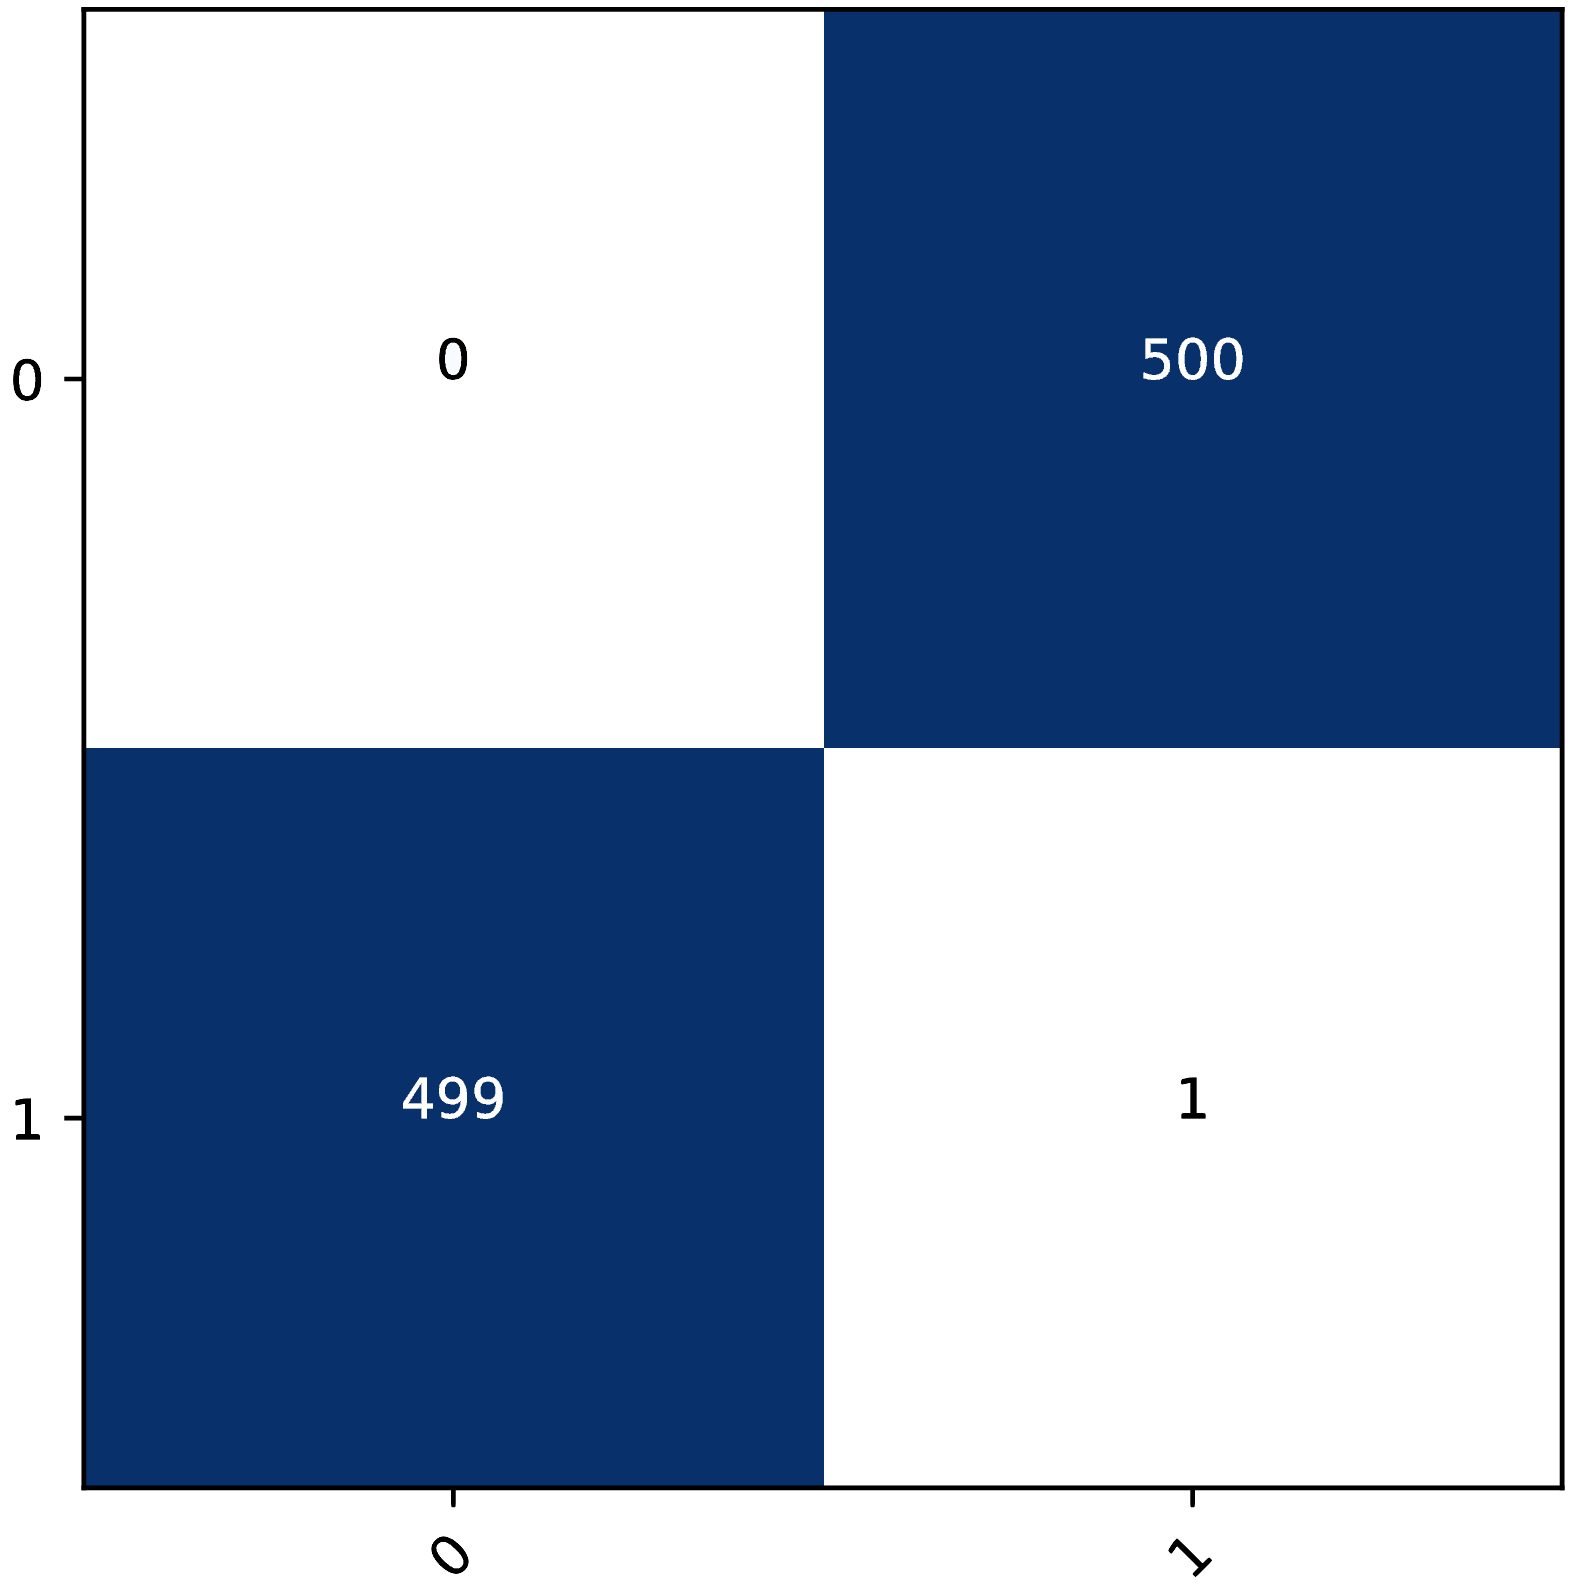
\includegraphics[height=.49\textheight, width=.99\textwidth, keepaspectratio]{moons_confusion_matrix.png}
    \end{minipage}
    \begin{minipage}{.49\textwidth}
        \centering
        \setlength\figureheight{.65\textheight}
        \setlength\figurewidth{1.2\textwidth}
        % This file was created by matplotlib2tikz v0.6.11.
\begin{tikzpicture}

\definecolor{color1}{rgb}{1,0.498039215686275,0.0549019607843137}
\definecolor{color0}{rgb}{0.12156862745098,0.466666666666667,0.705882352941177}
\pgfplotsset{ticks=none}
\begin{axis}[
xmin=-0.0501915524160684, xmax=1.05034307943784,
ymin=-0.0504604147630757, ymax=1.05025716937451,
width=\figurewidth,
height=\figureheight,
tick pos=left
]
\addplot [only marks, mark size=0.5pt, draw=color0, fill=color0, colormap/viridis]
table{%
x                      y
+7.152404189109802e-01 +2.847596406936646e-01
+7.606157064437866e-01 +2.393838316202164e-01
+8.148496150970459e-01 +1.851509511470795e-01
+7.158541679382324e-01 +2.841453850269318e-01
+8.653024435043335e-01 +1.346981823444366e-01
+7.574226260185242e-01 +2.425783723592758e-01
+9.409937262535095e-01 +5.900704488158226e-02
+9.958959817886353e-01 +4.102698527276516e-03
+8.262704610824585e-01 +1.737301796674728e-01
+6.726458072662354e-01 +3.273539841175079e-01
+6.164466738700867e-01 +3.835538029670715e-01
+9.157466292381287e-01 +8.425340056419373e-02
+9.035187363624573e-01 +9.648122638463974e-02
+8.726958632469177e-01 +1.273043155670166e-01
+8.740212917327881e-01 +1.259784847497940e-01
+6.111299991607666e-01 +3.888698518276215e-01
+9.363706707954407e-01 +6.363009661436081e-02
+1.000000000000000e+00 +1.220092061236799e-12
+7.344734668731689e-01 +2.655271589756012e-01
+6.766127943992615e-01 +3.233871757984161e-01
+7.319514751434326e-01 +2.680491209030151e-01
+9.904097914695740e-01 +9.590390138328075e-03
+8.360748887062073e-01 +1.639244705438614e-01
+9.296396374702454e-01 +7.036076486110687e-02
+7.795404195785522e-01 +2.204602360725403e-01
+8.022637367248535e-01 +1.977361738681793e-01
+9.999999403953552e-01 +1.498539887734296e-07
+7.575886249542236e-01 +2.424111515283585e-01
+7.986763119697571e-01 +2.013227492570877e-01
+8.806146979331970e-01 +1.193857863545418e-01
+7.800034284591675e-01 +2.199967503547668e-01
+8.281888365745544e-01 +1.718108206987381e-01
+8.140648007392883e-01 +1.859340816736221e-01
+7.300110459327698e-01 +2.699888944625854e-01
+8.898696303367615e-01 +1.101303994655609e-01
+9.779987335205078e-01 +2.200092375278473e-02
+7.978814840316772e-01 +2.021192163228989e-01
+6.755483150482178e-01 +3.244514763355255e-01
+8.987584710121155e-01 +1.012410148978233e-01
+6.791104078292847e-01 +3.208903074264526e-01
+9.149476885795593e-01 +8.505190163850784e-02
+9.427923560142517e-01 +5.720840394496918e-02
+8.960902690887451e-01 +1.039094179868698e-01
+9.161987900733948e-01 +8.380089700222015e-02
+9.135963916778564e-01 +8.640436083078384e-02
+8.746338486671448e-01 +1.253661364316940e-01
+6.741942763328552e-01 +3.258057832717896e-01
+6.961947083473206e-01 +3.038047850131989e-01
+7.212879061698914e-01 +2.787117660045624e-01
+7.671920657157898e-01 +2.328076958656311e-01
+7.220638990402222e-01 +2.779364287853241e-01
+7.307890057563782e-01 +2.692112624645233e-01
+8.512489795684814e-01 +1.487519592046738e-01
+8.741633892059326e-01 +1.258363574743271e-01
+5.565149784088135e-01 +4.434849023818970e-01
+8.291471600532532e-01 +1.708533614873886e-01
+8.903276324272156e-01 +1.096716821193695e-01
+9.576644897460938e-01 +4.233551397919655e-02
+9.045484662055969e-01 +9.545227885246277e-02
+6.593064069747925e-01 +3.406930565834045e-01
+7.369663119316101e-01 +2.630334794521332e-01
+9.210027456283569e-01 +7.899772375822067e-02
+8.889285922050476e-01 +1.110725104808807e-01
+6.842915415763855e-01 +3.157081902027130e-01
+8.318205475807190e-01 +1.681785583496094e-01
+1.000000000000000e+00 +1.392275075610960e-12
+9.573975205421448e-01 +4.260210692882538e-02
+9.151609539985657e-01 +8.483945578336716e-02
+9.096148014068604e-01 +9.038449078798294e-02
+8.940069079399109e-01 +1.059929728507996e-01
+6.951869726181030e-01 +3.048129975795746e-01
+7.283145785331726e-01 +2.716851532459259e-01
+9.493154287338257e-01 +5.068545415997505e-02
+7.359388470649719e-01 +2.640614211559296e-01
+8.274487257003784e-01 +1.725510209798813e-01
+6.546982526779175e-01 +3.453011810779572e-01
+8.066740632057190e-01 +1.933256685733795e-01
+6.212386488914490e-01 +3.787613213062286e-01
+9.765015244483948e-01 +2.349827066063881e-02
+9.346238970756531e-01 +6.537576764822006e-02
+8.299307823181152e-01 +1.700694710016251e-01
+8.830435276031494e-01 +1.169564500451088e-01
+8.695138692855835e-01 +1.304867267608643e-01
+7.739478945732117e-01 +2.260531932115555e-01
+7.308037281036377e-01 +2.691969275474548e-01
+6.536180973052979e-01 +3.463816940784454e-01
+6.876187324523926e-01 +3.123812675476074e-01
+7.686722278594971e-01 +2.313270717859268e-01
+7.760055065155029e-01 +2.239951938390732e-01
+7.123415470123291e-01 +2.876582741737366e-01
+7.094947099685669e-01 +2.905062437057495e-01
+6.492203474044800e-01 +3.507790863513947e-01
+6.447331905364990e-01 +3.552669882774353e-01
+7.988664507865906e-01 +2.011331170797348e-01
+9.149984121322632e-01 +8.500231057405472e-02
+8.091043233871460e-01 +1.908962279558182e-01
+8.855440616607666e-01 +1.144552975893021e-01
+9.831137657165527e-01 +1.688673906028271e-02
+6.966661810874939e-01 +3.033337295055389e-01
+8.854134082794189e-01 +1.145877912640572e-01
+5.236713290214539e-01 +4.763285815715790e-01
+7.515150308609009e-01 +2.484854161739349e-01
+9.765858650207520e-01 +2.341344580054283e-02
+7.022635936737061e-01 +2.977356314659119e-01
+7.836785316467285e-01 +2.163217961788177e-01
+8.450219035148621e-01 +1.549780368804932e-01
+8.588235378265381e-01 +1.411762386560440e-01
+7.783385515213013e-01 +2.216612994670868e-01
+5.907747745513916e-01 +4.092250764369965e-01
+8.052742481231689e-01 +1.947267502546310e-01
+9.058830738067627e-01 +9.411773830652237e-02
+9.194483160972595e-01 +8.055221289396286e-02
+8.944167494773865e-01 +1.055831983685493e-01
+8.539650440216064e-01 +1.460360884666443e-01
+6.524116396903992e-01 +3.475889265537262e-01
+8.586250543594360e-01 +1.413754820823669e-01
+7.308992743492126e-01 +2.691002190113068e-01
+9.435827136039734e-01 +5.641685798764229e-02
+9.198358058929443e-01 +8.016452938318253e-02
+6.315308213233948e-01 +3.684692084789276e-01
+8.405838608741760e-01 +1.594161391258240e-01
+9.720693826675415e-01 +2.792947553098202e-02
+8.322983384132385e-01 +1.677010357379913e-01
+6.292078495025635e-01 +3.707920312881470e-01
+9.699407815933228e-01 +3.005820512771606e-02
+5.714179873466492e-01 +4.285823106765747e-01
+8.448055386543274e-01 +1.551942378282547e-01
+9.560628533363342e-01 +4.393656179308891e-02
+8.946025967597961e-01 +1.053965464234352e-01
+7.788034677505493e-01 +2.211964428424835e-01
+7.107516527175903e-01 +2.892479300498962e-01
+5.768653750419617e-01 +4.231349527835846e-01
+7.520471811294556e-01 +2.479532808065414e-01
+8.601129055023193e-01 +1.398871243000031e-01
+9.469202160835266e-01 +5.308021977543831e-02
+6.395959258079529e-01 +3.604033589363098e-01
+7.306015491485596e-01 +2.693983018398285e-01
+7.297317981719971e-01 +2.702680230140686e-01
+8.409957289695740e-01 +1.590044349431992e-01
+8.540393710136414e-01 +1.459610611200333e-01
+6.833868622779846e-01 +3.166140615940094e-01
+8.537284731864929e-01 +1.462726444005966e-01
+9.413908123970032e-01 +5.860995873808861e-02
+8.556463718414307e-01 +1.443536728620529e-01
+6.656949520111084e-01 +3.343051671981812e-01
+9.322559833526611e-01 +6.774473935365677e-02
+9.483342766761780e-01 +5.166486650705338e-02
+5.587920546531677e-01 +4.412079751491547e-01
+8.514382243156433e-01 +1.485615372657776e-01
+7.898866534233093e-01 +2.101129740476608e-01
+9.820861220359802e-01 +1.791393570601940e-02
+9.438375234603882e-01 +5.616347491741180e-02
+7.779000997543335e-01 +2.221005558967590e-01
+9.503610730171204e-01 +4.963968694210052e-02
+9.606239795684814e-01 +3.937721624970436e-02
+5.909769535064697e-01 +4.090229868888855e-01
+6.423713564872742e-01 +3.576291799545288e-01
+9.048740267753601e-01 +9.512680023908615e-02
+8.500816822052002e-01 +1.499194949865341e-01
+9.451727271080017e-01 +5.482772737741470e-02
+9.319757223129272e-01 +6.802511960268021e-02
+8.305656909942627e-01 +1.694352775812149e-01
+7.185210585594177e-01 +2.814790010452271e-01
+7.658741474151611e-01 +2.341256737709045e-01
+8.854524493217468e-01 +1.145470812916756e-01
+6.703643202781677e-01 +3.296356499195099e-01
+7.086758613586426e-01 +2.913244962692261e-01
+7.182694077491760e-01 +2.817306220531464e-01
+8.852788805961609e-01 +1.147212311625481e-01
+6.992270946502686e-01 +3.007721006870270e-01
+5.364493727684021e-01 +4.635506570339203e-01
+9.314555525779724e-01 +6.854473799467087e-02
+6.006281375885010e-01 +3.993717133998871e-01
+9.246599078178406e-01 +7.533966749906540e-02
+9.311448931694031e-01 +6.885436177253723e-02
+7.966226339340210e-01 +2.033781111240387e-01
+7.619812488555908e-01 +2.380181699991226e-01
+8.632964491844177e-01 +1.367035061120987e-01
+8.298465013504028e-01 +1.701537072658539e-01
+8.447648882865906e-01 +1.552345752716064e-01
+6.362111568450928e-01 +3.637890219688416e-01
+9.430059194564819e-01 +5.699534714221954e-02
+7.139279842376709e-01 +2.860722839832306e-01
+9.089048504829407e-01 +9.109591692686081e-02
+9.912109375000000e-01 +8.789076469838619e-03
+6.753912568092346e-01 +3.246097564697266e-01
+9.239171743392944e-01 +7.608354836702347e-02
+8.917699456214905e-01 +1.082295477390289e-01
+9.041673541069031e-01 +9.583217650651932e-02
+8.224914669990540e-01 +1.775092929601669e-01
+6.744240522384644e-01 +3.255750238895416e-01
+8.425910472869873e-01 +1.574078202247620e-01
+7.819008827209473e-01 +2.180995792150497e-01
+7.676492333412170e-01 +2.323511689901352e-01
+9.526144266128540e-01 +4.738458618521690e-02
+7.393755316734314e-01 +2.606239616870880e-01
+9.253005385398865e-01 +7.469952851533890e-02
+7.146759629249573e-01 +2.853239774703979e-01
+5.723999738693237e-01 +4.275997281074524e-01
+8.183822035789490e-01 +1.816177964210510e-01
+8.776168227195740e-01 +1.223831400275230e-01
+5.998794436454773e-01 +4.001209139823914e-01
+9.406073093414307e-01 +5.939229950308800e-02
+7.753167152404785e-01 +2.246837168931961e-01
+9.314855933189392e-01 +6.851485371589661e-02
+7.894006967544556e-01 +2.105992287397385e-01
+9.297632575035095e-01 +7.023750990629196e-02
+6.595500111579895e-01 +3.404489457607269e-01
+9.683221578598022e-01 +3.167866170406342e-02
+8.165891170501709e-01 +1.834114640951157e-01
+6.631548404693604e-01 +3.368450403213501e-01
+8.215636610984802e-01 +1.784362941980362e-01
+7.269965410232544e-01 +2.730043828487396e-01
+9.142690300941467e-01 +8.573013544082642e-02
+9.543989300727844e-01 +4.560183361172676e-02
+9.931112527847290e-01 +6.887852679938078e-03
+8.101503252983093e-01 +1.898491978645325e-01
+7.884362936019897e-01 +2.115644663572311e-01
+8.730801343917847e-01 +1.269190907478333e-01
+7.503158450126648e-01 +2.496839761734009e-01
+9.975991249084473e-01 +2.400037599727511e-03
+8.972395062446594e-01 +1.027609258890152e-01
+8.582785129547119e-01 +1.417216658592224e-01
+8.936207294464111e-01 +1.063795387744904e-01
+9.675345420837402e-01 +3.246623277664185e-02
+7.489572167396545e-01 +2.510432898998260e-01
+7.812429666519165e-01 +2.187562882900238e-01
+7.588220238685608e-01 +2.411783635616302e-01
+6.795880794525146e-01 +3.204121291637421e-01
+7.925896644592285e-01 +2.074106335639954e-01
+6.625249385833740e-01 +3.374749422073364e-01
+6.643190979957581e-01 +3.356801867485046e-01
+7.354886531829834e-01 +2.645115554332733e-01
+8.028411269187927e-01 +1.971588283777237e-01
+8.369625806808472e-01 +1.630370765924454e-01
+7.014159560203552e-01 +2.985840737819672e-01
+9.234898090362549e-01 +7.651100307703018e-02
+8.022888898849487e-01 +1.977119296789169e-01
+8.477935791015625e-01 +1.522064357995987e-01
+9.134595990180969e-01 +8.654106408357620e-02
+7.612121701240540e-01 +2.387879937887192e-01
+8.113738298416138e-01 +1.886253952980042e-01
+9.891227483749390e-01 +1.087640412151814e-02
+7.897489070892334e-01 +2.102515846490860e-01
+9.354246258735657e-01 +6.457600742578506e-02
+8.727958202362061e-01 +1.272030025720596e-01
+9.081243276596069e-01 +9.187603741884232e-02
+1.000000000000000e+00 +5.844777244655430e-13
+8.625337481498718e-01 +1.374657601118088e-01
+7.379639148712158e-01 +2.620359361171722e-01
+9.698694348335266e-01 +3.013117983937263e-02
+9.806193709373474e-01 +1.938113756477833e-02
+7.465134263038635e-01 +2.534866333007812e-01
+7.700645327568054e-01 +2.299365550279617e-01
+8.777624368667603e-01 +1.222369000315666e-01
+6.618654727935791e-01 +3.381344079971313e-01
+7.681732773780823e-01 +2.318266332149506e-01
+8.032457232475281e-01 +1.967538595199585e-01
+8.016481995582581e-01 +1.983516663312912e-01
+9.283244609832764e-01 +7.167447358369827e-02
+7.077567577362061e-01 +2.922425568103790e-01
+8.009940981864929e-01 +1.990070343017578e-01
+9.775995016098022e-01 +2.240156941115856e-02
+9.464283585548401e-01 +5.357155948877335e-02
+9.148731827735901e-01 +8.512684702873230e-02
+7.402006387710571e-01 +2.597998380661011e-01
+8.283989429473877e-01 +1.716020554304123e-01
+8.420336246490479e-01 +1.579658389091492e-01
+8.603492975234985e-01 +1.396510899066925e-01
+8.804780840873718e-01 +1.195214390754700e-01
+7.996644377708435e-01 +2.003358453512192e-01
+7.630436420440674e-01 +2.369561642408371e-01
+6.855850815773010e-01 +3.144149482250214e-01
+7.936196327209473e-01 +2.063806951045990e-01
+9.375007152557373e-01 +6.249821558594704e-02
+7.637969255447388e-01 +2.362028509378433e-01
+6.128731369972229e-01 +3.871268033981323e-01
+8.761802911758423e-01 +1.238200739026070e-01
+7.536247372627258e-01 +2.463742792606354e-01
+8.969962596893311e-01 +1.030026227235794e-01
+8.550719618797302e-01 +1.449282318353653e-01
+9.204356670379639e-01 +7.956350594758987e-02
+8.295968770980835e-01 +1.704035550355911e-01
+6.589993834495544e-01 +3.410012722015381e-01
+8.710854053497314e-01 +1.289158016443253e-01
+8.584159612655640e-01 +1.415836960077286e-01
+8.643237948417664e-01 +1.356766521930695e-01
+9.099126458168030e-01 +9.008662402629852e-02
+9.368386864662170e-01 +6.316088885068893e-02
+7.917550802230835e-01 +2.082456350326538e-01
+8.605650067329407e-01 +1.394355446100235e-01
+6.651690006256104e-01 +3.348308205604553e-01
+8.938543200492859e-01 +1.061455085873604e-01
+8.146643638610840e-01 +1.853358298540115e-01
+6.374320387840271e-01 +3.625682592391968e-01
+6.953687071800232e-01 +3.046317994594574e-01
+9.951547384262085e-01 +4.846512805670500e-03
+7.831878066062927e-01 +2.168123126029968e-01
+8.478192687034607e-01 +1.521799713373184e-01
+7.038489580154419e-01 +2.961520850658417e-01
+8.070116639137268e-01 +1.929885745048523e-01
+9.692375659942627e-01 +3.076360933482647e-02
+7.694165706634521e-01 +2.305838465690613e-01
+9.998857378959656e-01 +1.138766238000244e-04
+8.245673179626465e-01 +1.754330247640610e-01
+8.154172301292419e-01 +1.845828443765640e-01
+7.729795575141907e-01 +2.270207852125168e-01
+8.038964867591858e-01 +1.961033195257187e-01
+7.433089613914490e-01 +2.566911280155182e-01
+6.994323134422302e-01 +3.005677461624146e-01
+8.058241009712219e-01 +1.941763162612915e-01
+7.410042285919189e-01 +2.589963972568512e-01
+7.892889976501465e-01 +2.107110768556595e-01
+7.147701978683472e-01 +2.852302193641663e-01
+9.088848233222961e-01 +9.111445397138596e-02
+8.403118848800659e-01 +1.596879810094833e-01
+8.353173136711121e-01 +1.646824479103088e-01
+9.709644317626953e-01 +2.903509326279163e-02
+9.452667832374573e-01 +5.473278835415840e-02
+7.452927231788635e-01 +2.547073066234589e-01
+6.129180788993835e-01 +3.870823383331299e-01
+6.489097476005554e-01 +3.510908186435699e-01
+9.911245703697205e-01 +8.876439183950424e-03
+7.234573960304260e-01 +2.765426337718964e-01
+9.141309857368469e-01 +8.586975932121277e-02
+8.805645704269409e-01 +1.194346547126770e-01
+6.093061566352844e-01 +3.906939625740051e-01
+7.675399780273438e-01 +2.324600219726562e-01
+8.557761907577515e-01 +1.442234218120575e-01
+7.417577505111694e-01 +2.582418024539948e-01
+7.840322256088257e-01 +2.159677147865295e-01
+8.913492560386658e-01 +1.086515039205551e-01
+7.425229549407959e-01 +2.574773728847504e-01
+1.000000000000000e+00 +2.354050114561357e-13
+6.911781430244446e-01 +3.088211119174957e-01
+6.882238984107971e-01 +3.117770850658417e-01
+7.697073221206665e-01 +2.302919924259186e-01
+6.825291514396667e-01 +3.174706697463989e-01
+5.648832917213440e-01 +4.351169466972351e-01
+7.641898989677429e-01 +2.358110994100571e-01
+8.245923519134521e-01 +1.754082739353180e-01
+6.943407654762268e-01 +3.056588470935822e-01
+7.572834491729736e-01 +2.427164465188980e-01
+7.839691042900085e-01 +2.160302549600601e-01
+7.863542437553406e-01 +2.136453986167908e-01
+8.143918514251709e-01 +1.856086850166321e-01
+9.207382798194885e-01 +7.926131039857864e-02
+9.611822366714478e-01 +3.881650045514107e-02
+8.141553997993469e-01 +1.858450770378113e-01
+9.387455582618713e-01 +6.125434860587120e-02
+7.114598155021667e-01 +2.885398864746094e-01
+9.174249172210693e-01 +8.257579058408737e-02
+8.645269870758057e-01 +1.354731917381287e-01
+7.276847958564758e-01 +2.723144888877869e-01
+7.652511000633240e-01 +2.347489744424820e-01
+6.516721248626709e-01 +3.483279943466187e-01
+8.132637143135071e-01 +1.867353469133377e-01
+7.638733386993408e-01 +2.361260950565338e-01
+8.663632869720459e-01 +1.336374133825302e-01
+9.562551379203796e-01 +4.374435916543007e-02
+7.883957028388977e-01 +2.116050124168396e-01
+8.188675642013550e-01 +1.811330616474152e-01
+8.429384827613831e-01 +1.570625156164169e-01
+6.039779782295227e-01 +3.960216641426086e-01
+7.167079448699951e-01 +2.832926511764526e-01
+8.016387224197388e-01 +1.983604580163956e-01
+6.570740342140198e-01 +3.429259061813354e-01
+7.222474813461304e-01 +2.777524292469025e-01
+8.208625316619873e-01 +1.791364848613739e-01
+8.287893533706665e-01 +1.712100356817245e-01
+9.015630483627319e-01 +9.843738377094269e-02
+7.471662759780884e-01 +2.528341710567474e-01
+7.008057236671448e-01 +2.991942465305328e-01
+9.014281630516052e-01 +9.857209026813507e-02
+7.472907304763794e-01 +2.527103424072266e-01
+7.123715877532959e-01 +2.876286804676056e-01
+9.665583968162537e-01 +3.344201669096947e-02
+6.484795212745667e-01 +3.515205085277557e-01
+8.142441511154175e-01 +1.857565045356750e-01
+8.810813426971436e-01 +1.189175397157669e-01
+9.232712388038635e-01 +7.672847062349319e-02
+8.458300828933716e-01 +1.541702300310135e-01
+8.501356244087219e-01 +1.498648971319199e-01
+7.249476909637451e-01 +2.750526070594788e-01
+9.610284566879272e-01 +3.897279128432274e-02
+7.462188601493835e-01 +2.537816762924194e-01
+8.265862464904785e-01 +1.734133660793304e-01
+8.552038669586182e-01 +1.447961628437042e-01
+8.622333407402039e-01 +1.377668529748917e-01
+7.297776937484741e-01 +2.702221572399139e-01
+7.462280392646790e-01 +2.537721395492554e-01
+6.250618100166321e-01 +3.749376237392426e-01
+9.027277231216431e-01 +9.727160632610321e-02
+8.787689805030823e-01 +1.212310045957565e-01
+7.291228771209717e-01 +2.708773910999298e-01
+8.085807561874390e-01 +1.914194226264954e-01
+9.565982818603516e-01 +4.340141639113426e-02
+8.561652898788452e-01 +1.438343226909637e-01
+9.883781671524048e-01 +1.162244100123644e-02
+9.428864121437073e-01 +5.711321532726288e-02
+8.498076796531677e-01 +1.501925140619278e-01
+9.587682485580444e-01 +4.123300686478615e-02
+9.987794756889343e-01 +1.219920697622001e-03
+8.176950216293335e-01 +1.823054701089859e-01
+7.377785444259644e-01 +2.622204124927521e-01
+9.867933392524719e-01 +1.320731546729803e-02
+9.322822093963623e-01 +6.771671026945114e-02
+6.657439470291138e-01 +3.342565894126892e-01
+9.927496314048767e-01 +7.251481991261244e-03
+7.714464068412781e-01 +2.285532504320145e-01
+7.789765000343323e-01 +2.210235446691513e-01
+8.809134960174561e-01 +1.190856173634529e-01
+9.556374549865723e-01 +4.436179623007774e-02
+7.368189096450806e-01 +2.631812393665314e-01
+6.800234317779541e-01 +3.199763596057892e-01
+5.821561217308044e-01 +4.178442358970642e-01
+9.057867527008057e-01 +9.421256184577942e-02
+7.531540393829346e-01 +2.468453943729401e-01
+7.081028223037720e-01 +2.918968498706818e-01
+8.074423074722290e-01 +1.925571262836456e-01
+6.925249695777893e-01 +3.074746429920197e-01
+9.129770398139954e-01 +8.702288568019867e-02
+7.668917179107666e-01 +2.331078648567200e-01
+9.731523394584656e-01 +2.684713155031204e-02
+6.944705843925476e-01 +3.055286705493927e-01
+9.119089245796204e-01 +8.809130638837814e-02
+6.426591277122498e-01 +3.573401570320129e-01
+8.829950094223022e-01 +1.170056760311127e-01
+6.935722827911377e-01 +3.064284324645996e-01
+9.582449197769165e-01 +4.175424575805664e-02
+8.778151869773865e-01 +1.221849918365479e-01
+6.552963852882385e-01 +3.447035551071167e-01
+9.394301772117615e-01 +6.057008355855942e-02
+6.705324649810791e-01 +3.294663727283478e-01
+7.741698622703552e-01 +2.258300930261612e-01
+8.627777695655823e-01 +1.372220367193222e-01
+9.968724250793457e-01 +3.127077128738165e-03
+8.977100849151611e-01 +1.022901609539986e-01
+8.370435237884521e-01 +1.629572063684464e-01
+8.662721514701843e-01 +1.337272971868515e-01
+9.195868968963623e-01 +8.041200786828995e-02
+5.811195373535156e-01 +4.188804924488068e-01
+6.749352216720581e-01 +3.250638246536255e-01
+8.813933730125427e-01 +1.186068132519722e-01
+6.958438754081726e-01 +3.041554689407349e-01
+7.291343212127686e-01 +2.708650231361389e-01
+8.826975226402283e-01 +1.173029690980911e-01
+8.360069394111633e-01 +1.639919430017471e-01
+7.373173236846924e-01 +2.626824080944061e-01
+9.600518941879272e-01 +3.994912281632423e-02
+7.451294064521790e-01 +2.548708915710449e-01
+8.775398731231689e-01 +1.224612519145012e-01
+8.884042501449585e-01 +1.115964353084564e-01
+7.124830484390259e-01 +2.875171303749084e-01
+8.225257992744446e-01 +1.774731278419495e-01
+7.993112206459045e-01 +2.006887048482895e-01
+6.195449233055115e-01 +3.804550468921661e-01
+6.967841386795044e-01 +3.032168149948120e-01
+9.654109477996826e-01 +3.458786383271217e-02
+8.445516824722290e-01 +1.554477661848068e-01
+9.069082736968994e-01 +9.309134632349014e-02
+8.501227498054504e-01 +1.498772948980331e-01
+7.111161947250366e-01 +2.888837158679962e-01
+8.150405287742615e-01 +1.849594265222549e-01
+7.184098958969116e-01 +2.815899252891541e-01
+7.820007205009460e-01 +2.179986834526062e-01
+8.917644023895264e-01 +1.082352697849274e-01
+6.108254790306091e-01 +3.891741633415222e-01
+7.576438784599304e-01 +2.423567771911621e-01
+6.930035948753357e-01 +3.069968223571777e-01
+7.248813509941101e-01 +2.751182913780212e-01
+7.777031064033508e-01 +2.222958952188492e-01
+8.681790828704834e-01 +1.318216174840927e-01
+6.720583438873291e-01 +3.279404938220978e-01
+7.378234267234802e-01 +2.621766328811646e-01
+6.974332332611084e-01 +3.025670349597931e-01
+8.591989874839783e-01 +1.408014446496964e-01
+8.298265933990479e-01 +1.701726317405701e-01
+8.401288390159607e-01 +1.598708629608154e-01
+7.198256850242615e-01 +2.801742851734161e-01
+7.721326947212219e-01 +2.278676480054855e-01
+5.883982181549072e-01 +4.116016626358032e-01
+7.507814168930054e-01 +2.492180019617081e-01
+8.552245497703552e-01 +1.447754055261612e-01
+9.976344108581543e-01 +2.366259926930070e-03
+8.013581037521362e-01 +1.986427158117294e-01
+9.629721641540527e-01 +3.702853620052338e-02
+8.843661546707153e-01 +1.156345903873444e-01
+8.689172267913818e-01 +1.310832053422928e-01
+9.232102036476135e-01 +7.678938657045364e-02
+8.117452859878540e-01 +1.882540136575699e-01
+6.638447046279907e-01 +3.361553251743317e-01
+9.528024792671204e-01 +4.719800874590874e-02
+8.855541944503784e-01 +1.144450455904007e-01
+9.941254258155823e-01 +5.874182097613811e-03
+8.502655625343323e-01 +1.497344821691513e-01
+7.355887889862061e-01 +2.644105553627014e-01
+6.783828735351562e-01 +3.216171264648438e-01
+9.422988295555115e-01 +5.770142376422882e-02
};
\addplot [only marks, mark size=0.5pt, draw=color1, fill=color1, colormap/viridis]
table{%
x                      y
+2.544288337230682e-01 +7.455717325210571e-01
+2.563878297805786e-01 +7.436116933822632e-01
+3.339706063270569e-01 +6.660301089286804e-01
+3.291154205799103e-01 +6.708838939666748e-01
+2.328986674547195e-01 +7.671020030975342e-01
+3.201881349086761e-01 +6.798124909400940e-01
+5.320103093981743e-02 +9.467996954917908e-01
+7.808157801628113e-02 +9.219186902046204e-01
+4.069714620709419e-02 +9.593029022216797e-01
+1.200221329927444e-01 +8.799771070480347e-01
+4.732818305492401e-01 +5.267181992530823e-01
+2.462228387594223e-01 +7.537767887115479e-01
+3.128810226917267e-01 +6.871187686920166e-01
+1.324463486671448e-01 +8.675536513328552e-01
+2.018564343452454e-01 +7.981438636779785e-01
+2.659611403942108e-01 +7.340391278266907e-01
+6.154919043183327e-02 +9.384512305259705e-01
+3.053403459489346e-02 +9.694666266441345e-01
+1.244726851582527e-01 +8.755266666412354e-01
+7.314790040254593e-02 +9.268515110015869e-01
+3.365139067173004e-01 +6.634861826896667e-01
+2.897882275283337e-02 +9.710216522216797e-01
+1.511776447296143e-01 +8.488229513168335e-01
+1.124966368079185e-01 +8.875039815902710e-01
+1.297482848167419e-01 +8.702522516250610e-01
+1.649124771356583e-01 +8.350878953933716e-01
+9.455642849206924e-02 +9.054433703422546e-01
+2.255558222532272e-02 +9.774451255798340e-01
+1.567203551530838e-01 +8.432792425155640e-01
+2.838727235794067e-01 +7.161263227462769e-01
+3.655700385570526e-01 +6.344299912452698e-01
+1.698456406593323e-01 +8.301543593406677e-01
+2.732385694980621e-01 +7.267611026763916e-01
+2.927132844924927e-01 +7.072863578796387e-01
+2.818545997142792e-01 +7.181464433670044e-01
+3.043256103992462e-01 +6.956743597984314e-01
+2.089271135628223e-02 +9.791082739830017e-01
+2.042180597782135e-01 +7.957816123962402e-01
+2.456264495849609e-01 +7.543740868568420e-01
+3.123129606246948e-01 +6.876872181892395e-01
+2.630852133367334e-12 +1.000000000000000e+00
+3.952292501926422e-01 +6.047707200050354e-01
+2.608242332935333e-01 +7.391747236251831e-01
+8.214231580495834e-02 +9.178569316864014e-01
+1.612901538610458e-01 +8.387097120285034e-01
+3.675037026405334e-01 +6.324965953826904e-01
+4.450675100088120e-02 +9.554924964904785e-01
+3.061546385288239e-01 +6.938448548316956e-01
+4.863114282488823e-02 +9.513697028160095e-01
+2.642263770103455e-01 +7.357738614082336e-01
+1.001214757561684e-01 +8.998792767524719e-01
+9.380109608173370e-02 +9.061986804008484e-01
+2.227292805910110e-01 +7.772704362869263e-01
+1.583662182092667e-01 +8.416339159011841e-01
+2.358301728963852e-01 +7.641702294349670e-01
+2.918720543384552e-01 +7.081272602081299e-01
+2.180163562297821e-01 +7.819826602935791e-01
+1.136160790920258e-01 +8.863832950592041e-01
+3.816528245806694e-02 +9.618353843688965e-01
+2.737847566604614e-01 +7.262148261070251e-01
+2.764092683792114e-01 +7.235903143882751e-01
+2.608890831470490e-01 +7.391103506088257e-01
+3.892174959182739e-01 +6.107825636863708e-01
+1.687306165695190e-01 +8.312689065933228e-01
+2.899050414562225e-01 +7.100950479507446e-01
+2.397893369197845e-01 +7.602107524871826e-01
+6.384623050689697e-02 +9.361546039581299e-01
+2.610188722610474e-01 +7.389806509017944e-01
+3.340606987476349e-01 +6.659392714500427e-01
+1.527900546789169e-01 +8.472109436988831e-01
+9.929809719324112e-02 +9.007027149200439e-01
+8.034607768058777e-02 +9.196546673774719e-01
+4.222732409834862e-02 +9.577718377113342e-01
+1.136818826198578e-01 +8.863171339035034e-01
+1.120004430413246e-01 +8.880002498626709e-01
+2.514913976192474e-01 +7.485090494155884e-01
+1.829422414302826e-01 +8.170575499534607e-01
+2.718472182750702e-01 +7.281525135040283e-01
+2.427673786878586e-01 +7.572326064109802e-01
+2.151055932044983e-01 +7.848943471908569e-01
+1.787016093730927e-01 +8.212974071502686e-01
+1.367833912372589e-01 +8.632174134254456e-01
+2.919296622276306e-01 +7.080695629119873e-01
+2.559274435043335e-01 +7.440721988677979e-01
+1.304757148027420e-01 +8.695242404937744e-01
+1.906694024801254e-01 +8.093308806419373e-01
+1.835028678178787e-01 +8.164976239204407e-01
+3.363918066024780e-01 +6.636082530021667e-01
+6.699896603822708e-02 +9.330006241798401e-01
+2.477709203958511e-01 +7.522280216217041e-01
+1.685841381549835e-01 +8.314156532287598e-01
+9.371469169855118e-02 +9.062860012054443e-01
+8.177516609430313e-02 +9.182256460189819e-01
+3.034991025924683e-01 +6.965018510818481e-01
+1.940763443708420e-01 +8.059235215187073e-01
+1.072515025734901e-01 +8.927481770515442e-01
+8.017433434724808e-02 +9.198251962661743e-01
+1.351998299360275e-01 +8.647995591163635e-01
+1.544168144464493e-01 +8.455832600593567e-01
+1.464169174432755e-01 +8.535836935043335e-01
+8.196579664945602e-02 +9.180349111557007e-01
+1.925264745950699e-01 +8.074728250503540e-01
+6.261392682790756e-02 +9.373857378959656e-01
+4.424423445016146e-03 +9.955751299858093e-01
+2.193242609500885e-01 +7.806754112243652e-01
+2.593835890293121e-01 +7.406160831451416e-01
+2.984238862991333e-01 +7.015761733055115e-01
+2.850395143032074e-01 +7.149608135223389e-01
+1.549828331917524e-02 +9.845023155212402e-01
+2.780813872814178e-01 +7.219189405441284e-01
+2.134902328252792e-01 +7.865095734596252e-01
+2.062187343835831e-01 +7.937805056571960e-01
+3.426055908203125e-01 +6.573943495750427e-01
+2.453999519348145e-01 +7.546003460884094e-01
+3.926338851451874e-01 +6.073656082153320e-01
+6.024090200662613e-02 +9.397584795951843e-01
+3.678321465849876e-02 +9.632180929183960e-01
+1.565313190221786e-01 +8.434682488441467e-01
+3.519872426986694e-01 +6.480132937431335e-01
+1.407813876867294e-01 +8.592194914817810e-01
+1.995408982038498e-01 +8.004600405693054e-01
+6.024186499416828e-03 +9.939750432968140e-01
+1.398200988769531e-01 +8.601807951927185e-01
+1.151549592614174e-01 +8.848445415496826e-01
+1.158322393894196e-01 +8.841683268547058e-01
+2.999702394008636e-01 +7.000302672386169e-01
+2.757168114185333e-01 +7.242821455001831e-01
+1.617546230554581e-01 +8.382444977760315e-01
+1.535823345184326e-01 +8.464180231094360e-01
+3.244204223155975e-01 +6.755795478820801e-01
+3.227138221263885e-01 +6.772851347923279e-01
+1.674298346042633e-01 +8.325705528259277e-01
+2.537040412425995e-01 +7.462954521179199e-01
+2.088125348091125e-01 +7.911881208419800e-01
+2.289071530103683e-01 +7.710927724838257e-01
+2.968331575393677e-01 +7.031666040420532e-01
+1.619463413953781e-01 +8.380532264709473e-01
+3.465364873409271e-01 +6.534643769264221e-01
+1.707751303911209e-01 +8.292242288589478e-01
+4.687690436840057e-01 +5.312309265136719e-01
+3.786391913890839e-01 +6.213608384132385e-01
+1.314022839069366e-01 +8.685983419418335e-01
+5.102824047207832e-02 +9.489725232124329e-01
+1.465461105108261e-01 +8.534544110298157e-01
+1.127852723002434e-01 +8.872147202491760e-01
+3.200354874134064e-01 +6.799650788307190e-01
+1.490208953619003e-01 +8.509798645973206e-01
+2.194940149784088e-01 +7.805053591728210e-01
+2.892776131629944e-01 +7.107231616973877e-01
+1.211574003100395e-01 +8.788430094718933e-01
+9.942781180143356e-02 +9.005730152130127e-01
+2.088436856865883e-02 +9.791162610054016e-01
+1.391871124505997e-01 +8.608121275901794e-01
+4.436011291370640e-13 +1.000000000000000e+00
+2.269935607910156e-01 +7.730070352554321e-01
+1.707151383161545e-01 +8.292847275733948e-01
+1.514546722173691e-01 +8.485460877418518e-01
+1.226879954338074e-01 +8.773117661476135e-01
+1.689862012863159e-01 +8.310141563415527e-01
+3.712879419326782e-01 +6.287119388580322e-01
+1.263294965028763e-01 +8.736703395843506e-01
+2.519859969615936e-01 +7.480137348175049e-01
+3.408860787749290e-02 +9.659118056297302e-01
+1.411288082599640e-01 +8.588714003562927e-01
+3.509008288383484e-01 +6.490984559059143e-01
+3.609657585620880e-01 +6.390343308448792e-01
+2.298337370157242e-01 +7.701652646064758e-01
+1.594686061143875e-01 +8.405309915542603e-01
+1.091623529791832e-01 +8.908380866050720e-01
+1.968410164117813e-01 +8.031591773033142e-01
+1.330897957086563e-01 +8.669106364250183e-01
+5.507309734821320e-02 +9.449259042739868e-01
+1.599387973546982e-01 +8.400620818138123e-01
+1.224282458424568e-01 +8.775712847709656e-01
+1.895238906145096e-01 +8.104759454727173e-01
+1.187365278601646e-01 +8.812636733055115e-01
+9.491910785436630e-02 +9.050819873809814e-01
+2.981160208582878e-02 +9.701895117759705e-01
+1.898625493049622e-01 +8.101372718811035e-01
+9.005390107631683e-02 +9.099453091621399e-01
+7.190039753913879e-02 +9.281000494956970e-01
+2.471289783716202e-01 +7.528712749481201e-01
+1.417253166437149e-01 +8.582756519317627e-01
+3.614373803138733e-01 +6.385620236396790e-01
+3.026194572448730e-01 +6.973803043365479e-01
+3.368895053863525e-01 +6.631097197532654e-01
+1.900998950004578e-01 +8.098991513252258e-01
+2.106894105672836e-01 +7.893112301826477e-01
+2.287382483482361e-01 +7.712624073028564e-01
+9.363238513469696e-02 +9.063669443130493e-01
+2.396412342786789e-01 +7.603582739830017e-01
+2.464586496353149e-01 +7.535406351089478e-01
+4.970244467258453e-01 +5.029755234718323e-01
+3.923153504729271e-02 +9.607691168785095e-01
+9.642791748046875e-02 +9.035720825195312e-01
+1.386003345251083e-01 +8.613994717597961e-01
+2.114753872156143e-01 +7.885252237319946e-01
+9.884073585271835e-02 +9.011591076850891e-01
+8.859314024448395e-02 +9.114072918891907e-01
+2.964978516101837e-01 +7.035020589828491e-01
+2.110297232866287e-01 +7.889707088470459e-01
+2.695413231849670e-01 +7.304584383964539e-01
+8.490413427352905e-02 +9.150950908660889e-01
+1.087360680103302e-01 +8.912637829780579e-01
+1.022072583436966e-01 +8.977916836738586e-01
+3.251513540744781e-01 +6.748495697975159e-01
+1.613102108240128e-01 +8.386895060539246e-01
+2.010613977909088e-01 +7.989379763603210e-01
+1.949398219585419e-01 +8.050607442855835e-01
+6.928072869777679e-02 +9.307181835174561e-01
+1.411059200763702e-01 +8.588942885398865e-01
+2.277296185493469e-01 +7.722702622413635e-01
+1.752881109714508e-01 +8.247122764587402e-01
+1.770027577877045e-01 +8.229978680610657e-01
+2.364572137594223e-01 +7.635424137115479e-01
+2.440923303365707e-01 +7.559077739715576e-01
+2.463876968249679e-03 +9.975357651710510e-01
+3.607886135578156e-01 +6.392107009887695e-01
+3.462103605270386e-01 +6.537896990776062e-01
+3.019309937953949e-01 +6.980695128440857e-01
+2.914198637008667e-01 +7.085800766944885e-01
+1.878159940242767e-01 +8.121843934059143e-01
+2.982591986656189e-01 +7.017408013343811e-01
+2.849813103675842e-01 +7.150185108184814e-01
+3.267287909984589e-01 +6.732712388038635e-01
+7.681561261415482e-02 +9.231847524642944e-01
+2.788385748863220e-01 +7.211611270904541e-01
+2.372422367334366e-01 +7.627570629119873e-01
+3.480682671070099e-01 +6.519317030906677e-01
+6.232405081391335e-02 +9.376755356788635e-01
+1.273371577262878e-01 +8.726632595062256e-01
+2.936667203903198e-01 +7.063336372375488e-01
+3.044971525669098e-01 +6.955029964447021e-01
+7.086989283561707e-02 +9.291304945945740e-01
+2.461400181055069e-01 +7.538602352142334e-01
+2.400113642215729e-01 +7.599876523017883e-01
+8.619116991758347e-02 +9.138100147247314e-01
+3.089695274829865e-01 +6.910297274589539e-01
+5.267017707228661e-02 +9.473291039466858e-01
+4.613636434078217e-02 +9.538645148277283e-01
+3.876187205314636e-01 +6.123810410499573e-01
+1.647379249334335e-01 +8.352614045143127e-01
+1.076161563396454e-01 +8.923847079277039e-01
+1.785118877887726e-01 +8.214876055717468e-01
+1.934106796979904e-01 +8.065896034240723e-01
+2.630366086959839e-01 +7.369638681411743e-01
+1.197665333747864e-01 +8.802337050437927e-01
+2.956446409225464e-01 +7.043560147285461e-01
+3.039040565490723e-01 +6.960955262184143e-01
+3.631232380867004e-01 +6.368760466575623e-01
+2.146988511085510e-01 +7.853011488914490e-01
+1.688478291034698e-01 +8.311531543731689e-01
+2.889806032180786e-01 +7.110187411308289e-01
+2.027161270380020e-01 +7.972840666770935e-01
+2.391737401485443e-01 +7.608261704444885e-01
+1.820108853280544e-02 +9.817983508110046e-01
+3.106151521205902e-01 +6.893846988677979e-01
+2.717398405075073e-01 +7.282605767250061e-01
+1.997587233781815e-01 +8.002402782440186e-01
+1.403386443853378e-01 +8.596621155738831e-01
+1.278991848230362e-01 +8.721007704734802e-01
+5.940071493387222e-02 +9.405982494354248e-01
+1.303326636552811e-01 +8.696671128273010e-01
+1.977609246969223e-01 +8.022386431694031e-01
+2.412592470645905e-01 +7.587406635284424e-01
+3.209152519702911e-01 +6.790847182273865e-01
+2.223128825426102e-01 +7.776871323585510e-01
+2.107174843549728e-01 +7.892831563949585e-01
+3.323918879032135e-01 +6.676073670387268e-01
+1.223958209156990e-01 +8.776037693023682e-01
+1.598272919654846e-01 +8.401720523834229e-01
+3.395466208457947e-01 +6.604535579681396e-01
+2.134606614708900e-02 +9.786534309387207e-01
+7.179164886474609e-02 +9.282076358795166e-01
+3.016900829970837e-02 +9.698314666748047e-01
+1.498393863439560e-01 +8.501608967781067e-01
+8.384850621223450e-02 +9.161523580551147e-01
+3.577111661434174e-02 +9.642281532287598e-01
+1.683800369501114e-01 +8.316194415092468e-01
+2.129247784614563e-01 +7.870758175849915e-01
+2.771033942699432e-01 +7.228970527648926e-01
+3.088649809360504e-01 +6.911349296569824e-01
+8.199552446603775e-02 +9.180047512054443e-01
+2.645659744739532e-01 +7.354347705841064e-01
+2.361539453268051e-01 +7.638466358184814e-01
+2.669468224048615e-01 +7.330526113510132e-01
+1.070823743939400e-01 +8.929165601730347e-01
+2.795982062816620e-01 +7.204022407531738e-01
+3.335498869419098e-01 +6.664502620697021e-01
+5.968223884701729e-02 +9.403173327445984e-01
+6.223343685269356e-02 +9.377669692039490e-01
+1.644132584333420e-01 +8.355866074562073e-01
+2.383923977613449e-01 +7.616073489189148e-01
+2.664166688919067e-01 +7.335823178291321e-01
+2.264593243598938e-01 +7.735412716865540e-01
+3.250890597701073e-02 +9.674910902976990e-01
+2.542590796947479e-01 +7.457419633865356e-01
+1.636238694190979e-01 +8.363752961158752e-01
+2.357109636068344e-02 +9.764276146888733e-01
+2.370161563158035e-01 +7.629845142364502e-01
+1.795213818550110e-01 +8.204795718193054e-01
+3.122197389602661e-01 +6.877795457839966e-01
+3.019180595874786e-01 +6.980819106101990e-01
+1.623725295066833e-01 +8.376283049583435e-01
+3.402899503707886e-01 +6.597101092338562e-01
+2.605508863925934e-01 +7.394487857818604e-01
+1.650581508874893e-01 +8.349409699440002e-01
+2.255127876996994e-01 +7.744873762130737e-01
+9.003509581089020e-02 +9.099653363227844e-01
+1.595833152532578e-01 +8.404161334037781e-01
+2.050172388553619e-01 +7.949828505516052e-01
+2.303581386804581e-01 +7.696411609649658e-01
+1.170352399349213e-01 +8.829650282859802e-01
+1.873302608728409e-01 +8.126686215400696e-01
+5.190992355346680e-02 +9.480896592140198e-01
+1.132468506693840e-01 +8.867541551589966e-01
+2.296163141727448e-01 +7.703832983970642e-01
+3.415220230817795e-02 +9.658484458923340e-01
+3.491321206092834e-01 +6.508677601814270e-01
+1.419991850852966e-01 +8.580014705657959e-01
+7.908422723114372e-13 +1.000000000000000e+00
+2.828173935413361e-01 +7.171827554702759e-01
+9.820460528135300e-02 +9.017946720123291e-01
+1.089537441730499e-01 +8.910453319549561e-01
+2.742390036582947e-01 +7.257611751556396e-01
+8.487221598625183e-02 +9.151284694671631e-01
+2.105802744626999e-01 +7.894204854965210e-01
+9.417618811130524e-02 +9.058232903480530e-01
+7.363281399011612e-02 +9.263681173324585e-01
+2.222620993852615e-01 +7.777379751205444e-01
+2.905923128128052e-01 +7.094073295593262e-01
+2.686952650547028e-01 +7.313048839569092e-01
+2.323816418647766e-01 +7.676187157630920e-01
+1.902687102556229e-01 +8.097307682037354e-01
+1.976434290409088e-01 +8.023558855056763e-01
+5.957888439297676e-02 +9.404218196868896e-01
+3.623716831207275e-01 +6.376276612281799e-01
+2.190888524055481e-01 +7.809113860130310e-01
+3.452987372875214e-01 +6.547012329101562e-01
+5.005628243088722e-02 +9.499436020851135e-01
+9.168370068073273e-02 +9.083170294761658e-01
+1.447449326515198e-01 +8.552550673484802e-01
+2.597140967845917e-01 +7.402869462966919e-01
+4.700427129864693e-02 +9.529953598976135e-01
+3.731282353401184e-01 +6.268722414970398e-01
+3.036084473133087e-01 +6.963915228843689e-01
+2.721094787120819e-01 +7.278902530670166e-01
+2.176183760166168e-01 +7.823816537857056e-01
+2.344894558191299e-01 +7.655104994773865e-01
+3.357003675773740e-03 +9.966430068016052e-01
+3.297163918614388e-02 +9.670278429985046e-01
+3.207703828811646e-01 +6.792296767234802e-01
+4.716019332408905e-02 +9.528402686119080e-01
+1.293466240167618e-01 +8.706533908843994e-01
+3.320308029651642e-01 +6.679689884185791e-01
+3.239821195602417e-01 +6.760178208351135e-01
+1.202612593770027e-01 +8.797380924224854e-01
+2.392926216125488e-01 +7.607071399688721e-01
+3.534432649612427e-01 +6.465566158294678e-01
+1.507473140954971e-01 +8.492515087127686e-01
+8.185342699289322e-02 +9.181463122367859e-01
+1.925124973058701e-01 +8.074875473976135e-01
+2.193742543458939e-01 +7.806249856948853e-01
+2.945842742919922e-01 +7.054147124290466e-01
+1.285849213600159e-01 +8.714144229888916e-01
+1.827850937843323e-01 +8.172149062156677e-01
+1.050564199686050e-01 +8.949432969093323e-01
+7.036577165126801e-02 +9.296341538429260e-01
+2.792602181434631e-01 +7.207405567169189e-01
+1.852428317070007e-01 +8.147577047348022e-01
+3.649558722972870e-01 +6.350441575050354e-01
+3.350716456770897e-02 +9.664922356605530e-01
+2.588295936584473e-01 +7.411701083183289e-01
+3.522431254386902e-01 +6.477575898170471e-01
+3.000568747520447e-01 +6.999433040618896e-01
+1.898689270019531e-01 +8.101318478584290e-01
+1.600303053855896e-01 +8.399705290794373e-01
+4.579131677746773e-02 +9.542084336280823e-01
+2.912045717239380e-01 +7.087944746017456e-01
+1.927860230207443e-01 +8.072134256362915e-01
+3.247580230236053e-01 +6.752424836158752e-01
+3.952166438102722e-01 +6.047828793525696e-01
+8.778537064790726e-02 +9.122154712677002e-01
+2.630063593387604e-01 +7.369926571846008e-01
+9.177566505968571e-03 +9.908220171928406e-01
+2.638796269893646e-01 +7.361213564872742e-01
+1.563618034124374e-01 +8.436378240585327e-01
+2.190664410591125e-01 +7.809341549873352e-01
+4.197908937931061e-02 +9.580211639404297e-01
+5.736793577671051e-02 +9.426324963569641e-01
+5.356948450207710e-02 +9.464315176010132e-01
+1.743899732828140e-01 +8.256096839904785e-01
+2.675051987171173e-01 +7.324949502944946e-01
+2.574563026428223e-01 +7.425433993339539e-01
+2.559471428394318e-01 +7.440523505210876e-01
+1.272580027580261e-01 +8.727417588233948e-01
+1.183502897620201e-01 +8.816502094268799e-01
+3.154014348983765e-01 +6.845980286598206e-01
+2.701931297779083e-01 +7.298058271408081e-01
+2.018909305334091e-01 +7.981101870536804e-01
+1.842129677534103e-01 +8.157876729965210e-01
+1.168622747063637e-01 +8.831383585929871e-01
+3.326343595981598e-01 +6.673657894134521e-01
+2.965885102748871e-01 +7.034116387367249e-01
+7.087329030036926e-02 +9.291255474090576e-01
+1.247415542602539e-01 +8.752591609954834e-01
+2.536546289920807e-01 +7.463454604148865e-01
+4.371501505374908e-02 +9.562841057777405e-01
+1.829683184623718e-01 +8.170318007469177e-01
+7.811497896909714e-02 +9.218847751617432e-01
+8.819189667701721e-02 +9.118091464042664e-01
+2.271817177534103e-01 +7.728189229965210e-01
+6.306318193674088e-02 +9.369359612464905e-01
+2.471865117549896e-01 +7.528144717216492e-01
+2.022233903408051e-01 +7.977758646011353e-01
+4.752348363399506e-02 +9.524765610694885e-01
+1.066254675388336e-01 +8.933742046356201e-01
+3.194556236267090e-01 +6.805449128150940e-01
+1.252101063728333e-01 +8.747891187667847e-01
+3.677936196327209e-01 +6.322062015533447e-01
+3.912948668003082e-01 +6.087046265602112e-01
+1.453961730003357e-01 +8.546043634414673e-01
+1.080541312694550e-01 +8.919454216957092e-01
+1.543502211570740e-01 +8.456497788429260e-01
+1.794902086257935e-01 +8.205102682113647e-01
+8.197890967130661e-02 +9.180216193199158e-01
+4.628532007336617e-02 +9.537144303321838e-01
+3.748360872268677e-01 +6.251639723777771e-01
+6.844326853752136e-02 +9.315567612648010e-01
+1.215610727667809e-01 +8.784387707710266e-01
+2.611008882522583e-01 +7.388991713523865e-01
+1.119114458560944e-01 +8.880892992019653e-01
+3.244839012622833e-01 +6.755151152610779e-01
+1.442298293113708e-01 +8.557711243629456e-01
+1.825343668460846e-01 +8.174661397933960e-01
+2.014421522617340e-01 +7.985581159591675e-01
+1.760719716548920e-01 +8.239285945892334e-01
+4.234028235077858e-02 +9.576592445373535e-01
+1.228331774473190e-01 +8.771668076515198e-01
+3.556133508682251e-01 +6.443865299224854e-01
+1.080044806003571e-01 +8.919960856437683e-01
+6.512131541967392e-02 +9.348779320716858e-01
+1.687741093337536e-02 +9.831233024597168e-01
+6.645284593105316e-02 +9.335477948188782e-01
+9.011941041504878e-13 +1.000000000000000e+00
+2.367457896471024e-01 +7.632547020912170e-01
+3.377875983715057e-01 +6.622125506401062e-01
+1.179256215691566e-01 +8.820745348930359e-01
+2.548013925552368e-01 +7.451984286308289e-01
+3.935051262378693e-01 +6.064948439598083e-01
+7.886923104524612e-02 +9.211299419403076e-01
+2.345262020826340e-01 +7.654731273651123e-01
+3.548511862754822e-01 +6.451489925384521e-01
+1.343023683875799e-02 +9.865702986717224e-01
+2.427773624658585e-01 +7.572224140167236e-01
+5.913988500833511e-02 +9.408593773841858e-01
+9.374849498271942e-02 +9.062507152557373e-01
+1.077486351132393e-01 +8.922505974769592e-01
+2.773914039134979e-01 +7.226096391677856e-01
+7.132390141487122e-02 +9.286752343177795e-01
+2.138136327266693e-01 +7.861862778663635e-01
+1.607990413904190e-01 +8.392006754875183e-01
+1.146326363086700e-01 +8.853678107261658e-01
+3.625883460044861e-01 +6.374121308326721e-01
+1.572341471910477e-01 +8.427658677101135e-01
+9.723155200481415e-02 +9.027688503265381e-01
+1.867999881505966e-01 +8.132011294364929e-01
+1.137600615620613e-01 +8.862388134002686e-01
+1.275157183408737e-01 +8.724844455718994e-01
+1.620087213814259e-02 +9.838003516197205e-01
+1.795952618122101e-01 +8.204042315483093e-01
+1.521045714616776e-01 +8.478950262069702e-01
+1.748725958168507e-02 +9.825132489204407e-01
+3.903098702430725e-01 +6.096906661987305e-01
+2.092330604791641e-01 +7.907667756080627e-01
+1.762792766094208e-01 +8.237205743789673e-01
+8.018736727535725e-03 +9.919814467430115e-01
+8.072222024202347e-02 +9.192785024642944e-01
+1.865223348140717e-01 +8.134771585464478e-01
+2.206820994615555e-01 +7.793189883232117e-01
+9.906492382287979e-02 +9.009345173835754e-01
+9.004367887973785e-02 +9.099571704864502e-01
+2.818331420421600e-01 +7.181669473648071e-01
+8.769413828849792e-02 +9.123070240020752e-01
+3.353333771228790e-01 +6.646659970283508e-01
+2.782434821128845e-01 +7.217562198638916e-01
+9.249686449766159e-02 +9.075019359588623e-01
+2.747651338577271e-01 +7.252349257469177e-01
+1.962368190288544e-01 +8.037637472152710e-01
+7.151555269956589e-02 +9.284841418266296e-01
+1.366707980632782e-01 +8.633291721343994e-01
+2.368120998144150e-01 +7.631881833076477e-01
+1.415262818336487e-01 +8.584741950035095e-01
+2.970804870128632e-01 +7.029192447662354e-01
+2.104027569293976e-01 +7.895967960357666e-01
+3.175471350550652e-02 +9.682459235191345e-01
+9.926690906286240e-02 +9.007337689399719e-01
+1.847398728132248e-01 +8.152610659599304e-01
+2.920984625816345e-01 +7.079012393951416e-01
+3.112721443176270e-01 +6.887280941009521e-01
+3.245387375354767e-01 +6.754610538482666e-01
};
\end{axis}

\end{tikzpicture}

        \\
        \hfill{}% This file was created by matplotlib2tikz v0.6.11.
\begin{tikzpicture}

\definecolor{color1}{rgb}{1,0.498039215686275,0.0549019607843137}
\definecolor{color0}{rgb}{0.12156862745098,0.466666666666667,0.705882352941177}
\pgfplotsset{ticks=none}
\begin{axis}[
xmin=-1.25496622852, xmax=2.26184264866204,
ymin=-0.735900013254296, ymax=1.202244208283,
width=\figurewidth,
height=\figureheight,
tick pos=left
]
\addplot [only marks, mark size=0.5pt, draw=color0, fill=color0, colormap/viridis]
table{%
x                      y
+2.176709467032162e-01 -1.035506109485645e-01
+5.084584779069867e-01 -3.766035730427951e-01
+9.766912305121997e-01 -5.222565389463015e-01
+2.214724166090051e-01 -1.070488506858787e-01
+1.395928380331244e+00 -3.385774052274640e-01
+4.699550284109036e-01 -3.814379879959224e-01
+1.969332799136801e+00 +6.206466738156138e-02
+1.997219014069949e+00 +4.299575008287862e-01
+1.076275919911550e+00 -4.460055798383497e-01
+5.176543722338764e-03 +1.432451283857612e-01
-2.566787974916069e-02 +4.026027653997827e-01
+1.842530037528109e+00 -1.311436412958240e-01
+1.802465064951182e+00 -2.575678725402797e-01
+1.512134277866585e+00 -4.011323721089774e-01
+1.502961802147843e+00 -3.614187773282288e-01
-7.863595088652289e-02 +4.533122784145323e-01
+1.870619064584331e+00 +7.205698785887896e-02
+1.968997744173631e+00 +4.572280096228049e-01
+3.109042529589728e-01 -2.437835492068939e-01
+7.873404819948596e-02 +1.497282986782778e-01
+2.584620400151810e-01 -2.644907078864301e-01
+2.101668921709288e+00 +4.186680504821672e-01
+1.168647499016387e+00 -4.858434581870640e-01
+1.826517062574608e+00 +3.363102568116753e-02
+7.019596721688780e-01 -3.631896244290765e-01
+8.636718995349926e-01 -5.021984657078313e-01
+1.850837122054756e+00 +3.940548730682134e-01
+4.740589471910435e-01 -3.781380256361204e-01
+8.230120143056139e-01 -5.365205472328075e-01
+1.542077402072121e+00 -3.060052729993135e-01
+6.801618614683312e-01 -4.244452200777291e-01
+1.096765945350908e+00 -4.875271184491088e-01
+9.721086670925958e-01 -4.744055440249288e-01
+2.723120661011277e-01 -2.258229684361919e-01
+1.549412736879128e+00 -1.786190662326128e-01
+2.005838229546541e+00 +3.329697254647118e-01
+8.311029948580211e-01 -4.669703307712202e-01
+1.043985903881797e-01 +1.701909065936260e-01
+1.669498235914152e+00 -1.915255626320256e-01
+1.072093266337406e-01 +1.460734285409578e-01
+1.801522761857956e+00 -1.079796362541481e-01
+1.904317685699750e+00 +1.128051570751786e-01
+1.658069280227937e+00 -2.158169237782806e-01
+1.750157379043094e+00 -5.269238304582935e-02
+1.795292154717583e+00 -1.190972769105098e-01
+1.543796867312872e+00 -4.146614794947966e-01
+2.614755486331832e-03 +1.305592767032287e-01
+1.760296404477840e-01 +4.964492304588802e-02
+2.210276485831495e-01 -1.680005581367451e-01
+5.221340288007787e-01 -4.750634317785247e-01
+1.692109020240016e-01 -2.227424212888468e-01
+2.655649260397758e-01 -2.423137932851015e-01
+1.339737859604893e+00 -5.499423832646521e-01
+1.462945928642041e+00 -2.956035675057281e-01
+8.526765889123566e-02 +3.152334645661145e-01
+1.111615351459068e+00 -5.451375532089141e-01
+1.648814012762344e+00 -2.893308212682254e-01
+1.963435425964869e+00 +2.083087509746783e-01
+1.768727550242422e+00 -2.111932571592087e-01
+8.602573002794603e-02 +2.637534071881535e-01
+3.206743412528618e-01 -2.662112033584655e-01
+1.814638218681018e+00 -4.873477357661537e-02
+1.578545318458113e+00 -2.263369671697279e-01
+7.837048057868502e-02 +9.076455427840054e-02
+1.124162791380627e+00 -4.475067725686986e-01
+2.023140045319920e+00 +4.770913982658976e-01
+1.949688970099694e+00 +2.112022335205150e-01
+1.754240648747050e+00 -6.755149458518289e-02
+1.774932861286566e+00 -1.507947824359871e-01
+1.640974883054334e+00 -2.262776835112639e-01
+1.589004384717488e-01 +4.741501550876159e-02
+2.820831439605286e-01 -1.954843760570369e-01
+1.930778072536752e+00 +1.561086763328657e-01
+3.483196872384833e-01 -2.233597398826712e-01
+1.093200401898965e+00 -5.221674657408921e-01
+3.425877454088947e-02 +2.697320862069617e-01
+8.975215309860145e-01 -5.503802307156080e-01
-1.860927839213237e-02 +3.879020657053906e-01
+1.965123757677625e+00 +3.281625019428439e-01
+1.919203466529821e+00 +2.641546634589986e-02
+1.108856212472604e+00 -4.565415231987300e-01
+1.573646955961547e+00 -3.096420260467269e-01
+1.447018378968642e+00 -3.516560423592287e-01
+6.241470125002665e-01 -4.173961190658885e-01
+3.258493217431070e-01 -1.829999366042902e-01
+3.979876925859996e-02 +2.773373492832102e-01
+7.115458910982134e-02 +5.928417573976912e-02
+6.063536545218537e-01 -3.515421848791395e-01
+5.914758296174673e-01 -5.320317717099310e-01
+1.780268267587615e-01 -1.040514244883691e-01
+2.198344659099427e-01 -4.286408924600855e-02
+6.993932423592744e-02 +3.071960218930316e-01
-4.358413050771040e-02 +2.988310413648624e-01
+8.250184256980345e-01 -5.357356121373017e-01
+1.731878306771270e+00 -5.141449313056810e-02
+9.249059612179958e-01 -5.116141117755733e-01
+1.591559957561088e+00 -2.931874219282909e-01
+1.963541692160185e+00 +3.623156233115221e-01
+1.290854808614034e-01 +1.527734635931342e-02
+1.635591517962860e+00 -3.519279166039624e-01
+1.943011353669957e-01 +8.971781996354802e-02
+4.266401085757619e-01 -3.476369272630003e-01
+2.019066577214024e+00 +3.231170747330636e-01
+1.886641062525705e-01 +3.753168964388862e-03
+6.807857735433401e-01 -5.138858992644847e-01
+1.242730389433503e+00 -4.454004344729304e-01
+1.365758535801079e+00 -4.122647124679162e-01
+7.018405959094417e-01 -3.390163559989715e-01
+7.610011644218317e-03 +4.757484643749921e-01
+8.894666385120815e-01 -5.138452106973230e-01
+1.756422603692673e+00 -1.819830790449461e-01
+1.809480232965238e+00 -6.220872546814253e-02
+1.665268023272357e+00 -2.472933236070548e-01
+1.353801456478990e+00 -5.073284816219628e-01
+1.568050025160947e-02 +2.757497920838816e-01
+1.370955441142802e+00 -4.286823856160732e-01
+3.229755925450225e-01 -1.869916739594571e-01
+1.946146643613802e+00 +9.873539371053383e-02
+1.777284010711704e+00 -3.376791545825088e-02
-8.984435917744253e-02 +3.554186183508117e-01
+1.210124840459076e+00 -4.814311089217413e-01
+2.001086081875874e+00 +2.970942450825054e-01
+1.120789159288538e+00 -3.966522552042798e-01
-2.717702688286044e-02 +3.647750242568965e-01
+1.991031100636372e+00 +2.853385569816381e-01
+7.230440203712095e-02 +4.281668866753642e-01
+1.232474288295351e+00 -4.164312568629060e-01
+1.982179808157792e+00 +1.893334995746302e-01
+1.605580718192782e+00 -1.791595958572816e-01
+6.774282642175351e-01 -4.042679459375746e-01
+1.648830289927969e-01 -9.732070568172135e-02
+5.604884651122410e-02 +4.176019091615236e-01
+4.556887936036766e-01 -3.167637260933601e-01
+1.330673393806782e+00 -3.079042924502683e-01
+1.912133609338347e+00 +1.447223234582628e-01
-6.566325196819056e-02 +3.198236432125606e-01
+3.393845043495422e-01 -1.672873686296392e-01
+3.228059534944721e-01 -1.732242217924032e-01
+1.196499889812620e+00 -4.086205282108581e-01
+1.342091607188944e+00 -4.748280578255767e-01
+1.066479990351275e-01 +1.134608936473532e-01
+1.328519131299494e+00 -4.478528681924143e-01
+1.930493600634233e+00 +8.637334943225647e-02
+1.353320803643725e+00 -4.605897177206310e-01
+2.101379256353996e-02 +1.986035358864629e-01
+1.853228961417299e+00 +4.265595829050713e-02
+1.906301280925685e+00 +1.591080842945511e-01
+8.424430613877594e-02 +3.337133546736715e-01
+1.290362949727705e+00 -4.055338419772222e-01
+7.746012541386234e-01 -4.139633538854809e-01
+1.950503889381286e+00 +3.573610235749258e-01
+1.882721911258313e+00 +1.329060733614063e-01
+6.749698422228340e-01 -3.905813027450891e-01
+2.008190689221465e+00 +1.311852032018432e-01
+1.980512728858109e+00 +2.243115651840907e-01
+6.678311364857083e-03 +4.923185260856150e-01
+9.792206137019820e-03 +3.212231332102458e-01
+1.711339301016564e+00 -1.531103298813433e-01
+1.283901766453150e+00 -4.238742818468318e-01
+1.995003212968947e+00 +8.945539257474233e-02
+1.794988627536088e+00 +7.615284321971304e-02
+1.116326445056289e+00 -4.719482090043965e-01
+1.960415701155136e-01 -1.575726443877526e-01
+5.833387371213457e-01 -3.435552915332556e-01
+1.600676917249108e+00 -3.063301894751881e-01
+5.818441256646642e-02 +1.837694860799645e-01
+1.855299022468205e-01 -6.038131099932832e-02
+2.108212469358552e-01 -1.423216970435928e-01
+1.616877920930391e+00 -3.300035708178355e-01
+1.135294822087065e-01 -1.857290429867616e-02
+1.469369373499526e-01 +1.754855578784616e-01
+1.850776725117455e+00 +3.625983006026698e-02
-2.607602572841504e-02 +4.605143964383617e-01
+1.829861353817561e+00 -1.992052658437995e-02
+1.875837869918470e+00 +1.738903999156203e-02
+8.022282861583719e-01 -5.399168141889787e-01
+5.245978533184922e-01 -3.743435460075175e-01
+1.427928492989502e+00 -4.431393765336793e-01
+1.112252190054429e+00 -4.919784174430697e-01
+1.255541093292653e+00 -4.996158944577161e-01
+3.102642045931674e-03 +3.429576215559240e-01
+1.844085873699541e+00 +1.455303919087828e-01
+1.755328556397794e-01 -1.230953268510376e-01
+1.760564700970328e+00 -1.471198313850082e-01
+2.053306992643988e+00 +4.161052080994033e-01
+7.773581247568459e-02 +1.580488823044116e-01
+1.805120540690012e+00 -1.046977596480089e-02
+1.636009004933296e+00 -2.527795157056992e-01
+1.733816657890015e+00 -1.833143984848479e-01
+1.043280381196078e+00 -4.206209513313465e-01
+7.241568851811109e-02 +1.623183519428027e-01
+1.226588653141619e+00 -4.706753905678028e-01
+6.906012199201600e-01 -4.433172502249758e-01
+5.786926354578112e-01 -3.828971316953361e-01
+1.979707577528547e+00 +1.625169058519178e-01
+3.498752199148499e-01 -2.665594483874062e-01
+1.810919886252176e+00 -5.325690345883705e-05
+2.265621626687022e-01 -9.042874237100210e-02
+6.612891969783913e-02 +4.099900012627594e-01
+1.009157027469643e+00 -5.254413970891473e-01
+1.508927440432923e+00 -3.078756127285999e-01
-3.298102767585129e-02 +5.454755360590062e-01
+1.964926925090888e+00 +6.061510557070789e-02
+6.296229442786619e-01 -4.345468205512021e-01
+1.895072051524716e+00 +8.818820200831466e-03
+7.588942169275679e-01 -4.496677134331361e-01
+1.896207897333225e+00 -1.000277894317965e-02
-1.400143394478333e-02 +2.240741045001137e-01
+1.930608019967048e+00 +2.882092317393237e-01
+9.918811360318009e-01 -5.517255163403534e-01
+1.173368934844477e-02 +2.112597211368091e-01
+1.039259393369732e+00 -5.509919906353682e-01
+2.368020177537251e-01 -2.222109945496364e-01
+1.745299150567907e+00 -7.040469753078715e-02
+1.981753972823481e+00 +1.762636800723076e-01
+2.005235094996743e+00 +4.174902980359411e-01
+9.311619992884466e-01 -5.459092213817779e-01
+7.536743388858838e-01 -4.384939362092936e-01
+1.458902694476208e+00 -3.075639338913906e-01
+4.739890016674148e-01 -2.674497993572940e-01
+2.037043459954612e+00 +4.530591798562359e-01
+1.679765539737078e+00 -2.229300769654935e-01
+1.364515732631545e+00 -4.221699795525310e-01
+1.622635704634667e+00 -2.113075562931038e-01
+1.928848948641829e+00 +2.840298182849527e-01
+4.695658353106832e-01 -2.542996073574318e-01
+6.494382906873802e-01 -5.291376144094346e-01
+5.352094404084928e-01 -3.066692210819049e-01
+8.755393214013227e-02 +1.322622292439867e-01
+8.013251239018016e-01 -4.028060731303905e-01
-6.374225662758429e-03 +2.081054393596085e-01
+7.195009295503607e-02 +2.288889967750334e-01
+3.283167842565143e-01 -2.386942667627793e-01
+8.592051427741758e-01 -5.585314567658047e-01
+1.180743600604190e+00 -5.055610018505502e-01
+9.775949125025800e-02 -5.028695670828405e-02
+1.774915419085771e+00 +6.449494714145930e-03
+8.754124992860667e-01 -4.385023170505918e-01
+1.276120771851345e+00 -4.677318278352316e-01
+1.772457582419624e+00 -1.019704612956977e-01
+5.463466519980744e-01 -3.271569221451425e-01
+9.456856284422629e-01 -5.106301167148299e-01
+1.943131316885896e+00 +3.876352399857584e-01
+7.650724941880058e-01 -4.402349342411967e-01
+1.884053055319939e+00 +5.514025941204563e-02
+1.532661171516250e+00 -4.327958645643886e-01
+1.785488020074657e+00 -1.791276635789823e-01
+1.992173975826550e+00 +4.797888692305209e-01
+1.390523147348292e+00 -3.836058776828775e-01
+3.272089165603668e-01 -2.725116250147828e-01
+1.957299604382780e+00 +2.916707410067732e-01
+1.977140990982864e+00 +3.493989944863747e-01
+3.844918393473371e-01 -3.263794606412771e-01
+5.580514572861817e-01 -4.675140947286807e-01
+1.544575710775881e+00 -3.580703149424827e-01
+7.711373881152273e-02 +2.457169381350697e-01
+6.140895933645774e-01 -3.288836635947787e-01
+8.764967568877780e-01 -4.798525079719372e-01
+8.442371392566075e-01 -5.765040315427344e-01
+1.851205192369843e+00 +4.183469843099127e-03
+1.800746198078387e-01 -5.519692010815838e-02
+8.458151089646277e-01 -5.339772501571757e-01
+1.955670795411045e+00 +3.348600069075862e-01
+1.959768229388349e+00 +1.179726555338181e-01
+1.881318622740139e+00 -1.731416630032248e-01
+3.619760945236981e-01 -2.641138723027108e-01
+1.094228915476137e+00 -4.439678911728757e-01
+1.210741620678076e+00 -4.287906347846968e-01
+1.371565671487671e+00 -3.907506319177477e-01
+1.530918095304888e+00 -2.926043037740503e-01
+8.306126276342561e-01 -5.458993510397741e-01
+5.309893875620092e-01 -3.823266057601633e-01
+1.196809106510776e-01 +1.034739123766460e-01
+7.908043561781495e-01 -4.731006522222583e-01
+1.891218131037772e+00 +7.103677969433390e-02
+5.381246639292783e-01 -3.837621524334606e-01
-3.815810583113999e-02 +4.175840192445706e-01
+1.515085928850527e+00 -3.416813078456128e-01
+4.515707579806545e-01 -3.465206390746677e-01
+1.637923244077628e+00 -1.821257243598747e-01
+1.355520726707746e+00 -4.812390391453427e-01
+1.847297703360253e+00 -7.922256985266336e-02
+1.113054863400728e+00 -5.192963357978355e-01
+5.413752667181434e-02 +2.531425968992297e-01
+1.496579249501034e+00 -4.066405949270462e-01
+1.363999964735086e+00 -4.177530814434448e-01
+1.436359459880113e+00 -4.371681962930671e-01
+1.801574411932952e+00 -1.701731498869055e-01
+1.887258231761599e+00 +6.695795413761475e-02
+7.686222835240420e-01 -4.897265113295728e-01
+1.378416954582599e+00 -4.007743984676703e-01
+5.062655295797837e-02 +2.145285252770918e-01
+1.697286232568262e+00 -2.911509421839386e-01
+9.724066493348870e-01 -5.770774554139072e-01
+2.942060373117671e-02 +3.418134506943379e-01
+1.302595439600719e-01 +2.766732427517046e-02
+2.022980483201672e+00 +4.335432211387625e-01
+7.118501470461542e-01 -4.203480858832787e-01
+1.275197193874366e+00 -4.639784560031804e-01
+1.861776826918449e-01 -1.279425449692502e-02
+9.052837939973436e-01 -5.153103766438687e-01
+1.960469031064236e+00 +2.872084181140374e-01
+5.923951008396441e-01 -3.906044758884876e-01
+1.940185041299843e+00 +4.255960415362462e-01
+1.064001803705786e+00 -4.822627678557159e-01
+9.773501468500785e-01 -6.473747513364525e-01
+5.928858719156351e-01 -4.605739826347181e-01
+8.655955192206852e-01 -5.830105924582283e-01
+3.212002128184169e-01 -3.553897528078062e-01
+1.787181843174130e-01 +2.283334625449870e-02
+8.874084293146438e-01 -5.643019473068149e-01
+3.546066623073174e-01 -2.833842609308302e-01
+7.718965122033248e-01 -4.059869255768537e-01
+2.270676846486596e-01 -9.100903379804041e-02
+1.797991457435811e+00 -1.803141318341578e-01
+1.213028090887318e+00 -5.052459905052423e-01
+1.167148231651099e+00 -5.174608614400940e-01
+1.937077936275279e+00 +3.018745111673407e-01
+1.929823141376075e+00 +1.220274318085247e-01
+4.057034221556617e-01 -2.828899163985080e-01
-3.271659240832771e-02 +4.152182354736034e-01
-2.147571028950211e-03 +2.884815218584509e-01
+1.971404189922002e+00 +4.006614487952606e-01
+2.406929019086490e-01 -1.759185867057355e-01
+1.733364992771882e+00 -6.227135411813516e-02
+1.565764570393017e+00 -3.399995686974737e-01
-2.936216024481141e-02 +4.252668092377103e-01
+5.781841711705975e-01 -3.818222109259904e-01
+1.320593238895954e+00 -3.770999534420967e-01
+3.994072556721765e-01 -2.423462009144015e-01
+7.244430998991640e-01 -4.077600839421178e-01
+1.599195316442315e+00 -2.163854328345944e-01
+3.648710682082185e-01 -2.926357555432247e-01
+1.954355275885815e+00 +5.183557794766438e-01
+9.203154024329584e-02 +4.098095958741566e-02
+4.060102507131461e-02 +3.664573311707311e-02
+6.020825758858778e-01 -3.780900640946139e-01
+7.734311714847948e-02 +1.042332624319027e-01
+9.429751233982804e-02 +4.136057135144463e-01
+5.887740583208929e-01 -3.065147938539903e-01
+1.071554032220965e+00 -6.057224667181866e-01
+8.800849578416071e-02 +1.042228517062302e-02
+4.767885776538209e-01 -3.690662387654574e-01
+7.252805694412590e-01 -4.040520883462886e-01
+7.215548226722769e-01 -4.752469643373439e-01
+9.735059091118325e-01 -5.023182432706899e-01
+1.852612534121299e+00 -7.968055965463267e-02
+1.914220245166370e+00 +2.490320965088745e-01
+9.733232193658623e-01 -4.661275643603542e-01
+1.955942253680825e+00 +4.700942440553373e-02
+2.322753359082398e-01 -5.293662122220737e-02
+1.828593942464939e+00 -1.000741343411373e-01
+1.416572984498079e+00 -3.939231292759346e-01
+3.264694459472550e-01 -1.459373651895031e-01
+5.877170758459486e-01 -3.256149010271017e-01
-7.666070340400964e-02 +2.514080697770505e-01
+9.663129929330202e-01 -4.557991177011422e-01
+5.565127201711008e-01 -3.546961381856950e-01
+1.423232856261212e+00 -3.693849027869774e-01
+1.979753321398274e+00 +1.917287684835027e-01
+7.504143732237134e-01 -4.472265624134287e-01
+1.013749503373438e+00 -4.920769255345308e-01
+1.238412151195986e+00 -5.035163872416715e-01
-2.394187234276778e-02 +4.406814976949482e-01
+1.774765701812285e-01 -1.524110196564319e-01
+8.487100690882132e-01 -5.516838893988636e-01
+7.896724685257972e-02 +2.730495571270177e-01
+2.932030459348279e-01 -1.155572302811074e-01
+1.030949953472058e+00 -4.631255160402193e-01
+1.105268987861705e+00 -5.172044570253734e-01
+1.763705463556927e+00 -2.477348789628724e-01
+4.066279107045512e-01 -3.084109520940945e-01
+1.598111109369050e-01 -2.450548331013380e-03
+1.731694423588818e+00 -2.180083272383243e-01
+3.866454978146957e-01 -3.352205974001075e-01
+2.031012379722384e-01 -8.484693127240109e-02
+1.960040085498292e+00 +2.706162533936822e-01
+4.667884526522286e-02 +3.041153868883341e-01
+9.720104904150242e-01 -5.055007041644891e-01
+1.545182555657919e+00 -3.026977461176877e-01
+1.852774953214230e+00 -5.116574405395852e-02
+1.259826477068707e+00 -4.777311494881445e-01
+1.298034552745107e+00 -4.636200039417454e-01
+2.606457868038215e-01 -1.753635542590254e-01
+1.916967601422026e+00 +2.471647158660018e-01
+4.230078839541518e-01 -2.747082691417001e-01
+1.086090672561830e+00 -5.341047670327690e-01
+1.366901200063323e+00 -5.062447935622629e-01
+1.417579393745677e+00 -4.460179196121110e-01
+3.010445528216300e-01 -1.949246921715414e-01
+3.539706671730904e-01 -3.598997337950345e-01
+2.973657851430039e-02 +3.747406883995388e-01
+1.681075188013289e+00 -1.514760954904829e-01
+1.522139832175599e+00 -3.080267603438135e-01
+2.767740929898630e-01 -2.104435228327312e-01
+9.212185826186211e-01 -5.019977263786644e-01
+2.008853601068703e+00 +1.838201096149361e-01
+1.376039128559487e+00 -5.027073468633227e-01
+1.904556831846338e+00 +3.799771478184822e-01
+1.939406778317278e+00 +9.571079094444812e-02
+1.301446727158308e+00 -4.834600117361763e-01
+1.944552337168259e+00 +2.228283437265776e-01
+2.062020499841387e+00 +4.705443965043155e-01
+1.003133960828173e+00 -5.049300096218581e-01
+3.843639781356539e-01 -2.080015000699182e-01
+1.990362831376338e+00 +3.820619761221254e-01
+1.895533893515745e+00 +1.677929935947119e-02
+2.556945054785412e-02 +2.002036919668770e-01
+2.013000482423255e+00 +4.172729851487584e-01
+6.041382336158027e-01 -4.072159468734471e-01
+6.997015275122719e-01 -3.567791994855250e-01
+1.603874224239502e+00 -3.873182669378091e-01
+1.933776186668831e+00 +2.041131607921874e-01
+3.536497403768668e-01 -2.289064469400841e-01
-2.134605455044941e-02 +7.288476923440226e-02
+5.011369262564002e-02 +5.087753242410999e-01
+1.769269878734516e+00 -1.950836663969838e-01
+4.572921730724231e-01 -3.313558522776525e-01
+1.932427075412345e-01 -4.893385837876105e-02
+9.096334762142166e-01 -5.122854485798948e-01
+1.432727298140838e-01 +6.048661992047095e-02
+1.801033544288330e+00 -1.313387022120160e-01
+5.464471724865572e-01 -4.259882852433450e-01
+1.966984638916804e+00 +3.092064220223426e-01
+1.054338765384864e-01 +2.008634408894380e-02
+1.790400725770096e+00 -1.355620377640198e-01
+5.074496415116515e-02 +3.277639141354924e-01
+1.567492177572134e+00 -3.021963224121430e-01
+6.085703745446694e-02 +7.038729905445157e-04
+1.924092094733152e+00 +2.261911742969843e-01
+1.526453024014143e+00 -3.303886736752932e-01
+7.228681438608134e-02 +2.798317927483073e-01
+1.936998542286999e+00 +6.415680630476392e-02
+1.202858412502451e-02 +1.616199902365872e-01
+6.582546688805959e-01 -3.521071423716636e-01
+1.406080449894688e+00 -4.101829408384635e-01
+2.030532943492573e+00 +4.462357236113740e-01
+1.694102605990743e+00 -2.314010214983143e-01
+1.161557676042409e+00 -4.042821463652187e-01
+1.455463812123823e+00 -4.317820374166887e-01
+1.852181200237215e+00 -9.269698407374505e-02
+4.379429035697253e-02 +4.632373069742144e-01
+2.289115486312707e-03 +1.248037600100115e-01
+1.598940907384455e+00 -3.719597609969512e-01
+1.668430978559356e-01 +4.678093779370997e-02
+2.473958967504928e-01 -2.389909223846174e-01
+1.557613136152002e+00 -2.936943198615833e-01
+1.165324431231351e+00 -4.711527897916901e-01
+3.036338408751298e-01 -2.893627104092726e-01
+1.964830463600084e+00 +2.252274760103896e-01
+3.444177828174956e-01 -3.549231149583111e-01
+1.598230072063682e+00 -4.420242112514334e-01
+1.642021125749593e+00 -3.111843635930701e-01
+1.390556841894754e-01 -1.359165640270737e-01
+1.048054493149678e+00 -5.399164076129349e-01
+8.495805435352940e-01 -4.402506841915035e-01
+9.998752696069263e-03 +3.882361926412798e-01
+1.341845920774767e-01 +1.749445789189810e-02
+2.069138984507097e+00 +2.347595706823333e-01
+1.248394459303411e+00 -4.815289942593380e-01
+1.717462810901207e+00 -1.333734101123584e-01
+1.286820978880421e+00 -4.311965290421323e-01
+1.837340007495575e-01 -8.673171710254578e-02
+9.812253930548455e-01 -4.593764799764322e-01
+2.515324467928070e-01 -1.097183592021399e-01
+7.041408823918935e-01 -4.119624924585941e-01
+1.651260254923609e+00 -2.704313916760925e-01
-7.056952115790721e-02 +4.475100021278459e-01
+4.990385894833720e-01 -3.420769271536547e-01
+1.496840511251270e-01 +6.037702259240649e-02
+2.825963399986248e-01 -1.545700366680338e-01
+6.561212182619222e-01 -4.285092228488492e-01
+1.436349703442996e+00 -3.580749487347572e-01
+1.513183871855062e-02 +1.521115542088740e-01
+3.283326450931127e-01 -2.693958254188424e-01
+1.973120761559657e-01 +5.278352473878672e-02
+1.368477806388136e+00 -4.097499109497313e-01
+1.116223069209398e+00 -5.279643757119955e-01
+1.179453325291423e+00 -3.686268500138199e-01
+2.882098472444840e-01 -9.379492562509600e-02
+6.545649203804166e-01 -3.221113789475195e-01
+2.030171229023260e-02 +4.598231451596325e-01
+4.218062059806679e-01 -3.427853591143483e-01
+1.333465676673544e+00 -4.220139160722156e-01
+2.033421026871304e+00 +4.519673733435281e-01
+8.533104817665389e-01 -5.128145988170394e-01
+2.015667979734542e+00 +2.308683146184046e-01
+1.538597764032267e+00 -2.428943755893291e-01
+1.493232265389568e+00 -4.449462478651037e-01
+1.874134247263624e+00 -6.703158543460015e-02
+9.508019084804209e-01 -4.888185277570770e-01
+5.879354789550221e-02 +2.262588586327345e-01
+1.918248062574452e+00 +1.890079687996746e-01
+1.593651067396372e+00 -2.957031588277256e-01
+1.995531973839499e+00 +4.204048153363802e-01
+1.315606598973500e+00 -5.111643475312090e-01
+3.167969093895204e-01 -2.521398932885763e-01
+5.304608626149753e-02 +1.236027459651546e-01
+1.911691141237674e+00 +1.045705278049109e-01
};
\addplot [only marks, mark size=0.5pt, draw=color1, fill=color1, colormap/viridis]
table{%
x                      y
+6.503188643795834e-01 +8.550234501775213e-01
+6.397113742970357e-01 +8.111608952663474e-01
+1.051876242370759e+00 +2.803864237760421e-01
+9.766365959724215e-01 +2.926443333388632e-01
+4.282595086789688e-01 +8.836892747267209e-01
+9.366164638260234e-01 +3.461541184834700e-01
-9.150917654786418e-01 +3.070408467149391e-01
-7.852161113132224e-01 +4.667184379068534e-01
-1.055402481076650e+00 +2.481840289175412e-01
-5.428983457786929e-01 +7.620789545653266e-01
+4.470828733688220e-01 -1.856097809628078e-01
+5.657333259703716e-01 +8.754243306144156e-01
+9.337476444525730e-01 +4.060724915180556e-01
-4.671321080274319e-01 +8.634841569386664e-01
+1.664857817653663e-01 +9.638870815098541e-01
+6.742736683497654e-01 +7.150918986962648e-01
-8.404919912003805e-01 +3.445164082590141e-01
-9.649806544081545e-01 +1.600725777425231e-01
-5.462492054785907e-01 +8.390354421942006e-01
-9.075294607691522e-01 +4.907450130444855e-01
+9.117248710560617e-01 +2.205085276301494e-01
-1.013661280854943e+00 +1.544966678221472e-01
-2.800258953362826e-01 +8.873841857543053e-01
-6.087236704480830e-01 +7.293767800683142e-01
-5.169339009716393e-01 +8.912744852810823e-01
-1.618512078405190e-01 +9.273960216557922e-01
-7.915192457935747e-01 +6.626606717048591e-01
-1.046017614275597e+00 +1.121176869313057e-01
-2.541739614506490e-01 +9.732169597806413e-01
+8.239478043371494e-01 +6.295429820643583e-01
+1.023105812671457e+00 +7.246218948206022e-02
-1.413905282066876e-01 +1.068000643123961e+00
+7.208226378182828e-01 +6.685000016485874e-01
+8.353961178388498e-01 +5.406744825438936e-01
+8.062806143812488e-01 +6.390922846393454e-01
+8.820002196490432e-01 +4.558288095025443e-01
-1.029903329483717e+00 +1.012951254635070e-01
+1.931496106333409e-01 +9.947726318573911e-01
+5.251601115196081e-01 +8.237424738049154e-01
+8.497643081017846e-01 +3.691965473819788e-01
-8.724562218966374e-01 +6.936439359494430e-03
+9.761364675365092e-01 -5.808325065962036e-02
+6.902093288262513e-01 +8.043150671491033e-01
-8.593357737147662e-01 +5.607995122372010e-01
-2.003552690996152e-01 +9.453335341583127e-01
+1.032528786827842e+00 +6.249372419970887e-02
-9.158626281095604e-01 +2.421119227945846e-01
+8.810523964015735e-01 +4.384993330288011e-01
-1.052133674186071e+00 +3.157616846075710e-01
+6.605767928003580e-01 +7.235319700103174e-01
-8.118066698660595e-01 +7.578627190369216e-01
-8.291267079989203e-01 +6.844137273098757e-01
+3.766062466347425e-01 +1.005001992704693e+00
-2.479670624110149e-01 +1.008442500246497e+00
+4.494052206645004e-01 +8.676668044617156e-01
+8.564136608947696e-01 +5.641065893991544e-01
+3.114045720841390e-01 +9.498579921156388e-01
-6.258577664503783e-01 +7.654468867239140e-01
-9.227592505192296e-01 +2.015864701730467e-01
+7.274962193320239e-01 +6.679761641385099e-01
+7.737710214234699e-01 +6.774068224325104e-01
+6.329267424191996e-01 +7.379534474126186e-01
+9.984330032080359e-01 -3.712026090939825e-02
-1.347411180069137e-01 +9.712794051797008e-01
+8.771672772484380e-01 +6.003973496849179e-01
+5.283249891518876e-01 +9.340764341744615e-01
-9.661923459760836e-01 +4.258138006886076e-01
+6.355826428409445e-01 +7.392171982231175e-01
+9.866032479292612e-01 +2.598349466442824e-01
-3.146960775997251e-01 +1.025057696918168e+00
-7.542827763688374e-01 +6.931495175190606e-01
-9.078041373243776e-01 +5.726598602689129e-01
-9.533653106973999e-01 +2.357230921557972e-01
-5.799320977364429e-01 +7.134424472388279e-01
-6.416468877048339e-01 +7.592003036295668e-01
+5.580318562026070e-01 +7.790365237565890e-01
-2.930324008672117e-03 +9.642478128074242e-01
+7.886160510475378e-01 +7.501225124698971e-01
+5.027901780921784e-01 +8.363683885126618e-01
+2.927947979838104e-01 +9.806755557247342e-01
-3.879943539901526e-02 +9.259561068932221e-01
-4.033492770699599e-01 +8.369669153613140e-01
+8.818488491946421e-01 +5.811586034504630e-01
+6.059151472044871e-01 +7.759789748094179e-01
-4.700248839984211e-01 +8.318849823428537e-01
+6.981161867707075e-02 +1.056862897681183e+00
+1.714011789629273e-03 +9.823312411583044e-01
+9.810693567706430e-01 +2.418591602024981e-01
-8.708531005657506e-01 +4.081990900689256e-01
+5.373484586857999e-01 +8.072840917497009e-01
-1.351265830511845e-01 +9.657293618522136e-01
-7.867084588480785e-01 +6.476236433476267e-01
-8.710330532811822e-01 +5.645815910400184e-01
+8.410175803607423e-01 +4.398050131275266e-01
+9.755920872695648e-02 +9.741202662226891e-01
-6.847293694696802e-01 +7.363014256860597e-01
-8.711486774111163e-01 +5.460101756764105e-01
-4.638751560518681e-01 +9.120367706258770e-01
-2.639828707430231e-01 +9.319984113014849e-01
-3.449890023739499e-01 +9.269201800151712e-01
-8.616252924539666e-01 +5.603192615467888e-01
+8.349034300940444e-02 +9.730057515644600e-01
-8.546692083683930e-01 +3.602869231866246e-01
-1.028317090845043e+00 -5.154641256750983e-03
+3.165122616547654e-01 +9.275225635355040e-01
+6.222035446809733e-01 +7.463352092367616e-01
+9.097780102453407e-01 +5.303491774331888e-01
+7.889734145574759e-01 +5.889630915924583e-01
-9.885980341263997e-01 +7.143158440171772e-02
+8.189790334447595e-01 +6.958145870885548e-01
+2.837270259200265e-01 +1.005107257395672e+00
+2.136865314421492e-01 +1.004428980630001e+00
+9.032924486199885e-01 +1.805237684071108e-01
+5.352658977896221e-01 +8.431576108956592e-01
+9.311955962011624e-01 +5.851176084354907e-03
-8.964000659295822e-01 +3.588735431476748e-01
-9.841498765112807e-01 +2.039524080298519e-01
-2.462423727326109e-01 +9.423753824108506e-01
+1.025567521080302e+00 +1.503835226924198e-01
-4.016819055258487e-01 +9.160501354000047e-01
+1.587111421671166e-01 +1.072113932805810e+00
-1.028283717838554e+00 +5.570415793336247e-03
-4.219754200026581e-01 +9.341066690261711e-01
-6.070426603772434e-01 +7.667483357535158e-01
-5.953319050369213e-01 +7.630871435433902e-01
+8.777188957655808e-01 +4.949109146847359e-01
+7.118691179393787e-01 +6.305020463252605e-01
-1.907080361634486e-01 +9.250688211875354e-01
-2.619619595223692e-01 +9.022725445235195e-01
+8.829314644139034e-01 +2.919701846541696e-01
+9.425548043431484e-01 +3.286588786467479e-01
-1.735101415981271e-01 +1.098202836594290e+00
+5.587424477850376e-01 +7.474027260174538e-01
+2.192548365709802e-01 +9.175964393758265e-01
+3.719297189986591e-01 +8.430759598147000e-01
+8.305589408939749e-01 +4.959476883608430e-01
-1.885900765296504e-01 +9.238007924519315e-01
+1.065874401891164e+00 +1.928121135975102e-01
-1.252301916111233e-01 +1.031311755733686e+00
+8.239095789300004e-01 +4.175125403789294e-01
+1.035328119849022e+00 +5.480583481170288e-03
-4.301720221400553e-01 +7.849587922613623e-01
-8.918731724337029e-01 +2.817639682103036e-01
-3.467187518064309e-01 +9.340060731313924e-01
-6.417629458524435e-01 +7.711058116221585e-01
+9.644047418668013e-01 +3.592821191824378e-01
-3.548465733130365e-01 +1.017597496568031e+00
+3.341042139642544e-01 +9.765608312049449e-01
+7.785697921064360e-01 +5.359474800484313e-01
-5.607856483872887e-01 +8.032751096488949e-01
-8.117618466814577e-01 +7.477382683577430e-01
-1.017810457777823e+00 +1.016580033497742e-01
-4.656055777630301e-01 +1.002016046765994e+00
-1.094342589176025e+00 -7.461847577875622e-02
+4.026517502960829e-01 +9.590803868970882e-01
-1.337271146720198e-01 +1.076262941671690e+00
-2.799657997260979e-01 +8.944506301778352e-01
-5.552151613190743e-01 +8.210635277701289e-01
-1.352702032354859e-01 +9.877648921290207e-01
+9.983112459558946e-01 +4.648352554598229e-02
-5.479205505311844e-01 +8.741506681542248e-01
+5.586656711879009e-01 +7.724701912364431e-01
-9.755983256308827e-01 +1.842315388640993e-01
-3.685288603797695e-01 +8.579428384001526e-01
+1.000618641688310e+00 +1.527080288954803e-01
+9.869192199405342e-01 +9.442493691648957e-02
+4.217749537482816e-01 +9.360754971705137e-01
-2.017331296450784e-01 +8.867474831298278e-01
-6.707423070830978e-01 +7.492319885597969e-01
+1.183547837409755e-01 +9.369433521460037e-01
-4.698405708549773e-01 +8.802014388228071e-01
-9.845430856502512e-01 +3.499203569292577e-01
-2.265960586366335e-01 +9.918500971105347e-01
-6.293229299172429e-01 +9.159651088163804e-01
+5.781778381907134e-02 +1.018950711370821e+00
-5.883392134208209e-01 +7.996768940627994e-01
-7.553084981471178e-01 +6.364481853226268e-01
-9.548528398571376e-01 +1.546588052014560e-01
+6.152701102631773e-02 +1.039434619388371e+00
-7.813013760188698e-01 +5.973159375021851e-01
-8.613078434763005e-01 +4.507725065607100e-01
+5.560862112368994e-01 +8.455749259105592e-01
-3.913114772227061e-01 +9.163982702155818e-01
+9.076969785921818e-01 +1.088921075395076e-01
+9.461253236900689e-01 +5.094500473884305e-01
+9.312637598394130e-01 +2.239558089373447e-01
+6.286373680038208e-02 +1.005979006102171e+00
+2.498079037926173e-01 +9.760387333563088e-01
+3.974618399544802e-01 +9.055914242770522e-01
-8.034198141989398e-01 +6.605766780440435e-01
+5.257738514063141e-01 +9.325991938043234e-01
+4.984870672159249e-01 +7.693070548429316e-01
+7.296809928493182e-01 +5.334923140034594e-01
-9.596720039765033e-01 +2.161495316326727e-01
-7.387382997390518e-01 +6.413522804166616e-01
-4.478518660880271e-01 +9.557257966068444e-01
+2.778779181686145e-01 +1.062793771663878e+00
-7.551739228300572e-01 +6.877654005640998e-01
-8.399878380734335e-01 +6.251323199622184e-01
+8.170083561493852e-01 +4.904234299164677e-01
+2.525143260081799e-01 +9.740193479766845e-01
+7.540111127929521e-01 +7.481214496669987e-01
-8.392781081182000e-01 +5.792312524580235e-01
-6.637006370351600e-01 +7.355288988950166e-01
-7.148865933515304e-01 +6.958248494372566e-01
+9.848762189332320e-01 +3.261849208222326e-01
-2.168952421536834e-01 +1.007978635423807e+00
+1.603696236525226e-01 +9.709731888283588e-01
+1.051428607657026e-01 +9.716660099834341e-01
-9.010967683625891e-01 +4.467449260230334e-01
-4.026938803016033e-01 +9.252306991823424e-01
+3.867183994837320e-01 +9.032801020658733e-01
-9.083613188341309e-02 +1.113585013095726e+00
-6.301780016017851e-02 +1.029557588392019e+00
+4.809039868618226e-01 +9.153234214912243e-01
+5.436932717132718e-01 +8.790026035361207e-01
-1.063148380861266e+00 -3.241427667791264e-02
+1.025208891534572e+00 +9.837442047802408e-02
+1.011846158469277e+00 +1.842675684832114e-01
+9.234468688560007e-01 +5.030274998215832e-01
+8.245501482411985e-01 +5.466256923269788e-01
+4.052312713322873e-02 +9.539723252652005e-01
+8.937998953640233e-01 +5.220168285817031e-01
+8.230915001158265e-01 +6.160580047198015e-01
+9.213106426427929e-01 +2.901721612588807e-01
-9.113895949450594e-01 +5.337403057834397e-01
+7.741271116866478e-01 +6.481483141865674e-01
+4.647893059298630e-01 +8.697831518542060e-01
+9.770128685920769e-01 +1.652959597261040e-01
-8.253058694694171e-01 +3.438755853482316e-01
-4.923627713962027e-01 +8.109853608472639e-01
+8.582176034945194e-01 +5.463008377500217e-01
+9.670374394047978e-01 +5.025247893010355e-01
-8.536925934562395e-01 +4.361716080250619e-01
+5.180678653130079e-01 +8.044114979612679e-01
+4.708759571376865e-01 +8.301167509806269e-01
-7.911746373375583e-01 +5.590084194993400e-01
+8.870630835376556e-01 +4.166154549950127e-01
-9.478772427196703e-01 +3.148214147865285e-01
-8.412820241253742e-01 +2.321024727800522e-01
+9.760503183353441e-01 -1.653524909358471e-02
-1.730211794754173e-01 +9.704153344238995e-01
-6.539363659473607e-01 +7.093658691383354e-01
-4.287549603046318e-02 +9.626769878464834e-01
+9.056323309608916e-02 +9.613106804133883e-01
+7.166570829739941e-01 +8.011602400922750e-01
-5.693669154518156e-01 +7.920383924445664e-01
+9.091263666069094e-01 +5.592092338050572e-01
+8.725202359776713e-01 +4.543094404992117e-01
+9.835087506261087e-01 +8.415492300439606e-02
+2.796626304790952e-01 +9.471530504213813e-01
-1.306547955220635e-01 +9.545666870728408e-01
+8.644384382495665e-01 +6.016228186863013e-01
+1.734487146605788e-01 +9.590494585896786e-01
+4.458478926990674e-01 +8.002199356492568e-01
-1.062091974582327e+00 +8.123229389476994e-02
+8.837283299862739e-01 +4.005889616962540e-01
+7.240296281852898e-01 +6.902514216265109e-01
+1.519001650020382e-01 +9.965313401369964e-01
-3.817162319012435e-01 +8.675118206035132e-01
-5.159186011833571e-01 +8.556640783003852e-01
-9.278683844790787e-01 +3.654417059828939e-01
-4.987760961110080e-01 +8.741761406526121e-01
+1.383159241834143e-01 +1.044908474425774e+00
+5.044899457068870e-01 +8.658225370383950e-01
+9.771661047926340e-01 +3.574070478666052e-01
+3.570761495179183e-01 +9.626826870452353e-01
+2.527278394574516e-01 +9.874273624879465e-01
+9.011699353422191e-01 +2.439023823588162e-01
-5.570649645109275e-01 +8.186867072417255e-01
-2.245433360390396e-01 +9.806590613791958e-01
+9.519493888788184e-01 +2.126640750354472e-01
-1.000803781117339e+00 +1.050698561329104e-01
-8.400271069970788e-01 +4.374204228559485e-01
-9.341781831115857e-01 +1.547847224567811e-01
-3.303728977552445e-01 +9.805908898324417e-01
-8.156833211170582e-01 +5.498396689787625e-01
-9.996291362435309e-01 +1.995485955699971e-01
-1.520102356987994e-01 +1.043736475610467e+00
+2.802799218895569e-01 +1.013281195790870e+00
+7.108535373466434e-01 +6.135427294296136e-01
+9.207316615062553e-01 +4.353205377595006e-01
-7.781050793334173e-01 +5.028166677161243e-01
+6.784238449600650e-01 +7.382117350183310e-01
+4.423425784595634e-01 +8.478751753248437e-01
+7.268081692676555e-01 +7.563506439624501e-01
-7.652353603360543e-01 +8.173245350272568e-01
+8.325563224018695e-01 +6.882156513137273e-01
+9.228419879524526e-01 +2.433192468970823e-01
-8.738814802094933e-01 +3.439305239516140e-01
-9.864730006738633e-01 +4.193887449078261e-01
-1.811553897044439e-01 +9.918165005030267e-01
+4.363495902747218e-01 +7.964249300650778e-01
+6.542308180210816e-01 +6.880921392899643e-01
+3.771823725646963e-01 +9.097263222466104e-01
-1.010028341879884e+00 +1.782523953198857e-01
+6.197340719829355e-01 +8.187031424711638e-01
-1.964962959479063e-01 +1.022038751015247e+00
-9.604139062317771e-01 +1.185695533078581e-01
+4.640684417517418e-01 +8.727533661224713e-01
-4.002790150729094e-02 +1.050032407338127e+00
+9.098925042775353e-01 +4.000185883108911e-01
+8.610189997007623e-01 +4.661167832936400e-01
-1.900406062019455e-01 +9.457733225185565e-01
+9.688804301962682e-01 +2.123983513690469e-01
+6.271616757660037e-01 +7.359499962167607e-01
-1.708070630608481e-01 +9.744523561472533e-01
+4.061809061396179e-01 +1.005655660973187e+00
-7.642547060737269e-01 +5.835883308139642e-01
-2.134635151799862e-01 +9.329133886275099e-01
+1.824126838055021e-01 +8.989856738315336e-01
+4.153089744558792e-01 +9.099181117086274e-01
-5.922943518587530e-01 +7.778371152677713e-01
+3.686546666063834e-02 +9.932558222975989e-01
-9.566002494418145e-01 +3.116182281118874e-01
-5.990385911132224e-01 +7.291785742774988e-01
+4.098731403341346e-01 +9.142399730722810e-01
-1.048469579810720e+00 +1.954607495581404e-01
+1.045752244242300e+00 +1.718897897842363e-01
-4.074135943289510e-01 +9.549426599350263e-01
-9.466167081994912e-01 -5.250075213085511e-02
+7.860227137018053e-01 +6.115724467423723e-01
-7.454875366085987e-01 +6.704803151488641e-01
-6.835504455655473e-01 +7.598647081030420e-01
+7.553582079199824e-01 +6.879680442894526e-01
-8.184767645335823e-01 +5.637217888585963e-01
+2.548776020842912e-01 +1.002398671164525e+00
-7.813809136865427e-01 +6.490982867433837e-01
-9.456267250839394e-01 +5.186850561270336e-01
+3.251569298789577e-01 +8.752653234530694e-01
+8.229233238697661e-01 +5.541744746204352e-01
+6.642807787864753e-01 +6.697478693751602e-01
+4.682504714399879e-01 +9.775118831131431e-01
+6.599073832413055e-02 +1.062183737836276e+00
+1.296154777248129e-01 +9.723570478918465e-01
-9.563240992537407e-01 +3.797327763524225e-01
+1.059934296821847e+00 +9.186171345163952e-02
+3.245203909800867e-01 +9.590957292678796e-01
+9.833794010390214e-01 +1.838651261871693e-01
-1.015309254355676e+00 +3.162415260272459e-01
-7.696325409126223e-01 +6.078950834490362e-01
-3.464000231902088e-01 +8.906083947098465e-01
+6.438228058382647e-01 +7.670821750360282e-01
-1.022590744919665e+00 +2.920926802997298e-01
+9.508344019290175e-01 +6.084705153868716e-02
+9.440388014428414e-01 +4.982917477007909e-01
+7.535403620306277e-01 +7.135339691556865e-01
+2.951187707589880e-01 +9.094069750214691e-01
+4.563435897834245e-01 +9.079947978222995e-01
-9.991143829064912e-01 -1.499884316668372e-03
-8.719955632629597e-01 +1.629447963806626e-01
+9.173496621414191e-01 +3.333403898404171e-01
-9.282476268821497e-01 +2.647007768274275e-01
-5.421816375714333e-01 +9.221774223443159e-01
+9.430073838115061e-01 +2.602241916278288e-01
+8.987094064807909e-01 +3.014199024859978e-01
-6.143337483444812e-01 +8.579475621135814e-01
+4.868826624251632e-01 +8.713843434727604e-01
+9.730147320021070e-01 +1.327931124900230e-01
-3.228435052483400e-01 +9.868508733318349e-01
-8.283178341192090e-01 +5.359960572166000e-01
+8.618940004558928e-02 +1.020925895076463e+00
+3.301688238734132e-01 +9.680521043536402e-01
+8.823403655276973e-01 +5.528225652311854e-01
-5.117605247853764e-01 +8.618395299883098e-01
-6.028703774722810e-03 +1.013829069720451e+00
-6.579642072171231e-01 +6.784991296006657e-01
-8.544148397896114e-01 +4.316409016090593e-01
+7.903936976252577e-01 +6.568937561796800e-01
+1.771603618710080e-02 +9.719856477369262e-01
+1.001092038180281e+00 +7.524421352930812e-02
-9.552457463888228e-01 +1.775313212458215e-01
+5.923519560423317e-01 +7.183271953276235e-01
+1.057645651102556e+00 +1.537056638250054e-01
+8.701773911118262e-01 +4.894416524554740e-01
+6.153616831085890e-02 +1.037123755627182e+00
-2.248453716745772e-01 +9.890079360844249e-01
-1.023967219977640e+00 +2.822333084384163e-01
+8.517822411291286e-01 +5.680487811392960e-01
+9.003373357996529e-02 +1.045060281540099e+00
+9.990172244709397e-01 +3.347659473578585e-01
+9.098092255665640e-01 +3.447238242455623e-02
-8.338758198422265e-01 +6.103167224033692e-01
+6.598757066700949e-01 +7.392810618004078e-01
-9.952742681872299e-01 +3.420694135033995e-02
+7.071557992754905e-01 +7.786926206589856e-01
-2.372762438390226e-01 +9.088593976635996e-01
+2.843882020215866e-01 +8.388469118617032e-01
-9.723738147944809e-01 +2.385509088706415e-01
-9.305930476908885e-01 +3.484388218749004e-01
-9.218837251138829e-01 +3.125916089138919e-01
-9.024924701609893e-02 +1.040451686840831e+00
+7.477711630497162e-01 +7.699577407741196e-01
+5.725060329132152e-01 +7.127050155500910e-01
+6.320685316737950e-01 +8.083898319239252e-01
-5.205159173057909e-01 +8.509855691248823e-01
-6.250022055032660e-01 +8.392764940892450e-01
+9.344812743459535e-01 +3.846758501029104e-01
+7.130868597880643e-01 +6.993972964680095e-01
+1.835244806342139e-01 +1.081211147595903e+00
+8.042299745012794e-03 +9.919771655181200e-01
-6.303164957647692e-01 +8.214189195499844e-01
+9.818578292702420e-01 +2.685623551789033e-01
+8.005104578610636e-01 +4.788311759858325e-01
-9.200805315512649e-01 +4.737651512566933e-01
-5.450556240779483e-01 +8.420068604897225e-01
+5.611652400745358e-01 +7.513200710520569e-01
-9.321780955887686e-01 +2.409084038075260e-01
-3.176729965816902e-03 +9.818194340068439e-01
-8.449642830783936e-01 +5.057286629994482e-01
-8.350071769809778e-01 +6.162471786883655e-01
+4.177262581495497e-01 +9.904847270449286e-01
-9.126819352871460e-01 +3.921772888985909e-01
+5.801180687639287e-01 +8.800414404803043e-01
+1.856559181017193e-01 +1.072279390010857e+00
-1.019648351382287e+00 +2.956233556420334e-01
-7.159235811647160e-01 +7.594543584461499e-01
+9.227768986510909e-01 +3.460339653551396e-01
-5.613292970085122e-01 +8.730982679207149e-01
+9.186951351028092e-01 +9.319460975412538e-02
+9.641856841111689e-01 -2.658355573739327e-02
-3.376786960775758e-01 +8.863009569371463e-01
-6.778197038715426e-01 +7.406365002865596e-01
-2.753060770505564e-01 +9.628381755189266e-01
-4.013859644097326e-02 +1.047634788325931e+00
-8.523262956311149e-01 +5.540368174692279e-01
-9.728419255091253e-01 +2.713053331051821e-01
+9.438674237497198e-01 +6.147959170492016e-02
-9.483214926665077e-01 +4.637979243428201e-01
-5.937483560022565e-01 +8.533634548286008e-01
+6.009908380839348e-01 +6.982231964610772e-01
-6.772087846136323e-01 +7.977142055108141e-01
+9.942719495277021e-01 +3.351420941238738e-01
-4.072478422448348e-01 +1.008599945410623e+00
-9.461394864433162e-03 +1.036369568430615e+00
+1.662492511914823e-01 +9.875010132565888e-01
-6.452460644398061e-02 +9.567768801988312e-01
-9.316418956315486e-01 +2.311961590613470e-01
-5.481393256339726e-01 +8.139292556746029e-01
+1.001308159638841e+00 +1.248838434961594e-01
-7.033509452186225e-01 +7.667726780431017e-01
-8.559271478513125e-01 +3.831475219930661e-01
-1.084240672115860e+00 +6.972936698777774e-02
-9.081789846209987e-01 +4.223976346175284e-01
-8.912165707847338e-01 -2.746230970291974e-02
+4.885822413508879e-01 +9.238350627272351e-01
+9.798560531019885e-01 +2.319873298028837e-01
-6.220790504979962e-01 +8.286356307204511e-01
+5.998755384505667e-01 +7.849618596288684e-01
+9.710648781514116e-01 -4.427402115202944e-02
-8.829348377150232e-01 +5.388617587491460e-01
+4.163925107218632e-01 +8.275792954847748e-01
+1.020066042213573e+00 +1.321096258902336e-01
-1.024218893295543e+00 +5.395670003713171e-02
+5.320181508211174e-01 +8.839398838213827e-01
-9.966338675621365e-01 +3.934030517308814e-01
-7.965661417417360e-01 +6.563442643350069e-01
-6.206793888969929e-01 +6.763662332361043e-01
+7.843671235371313e-01 +6.745464403611074e-01
-9.399999792907494e-01 +4.898961470022635e-01
+2.907977003930270e-01 +1.019978488505395e+00
-2.093693679078794e-01 +9.611522148116157e-01
-6.228227909502666e-01 +7.773623405318907e-01
+1.045124888756806e+00 +8.974564062337641e-02
-2.630436050264165e-01 +1.017803398321197e+00
-8.359981024266633e-01 +7.380490537733764e-01
+3.200286799156661e-02 +1.013788755144615e+00
-6.101785358664069e-01 +7.495066553413806e-01
-4.680559938447361e-01 +7.780828270560444e-01
-1.038295903457732e+00 +6.987880618784825e-02
-3.616939218197963e-02 +1.009714516200788e+00
-2.913457065219540e-01 +9.425616669750457e-01
-9.848332458368013e-01 +8.315972542083817e-02
+9.803009639753716e-01 -3.303290798192576e-02
+2.302319578821263e-01 +9.491258488497092e-01
-7.371370622493156e-02 +1.060680562155077e+00
-1.004912515100732e+00 +2.492585155572446e-02
-8.965169075494615e-01 +5.695284772041256e-01
+2.904198339395777e-02 +1.052564063214908e+00
+3.249674113420500e-01 +9.152578399060196e-01
-7.568993555150786e-01 +6.923774772733579e-01
-8.003923184675116e-01 +6.123102447418209e-01
+7.937509117695505e-01 +6.291598285705619e-01
-7.815205963802103e-01 +5.692802045975688e-01
+8.915316898870831e-01 +2.217551013602071e-01
+7.225117440237625e-01 +6.107261888113760e-01
-7.633015085295778e-01 +6.127537328861894e-01
+7.959276963105322e-01 +7.180999064824406e-01
+1.183657792990702e-01 +9.870726057943007e-01
-8.376090251746584e-01 +4.333309461444240e-01
-4.339719797455867e-01 +8.895937449446762e-01
+4.301417106866127e-01 +8.125419148001820e-01
-4.015719830481072e-01 +9.324381777237777e-01
+8.332099670331472e-01 +4.952485947672391e-01
+2.621893822478366e-01 +1.042204437229376e+00
-9.948718831577319e-01 +1.712495212315014e-01
-6.698351256053861e-01 +6.153150376480300e-01
+1.311849744382017e-02 +9.764801409513501e-01
+8.203772524442668e-01 +5.366589013072905e-01
+8.863274638064405e-01 +3.962933083251622e-01
+9.667961475190914e-01 +3.240351560808613e-01
};
\end{axis}

\end{tikzpicture}

    \end{minipage}
\end{frame}

\begin{frame}{Experiments on Clustering - Circles}
    \begin{minipage}{.49\textwidth}
        \centering
        \setlength\figureheight{.65\textheight}
        \setlength\figurewidth{1.2\textwidth}
        % This file was created by matplotlib2tikz v0.6.11.
\begin{tikzpicture}

\definecolor{color1}{rgb}{1,0.498039215686275,0.0549019607843137}
\definecolor{color0}{rgb}{0.12156862745098,0.466666666666667,0.705882352941177}
\pgfplotsset{ticks=none}
\begin{axis}[
xmin=-1.25596151250335, xmax=1.42035794382839,
ymin=-1.35474943810396, ymax=1.38451961661254,
width=\figurewidth,
height=\figureheight,
tick pos=left
]
\addplot [only marks, mark size=0.5pt, draw=color0, fill=color0, colormap/viridis]
table{%
x                      y
-8.706437360671144e-01 +5.793175361200351e-01
+1.194132814882495e+00 +3.003843360457982e-02
-8.893139184851839e-01 -2.913513930631615e-01
-9.391446663959768e-01 +6.117486385534689e-01
-8.768890581831171e-01 +1.256406392273951e-01
+9.559017981737173e-01 +5.706092772617267e-01
-3.253577062574966e-01 -8.427671948131477e-01
-6.091469055235572e-01 -8.010209796316794e-01
-8.745804023851358e-01 -3.580747539643914e-01
+9.739589861681642e-01 -1.432554859303663e-01
-8.955025074188053e-01 -5.116081052088578e-01
-5.803395850547747e-01 +1.110759124247258e+00
-3.983363350266702e-01 -9.522156733808391e-01
-4.444579860456068e-01 -9.799558115689382e-01
-1.466256742305033e-01 -9.224605533472846e-01
+1.085301499821457e+00 -4.744617100741577e-01
+4.347454902123375e-01 -7.395326996513525e-01
+4.755386440744925e-01 +9.557485329368660e-01
-6.495445662555801e-01 -6.714531175019827e-01
+9.732429213405859e-01 +3.165360746689074e-01
-1.106629169162226e+00 -3.911660228888272e-01
-9.652188324631348e-01 +3.695951602599965e-01
+8.705507322295269e-01 +5.418701867336577e-01
+9.244566725826415e-01 -6.021950847953389e-01
-1.018080206430713e+00 +3.080123018608436e-01
-3.500661369021910e-02 +8.944445172398383e-01
+6.742669047956922e-01 -5.979666563116801e-01
+8.723032942197270e-01 -6.673689553355595e-01
+1.013050430237636e+00 +4.001682762666694e-01
+7.238345619083777e-01 -6.179568077702463e-01
-1.058283708790632e+00 +7.391588347739814e-02
-4.971519536164228e-01 +6.928230312784628e-01
+1.834079768527214e-01 -7.598882100914022e-01
+9.438640705737329e-01 +1.877984903361316e-01
-7.499275218739044e-01 +6.834749763080136e-01
-7.083191946103372e-01 -5.562564779353664e-01
-1.033678419722253e-01 +1.259579589550183e+00
-6.113689883205816e-01 +7.288617055952622e-01
+6.844553248585901e-01 -7.152738861904229e-01
+3.204057227911612e-01 +1.036528284918672e+00
-6.366754984616750e-01 +5.561406234313647e-01
-1.419360730475985e-01 -1.080927573552363e+00
+4.597746613069311e-01 -1.136360371412403e+00
-8.181271259257252e-01 +6.490453547953712e-01
-2.630936201097622e-01 +7.151676750895870e-01
-9.901193784430971e-02 -1.063257850188430e+00
-7.827294744901474e-01 -6.605302859771942e-01
-1.092706772626614e-02 -9.768980286945053e-01
+5.186438756187846e-01 -8.335406184586793e-01
-2.330859007174445e-01 -9.632530222775140e-01
+1.021815257766609e+00 +6.579916003011436e-01
+5.522634599555649e-01 -8.646315372728122e-01
-1.337986893157393e-02 +9.796270613936612e-01
-3.303899511143390e-01 -9.807267001700620e-01
-2.926901626201968e-01 -1.065910525522478e+00
-2.374604533605440e-01 -9.455019443409186e-01
-7.667900285575501e-01 -5.098419737393642e-01
-8.393018480099694e-01 -4.309144062997994e-01
+7.505989131030324e-01 +6.395765236347506e-01
+5.279646043683379e-01 -7.469163936105538e-01
-9.322109359577542e-01 +9.109542063697199e-02
+9.539843784120171e-01 -1.786757095001062e-01
-7.000519954141518e-01 +5.371788357529976e-01
+7.998116050465274e-01 -5.662632733018066e-01
+3.919310859868657e-01 +8.599691684823356e-01
+3.984608250255582e-01 -8.913576924700299e-01
-8.763663574721421e-01 -5.810451072180312e-02
+9.782166303055632e-01 -2.431188075491042e-01
-1.091080674121682e+00 +1.516446453293885e-01
+5.944224651894190e-01 -7.141835876330238e-01
+9.408723405768019e-01 -2.757084446568486e-01
+2.584818381749414e-01 +1.062696489590623e+00
+7.331066695974130e-02 +9.520586794531501e-01
+8.616990033620577e-01 +6.744933404932786e-01
-4.195078804614156e-01 -9.179556925824108e-01
-7.958312696602716e-01 -1.670646026126947e-01
-6.399167788625970e-01 -6.537719564167309e-01
-7.499533914016661e-01 +3.747936897084449e-01
-1.973621923111400e-01 +1.092262231030728e+00
-1.668093162597968e-01 -1.008171490394287e+00
-1.071302106301516e+00 +3.620144024199882e-01
+9.693839411304390e-01 -3.990509197167486e-01
-8.778158382941198e-01 +9.460021107299667e-02
-1.045406017715210e+00 -3.278314286967737e-01
+9.559300236036000e-02 +9.339465489190260e-01
-1.009538111179144e+00 -1.116548028628282e-01
-6.412587544695503e-01 -8.422422108069552e-01
+8.427827076229397e-01 -5.956008340368815e-01
+1.005717989961701e+00 -1.762040289226590e-01
+6.640940230481510e-02 -8.646115940024368e-01
-5.713403015467710e-01 +9.986838363159003e-01
+9.182172646893668e-01 +6.268326199392150e-01
+1.105100125351243e+00 -1.592035601750574e-01
-8.458336114639751e-01 +4.719538167727625e-01
-7.213150626810445e-01 +6.006663980045183e-01
+6.287972698689487e-01 +6.061532200294459e-01
-3.963566366404876e-01 +8.959226603033016e-01
-3.193575727884347e-01 +9.354689998369582e-01
+1.117499173671166e+00 +1.117201698571554e-01
-2.943425280026876e-01 -6.014531229414628e-01
+8.762399661890068e-01 +5.937478890379314e-01
+7.926816572331173e-01 -6.709761334850761e-01
-2.787086405918335e-01 +8.908003684030867e-01
-8.769141574626744e-01 -3.522507418008703e-01
+5.452907268144048e-01 +9.737415417214209e-01
-1.857250377580826e-02 +1.109787101320348e+00
-5.823771987983370e-02 -9.339334010438267e-01
+3.015757598135700e-01 +1.040039969804913e+00
+2.614830104107350e-01 -7.880166996814556e-01
-8.175629175061057e-01 -6.741969968239550e-01
-4.348393314490442e-01 -9.141719326612134e-01
+4.377274026171805e-01 -9.025645644425576e-01
+4.842817282432293e-01 -9.986633496403921e-01
-8.279990412958237e-01 -5.620939116335456e-01
+1.081431105564673e+00 -3.369413703381485e-01
-6.387421082578847e-01 +6.425607980630210e-01
+1.039022639478395e+00 -6.475633678943747e-02
-8.982250783155525e-01 -5.054788489870272e-01
-1.275846402519108e-01 +1.109607643821209e+00
+1.048286227590622e+00 +7.972850671990581e-02
-2.967010173464053e-01 -8.983005945406212e-01
-2.782259703797962e-01 -1.049547378062238e+00
+9.276632340408093e-01 -5.827172088578703e-01
+7.067714480841090e-01 -4.923066119802114e-01
-9.035948617172709e-01 +9.029902412609336e-01
+8.193283204615217e-01 +3.258566737080463e-01
-5.816780128054334e-01 -9.242532825266939e-01
+8.867964566183333e-01 -4.645379763808216e-01
-7.220294427167756e-02 +8.890212072482453e-01
+7.131333311608565e-01 +5.273326605071551e-01
-1.127619167603428e+00 +3.164539657535401e-02
-4.424931773795592e-01 -7.508391079317024e-01
+8.407161230347209e-01 -4.631202320054500e-01
-8.841160166659029e-02 +8.860420078016034e-01
+4.956531200667197e-01 -7.501692753280592e-01
-9.488257793153241e-01 +5.257214966971333e-01
+9.051847266003552e-01 -1.200698371825466e-01
+1.674392219864514e-01 -9.777865536625335e-01
+1.002750665501822e+00 -9.646438706694407e-02
-2.391680807434252e-02 +9.518968079334587e-01
+8.521472524916960e-01 +7.451530325864582e-01
-5.285584065160465e-01 +9.729922036261546e-01
-2.128280901218375e-01 -9.033767107970703e-01
-1.423939079851502e-01 +9.688439547795357e-01
-1.042382161839454e+00 -3.187525666050749e-01
-7.407904805696078e-01 +6.081328606044667e-01
-6.530105305703713e-01 -6.846576358108342e-01
-3.849557742635804e-01 +9.138926039720325e-01
+9.095154828544463e-01 +6.111269017047960e-01
+8.242898768836164e-01 -2.233811677612428e-01
+9.743471258309375e-02 +1.105467703470539e+00
+3.708216185281361e-01 +8.429462034227240e-01
+3.746106829987090e-01 +1.021092869343218e+00
-3.115874248230037e-01 +1.044569930605268e+00
+1.114756321654640e+00 -1.543692501862004e-01
-1.073139784686550e+00 -3.116960546564560e-01
-7.614865063972975e-01 +8.816766590107837e-02
-7.366399936939242e-01 -4.989449050853396e-01
-2.749623870608560e-01 +1.077353066205411e+00
+4.069245144683679e-01 -1.119743539494034e+00
+4.048638448972904e-01 -1.003380948097699e+00
+4.636150374880223e-01 -7.245103258494455e-01
-4.467205406992439e-01 +8.354102179646834e-01
+3.296438011381420e-01 +9.997489449565343e-01
-7.556406801505743e-01 -5.220879289723344e-01
+3.737666484739955e-02 +9.328212568596687e-01
-2.444377871171974e-01 -1.200733224265117e+00
-1.610435674656274e-01 +1.219879264550612e+00
+8.547399029012404e-01 +1.843797463197961e-01
+9.874222114574269e-01 -2.315408979339877e-01
+6.146937221346653e-01 -7.301753304819556e-01
+8.626282916029275e-01 +7.730465796880310e-01
+1.351252564038000e-01 -1.038030487543470e+00
+8.536047087341334e-01 +7.571013702976731e-01
-6.100754861508695e-01 -7.834077278288011e-01
-6.498827689168104e-01 -7.016793401498581e-01
+8.751486918247646e-01 -8.524923274283044e-01
+1.001408640380322e+00 +4.542826321058153e-01
-1.061753867855991e+00 +3.179302814463991e-02
-8.481189150706324e-01 -1.407836449247971e-01
+8.818686806568975e-01 -3.326547548330792e-01
-8.807225760460612e-01 +1.600680561890768e-01
-7.944212130438542e-01 -6.076825537085858e-01
+8.648255165265067e-01 +5.168311998357950e-01
-6.017411209804706e-01 -8.752176845002090e-01
+7.404635759869009e-01 -4.636370890736353e-01
+2.411615798287040e-01 -1.081756461347238e+00
-9.433746778047223e-01 -5.672012443913090e-01
-4.272421381276283e-01 -8.325472895729007e-01
-9.999196098193590e-01 +3.290003939595566e-01
-2.652413100781549e-01 +8.162292774462991e-01
-8.032158475017597e-01 -4.006891483710735e-01
-7.183611326469155e-01 -7.981240844503104e-01
-9.871065184122991e-01 -5.066074058549570e-01
+9.248236804344747e-01 -3.589747027856944e-01
+5.430018021313101e-01 +6.300553250984734e-01
+6.671379410825889e-01 -7.559459801371704e-01
+2.051990223812523e-01 +1.048035063283819e+00
+7.635130541931030e-01 -8.038650552715582e-01
-8.810397284959439e-01 +8.221873027747382e-01
+7.031446817418239e-01 +8.215813521101070e-01
+1.066197260347930e+00 -3.648364952190086e-02
+4.273762605140691e-01 -1.118310745957768e+00
+2.042314674258126e-01 -8.929361195184399e-01
-6.723404164358129e-01 +6.283455077935967e-01
+3.112331061060537e-01 -1.021947250364443e+00
+7.981202315836807e-01 -2.222491077812522e-01
+6.210286191064259e-01 -8.029335087696059e-01
-3.826171585343681e-01 -9.104946050127791e-01
-3.227490629807354e-01 -8.505292010795765e-01
-7.709285435912983e-03 +8.794272156529156e-01
-2.005273135233133e-01 -9.614685427310627e-01
-6.738681192333944e-01 -8.029481316902739e-01
+9.078267784451837e-01 -2.457237020467566e-01
+1.046356096275624e+00 -2.321315071198284e-01
+8.451706360310457e-01 -6.323552072081102e-01
-7.678778474851736e-01 +7.386109704333063e-01
-9.795518837848195e-01 +1.718515982282772e-01
+8.573127344523361e-01 +5.819322483683356e-01
-1.109634836013966e+00 +3.229894401146534e-02
+4.831270939320558e-01 +7.784848066930511e-01
-8.400863447444520e-01 +5.070665921944930e-01
-1.012194027561131e+00 +3.806043472958152e-01
-5.985302641783906e-01 -7.912440612014193e-01
-2.659102353869280e-01 -9.127507096521258e-01
-6.500679094150359e-01 -8.394335211450333e-01
-1.432984440514840e-01 -1.084715181848761e+00
+1.030513288374700e+00 +8.578239031306997e-02
-9.555808220743471e-01 -2.873415585801101e-01
+8.982052494373760e-01 +5.914078350928001e-02
-7.681819246543350e-02 +8.817491898690477e-01
-1.048842440139512e+00 -2.705904636282748e-02
-8.349159655240775e-01 -6.388799537253611e-01
+7.350288961149790e-01 -5.341080259925195e-01
+9.455715395894756e-01 +2.368107724321596e-01
-6.616856824506584e-01 -5.808651226386967e-01
+2.744168753514938e-01 +9.259596152690820e-01
-6.659631913817848e-01 -8.071139930214840e-01
-7.544789902581531e-01 -6.218798619719288e-01
+5.607402956366918e-01 +8.044308042717336e-01
+2.624204852823467e-02 -1.082369703088133e+00
-2.865711338967152e-01 -1.031306731292747e+00
+9.817843847349036e-01 +3.575796694843768e-01
-6.178220735553643e-01 +6.907485778934928e-01
+6.782521512879433e-01 -5.202619913857579e-01
-7.257961120889469e-01 +6.479548128065347e-01
+9.563346553391145e-01 +1.360019011768937e-01
+4.787628355782316e-01 +8.977966248584142e-01
-8.889557718608465e-01 -7.422093293612174e-01
-5.571875815330675e-01 +5.230532575980003e-01
+4.304884922642713e-02 +9.771721616721154e-01
+9.620189240578942e-01 +5.558558200009518e-01
+3.332453860967244e-02 +9.157476668866740e-01
+8.698912766778170e-01 +6.351252593844844e-01
-9.078735649437125e-01 +5.488844716664319e-02
+1.298388281459740e+00 +8.178515987430461e-02
+5.905585603311074e-01 -1.007010090901297e+00
+8.285127217619837e-01 +5.324613289818918e-01
-5.759351808492533e-01 +1.025663486075860e+00
+1.177620941501970e-01 -1.153252180449565e+00
-9.645257717711335e-01 +3.334216065720312e-01
+4.173810976013195e-01 +9.218275367055838e-01
+9.245269377062828e-01 +6.051678653965660e-01
+7.187636202660587e-01 -4.470454419676149e-01
-2.552587367211174e-01 +1.017520860184719e+00
+2.887408272172135e-01 +8.985262167149451e-01
+1.096086362115968e+00 -7.954985126088542e-02
+7.077760796436462e-01 +3.884300820742654e-01
+5.729562883885081e-01 -9.085051981268801e-01
-3.139644271534014e-01 +9.611463364741458e-01
-1.049093660993029e+00 -4.718487092277261e-01
-5.673297814419120e-01 -7.835271031521976e-01
+9.834552954027480e-01 -3.838556531675965e-01
+1.400494669976881e-01 +9.102832648804969e-01
-9.906967454566451e-01 +2.765153617436775e-01
+8.340484378217925e-01 -4.675395733232287e-01
+2.407085765407495e-02 -9.067260216245977e-01
+8.223616187526985e-01 -3.535864093463907e-01
-1.023879337006930e+00 -3.528770040174473e-01
-5.713722670388915e-01 -8.650109230045024e-01
+8.310455630054671e-01 -7.747273864944015e-02
+8.640240435155264e-01 -6.128333795515106e-01
-7.794309061044882e-01 +5.535677002056845e-01
+6.679921963123835e-01 -1.784123016805513e-01
-3.434478395866598e-02 +1.061566265695508e+00
+1.100294872785467e+00 +7.732712267686062e-02
-3.920523866109590e-01 +6.975024448843912e-01
+3.843197906239100e-01 +8.798561446032065e-01
-3.608934780063078e-01 -1.018066472558144e+00
+1.337827959133453e-01 -9.273913533571841e-01
-9.477572592720724e-01 -5.159105312041362e-02
+6.501312822438163e-01 +8.527578617237810e-01
-1.133991850134699e+00 +3.083877714476764e-01
+9.714874874414595e-01 -4.146279130036387e-01
-7.635634924237115e-01 -6.656116576455495e-01
+9.643188743463277e-01 +2.613586440779108e-01
-7.137295829600452e-01 +4.491454926142795e-01
+5.523540873612547e-01 -9.552732477167660e-01
-9.673685449833699e-01 -3.101710032800703e-01
+9.885362551593105e-01 -4.994399956632359e-03
-7.739833868188475e-01 -9.438934817836089e-01
+8.912156810471195e-01 -1.520986814689169e-02
-5.820102072887513e-01 -7.840506872851170e-01
-6.422694591163348e-01 +9.020322134669976e-01
+7.303915958475629e-01 +1.907437335732307e-02
+4.178969918321898e-01 +7.822184867750316e-01
+7.836314187673223e-01 +7.659829674993377e-01
-2.730591802768857e-01 -8.304072584610616e-01
+9.533740932450567e-01 +5.885534955855969e-01
-7.534835700953724e-01 -6.791102937366165e-01
-9.707504279155403e-01 +4.504770425939500e-01
-9.291531693121768e-01 -6.403293521543816e-01
-1.433126254485700e-01 -1.074054573725548e+00
-1.066200123392322e+00 +1.906032117967474e-01
+9.978658164866389e-02 -8.291662015944652e-01
+3.229738881065443e-01 +8.750969382499163e-01
-1.057612387158480e+00 -1.200019667026593e-01
+1.057451579128553e+00 +3.852453524951840e-01
-2.115012266266701e-01 +9.988580417638601e-01
+3.179679044879042e-01 +9.629238360557942e-01
+5.718117306678596e-01 -6.378053904438475e-01
-9.472506815660803e-01 +1.518956280774845e-01
-3.490581139251007e-01 -9.585903884267386e-01
-8.061044471254705e-01 +7.885620403825043e-01
+1.000458669001126e+00 +2.711640028330658e-01
-6.363797896131622e-01 +8.608357857748873e-01
+1.342591364427873e-01 +1.086372092329239e+00
+8.094889873641555e-01 +6.918876227023925e-01
-7.564845544237949e-01 -1.282536370778793e-01
-5.332690775701310e-01 +1.080468042513003e+00
+4.736650793627559e-01 +7.893839047999013e-01
-8.143626695649744e-01 +4.026051577955025e-01
+5.522084644555849e-01 +9.343346859888494e-01
+2.670238927603490e-01 +8.831635411972666e-01
-7.724671627864855e-01 -4.649320868283369e-01
+1.010812650691384e+00 +1.447396737398749e-01
-6.708401824025120e-01 +8.179494035911654e-01
-8.730513755363342e-01 +1.877755234205621e-01
-8.014523508125787e-01 +6.613069080744525e-01
-3.657026328404090e-01 -7.915726765253490e-01
-8.827603396161815e-01 +1.539244437149079e-01
+6.302445521616530e-01 -8.051293670394074e-01
-8.559272025921753e-01 -7.791314081814636e-01
-9.304329403555247e-01 +1.715037522630991e-01
-1.668912710938728e-01 +9.875623777450198e-01
+8.821552218392874e-01 +4.049968027471728e-01
-3.759993763219521e-01 -8.943879853323230e-01
+6.951239568651565e-01 +6.613810248245727e-01
-9.029007868517295e-01 -7.211377074924974e-01
-3.300663013484527e-01 +8.951521975320441e-01
+6.892301584928160e-01 -3.617525940424105e-01
+1.088825028640715e+00 +2.761391224572205e-01
+5.950611033011947e-01 +6.153888207710975e-01
+3.124240771932765e-01 +1.214367526871329e+00
+3.506177569170348e-01 +8.591358147444992e-01
+4.332004150103147e-01 -9.284993635850118e-01
+1.095057952347281e+00 -9.878931171661115e-02
+1.009985807559485e+00 -3.066550148395094e-01
-9.018401032039356e-01 -5.003253097517789e-01
-8.914761351158805e-01 -2.256639204021548e-01
-1.009131390467536e+00 +1.462085017175564e-01
+1.293661712153747e+00 +6.067399374898488e-02
-8.351175325939666e-02 -1.229809411041611e+00
+5.682824834169140e-03 -1.107252691141604e+00
+3.856344529342288e-01 -1.083882585557586e+00
+1.244643082032853e+00 -5.335105265504693e-02
+2.444575490022969e-01 +7.624927580714416e-01
+8.087158417763730e-01 +3.157675405706872e-02
-8.371792033609684e-01 -4.650036089993411e-01
-9.271796647021807e-01 +6.077954662120306e-01
+2.821616394281654e-01 -1.035706959573920e+00
-5.215176485709869e-01 +7.997770361406964e-01
-7.679697929077766e-01 -4.858154120173326e-01
-2.525808338284330e-01 +9.842494984893229e-01
+3.646824874735167e-01 -8.932132094570016e-01
-6.141798816108928e-01 +6.603857046946726e-01
+3.858373021022769e-01 -9.443727797697442e-01
-9.147939187692686e-01 +2.684538668975794e-01
-1.003000249933472e+00 +3.186903834096647e-01
-4.343848070184605e-01 +9.074971049561908e-01
+5.872817541145069e-01 -9.117800612810696e-01
+4.485895713224889e-01 -9.524342196247497e-01
-6.528778932852400e-01 +8.852920441359963e-01
-5.138800439929027e-01 -7.639313256755953e-01
+5.751702907858330e-01 +8.611927010428048e-01
+5.682312905680560e-01 -8.933325752686639e-01
+7.116090171133304e-01 -8.297158861931966e-01
-8.466365958858421e-01 +3.851452287931800e-02
+9.950378243899528e-01 +2.596342015498805e-01
+9.303002674033590e-01 +2.057859902140700e-01
-9.692016397079526e-01 -5.788855397691934e-01
-7.611157436590649e-01 -2.630284789587784e-02
+5.497033427093213e-01 +6.943615393248671e-01
+4.432181486029311e-01 +9.168416842730350e-01
+6.998016995326074e-02 +9.302804666493958e-01
+3.163592026444053e-01 +8.705264836453052e-01
+9.466702724986411e-01 -5.470310225747861e-01
-6.532136755756055e-01 +8.578343208686230e-01
+3.347434715856717e-01 -1.148700861727307e+00
-5.439799815814890e-01 -8.311804326739269e-01
+5.534635761957534e-01 +7.899945314893156e-01
-8.565458291975412e-01 -2.310987538813776e-01
-1.076976488844585e+00 -1.451701907794624e-01
+9.854428611119922e-01 -1.876767239852615e-01
-1.048848260086847e-01 +1.000291052490226e+00
+4.101039837491561e-01 +1.008059107581387e+00
-5.774041588474501e-01 +9.335093704625187e-01
+7.937019453731570e-01 -4.949664146288041e-01
-7.278142793284947e-01 +5.538599252186767e-01
-9.007884771139294e-01 +6.014678312612198e-01
+6.856967415817448e-01 -4.785878755537135e-01
-1.564801374135971e-01 +1.017451564558758e+00
+2.035638921126362e-01 -9.309326746897838e-01
-9.403433251690840e-01 -3.210400695026547e-01
+6.241565551906013e-01 +6.766128480499618e-01
+1.482656128874609e-01 -8.911547655918886e-01
+5.724077046293299e-01 +6.286232013322721e-01
-8.684142351291344e-01 -2.163803362285331e-01
-4.315308026006454e-01 +8.668766338284503e-01
-5.813424490192113e-01 +8.926388651584352e-01
+9.856293761953133e-01 +2.596858471892259e-01
-1.012129506939170e+00 +2.139083787207049e-01
+5.330332468831251e-01 +7.837948651351853e-01
-1.096303934958673e+00 -1.373737764382968e-01
-2.019721236183584e-01 -7.689272887785606e-01
+8.905705507066309e-01 +1.974799658462595e-01
-5.157405437441087e-01 -9.996980543750063e-01
-8.577179095509548e-01 -4.695280340172729e-01
-9.096819914983434e-01 +1.957500695110028e-01
+9.288454777632729e-01 -8.219219749380557e-03
-5.723486925993330e-01 +5.707210082234568e-01
-8.776364376143915e-01 -2.578576489823670e-01
+9.792484143885531e-01 -3.950506851747440e-01
-9.901253534401769e-01 +2.168814797289130e-01
-1.045549547445667e+00 +3.382993362796327e-01
+7.971317522467957e-01 +4.091513213484717e-01
-5.463726162917835e-01 +8.675369407552153e-01
+8.021587113290614e-01 -6.196288978475477e-01
+9.128508549481622e-01 -3.761029105472031e-01
-9.924217500620740e-01 -3.367846260286846e-01
+7.330891442020910e-01 +7.057844729781666e-01
-1.130596870501527e+00 +3.366712091613269e-01
-5.260894277950837e-01 +9.092217475002649e-01
+1.915063567080236e-01 -8.241336905704146e-01
-6.744032937525133e-01 +6.744900014813384e-01
-4.296960782137499e-01 -1.064760749493896e+00
+1.102462763253826e+00 +4.596343959290285e-01
+9.221322450853172e-01 +3.247307189558414e-01
-8.954474407751380e-01 +8.056598646271894e-02
-2.361484013900866e-01 -9.404052391723284e-01
+2.492443375703549e-01 -1.076672079506953e+00
+4.589612292910779e-01 -1.067961314593527e+00
+4.789562387929071e-01 -8.620415871443237e-01
+2.351456633725220e-01 -1.075032605026281e+00
-1.094159995963313e+00 -1.682904249185399e-01
+1.040240079559876e+00 +7.090440146306058e-02
+2.732733451734061e-01 +9.574878076305914e-01
+3.163421244725030e-01 -1.033921962029432e+00
+3.929817308634487e-01 +9.162432432934356e-01
+3.418929407710273e-01 -8.805862596291542e-01
-5.619157704194809e-01 +5.820913107776035e-01
+6.475954957771451e-01 -4.899541701238001e-01
+1.673608866055310e-02 -8.673112562235623e-01
+1.142115074162045e+00 +1.896628290922908e-03
-7.998492736284654e-01 +6.821503506161771e-01
-3.347125351583145e-01 -1.084056492676852e+00
-8.370691569366309e-02 +9.857568683968160e-01
-1.059420008086591e+00 +1.056463888217379e-01
-9.225318569583159e-01 -2.868007118214012e-01
-2.899916530385329e-01 +9.838084642342227e-01
+3.605662692357460e-01 +1.018839640410832e+00
-9.083397299654520e-01 -6.709461075569577e-01
-6.896467230678620e-01 -9.688449650661096e-01
+1.950299886938632e-01 +9.594708082866850e-01
+9.903149480563437e-01 +1.117708946410509e-01
-2.795948553735476e-01 +1.079616155513758e+00
+2.667203450803917e-01 +9.765549680585313e-01
-9.105164932777654e-01 +4.672410309340835e-01
+8.030565674511271e-01 -7.273617160848239e-01
+9.431751924049030e-01 +6.720581822937998e-01
-1.463339313017030e-01 -8.941505934018461e-01
-1.341058779643122e-01 -8.842661403992274e-01
-9.058158156098980e-01 -1.104863061865635e-02
-2.885304066722046e-01 +1.100521817013078e+00
+3.015876792543744e-01 +9.642494116480289e-01
+6.573972934651683e-01 -9.103304008759576e-01
+7.691218904329801e-01 +8.754827554534255e-01
-8.905384125191789e-01 +6.345366727735496e-01
+9.088031282604682e-01 +4.292321520248433e-01
+9.049418585496770e-01 +3.424434722755428e-01
+6.199362546131326e-01 +7.907935443026299e-01
+3.636470448242151e-01 -7.589857152762870e-01
+2.641837149538419e-01 +9.135938340427768e-01
-8.484196887726873e-01 +5.070242165208749e-01
+4.448291295549382e-01 -8.786780063952849e-01
+1.076269487768632e+00 +4.929175408404007e-02
+6.726766185588240e-01 +7.576694001385872e-01
+2.794290729569331e-01 -9.258993389364286e-01
-4.278144596371880e-02 +9.870322850700928e-01
-8.336038439484629e-01 +6.358124360460744e-01
};
\addplot [only marks, mark size=0.5pt, draw=color1, fill=color1, colormap/viridis]
table{%
x                      y
+3.291969231924350e-01 +1.105824727638433e-01
+1.808174495833237e-01 +4.353306978498560e-02
-2.762076185275703e-01 +1.324616321264055e-01
-9.357763022565198e-02 +2.329827853402691e-01
-1.300407746283085e-01 -2.119415283113880e-02
-9.124330439168875e-02 -2.304183074622022e-02
+1.256919318952548e-01 -1.489614921307740e-01
+5.148936924793943e-02 +3.657097038587472e-02
+1.170165954619661e-01 +5.460932587266925e-02
+1.682960788748645e-01 -4.435180175749251e-02
-2.110011621056194e-02 -1.133168186971140e-01
+1.628122901441677e-01 -7.277011650253515e-02
-5.491847022901145e-02 -2.274149399067935e-03
-4.201972786062151e-02 +4.287019873886420e-02
-4.392321420988835e-02 +1.251208688771229e-01
-6.835442101802806e-02 +2.208088950801500e-01
+1.704816147458540e-02 -2.507739504580912e-01
-1.287253378761879e-01 -2.821016858981677e-01
+3.346768252738186e-02 +1.092277959233637e-01
+1.882968909002007e-01 -1.731504657024060e-01
-2.407035099589371e-01 -1.709695668690888e-01
-9.579006236389410e-02 +5.743993127843655e-02
-2.936461271606398e-02 -1.599009219077886e-02
+1.571031727353281e-01 -1.326771828865504e-01
-3.120470413209659e-01 -4.073999294521580e-02
-1.217664834553792e-01 +2.377073437988420e-02
-1.239208711651490e-01 +1.109823871904681e-01
+7.737934943716382e-02 -1.121541505134156e-01
-2.829609524725208e-02 +1.543444239093768e-02
+3.154549070107437e-02 -1.264131321342430e-01
+2.455326363919432e-02 +2.864721150355172e-01
-4.596583708015137e-02 -8.194349441432763e-02
-1.600473315729015e-01 -5.471365347804983e-03
-1.836508303349239e-01 -1.602043855427689e-01
-2.788169406575490e-02 -1.888501570204128e-01
+1.788856724673557e-01 +4.050047871795498e-03
-4.817548732348821e-02 +8.169491231216347e-02
+3.013978320227222e-02 -1.762483339343544e-01
+1.919901663162799e-01 +2.261853926502948e-01
-3.036392332823759e-01 +1.765776063545353e-01
-6.569096139422001e-02 -1.323033528481085e-02
-9.859848590756584e-02 +9.276342002296588e-02
+1.652654570767604e-01 +6.694580487386492e-02
-1.532717610643895e-01 -6.742409179264322e-02
-2.114883366161378e-01 -5.685073867625872e-02
+1.041483120250468e-01 +5.278765884357966e-02
-1.442771592830700e-02 -1.711387965536912e-02
+1.233772409039273e-01 -4.112171288131181e-02
+5.448880605201753e-02 -9.794120169936055e-03
-1.428392559549907e-01 -1.057139697506914e-01
+1.685563637518074e-01 +1.072688409120286e-01
+7.561741919611771e-02 -1.466892232677346e-02
+9.164377120463121e-02 +1.133373895413251e-01
+7.147331018521923e-02 +1.216238818692472e-01
-1.071725935420854e-01 +5.364523315562468e-02
+9.088568121102925e-02 +1.862860597432339e-02
+5.963109862004345e-02 +1.589311557285238e-01
+4.635156031235791e-02 +1.013384726275859e-01
+4.247799671103714e-02 +7.079340955889700e-02
-4.628099507170011e-03 -1.337614370734223e-01
+6.193305768366227e-02 -2.077543904277296e-02
+2.519525526599882e-02 +1.917226383367749e-01
-2.776088736582399e-02 +2.758474328765349e-01
+1.750198947810391e-01 +1.202117241407659e-01
+1.268253506018008e-01 -6.996729124511489e-02
+2.035456983985007e-01 +8.105930792682239e-02
-1.486740350551235e-01 +2.383032554685005e-01
+1.031223353479928e-01 -8.036197658791834e-02
+7.808231533149262e-02 +2.268723990682002e-01
-1.414364780644954e-01 +1.983316795957905e-01
+8.823935244702658e-02 +1.393686028125932e-02
-1.578272810664443e-01 +8.966799208276936e-02
-1.389598914241669e-01 +1.875939959576570e-01
-1.335891675470294e-01 +3.537606081995731e-02
-1.849831517274672e-01 -1.008182980758472e-01
+2.808220677258077e-01 -1.349308173551855e-01
+9.940393633342506e-02 +6.117469557070779e-03
+9.258573825145026e-02 +5.092557384825355e-02
-5.354635449093226e-02 -5.489564186232265e-02
-7.351183516604859e-02 -2.088562016457572e-02
-4.409019461464991e-03 +6.370269657670832e-02
+2.095948644456891e-01 +1.108791117781793e-01
+1.060078809923851e-01 -2.393749277311957e-01
-6.663844865491983e-02 -6.847134805120397e-02
+2.482510479001313e-01 +2.944181041364902e-03
-1.187076329965224e-01 +4.460651455738290e-03
+1.114390139508848e-01 -3.034470987064608e-02
+1.089825065133953e-01 +1.296855620394853e-02
-8.733831866714968e-02 -1.414165988126754e-01
+1.165757993606333e-01 -1.372518525706343e-02
+1.491931982334958e-01 -5.921149737761722e-02
+1.405087851367486e-01 +8.112663527557282e-03
-2.089157363988127e-01 -4.568496560254505e-02
+1.324903135636397e-01 +2.095602340066185e-01
-1.665697856693574e-01 +1.919592250250538e-01
+5.916810248772830e-03 +1.299783919776131e-01
+7.863723709194677e-02 -3.641364922877860e-02
-2.576684533273568e-02 -1.727806522904941e-01
+9.999351417722520e-02 -7.371871455289046e-02
-1.974139538036686e-02 -1.744939479764919e-01
+5.437783129895216e-02 +1.688260047069398e-01
-2.631143810264839e-01 -7.926179227308892e-02
-1.665437339675335e-01 +8.015718893242957e-04
+2.526049384409814e-02 -3.515560170544559e-01
+1.186166519305674e-02 +1.501094607657769e-01
-2.378721745029716e-01 +7.032556696180173e-02
-1.160926965844698e-01 -9.831394556417759e-02
+7.754727782492427e-02 -2.091280341730946e-01
-1.374115160259703e-01 +3.334742750924051e-02
+4.960680397206627e-02 +3.872546565092240e-02
-1.326947875808935e-01 +1.406947374330757e-02
+1.995189655017096e-01 -4.014886002867492e-02
+9.175638181257784e-02 -4.786186256723093e-02
-2.171348838149088e-03 +2.223966939642300e-02
+4.191127500864526e-03 +5.925349164699366e-02
-4.472942829289527e-02 -2.665350993269499e-01
-1.640125538913790e-01 +5.285144034680743e-02
+4.509783869251228e-02 +3.274980690642260e-02
-7.572831471620685e-02 +1.503528529358028e-01
-8.889768040444457e-02 +8.497203275044152e-02
-9.146940922711760e-03 -2.796791687717100e-02
-1.708405072081865e-03 +1.499536183775289e-02
+5.769059943131450e-02 +8.714203785466799e-02
-2.545802999718291e-02 -5.631890986974405e-03
+1.248396026122946e-01 +1.255437132041429e-01
-2.965005839876237e-01 +1.871140517013622e-01
-2.667076672061074e-02 -1.348467684782509e-01
+5.854869552485591e-02 +1.684052666860075e-01
-9.075998616933482e-02 +1.642538204734669e-01
+4.994755447356461e-02 -1.137795376717984e-01
+1.332859273673485e-01 +1.031013418451357e-01
-1.304548616738014e-01 +7.337697177938628e-02
+1.003748613355316e-01 -1.894466917480634e-01
-6.609323857794260e-02 +1.725296292073542e-01
-5.298212010906300e-04 +2.458106493757441e-02
-1.119540962989893e-01 +7.186888829274957e-02
-2.032867549311991e-01 +1.352848134426354e-02
-1.173684431215345e-01 +1.285851717997009e-01
+9.744294738121151e-02 +1.348956949447715e-01
-1.340865482030041e-01 -1.998774524512815e-02
+8.983248514551616e-02 -5.535831707970201e-02
+2.356014576377743e-02 -1.547502810011026e-01
-1.103101129128420e-02 +1.128199341974681e-01
+1.814108186071880e-02 -1.779244091762554e-02
-1.632153759240614e-02 +6.148328288833697e-02
-9.946370912813295e-02 +1.294849998702077e-02
+1.370333038481137e-01 +1.781965609044087e-01
-1.600132953284581e-01 -1.229189628903807e-02
-6.349326105651329e-02 -9.502290026303341e-02
-5.128981746715471e-02 -6.745663960738427e-02
+1.541572401707959e-01 +1.774912282775102e-01
+7.767837524612028e-02 +4.697977644403585e-02
+1.014634358546637e-02 +8.295689024960733e-02
-2.546130541195546e-02 +1.643501621092672e-01
-8.899528714523754e-02 -1.274989962593980e-01
-5.552635840532830e-02 +6.285903367221387e-03
+7.654814600246714e-02 +1.905946697628722e-01
+1.241068457773973e-03 -9.682792080270505e-02
-6.038178961039897e-02 -9.537836376852621e-02
-1.305721161839195e-01 +7.596244710588676e-02
+1.080783319012952e-01 +1.314912774489416e-02
+1.216130788918727e-02 -8.488890735527967e-02
-1.793789433799335e-02 -4.802909484320245e-02
-2.415945783152617e-01 -3.424090202362246e-02
-4.762258779072406e-02 +1.188675520085304e-01
+9.951810433262964e-02 -4.237615587433569e-02
+3.449168560981017e-02 +9.511360865187109e-02
-1.113594768380776e-01 +2.379697088305759e-02
-7.579156780388664e-03 +1.981842540645527e-01
-1.160215059416436e-01 -2.388874798972355e-01
+9.918944699041321e-02 -2.724091091340718e-02
+1.072975302043956e-01 -4.445090648494440e-02
+6.093585498228551e-02 +1.172990869786146e-01
+1.017241925405403e-01 -6.832249730174120e-02
-1.381871064744943e-01 -7.193038983782601e-02
+1.074359025353272e-04 +2.238930969969390e-01
-1.563474068353144e-01 +9.768850381801680e-02
+4.303726731941916e-02 -2.004909606509823e-02
+1.269160540700355e-01 +2.832128658203893e-02
-8.137766074364747e-02 -8.315906182409136e-02
-6.135033868139383e-02 -6.964615909333788e-02
+1.316425189254462e-01 +2.550323517902955e-01
+1.584115485764085e-02 -6.336431764189701e-02
+1.493146875219744e-01 -3.278514139868296e-02
-1.918293320265373e-02 +8.782949922459941e-02
+1.454121839177998e-01 +1.173680506642237e-02
-1.711225110658544e-01 +1.931825201313304e-01
+6.522653356581097e-02 +1.796437828027231e-01
-5.821553729085607e-02 -1.332974158422361e-01
+3.796951905476493e-01 +1.527253650751775e-01
+1.203066578347831e-02 +1.392074715231420e-01
-1.199632092863671e-01 +1.008996205651819e-01
-5.319545001613432e-02 +2.272863942861846e-01
+8.774192877159845e-03 +1.829224383077367e-01
-2.015560541270700e-02 -1.834396004152735e-01
+1.613181615693633e-01 -1.190814456203642e-01
+7.765128395916138e-02 +2.518034310944756e-01
-1.912507974327923e-02 -3.104706552227334e-02
+3.856145886628977e-02 -6.806619165103565e-02
+2.302370778180157e-02 +7.144544183639120e-03
+1.456957033872575e-01 +9.998385482424893e-02
+5.392981317968726e-04 +2.147728938146243e-02
+4.594732329901402e-02 -2.918066947210611e-02
+8.579529269253618e-02 +1.321697851543273e-01
-8.578599222511052e-02 -2.889802925360757e-03
-1.420466769997277e-01 -3.924200366995044e-02
-5.757786595194891e-02 -2.604112544118187e-01
-2.021592219620813e-02 -1.231940778969799e-01
-1.257132384532569e-01 -2.480967402417543e-01
+1.140685045359048e-01 -7.757598487705945e-02
+1.356500321109815e-01 +2.823036129734951e-02
-2.463604381764791e-01 +1.231443673448872e-01
-1.235547194464837e-01 +2.472596526884860e-02
+5.973994336594272e-03 -8.630714425051135e-02
+6.568237209852709e-02 -3.213041711019531e-02
-1.550654597481947e-01 -2.312104954913345e-01
+5.083621274433817e-02 -1.115876959681879e-02
-8.844531908151129e-02 -9.132988972729494e-02
-8.940977293866983e-02 -5.397921200820877e-02
+1.418257482574942e-01 +1.084746658252294e-01
-1.451744033408011e-01 -1.441727323942189e-01
+1.640238284856610e-02 -1.378942226041540e-01
+9.129559526208822e-02 -2.924442945662253e-01
-2.259224035709835e-02 -3.089998008957615e-01
-2.318459201581247e-01 -2.022821970121177e-01
+1.175622877599902e-01 -1.438050676712088e-01
-7.708985844609072e-02 +4.454338610999030e-02
-9.545236552496032e-02 -2.286199253505070e-01
+4.009676144539730e-02 +9.946037838123231e-02
+5.906590665466476e-02 -1.449179356924882e-01
-3.255293414408905e-01 -1.568900678925272e-01
+1.111156783834916e-01 -1.140883417778963e-01
-1.438917426452022e-01 -1.369503120301185e-02
-1.497471327449122e-01 -2.477106847402342e-03
+8.012153931244773e-02 +1.301501021973608e-01
+8.387691201794495e-02 +1.463488435911680e-01
-1.779051254506088e-01 -1.123702857897303e-01
+1.080336591212569e-01 -6.381665175626375e-02
-1.810394797897270e-02 +6.390265551544982e-03
+9.007978907861616e-02 +6.563626904429760e-02
+5.077519316109269e-02 -4.101857292364619e-03
-6.472098849165886e-03 +1.655691093842706e-01
-1.172767892090846e-01 +1.235559768432156e-01
+1.998366712518401e-01 -6.248403923775269e-02
-5.060746655202583e-02 +9.817262904902538e-02
-2.483552246774747e-02 +1.231212251485443e-02
+7.576032772071278e-04 -7.243013729957747e-02
-5.282841720745239e-02 +7.881340354730616e-02
-6.828958399979808e-02 -2.759322545145781e-01
-1.664436324253967e-01 -4.354248086840103e-02
+1.081120967175655e-01 +1.932595754057806e-01
-1.907367008239633e-02 +9.074602949143505e-02
-2.382816010411161e-01 +3.241821768561893e-01
+2.699242711808526e-03 -1.176114882296289e-01
-5.347323473620117e-02 +1.852980274228405e-01
-3.171354088148663e-02 -2.124767263818225e-02
-1.381011911383588e-01 +2.058135750974673e-01
-5.320611961145250e-03 -9.745665872264087e-02
+6.836314414514916e-02 -3.539015034190988e-02
-1.018684330344121e-01 -3.343668700037253e-02
-1.404237718975206e-03 +4.352937307011334e-02
-1.145309991619818e-01 -3.716839358319088e-02
-7.602934448019341e-02 +1.092564001635196e-01
-2.548540344390977e-02 -5.445549305534494e-03
+1.153003455450930e-01 +7.179482555153879e-03
-9.595428306221815e-02 +7.378643097227401e-02
+1.503490305529849e-02 -4.672035736777116e-02
+3.067781579863506e-02 +1.248794319308576e-01
+2.355490842568136e-02 -6.620787589081098e-02
+9.672385163336741e-02 +1.869624833267940e-01
-2.129190842237048e-01 -3.701813909734581e-02
+1.121664139872518e-02 +4.079331898419911e-02
+1.141638360349326e-01 +5.169560406933736e-02
+2.992936435776068e-02 +2.615402276258529e-01
-2.615607187079560e-02 +9.748699446302794e-02
-3.955508684257034e-02 +6.938776878638303e-02
-8.765175517026649e-02 +5.740282749400377e-02
+4.216310362601947e-02 -3.340998676035031e-02
-1.862596833852864e-01 +2.585193852543970e-02
+9.056384460838071e-02 +1.573951450991420e-01
+1.849129782307244e-01 -4.317541097420698e-03
-8.765187278527661e-02 +1.971862666739896e-01
-3.802041299187810e-02 +2.134926333727552e-02
-8.579984739711558e-02 +2.531124316523949e-02
-1.912354884147486e-01 +3.720494811738354e-02
-1.495251046478476e-01 +1.249571331405334e-01
+3.390581123732861e-03 +1.438474901649876e-01
+1.293795758290890e-01 +3.926872291277993e-02
+5.111940337219653e-02 +8.010062482747796e-02
+2.585587303243721e-02 -5.635213645858629e-02
-5.943118682305931e-02 -1.368451082617462e-01
-1.353605559787197e-01 -2.420653285144090e-02
-2.746922489019193e-02 +1.198415272811747e-01
-1.005318176464988e-01 +6.544782640086400e-02
+4.333696955031002e-02 +7.912728739608321e-02
-1.545948673124189e-02 -1.231147924330187e-01
+1.103307477554488e-01 -2.317752987782954e-01
+1.178259213950997e-01 -7.033466995881438e-02
+4.178914767847480e-02 -3.377915044528549e-01
+6.240088024444726e-02 -8.169779351091965e-03
-1.619277467045436e-02 +8.300816777779152e-02
+1.247585207661690e-01 +7.661973160647800e-02
-8.512691847341100e-02 -2.443804021248263e-01
-1.814855186650195e-02 +5.181780009249104e-02
-7.163481617955912e-02 +9.110307766893441e-02
+1.519948939681330e-01 +2.029421208724213e-01
-1.362754377764530e-01 +8.936972813523318e-02
-5.139120455503834e-02 -1.284241582161672e-01
-2.833481401876477e-02 -1.424787611052664e-01
+4.266759586296966e-02 -6.378443417282792e-02
+2.800532418349808e-02 -1.207057239636541e-01
+5.746716310631060e-02 +1.563255745554493e-01
+4.600111201540315e-02 +1.459737863389652e-01
+1.321938758468605e-02 +5.887060765498579e-02
-9.494337144020229e-02 -6.574379533396636e-02
-2.010546296071554e-01 +2.174517458649452e-01
-3.173915393407899e-02 -3.485859941639024e-02
-1.004316073656065e-01 +4.481992261538023e-02
+3.721608184956918e-02 -2.463869927401743e-02
-1.485412537345677e-03 +1.072846971389897e-01
+7.253317753172034e-02 +8.190857978017926e-02
-6.908934230117422e-02 +1.290467137365269e-01
+8.849164315533886e-02 -3.326583824438220e-03
-9.099381795323803e-02 -1.673685151388660e-01
-1.621526129713491e-01 +1.106810278049429e-01
-2.211778318841218e-02 -1.547875101890378e-01
+2.508904756035372e-01 +1.245513381181122e-01
-1.314453886251359e-01 -1.491143076381733e-01
-1.583526555846362e-01 -1.641017616887738e-01
+1.138658425488398e-01 +1.182881157953675e-01
-2.548315924171018e-01 -2.337152512411719e-02
-7.089827243088231e-02 -1.333024047497207e-01
+3.699312572721096e-02 +1.384934559878597e-01
-5.628320133796569e-02 +4.304777089849050e-02
+3.706469821529234e-02 -6.469715100822633e-02
-7.964826490149370e-02 -9.779937371602196e-02
+9.000998095201970e-02 +8.178552182858277e-02
-4.749914256472532e-02 -1.063913847464241e-01
+2.464395395872395e-01 +4.037783209729701e-02
+1.930335240376801e-01 -8.861306004963518e-02
-5.044292952591174e-02 +7.524983487149914e-02
-1.412864213935108e-01 -7.236749804637649e-02
-7.653663902672475e-02 -7.322487921535314e-02
+1.429539190676107e-02 -1.734145543226906e-01
-8.387831982115090e-02 -7.600959761200650e-02
-2.529334575321939e-01 +8.269611178108945e-02
-5.061449743281547e-02 -3.010268320288173e-02
-2.001363730991323e-01 +8.627074678513574e-03
-6.025344242574390e-02 +7.202847126253910e-02
-5.900704552521439e-02 +1.467395231829557e-01
+7.487050269392101e-03 +1.999859095177463e-01
-1.525449532101673e-02 +1.944672899704034e-02
+8.499957420286083e-02 -1.705587654506591e-01
+2.078586440592810e-01 -8.875938340990547e-02
+7.224333584777959e-02 +1.078078318772891e-02
-1.394624305707863e-01 -9.777658437206946e-02
-1.249233362509261e-01 +4.079783650130186e-02
-1.407713498647640e-01 -2.306120239732865e-01
-2.303696536105132e-02 -1.318401445326370e-01
-2.297864512903288e-01 +1.571077250496132e-01
-2.026257407473070e-01 +3.021949551887712e-02
+5.327134985568627e-02 -1.008395073310513e-01
+3.853639235525122e-02 +2.289165592513676e-01
+9.237053402029277e-02 +7.278574583165090e-02
+1.481069754070655e-01 -6.393457978140080e-02
-2.249200808597093e-01 +1.183293936841284e-01
-1.824279198229317e-01 -7.337984467760128e-04
+6.478590669581870e-02 -1.091131506844178e-02
+2.587655350485328e-01 +8.727544695897012e-02
+1.962000744481520e-01 +3.025076436339986e-01
+1.859844460836431e-02 -1.076362615430780e-01
-1.100476234718447e-01 -6.798216276291982e-02
+1.345200270156603e-01 +1.365641262394655e-01
+1.606103923034825e-01 +3.358013128354993e-02
-7.914362360682725e-02 +2.779708241074402e-01
-1.096419656841939e-02 -1.569625718755296e-03
-1.024695597411571e-01 -1.371732029530505e-01
+5.199717425552829e-02 +7.777139400451027e-02
+8.959477255247450e-02 -1.422123277520417e-01
+2.119961902599715e-01 -1.728024026485103e-01
-1.019962749187163e-01 +1.109547480156036e-01
-2.113468036157828e-01 -1.276800421889015e-01
-2.407461446748557e-02 -3.643629490918572e-02
-9.524720482128288e-02 +6.631054718529307e-02
-2.174094668363973e-02 -6.302278459145616e-02
+1.133881940016403e-01 +2.139754176496145e-01
+3.064048646284745e-02 -2.599366449607527e-02
-4.236274651009962e-02 -1.885106980824818e-01
+2.076509732513321e-01 -8.213493328732477e-02
-1.367015633936307e-01 +1.798538827419515e-01
+1.480537112088095e-01 +2.421157177177160e-01
+2.314570045268791e-01 -1.252796837321933e-01
-3.635110516424384e-01 -6.833742432497746e-02
+7.224317195596484e-04 +4.174321276367285e-02
+7.914031735548807e-02 +1.078115603740554e-01
+1.287139892211311e-01 +6.891527296021568e-02
+7.356223178668540e-02 +1.758727179634528e-01
+1.218700716136356e-02 +2.707006745787130e-02
-2.387137337246015e-01 +3.777631893292792e-02
+3.857936419369964e-02 +4.501973900717690e-02
-3.480794068620201e-02 +6.895417410211822e-02
-4.825323779270590e-02 +8.076022824518414e-02
-2.534510918069314e-01 +1.155070875305226e-01
+1.802146870228902e-02 +1.028221658562472e-01
+1.158994532154726e-01 +1.847613324004150e-02
+1.805173188576654e-01 +1.617275000877598e-01
-1.051280309056212e-01 -7.279052882228811e-02
-9.324236044427567e-02 -5.863645587221827e-03
-1.173325839444920e-02 -1.026105442617437e-01
-3.535695920912728e-01 -1.404733002721691e-02
+1.808291475772912e-01 +4.234319962846465e-02
+1.067561022849861e-01 -1.595924272169017e-01
-1.738417263593725e-01 -2.601232477845600e-02
-3.773898716763835e-02 -3.965789454899852e-02
+2.186124454957222e-02 +4.714251405652346e-02
-1.473751565335805e-01 +1.404774179368343e-01
+5.462792657592985e-02 -1.726629198101192e-01
-1.197766709833815e-02 -4.276965967727094e-02
+2.438796540270499e-01 -1.749630880792521e-01
+2.651100345922455e-02 +1.775202104353375e-01
-4.679313725563661e-02 -1.646596939632098e-01
+4.650585001542624e-02 +1.473677575515057e-01
-3.510739587204811e-02 +1.437500928916633e-01
-9.568214528176228e-02 -2.895713871578820e-02
+6.812932916015424e-03 +1.497353103416463e-01
-1.255482963708255e-01 +1.505494944950438e-01
-2.278625966962757e-02 +7.757675514212214e-02
-1.064911610896186e-01 -6.428839897591826e-02
+3.445697449178291e-01 +1.342360847868608e-01
-1.397281451522630e-01 -7.116022208920120e-03
-4.852891809577582e-02 -9.168405318993909e-02
+2.910757838457227e-01 -3.826672935511169e-02
+1.526699481284776e-01 -1.337705192885937e-01
-3.682948563405185e-02 +8.390654991394587e-02
+2.320105925344083e-01 +4.251734402545003e-02
+9.315658998840967e-02 -5.604477283293961e-02
-2.601884713456489e-01 -3.382948778955094e-02
+2.509287724911646e-01 +9.521859347657238e-02
+1.587421192317139e-01 -5.917040814228443e-03
+5.675771551118508e-02 -1.414093809631554e-03
+3.766583656700326e-02 -1.283471025373717e-01
-5.683965396731506e-02 -1.421549457474223e-01
+1.031719343850196e-01 +2.632494514566588e-01
+1.269382139961413e-02 +2.585544485592599e-02
-8.539460008008509e-02 +1.399492396870393e-03
-1.663535618469313e-01 +1.819472389849670e-01
-1.395153884254844e-01 -1.334749193792909e-01
-1.878363631238252e-01 -4.278802363391782e-03
+1.643187362795901e-01 -2.576541836935272e-01
-8.864638939969252e-02 -2.347126412809879e-02
-2.008956710966047e-01 +2.708469976620875e-01
+1.069254237556549e-01 -1.789183867443012e-01
+2.010326448500925e-01 -4.445221801931346e-02
+1.407744071580266e-01 -2.243951891218801e-01
+2.004325967966742e-02 -1.280414589444253e-01
+5.400540710601359e-02 -1.022900935814850e-01
-3.336019235157832e-01 -1.024239714309923e-01
-1.665522045014143e-01 +1.922530394737392e-02
-5.060348790077868e-02 +2.033347921121336e-01
+1.415776267135643e-01 -1.146173914353480e-01
-8.086891030057564e-02 -1.008989273048907e-01
+2.413783695046398e-01 +5.561416194484470e-03
+1.798006262545457e-02 -4.770747564904427e-02
+9.216957791957511e-02 +2.617957318110294e-01
-1.816986620252404e-01 -4.253299527269328e-02
-4.443060614734132e-02 -2.995204979692511e-02
-1.053080392189230e-01 -1.325413194812177e-01
+1.334471263660195e-01 -2.569596513151901e-01
+1.190005946189995e-01 -7.845869946874844e-02
+9.772680970128199e-02 +1.600426105609301e-01
+1.781551547040755e-01 -8.798270862447957e-03
-1.252122908000461e-01 -4.506915608909300e-02
+1.883535708351942e-02 +2.535254941527301e-02
-1.341755056755904e-01 +2.337832940968394e-01
+6.898516155546852e-02 -2.132795898851391e-01
+6.505248528031746e-02 -2.315501077502212e-02
-1.815069585393882e-01 -1.607204919893072e-01
-1.208197555395956e-01 -8.482418842712712e-02
+2.267263849713548e-01 +3.332602483730561e-01
+4.770430027176538e-02 +1.078360461202631e-01
+1.333765271931911e-01 -1.662240437891363e-01
-7.090038559593363e-02 +1.771399404078106e-01
+2.784893199821310e-02 -2.401790289070274e-02
-1.505679621703858e-01 +1.267537145646711e-02
+5.784136465658541e-02 -1.640031440653185e-01
-1.566820528823090e-01 -8.653826999114182e-02
-1.801938135835041e-02 +2.257368097867457e-01
-4.716912991444867e-02 +1.481940044081363e-01
+1.308648455492381e-01 +1.986503190512924e-01
+1.899268123956568e-02 +2.165729834003997e-01
+6.518300259807291e-02 -3.093497049574115e-01
+1.371580779104942e-01 +1.294811379547079e-01
-1.021887660740297e-01 -5.981070811258890e-02
-8.807674791469301e-03 +2.888901540096729e-01
-1.193365905728445e-02 -2.796474593389431e-02
+1.168445363018799e-01 -6.902989808871045e-03
+1.193978025443902e-01 +1.056736537296774e-01
-6.477579219968600e-02 +2.408908803712542e-01
-4.074736260329408e-02 +5.481126141247704e-02
-4.863610451798819e-02 -7.738574442819238e-02
};
\end{axis}

\end{tikzpicture}

        \\
        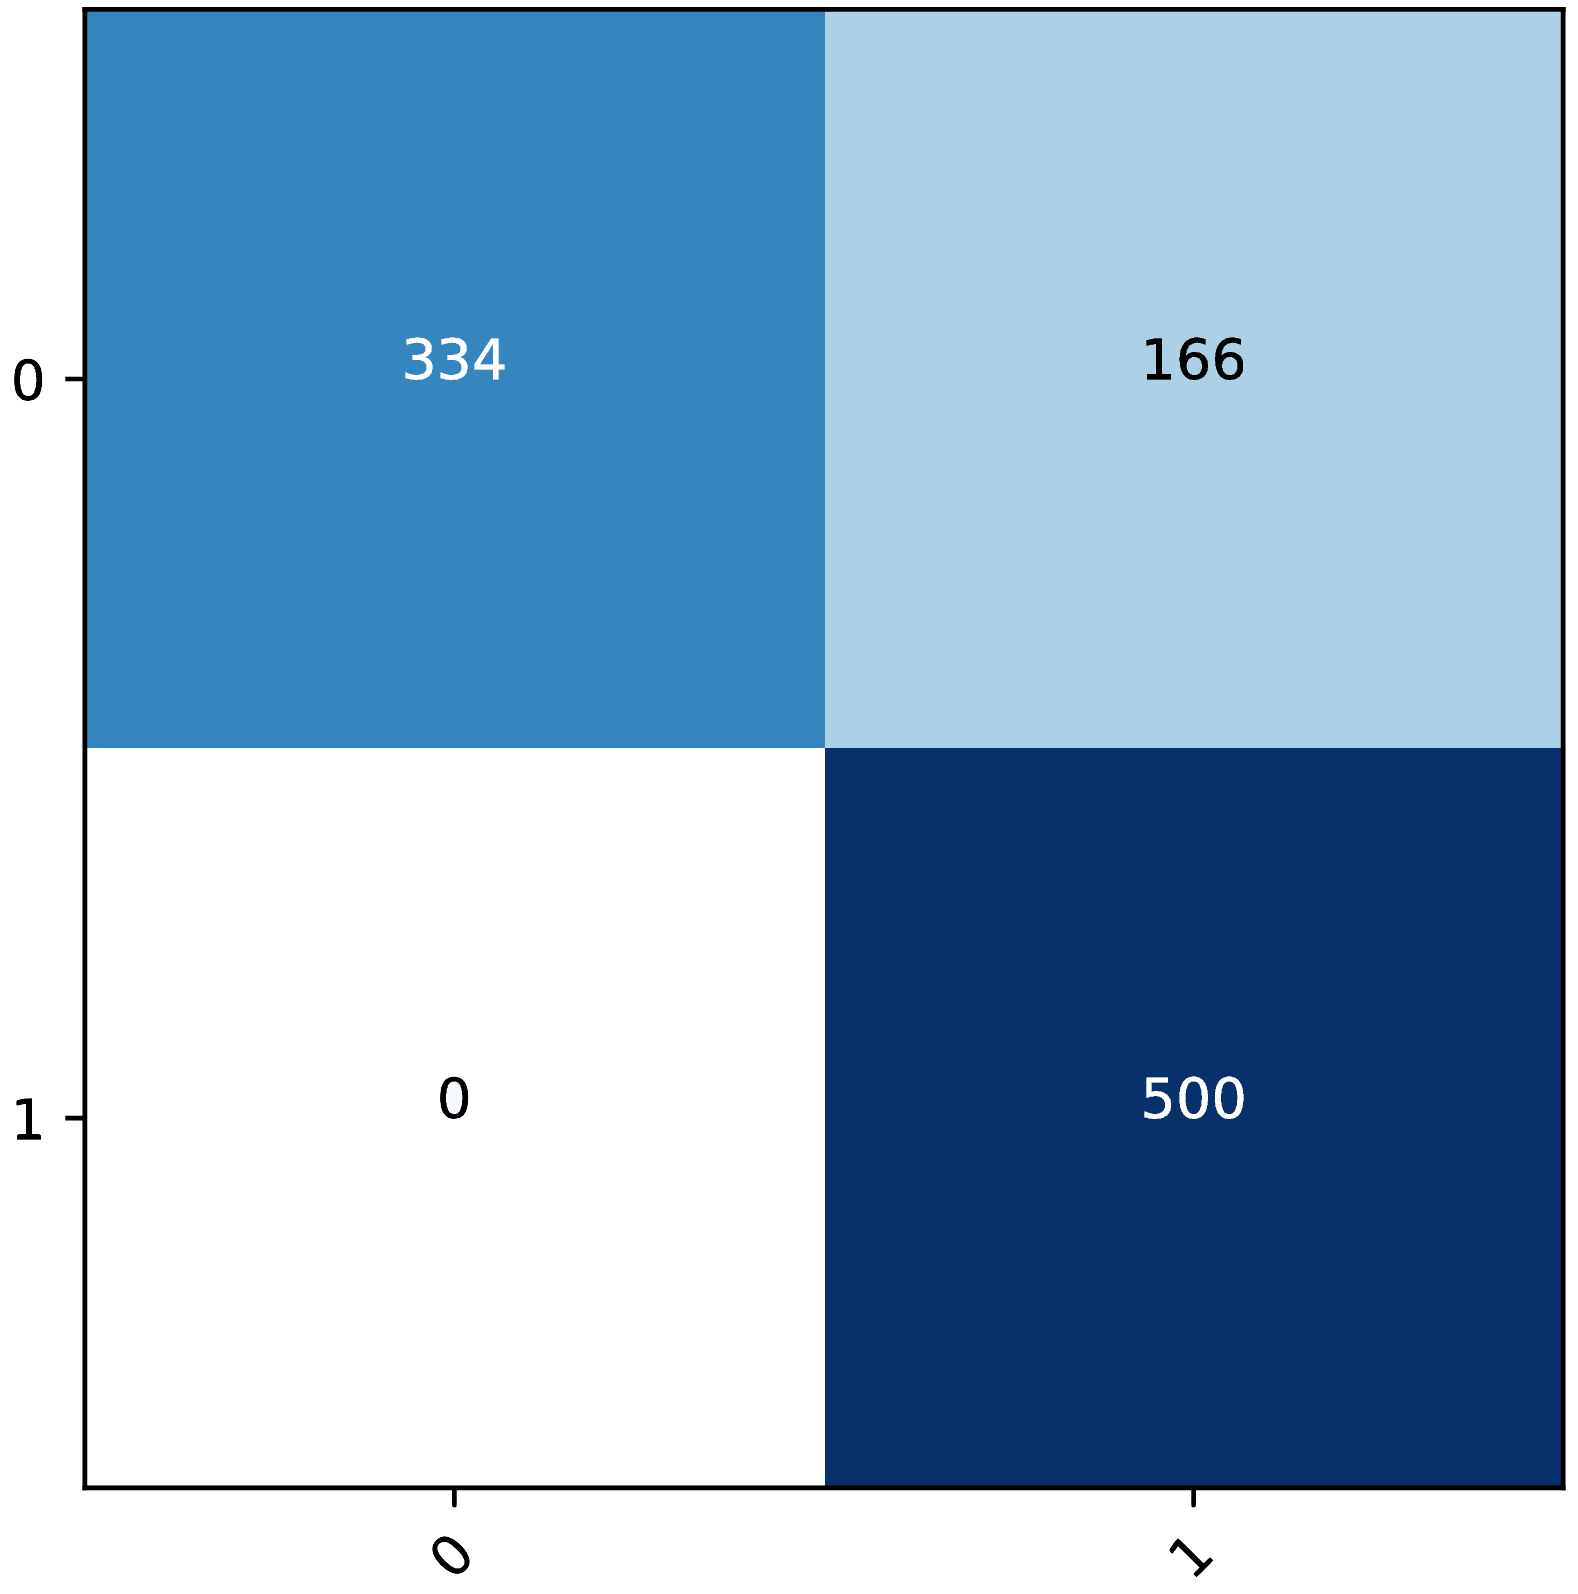
\includegraphics[height=.49\textheight, width=.99\textwidth, keepaspectratio]{circles_confusion_matrix.png}
    \end{minipage}
    \begin{minipage}{.49\textwidth}
        \centering
        \setlength\figureheight{.65\textheight}
        \setlength\figurewidth{1.2\textwidth}
        % This file was created by matplotlib2tikz v0.6.11.
\begin{tikzpicture}

\definecolor{color1}{rgb}{1,0.498039215686275,0.0549019607843137}
\definecolor{color0}{rgb}{0.12156862745098,0.466666666666667,0.705882352941177}
\pgfplotsset{ticks=none}
\begin{axis}[
xmin=-0.0501982678592688, xmax=1.05034339922085,
ymin=-0.0504608439109815, ymax=1.05026618150002,
width=\figurewidth,
height=\figureheight,
tick pos=left
]
\addplot [only marks, mark size=0.5pt, draw=color0, fill=color0, colormap/viridis]
table{%
x                      y
+8.107673525810242e-01 +1.892337948083878e-01
+8.530960679054260e-01 +1.469039320945740e-01
+5.719955563545227e-01 +4.280040860176086e-01
+7.959983944892883e-01 +2.040005326271057e-01
+9.753470420837402e-01 +2.465358190238476e-02
+6.053467392921448e-01 +3.946532905101776e-01
+5.478360652923584e-01 +4.521639645099640e-01
+7.786223888397217e-01 +2.213781774044037e-01
+8.989110589027405e-01 +1.010884493589401e-01
+8.333458900451660e-01 +1.666536778211594e-01
+8.551456332206726e-01 +1.448546051979065e-01
+7.666328549385071e-01 +2.333661913871765e-01
+9.347387552261353e-01 +6.526029109954834e-02
+7.566502094268799e-01 +2.433496713638306e-01
+7.612305283546448e-01 +2.387695163488388e-01
+8.390200138092041e-01 +1.609793305397034e-01
+7.577598094940186e-01 +2.422394752502441e-01
+9.903104901313782e-01 +9.690270759165287e-03
+5.116949081420898e-01 +4.883051812648773e-01
+8.223959207534790e-01 +1.776036322116852e-01
+9.418436288833618e-01 +5.815552547574043e-02
+9.971238970756531e-01 +2.875503618270159e-03
+7.505594491958618e-01 +2.494409978389740e-01
+9.109899997711182e-01 +8.900938928127289e-02
+6.610676050186157e-01 +3.389324545860291e-01
+7.180987596511841e-01 +2.819009423255920e-01
+9.579163193702698e-01 +4.208325967192650e-02
+6.661232113838196e-01 +3.338761031627655e-01
+5.341864228248596e-01 +4.658136665821075e-01
+7.353866100311279e-01 +2.646135687828064e-01
+5.591231584548950e-01 +4.408770799636841e-01
+8.556087613105774e-01 +1.443908065557480e-01
+7.357718944549561e-01 +2.642273604869843e-01
+9.338142871856689e-01 +6.618677079677582e-02
+6.239585876464844e-01 +3.760413825511932e-01
+6.396217942237854e-01 +3.603782355785370e-01
+5.595015883445740e-01 +4.404984712600708e-01
+8.682104349136353e-01 +1.317889839410782e-01
+7.405769824981689e-01 +2.594236433506012e-01
+7.930992245674133e-01 +2.068998366594315e-01
+7.639032602310181e-01 +2.360968142747879e-01
+9.017536044120789e-01 +9.824743121862411e-02
+7.247052192687988e-01 +2.752952277660370e-01
+7.894005775451660e-01 +2.105998396873474e-01
+7.460700869560242e-01 +2.539308965206146e-01
+7.863083481788635e-01 +2.136916667222977e-01
+9.156087636947632e-01 +8.439210057258606e-02
+9.268820285797119e-01 +7.311736047267914e-02
+8.638686537742615e-01 +1.361315697431564e-01
+5.954892635345459e-01 +4.045108854770660e-01
+9.482263326644897e-01 +5.177494138479233e-02
+5.512316823005676e-01 +4.487682580947876e-01
+7.795333266258240e-01 +2.204667925834656e-01
+9.249343276023865e-01 +7.506608217954636e-02
+7.639539837837219e-01 +2.360463291406631e-01
+7.944412827491760e-01 +2.055586278438568e-01
+5.249909758567810e-01 +4.750088751316071e-01
+9.784626960754395e-01 +2.153659611940384e-02
+8.582910895347595e-01 +1.417093425989151e-01
+7.975136041641235e-01 +2.024860978126526e-01
+8.745958805084229e-01 +1.254034787416458e-01
+9.676723480224609e-01 +3.232794627547264e-02
+9.596047401428223e-01 +4.039452970027924e-02
+8.159643411636353e-01 +1.840351223945618e-01
+5.628316402435303e-01 +4.371684789657593e-01
+8.582971096038818e-01 +1.417028754949570e-01
+7.578201889991760e-01 +2.421797215938568e-01
+9.565053582191467e-01 +4.349401965737343e-02
+8.950807452201843e-01 +1.049188226461411e-01
+9.353079199790955e-01 +6.469283252954483e-02
+5.384014844894409e-01 +4.615986943244934e-01
+9.123052358627319e-01 +8.769545704126358e-02
+5.054321885108948e-01 +4.945678412914276e-01
+5.953302979469299e-01 +4.046692550182343e-01
+7.268015146255493e-01 +2.731990516185760e-01
+7.252957820892334e-01 +2.747043967247009e-01
+7.862274050712585e-01 +2.137718796730042e-01
+8.026956319808960e-01 +1.973050534725189e-01
+9.431070089340210e-01 +5.689395591616631e-02
+8.133691549301147e-01 +1.866313815116882e-01
+5.682181715965271e-01 +4.317817986011505e-01
+6.403648257255554e-01 +3.596357107162476e-01
+7.677963972091675e-01 +2.322031855583191e-01
+7.644165158271790e-01 +2.355837672948837e-01
+1.000000000000000e+00 +6.026236367556725e-12
+8.393454551696777e-01 +1.606548279523849e-01
+7.730208635330200e-01 +2.269789725542068e-01
+9.377949237823486e-01 +6.220578029751778e-02
+8.636522889137268e-01 +1.363486647605896e-01
+5.854418277740479e-01 +4.145580232143402e-01
+7.714722156524658e-01 +2.285270839929581e-01
+9.391503930091858e-01 +6.084915623068810e-02
+7.384973764419556e-01 +2.615031898021698e-01
+7.961431741714478e-01 +2.038560807704926e-01
+7.005107998847961e-01 +2.994898855686188e-01
+7.998527288436890e-01 +2.001476138830185e-01
+9.343743920326233e-01 +6.562485545873642e-02
+8.681252002716064e-01 +1.318759769201279e-01
+9.762949347496033e-01 +2.370574511587620e-02
+5.555915236473083e-01 +4.444085359573364e-01
+9.439696669578552e-01 +5.603074654936790e-02
+9.661005139350891e-01 +3.390001878142357e-02
+8.577492237091064e-01 +1.422519534826279e-01
+7.864661216735840e-01 +2.135335505008698e-01
+9.271724224090576e-01 +7.282641530036926e-02
+9.027564525604248e-01 +9.724266827106476e-02
+9.071099758148193e-01 +9.289032965898514e-02
+9.573518633842468e-01 +4.264758154749870e-02
+7.979894876480103e-01 +2.020099461078644e-01
+9.541631340980530e-01 +4.583628475666046e-02
+7.152554988861084e-01 +2.847446799278259e-01
+7.198437452316284e-01 +2.801565825939178e-01
+7.380040884017944e-01 +2.619953453540802e-01
+9.748861193656921e-01 +2.511326782405376e-02
+9.095689654350281e-01 +9.043058753013611e-02
+9.293801784515381e-01 +7.062050700187683e-02
+9.455724954605103e-01 +5.442632734775543e-02
+8.230216503143311e-01 +1.769773364067078e-01
+7.903794050216675e-01 +2.096208781003952e-01
+7.462570071220398e-01 +2.537427842617035e-01
+8.689644336700439e-01 +1.310366988182068e-01
+6.952211856842041e-01 +3.047786056995392e-01
+8.686452507972717e-01 +1.313542574644089e-01
+7.520751357078552e-01 +2.479248195886612e-01
+8.433830738067627e-01 +1.566174030303955e-01
+7.809110879898071e-01 +2.190895229578018e-01
+8.536674976348877e-01 +1.463334262371063e-01
+7.675865292549133e-01 +2.324123978614807e-01
+7.040778398513794e-01 +2.959232032299042e-01
+5.875548720359802e-01 +4.124450981616974e-01
+9.562688469886780e-01 +4.373042657971382e-02
+7.805963754653931e-01 +2.194035500288010e-01
+8.822529315948486e-01 +1.177473738789558e-01
+7.475408315658569e-01 +2.524586021900177e-01
+9.189298748970032e-01 +8.107087016105652e-02
+7.496438622474670e-01 +2.503566443920135e-01
+1.000000000000000e+00 +1.121198945318314e-12
+8.800432085990906e-01 +1.199562549591064e-01
+8.050615191459656e-01 +1.949380636215210e-01
+7.166774272918701e-01 +2.833232581615448e-01
+5.130383968353271e-01 +4.869616329669952e-01
+7.121436595916748e-01 +2.878556549549103e-01
+7.427214980125427e-01 +2.572785913944244e-01
+6.010770201683044e-01 +3.989234566688538e-01
+5.717163681983948e-01 +4.282836616039276e-01
+9.323449730873108e-01 +6.765446811914444e-02
+5.547788143157959e-01 +4.452213048934937e-01
+7.873612046241760e-01 +2.126388102769852e-01
+7.917250990867615e-01 +2.082748562097549e-01
+7.620392441749573e-01 +2.379608005285263e-01
+1.000000000000000e+00 +1.797687324521513e-12
+8.585151433944702e-01 +1.414842754602432e-01
+8.927327990531921e-01 +1.072672903537750e-01
+5.633087754249573e-01 +4.366912543773651e-01
+6.610295176506042e-01 +3.389705717563629e-01
+8.137437701225281e-01 +1.862557828426361e-01
+8.106360435485840e-01 +1.893641352653503e-01
+9.381353855133057e-01 +6.186393648386002e-02
+7.630997300148010e-01 +2.369003146886826e-01
+8.268536925315857e-01 +1.731459647417068e-01
+9.116994738578796e-01 +8.830036222934723e-02
+8.883563280105591e-01 +1.116444841027260e-01
+6.821103096008301e-01 +3.178897798061371e-01
+6.374137401580811e-01 +3.625856637954712e-01
+8.365408182144165e-01 +1.634586155414581e-01
+9.998912215232849e-01 +1.095049738069065e-04
+7.614569067955017e-01 +2.385426014661789e-01
+8.177026510238647e-01 +1.822978407144547e-01
+8.969802260398865e-01 +1.030200645327568e-01
+9.294941425323486e-01 +7.050658017396927e-02
+8.518807291984558e-01 +1.481189876794815e-01
+9.294814467430115e-01 +7.051850110292435e-02
+8.611680865287781e-01 +1.388313919305801e-01
+8.144330382347107e-01 +1.855666190385818e-01
+7.312366366386414e-01 +2.687630355358124e-01
+8.567268848419189e-01 +1.432740539312363e-01
+9.777913093566895e-01 +2.220810577273369e-02
+6.909400224685669e-01 +3.090609312057495e-01
+9.017564654350281e-01 +9.824283421039581e-02
+8.566743731498718e-01 +1.433251053094864e-01
+9.530767202377319e-01 +4.692416265606880e-02
+9.100501537322998e-01 +8.994899690151215e-02
+8.025359511375427e-01 +1.974639743566513e-01
+8.526486158370972e-01 +1.473510116338730e-01
+7.347977161407471e-01 +2.652021050453186e-01
+9.587001204490662e-01 +4.130047932267189e-02
+7.808457016944885e-01 +2.191543430089951e-01
+9.211905002593994e-01 +7.880889624357224e-02
+7.709656357765198e-01 +2.290342450141907e-01
+5.297623276710510e-01 +4.702377021312714e-01
+7.776055335998535e-01 +2.223949283361435e-01
+7.977606058120728e-01 +2.022387832403183e-01
+7.638275027275085e-01 +2.361722439527512e-01
+9.360752701759338e-01 +6.392475217580795e-02
+8.134483098983765e-01 +1.865518987178802e-01
+9.764271378517151e-01 +2.357236295938492e-02
+9.028447866439819e-01 +9.715564548969269e-02
+5.198909640312195e-01 +4.801089465618134e-01
+8.845040202140808e-01 +1.154965683817863e-01
+7.786819934844971e-01 +2.213173508644104e-01
+8.287506699562073e-01 +1.712487190961838e-01
+7.313987016677856e-01 +2.686023414134979e-01
+8.063509464263916e-01 +1.936485469341278e-01
+8.041082620620728e-01 +1.958911865949631e-01
+9.879093766212463e-01 +1.208981126546860e-02
+8.975296616554260e-01 +1.024700477719307e-01
+8.728692531585693e-01 +1.271305680274963e-01
+5.631253719329834e-01 +4.368746578693390e-01
+8.543464541435242e-01 +1.456546932458878e-01
+6.606301665306091e-01 +3.393689692020416e-01
+5.211527347564697e-01 +4.788472056388855e-01
+9.070337414741516e-01 +9.296648204326630e-02
+8.367688655853271e-01 +1.632316559553146e-01
+9.496021866798401e-01 +5.039786919951439e-02
+9.095153212547302e-01 +9.048464894294739e-02
+7.492286562919617e-01 +2.507723569869995e-01
+6.169698238372803e-01 +3.830303251743317e-01
+1.000000000000000e+00 +1.571182528699311e-12
+8.289946913719177e-01 +1.710054427385330e-01
+9.898625016212463e-01 +1.013694982975721e-02
+9.243905544281006e-01 +7.561015337705612e-02
+8.676478862762451e-01 +1.323518604040146e-01
+9.731542468070984e-01 +2.684521488845348e-02
+8.937836289405823e-01 +1.062163561582565e-01
+8.934251666069031e-01 +1.065740883350372e-01
+9.112548232078552e-01 +8.874512463808060e-02
+8.184003233909607e-01 +1.815994828939438e-01
+9.948579668998718e-01 +5.141528788954020e-03
+5.775861144065857e-01 +4.224142730236053e-01
+7.430921196937561e-01 +2.569082975387573e-01
+9.459787607192993e-01 +5.401996150612831e-02
+8.439948558807373e-01 +1.560046672821045e-01
+5.850058794021606e-01 +4.149944782257080e-01
+8.729684352874756e-01 +1.270313858985901e-01
+9.613794088363647e-01 +3.862165287137032e-02
+8.281455039978027e-01 +1.718546897172928e-01
+8.775869011878967e-01 +1.224126741290092e-01
+9.149601459503174e-01 +8.504068106412888e-02
+9.046453237533569e-01 +9.535540640354156e-02
+7.252318859100342e-01 +2.747682631015778e-01
+8.012464642524719e-01 +1.987539827823639e-01
+7.862213850021362e-01 +2.137789130210876e-01
+8.131638169288635e-01 +1.868360489606857e-01
+6.710544824600220e-01 +3.289456069469452e-01
+6.796679496765137e-01 +3.203319609165192e-01
+7.151563167572021e-01 +2.848439514636993e-01
+8.059995770454407e-01 +1.940008699893951e-01
+9.100320339202881e-01 +8.996859192848206e-02
+7.092410326004028e-01 +2.907585203647614e-01
+9.843366742134094e-01 +1.566394418478012e-02
+9.531154036521912e-01 +4.688496887683868e-02
+7.222111225128174e-01 +2.777881920337677e-01
+7.212151288986206e-01 +2.787839174270630e-01
+9.708118438720703e-01 +2.918793633580208e-02
+7.354463934898376e-01 +2.645530998706818e-01
+7.251121997833252e-01 +2.748885750770569e-01
+9.895683526992798e-01 +1.043249573558569e-02
+5.907935500144958e-01 +4.092065095901489e-01
+8.895034193992615e-01 +1.104965507984161e-01
+7.352668642997742e-01 +2.647341489791870e-01
+7.459264993667603e-01 +2.540727555751801e-01
+8.281104564666748e-01 +1.718885749578476e-01
+8.241934776306152e-01 +1.758067458868027e-01
+8.846659064292908e-01 +1.153345331549644e-01
+8.998952507972717e-01 +1.001039817929268e-01
+9.268316030502319e-01 +7.316878437995911e-02
+9.073892831802368e-01 +9.260997176170349e-02
+7.703964710235596e-01 +2.296028584241867e-01
+9.912084937095642e-01 +8.792761713266373e-03
+7.091597914695740e-01 +2.908402681350708e-01
+8.882953524589539e-01 +1.117054447531700e-01
+7.932227849960327e-01 +2.067775577306747e-01
+9.410553574562073e-01 +5.894457176327705e-02
+9.045055508613586e-01 +9.549341350793839e-02
+9.816412925720215e-01 +1.835943013429642e-02
+7.678072452545166e-01 +2.321923822164536e-01
+9.451503157615662e-01 +5.485009774565697e-02
+7.061663866043091e-01 +2.938331961631775e-01
+8.785558342933655e-01 +1.214437410235405e-01
+5.179165005683899e-01 +4.820835888385773e-01
+8.799540996551514e-01 +1.200454235076904e-01
+9.720286726951599e-01 +2.797191776335239e-02
+9.839700460433960e-01 +1.603113673627377e-02
+8.282576203346252e-01 +1.717415452003479e-01
+8.894502520561218e-01 +1.105490401387215e-01
+5.522692203521729e-01 +4.477306604385376e-01
+8.238877654075623e-01 +1.761131137609482e-01
+8.052675724029541e-01 +1.947319209575653e-01
+7.800621986389160e-01 +2.199381440877914e-01
+8.486731648445129e-01 +1.513268798589706e-01
+9.824907183647156e-01 +1.750861853361130e-02
+7.610092759132385e-01 +2.389907687902451e-01
+7.791746258735657e-01 +2.208257168531418e-01
+8.728665113449097e-01 +1.271326541900635e-01
+9.787163734436035e-01 +2.128302119672298e-02
+5.125932693481445e-01 +4.874066412448883e-01
+8.407767415046692e-01 +1.592233031988144e-01
+8.354104757308960e-01 +1.645899564027786e-01
+5.592458248138428e-01 +4.407542347908020e-01
+7.049440145492554e-01 +2.950558960437775e-01
+7.207192182540894e-01 +2.792797386646271e-01
+7.314941883087158e-01 +2.685055434703827e-01
+7.037889957427979e-01 +2.962107360363007e-01
+8.126525282859802e-01 +1.873474270105362e-01
+9.124748706817627e-01 +8.752623200416565e-02
+7.120469808578491e-01 +2.879528403282166e-01
+9.032461643218994e-01 +9.675312042236328e-02
+7.211609482765198e-01 +2.788389921188354e-01
+5.298603177070618e-01 +4.701397716999054e-01
+8.085175156593323e-01 +1.914819329977036e-01
+9.393239617347717e-01 +6.067558377981186e-02
+9.563062787055969e-01 +4.369422420859337e-02
+9.079686999320984e-01 +9.203106909990311e-02
+9.180430769920349e-01 +8.195689320564270e-02
+8.156738877296448e-01 +1.843261569738388e-01
+9.544988274574280e-01 +4.550044611096382e-02
+9.133352041244507e-01 +8.666556328535080e-02
+7.552825808525085e-01 +2.447171658277512e-01
+8.597564101219177e-01 +1.402437537908554e-01
+5.474272966384888e-01 +4.525729119777679e-01
+5.459071993827820e-01 +4.540925920009613e-01
+9.549962878227234e-01 +4.500298202037811e-02
+9.106667041778564e-01 +8.933407068252563e-02
+7.392858266830444e-01 +2.607136070728302e-01
+8.785172104835510e-01 +1.214825883507729e-01
+8.448840379714966e-01 +1.551163047552109e-01
+8.375627994537354e-01 +1.624364852905273e-01
+8.839271068572998e-01 +1.160719469189644e-01
+9.121502041816711e-01 +8.784907311201096e-02
+7.284649014472961e-01 +2.715353369712830e-01
+8.112820982933044e-01 +1.887175440788269e-01
+8.791269659996033e-01 +1.208736896514893e-01
+7.138187885284424e-01 +2.861806154251099e-01
+9.361421465873718e-01 +6.385708600282669e-02
};
\addplot [only marks, mark size=0.5pt, draw=color1, fill=color1, colormap/viridis]
table{%
x                      y
+3.473128974437714e-01 +6.526871323585510e-01
+3.328319787979126e-01 +6.671677231788635e-01
+1.745279133319855e-01 +8.254722356796265e-01
+9.046970307826996e-02 +9.095305800437927e-01
+2.781505286693573e-01 +7.218483686447144e-01
+2.908645570278168e-01 +7.091362476348877e-01
+3.011241853237152e-01 +6.988756656646729e-01
+1.722266227006912e-01 +8.277738690376282e-01
+3.051638603210449e-01 +6.948361992835999e-01
+1.229820176959038e-01 +8.770190477371216e-01
+3.294600248336792e-01 +6.705399155616760e-01
+3.190502822399139e-01 +6.809496879577637e-01
+3.259161710739136e-01 +6.740840673446655e-01
+3.325654268264771e-01 +6.674346327781677e-01
+3.144039809703827e-01 +6.855959892272949e-01
+3.323359787464142e-01 +6.676638126373291e-01
+4.231959208846092e-02 +9.576799273490906e-01
+3.083514869213104e-01 +6.916494965553284e-01
+8.540099859237671e-02 +9.145987033843994e-01
+3.083343803882599e-01 +6.916655898094177e-01
+3.046784698963165e-01 +6.953208446502686e-01
+2.953510582447052e-01 +7.046482563018799e-01
+3.201927244663239e-01 +6.798066496849060e-01
+3.078407943248749e-01 +6.921587586402893e-01
+3.151417970657349e-01 +6.848574876785278e-01
+3.362103700637817e-01 +6.637887358665466e-01
+2.959402799606323e-01 +7.040600776672363e-01
+7.557299733161926e-02 +9.244258403778076e-01
+3.016473054885864e-01 +6.983524560928345e-01
+3.114585578441620e-01 +6.885411143302917e-01
+3.324656784534454e-01 +6.675341129302979e-01
+1.140893623232841e-02 +9.885917901992798e-01
+2.849807441234589e-01 +7.150192260742188e-01
+4.891002178192139e-01 +5.108997225761414e-01
+3.002399504184723e-01 +6.997601985931396e-01
+2.956556975841522e-01 +7.043454647064209e-01
+3.241348266601562e-01 +6.758651733398438e-01
+3.107265532016754e-01 +6.892734766006470e-01
+3.197845220565796e-01 +6.802147030830383e-01
+3.054657280445099e-01 +6.945342421531677e-01
+5.419857427477837e-02 +9.458009600639343e-01
+3.113193213939667e-01 +6.886816620826721e-01
+8.875073492527008e-02 +9.112493395805359e-01
+1.456126570701599e-01 +8.543875217437744e-01
+2.974819242954254e-01 +7.025179266929626e-01
+3.004469573497772e-01 +6.995537281036377e-01
+3.150792121887207e-01 +6.849210262298584e-01
+3.330951631069183e-01 +6.669048070907593e-01
+3.061480224132538e-01 +6.938520073890686e-01
+3.203807771205902e-01 +6.796190738677979e-01
+3.317070305347443e-01 +6.682927608489990e-01
+2.723602950572968e-01 +7.276389598846436e-01
+3.075328767299652e-01 +6.924669742584229e-01
+1.392335742712021e-01 +8.607662320137024e-01
+2.996277213096619e-01 +7.003715038299561e-01
+3.309120535850525e-01 +6.690874695777893e-01
+3.004322350025177e-01 +6.995670199394226e-01
+2.945860624313354e-01 +7.054138779640198e-01
+3.245468437671661e-01 +6.754531264305115e-01
+3.130720853805542e-01 +6.869278550148010e-01
+3.278888761997223e-01 +6.721112728118896e-01
+3.202434480190277e-01 +6.797564029693604e-01
+1.198825612664223e-01 +8.801186084747314e-01
+3.025879859924316e-01 +6.974112987518311e-01
+3.307499587535858e-01 +6.692502498626709e-01
+3.225535154342651e-01 +6.774471998214722e-01
+3.220534622669220e-01 +6.779472827911377e-01
+3.194599449634552e-01 +6.805392503738403e-01
+3.005385994911194e-01 +6.994621753692627e-01
+3.236522376537323e-01 +6.763467192649841e-01
+3.168889284133911e-01 +6.831103563308716e-01
+1.943784952163696e-01 +8.056212663650513e-01
+6.555847078561783e-02 +9.344407916069031e-01
+3.169455826282501e-01 +6.830549836158752e-01
+3.172726333141327e-01 +6.827273368835449e-01
+3.163684606552124e-01 +6.836316585540771e-01
+3.212132155895233e-01 +6.787869930267334e-01
+3.107877075672150e-01 +6.892122626304626e-01
+2.132509648799896e-01 +7.867500185966492e-01
+2.973102629184723e-01 +7.026898860931396e-01
+3.312777578830719e-01 +6.687231659889221e-01
+1.863119006156921e-01 +8.136879205703735e-01
+6.138789281249046e-02 +9.386131763458252e-01
+3.286052942276001e-01 +6.713945865631104e-01
+3.347687125205994e-01 +6.652305722236633e-01
+2.833825349807739e-01 +7.166171073913574e-01
+3.263163864612579e-01 +6.736834049224854e-01
+3.169741332530975e-01 +6.830258369445801e-01
+7.129910588264465e-02 +9.287012219429016e-01
+7.931946963071823e-02 +9.206798076629639e-01
+2.875551879405975e-01 +7.124449014663696e-01
+1.204004511237144e-01 +8.795999884605408e-01
+3.234426081180573e-01 +6.765567064285278e-01
+2.930623292922974e-01 +7.069370150566101e-01
+2.886848151683807e-01 +7.113156318664551e-01
+2.075555920600891e-01 +7.924447059631348e-01
+2.984718382358551e-01 +7.015276551246643e-01
+2.985687553882599e-01 +7.014312148094177e-01
+3.457145392894745e-01 +6.542856097221375e-01
+3.247474730014801e-01 +6.752519011497498e-01
+1.076686084270477e-01 +8.923317790031433e-01
+3.233145475387573e-01 +6.766856312751770e-01
+3.099250495433807e-01 +6.900752186775208e-01
+1.260109096765518e-01 +8.739899992942810e-01
+3.069405555725098e-01 +6.930590271949768e-01
+3.119983375072479e-01 +6.880026459693909e-01
+3.350558578968048e-01 +6.649440526962280e-01
+3.286117911338806e-01 +6.713874936103821e-01
+3.089441955089569e-01 +6.910555362701416e-01
+3.403181433677673e-01 +6.596824526786804e-01
+3.013367950916290e-01 +6.986625194549561e-01
+3.265148103237152e-01 +6.734850406646729e-01
+3.256624937057495e-01 +6.743384599685669e-01
+3.086472749710083e-01 +6.913527846336365e-01
+3.268278837203979e-01 +6.731720566749573e-01
+3.307709991931915e-01 +6.692283153533936e-01
+3.290447294712067e-01 +6.709553003311157e-01
+2.943834960460663e-01 +7.056165933609009e-01
+9.763495624065399e-02 +9.023659229278564e-01
+3.249439299106598e-01 +6.750562191009521e-01
+5.499805510044098e-02 +9.450016617774963e-01
+2.185077518224716e-01 +7.814933657646179e-01
+2.851213812828064e-01 +7.148786783218384e-01
+3.109049797058105e-01 +6.890947818756104e-01
+3.231984376907349e-01 +6.768008470535278e-01
+3.150086402893066e-01 +6.849906444549561e-01
+3.259105980396271e-01 +6.740884184837341e-01
+3.156047165393829e-01 +6.843950748443604e-01
+3.158450424671173e-01 +6.841549873352051e-01
+2.908596396446228e-01 +7.091402411460876e-01
+2.965641915798187e-01 +7.034351229667664e-01
+3.223360776901245e-01 +6.776648759841919e-01
+1.435048431158066e-01 +8.564959168434143e-01
+1.202821508049965e-01 +8.797175884246826e-01
+3.108424842357635e-01 +6.891582608222961e-01
+9.146635979413986e-02 +9.085333347320557e-01
+2.858868837356567e-01 +7.141121625900269e-01
+1.056082621216774e-01 +8.943918347358704e-01
+4.154442250728607e-02 +9.584560394287109e-01
+3.048973381519318e-01 +6.951023936271667e-01
+3.254198729991913e-01 +6.745800971984863e-01
+2.981548011302948e-01 +7.018459439277649e-01
+3.187980353832245e-01 +6.812022328376770e-01
+2.994861304759979e-01 +7.005149126052856e-01
+3.357526063919067e-01 +6.642464995384216e-01
+3.247183561325073e-01 +6.752818226814270e-01
+3.134273588657379e-01 +6.865725517272949e-01
+3.131351470947266e-01 +6.868640780448914e-01
+1.632089763879776e-01 +8.367913961410522e-01
+1.998079717159271e-01 +8.001930117607117e-01
+3.147983849048615e-01 +6.852008700370789e-01
+2.943916022777557e-01 +7.056087255477905e-01
+3.184221982955933e-01 +6.815787553787231e-01
+2.991791963577271e-01 +7.008208632469177e-01
+3.011603057384491e-01 +6.988400816917419e-01
+3.138790428638458e-01 +6.861199736595154e-01
+8.586943894624710e-02 +9.141309857368469e-01
+3.136630356311798e-01 +6.863369941711426e-01
+3.186531364917755e-01 +6.813465952873230e-01
+3.116091787815094e-01 +6.883918046951294e-01
+3.256583511829376e-01 +6.743422150611877e-01
+2.722144424915314e-01 +7.277858853340149e-01
+3.142604529857635e-01 +6.857402920722961e-01
+6.195732206106186e-02 +9.380422234535217e-01
+3.164218962192535e-01 +6.835782527923584e-01
+2.963577210903168e-01 +7.036430835723877e-01
+3.214186429977417e-01 +6.785812973976135e-01
+3.269654512405396e-01 +6.730346083641052e-01
+2.969833314418793e-01 +7.030174732208252e-01
+3.274213373661041e-01 +6.725777387619019e-01
+2.990454435348511e-01 +7.009547948837280e-01
+3.135490715503693e-01 +6.864506602287292e-01
+6.990732252597809e-02 +9.300920367240906e-01
+2.991409599781036e-01 +7.008590102195740e-01
+2.069550156593323e-01 +7.930449843406677e-01
+2.923292815685272e-01 +7.076714038848877e-01
+2.953658699989319e-01 +7.046349048614502e-01
+3.222841918468475e-01 +6.777161955833435e-01
+7.606305927038193e-02 +9.239369034767151e-01
+3.006702363491058e-01 +6.993299126625061e-01
+3.246245086193085e-01 +6.753761768341064e-01
+3.194312751293182e-01 +6.805689334869385e-01
+3.094328939914703e-01 +6.905670762062073e-01
+3.165412843227386e-01 +6.834592223167419e-01
+3.106750547885895e-01 +6.893242001533508e-01
+3.030565977096558e-01 +6.969443559646606e-01
+3.261374235153198e-01 +6.738627552986145e-01
+2.977637350559235e-01 +7.022365331649780e-01
+3.098869025707245e-01 +6.901133656501770e-01
+3.104567527770996e-01 +6.895439624786377e-01
+3.281483352184296e-01 +6.718518733978271e-01
+3.217448890209198e-01 +6.782559156417847e-01
+3.131203651428223e-01 +6.868790984153748e-01
+3.139019384980202e-02 +9.686102867126465e-01
+3.050556480884552e-01 +6.949436068534851e-01
+1.172132417559624e-01 +8.827874064445496e-01
+3.081817924976349e-01 +6.918181777000427e-01
+3.080252408981323e-01 +6.919749975204468e-01
+1.627166718244553e-01 +8.372830152511597e-01
+3.180979490280151e-01 +6.819027662277222e-01
+3.163052797317505e-01 +6.836937665939331e-01
+3.101992309093475e-01 +6.898007988929749e-01
+2.968354523181915e-01 +7.031633853912354e-01
+3.255638182163239e-01 +6.744355559349060e-01
+3.171859085559845e-01 +6.828148365020752e-01
+3.134079873561859e-01 +6.865920424461365e-01
+2.908877134323120e-01 +7.091132402420044e-01
+3.045201003551483e-01 +6.954801082611084e-01
+3.254432380199432e-01 +6.745569705963135e-01
+3.156871497631073e-01 +6.843135952949524e-01
+3.013553917407990e-01 +6.986438632011414e-01
+9.199523180723190e-02 +9.080048203468323e-01
+3.056827485561371e-01 +6.943172216415405e-01
+1.965903639793396e-01 +8.034104108810425e-01
+5.341496318578720e-02 +9.465860128402710e-01
+3.080865144729614e-01 +6.919132471084595e-01
+3.252010047435760e-01 +6.747979521751404e-01
+3.262733817100525e-01 +6.737260222434998e-01
+3.182883262634277e-01 +6.817122101783752e-01
+3.260159790515900e-01 +6.739840507507324e-01
+3.020214736461639e-01 +6.979784369468689e-01
+3.053306639194489e-01 +6.946688294410706e-01
+9.308059513568878e-02 +9.069193005561829e-01
+2.927589118480682e-01 +7.072414159774780e-01
+3.192138969898224e-01 +6.807860732078552e-01
+3.273487985134125e-01 +6.726523041725159e-01
+1.186742037534714e-01 +8.813253045082092e-01
+3.078536689281464e-01 +6.921463608741760e-01
+3.095012009143829e-01 +6.904985904693604e-01
+3.236886262893677e-01 +6.763111948966980e-01
+7.094672322273254e-02 +9.290537238121033e-01
+3.171748816967010e-01 +6.828258633613586e-01
+3.304654657840729e-01 +6.695336103439331e-01
+3.094058930873871e-01 +6.905941963195801e-01
+6.999441981315613e-02 +9.300059676170349e-01
+3.295121490955353e-01 +6.704871654510498e-01
+2.845092415809631e-01 +7.154915332794189e-01
+3.169307410717010e-01 +6.830700039863586e-01
+4.875961288376696e-13 +1.000000000000000e+00
+3.112163841724396e-01 +6.887826323509216e-01
+3.517747819423676e-01 +6.482246518135071e-01
+3.113268911838531e-01 +6.886740326881409e-01
+2.966939210891724e-01 +7.033054232597351e-01
+2.970623075962067e-01 +7.029377222061157e-01
+4.366546124219894e-02 +9.563350081443787e-01
+3.088665306568146e-01 +6.911324858665466e-01
+5.200400948524475e-02 +9.479960799217224e-01
+3.157120943069458e-01 +6.842879652976990e-01
+3.327349126338959e-01 +6.672660112380981e-01
+3.158721625804901e-01 +6.841278672218323e-01
+3.129029273986816e-01 +6.870963573455811e-01
+3.195705711841583e-01 +6.804284453392029e-01
+3.165440261363983e-01 +6.834561824798584e-01
+1.167249903082848e-01 +8.832752704620361e-01
+3.283743560314178e-01 +6.716262102127075e-01
+3.137473762035370e-01 +6.862528920173645e-01
+3.196797072887421e-01 +6.803205013275146e-01
+3.209423720836639e-01 +6.790575981140137e-01
+3.050766289234161e-01 +6.949233412742615e-01
+1.007280647754669e-01 +8.992713093757629e-01
+1.260703057050705e-01 +8.739297389984131e-01
+6.549704074859619e-02 +9.345021843910217e-01
+3.646177798509598e-02 +9.635389447212219e-01
+3.005643188953400e-01 +6.994356513023376e-01
+3.135609626770020e-01 +6.864392757415771e-01
+3.146723806858063e-01 +6.853283643722534e-01
+7.347764819860458e-02 +9.265218377113342e-01
+3.074397742748260e-01 +6.925609707832336e-01
+1.413071304559708e-01 +8.586933016777039e-01
+8.036220818758011e-02 +9.196388721466064e-01
+3.273962736129761e-01 +6.726038455963135e-01
+3.282741308212280e-01 +6.717258691787720e-01
+2.816907167434692e-01 +7.183083295822144e-01
+3.000088036060333e-01 +6.999901533126831e-01
+3.165898323059082e-01 +6.834104061126709e-01
+3.217872679233551e-01 +6.782121062278748e-01
+4.902916029095650e-02 +9.509714245796204e-01
+7.860431075096130e-02 +9.213948845863342e-01
+3.046115934848785e-01 +6.953885555267334e-01
+3.198798894882202e-01 +6.801194548606873e-01
+3.073697388172150e-01 +6.926302313804626e-01
+3.062783479690552e-01 +6.937212944030762e-01
+3.278274834156036e-01 +6.721724867820740e-01
+3.034158051013947e-01 +6.965838074684143e-01
+3.184790909290314e-01 +6.815214753150940e-01
+3.278403878211975e-01 +6.721602082252502e-01
+3.174096345901489e-01 +6.825901865959167e-01
+2.975658774375916e-01 +7.024340033531189e-01
+3.285751044750214e-01 +6.714249253273010e-01
+3.042998313903809e-01 +6.957008838653564e-01
+3.096748292446136e-01 +6.903256773948669e-01
+3.162407577037811e-01 +6.837586760520935e-01
+3.227596282958984e-01 +6.772393584251404e-01
+2.886909544467926e-01 +7.113085985183716e-01
+3.275551199913025e-01 +6.724442839622498e-01
+2.994407713413239e-01 +7.005587220191956e-01
+2.984026670455933e-01 +7.015982866287231e-01
+3.203015029430389e-01 +6.796984672546387e-01
+3.203605711460114e-01 +6.796388030052185e-01
+2.995720207691193e-01 +7.004276514053345e-01
+2.044371068477631e-01 +7.955628037452698e-01
+4.164386689662933e-01 +5.835611820220947e-01
+3.266029655933380e-01 +6.733968257904053e-01
+3.120899498462677e-01 +6.879093050956726e-01
+4.623428732156754e-02 +9.537658095359802e-01
+3.227844536304474e-01 +6.772155165672302e-01
+3.197478950023651e-01 +6.802521347999573e-01
+3.076077401638031e-01 +6.923913359642029e-01
+1.274185031652451e-01 +8.725814819335938e-01
+2.956848442554474e-01 +7.043151259422302e-01
+3.360495865345001e-01 +6.639510393142700e-01
+1.171305254101753e-01 +8.828686475753784e-01
+1.699865460395813e-01 +8.300141692161560e-01
+1.460044234991074e-01 +8.539960980415344e-01
+4.230834543704987e-02 +9.576925039291382e-01
+3.051333129405975e-01 +6.948667168617249e-01
+3.111949265003204e-01 +6.888048648834229e-01
+4.230456799268723e-02 +9.576950669288635e-01
+3.158107101917267e-01 +6.841890811920166e-01
+3.057122230529785e-01 +6.942873597145081e-01
+3.128758370876312e-01 +6.871234774589539e-01
+9.225283563137054e-02 +9.077460765838623e-01
+2.983341515064240e-01 +7.016651034355164e-01
+1.122506633400917e-01 +8.877488970756531e-01
+6.500735133886337e-02 +9.349920749664307e-01
+3.222256898880005e-01 +6.777733564376831e-01
+6.158985942602158e-02 +9.384098649024963e-01
+3.093075752258301e-01 +6.906923651695251e-01
+2.661094963550568e-01 +7.338899970054626e-01
+4.548665881156921e-02 +9.545134902000427e-01
+6.283188611268997e-02 +9.371669292449951e-01
+3.168102502822876e-01 +6.831894516944885e-01
+2.999339103698730e-01 +7.000658512115479e-01
+3.113437592983246e-01 +6.886563301086426e-01
+2.873626649379730e-01 +7.126381397247314e-01
+3.156657516956329e-01 +6.843340396881104e-01
+3.221169710159302e-01 +6.778828501701355e-01
+3.044032156467438e-01 +6.955974698066711e-01
+3.129409849643707e-01 +6.870582699775696e-01
+1.975599527359009e-01 +8.024397492408752e-01
+3.032402992248535e-01 +6.967592835426331e-01
+3.014754951000214e-01 +6.985244750976562e-01
+6.053403764963150e-02 +9.394662976264954e-01
+3.116012513637543e-01 +6.883994340896606e-01
+3.264104127883911e-01 +6.735888123512268e-01
+2.229309529066086e-01 +7.770690321922302e-01
+3.008784055709839e-01 +6.991223692893982e-01
+3.167835474014282e-01 +6.832165718078613e-01
+3.142834007740021e-01 +6.857156157493591e-01
+3.180117607116699e-01 +6.819882392883301e-01
+1.171920076012611e-01 +8.828074932098389e-01
+3.209137022495270e-01 +6.790855526924133e-01
+2.936559021472931e-01 +7.063443660736084e-01
+3.144469559192657e-01 +6.855537891387939e-01
+3.256510198116302e-01 +6.743496656417847e-01
+3.078494071960449e-01 +6.921506524085999e-01
+3.081717491149902e-01 +6.918286681175232e-01
+3.076647520065308e-01 +6.923362016677856e-01
+3.025722205638885e-01 +6.974285244941711e-01
+1.420710235834122e-01 +8.579282164573669e-01
+3.193584382534027e-01 +6.806414127349854e-01
+2.934337258338928e-01 +7.065660953521729e-01
+3.209148347377777e-01 +6.790850162506104e-01
+3.338185548782349e-01 +6.661806702613831e-01
+2.944546937942505e-01 +7.055443525314331e-01
+4.453471004962921e-01 +5.546529293060303e-01
+3.094786703586578e-01 +6.905212998390198e-01
+3.040733039379120e-01 +6.959270238876343e-01
+2.923679053783417e-01 +7.076331377029419e-01
+2.918477356433868e-01 +7.081525325775146e-01
+3.099823892116547e-01 +6.900176405906677e-01
+3.274612128734589e-01 +6.725388169288635e-01
+3.180524110794067e-01 +6.819466352462769e-01
+3.180733025074005e-01 +6.819264292716980e-01
+3.111726045608521e-01 +6.888274550437927e-01
+3.006953895092010e-01 +6.993053555488586e-01
+3.070368766784668e-01 +6.929628849029541e-01
+8.241879194974899e-02 +9.175803661346436e-01
+3.007464110851288e-01 +6.992536187171936e-01
+4.063587263226509e-02 +9.593652486801147e-01
+3.171672523021698e-01 +6.828334927558899e-01
+1.365661472082138e-01 +8.634338974952698e-01
+3.151324987411499e-01 +6.848676204681396e-01
+3.289469182491302e-01 +6.710538268089294e-01
+8.936976641416550e-02 +9.106295108795166e-01
+3.478242456912994e-02 +9.652175903320312e-01
+3.276883661746979e-01 +6.723107695579529e-01
+3.236848115921021e-01 +6.763152480125427e-01
+3.210540115833282e-01 +6.789467334747314e-01
+3.099464476108551e-01 +6.900530457496643e-01
+3.264289200305939e-01 +6.735717058181763e-01
+3.108668625354767e-01 +6.891329288482666e-01
+3.107753694057465e-01 +6.892244815826416e-01
+3.029132783412933e-01 +6.970868706703186e-01
+3.274598419666290e-01 +6.725394725799561e-01
+2.954748868942261e-01 +7.045254707336426e-01
+3.117690086364746e-01 +6.882321834564209e-01
+1.909343898296356e-01 +8.090661764144897e-01
+3.142390251159668e-01 +6.857607364654541e-01
+3.980575501918793e-01 +6.019429564476013e-01
+3.199196159839630e-01 +6.800801753997803e-01
+3.193489313125610e-01 +6.806517243385315e-01
+3.166905343532562e-01 +6.833087205886841e-01
+5.285738860494327e-12 +1.000000000000000e+00
+3.155379295349121e-01 +6.844627857208252e-01
+3.141922652721405e-01 +6.858069896697998e-01
+3.060573637485504e-01 +6.939425468444824e-01
+2.792629599571228e-01 +7.207368612289429e-01
+1.091950386762619e-01 +8.908054828643799e-01
+3.116774857044220e-01 +6.883232593536377e-01
+1.383495181798935e-01 +8.616507053375244e-01
+3.016762733459473e-01 +6.983233094215393e-01
+3.186841011047363e-01 +6.813158988952637e-01
+3.108535110950470e-01 +6.891472339630127e-01
+6.019271537661552e-02 +9.398065209388733e-01
+2.148134112358093e-01 +7.851867079734802e-01
+3.204900026321411e-01 +6.795092821121216e-01
+3.012714684009552e-01 +6.987277865409851e-01
+9.095099568367004e-02 +9.090494513511658e-01
+4.294412583112717e-02 +9.570547342300415e-01
+3.237347304821014e-01 +6.762652397155762e-01
+3.088645040988922e-01 +6.911357641220093e-01
+2.913303673267365e-01 +7.086689472198486e-01
+4.167991131544113e-02 +9.583204388618469e-01
+3.903553485870361e-01 +6.096450686454773e-01
+3.150478303432465e-01 +6.849520206451416e-01
+3.391817212104797e-01 +6.608191132545471e-01
+3.047776222229004e-01 +6.952216625213623e-01
+3.027552366256714e-01 +6.972454190254211e-01
+5.880530178546906e-02 +9.411945939064026e-01
+1.537866443395615e-01 +8.462140560150146e-01
+6.839907914400101e-02 +9.316018819808960e-01
+3.245315253734589e-01 +6.754685044288635e-01
+2.891922295093536e-01 +7.108077406883240e-01
+1.290712505578995e-01 +8.709281682968140e-01
+3.100151121616364e-01 +6.899843811988831e-01
+3.146243393421173e-01 +6.853756904602051e-01
+3.067078590393066e-01 +6.932914257049561e-01
+1.057042181491852e-01 +8.942952752113342e-01
+1.256187111139297e-01 +8.743817806243896e-01
+3.193626701831818e-01 +6.806371212005615e-01
+3.083805739879608e-01 +6.916196346282959e-01
+3.224834501743317e-01 +6.775165796279907e-01
+3.116935789585114e-01 +6.883059144020081e-01
+3.396869003772736e-01 +6.603130102157593e-01
+3.356534838676453e-01 +6.643456816673279e-01
+9.991132467985153e-02 +9.000880718231201e-01
+3.061443269252777e-01 +6.938555240631104e-01
+3.017383217811584e-01 +6.982617974281311e-01
+3.080788850784302e-01 +6.919208765029907e-01
+1.543939560651779e-01 +8.456061482429504e-01
+3.188186883926392e-01 +6.811820864677429e-01
+3.074259459972382e-01 +6.925737857818604e-01
+2.836708724498749e-01 +7.163287401199341e-01
+3.095912039279938e-01 +6.904094815254211e-01
+2.928709685802460e-01 +7.071297168731689e-01
+7.473661750555038e-02 +9.252626299858093e-01
+3.051185309886932e-01 +6.948817372322083e-01
+1.285769343376160e-01 +8.714225292205811e-01
+1.886738240718842e-01 +8.113256692886353e-01
+3.015614449977875e-01 +6.984378695487976e-01
+3.077873885631561e-01 +6.922121644020081e-01
+1.255271285772324e-01 +8.744733929634094e-01
+3.120535612106323e-01 +6.879466176033020e-01
+5.685662850737572e-02 +9.431437849998474e-01
+3.256572782993317e-01 +6.743428111076355e-01
+3.372040092945099e-01 +6.627960205078125e-01
+3.217831850051880e-01 +6.782158613204956e-01
+3.026756942272186e-01 +6.973238587379456e-01
+1.272627860307693e-01 +8.727367520332336e-01
+2.991624176502228e-01 +7.008364200592041e-01
+3.058056831359863e-01 +6.941942572593689e-01
+6.239410489797592e-02 +9.376066327095032e-01
+3.145560026168823e-01 +6.854441761970520e-01
+4.308933019638062e-01 +5.691068172454834e-01
+2.809605002403259e-01 +7.190396785736084e-01
+2.915749847888947e-01 +7.084246277809143e-01
+3.215614259243011e-01 +6.784390211105347e-01
+3.109355866909027e-01 +6.890642642974854e-01
+3.229126036167145e-01 +6.770866513252258e-01
+3.307165503501892e-01 +6.692844629287720e-01
+2.841678261756897e-01 +7.158323526382446e-01
+2.950438261032104e-01 +7.049561142921448e-01
+3.213518857955933e-01 +6.786490678787231e-01
+7.651507109403610e-02 +9.234848618507385e-01
+9.524123370647430e-02 +9.047595858573914e-01
+1.253623813390732e-01 +8.746386766433716e-01
+3.404155075550079e-01 +6.595842838287354e-01
+3.309956490993500e-01 +6.690036058425903e-01
+3.182120323181152e-01 +6.817885041236877e-01
+3.046339750289917e-01 +6.953659653663635e-01
+3.265744745731354e-01 +6.734246611595154e-01
+3.308348357677460e-01 +6.691658496856689e-01
+2.889962494373322e-01 +7.110029458999634e-01
+3.130664825439453e-01 +6.869345307350159e-01
+3.071460425853729e-01 +6.928549408912659e-01
+3.182104825973511e-01 +6.817896962165833e-01
+3.964346945285797e-01 +6.035652756690979e-01
+3.257502615451813e-01 +6.742504835128784e-01
+3.387256860733032e-01 +6.612742543220520e-01
+7.688464969396591e-02 +9.231160879135132e-01
+1.726762950420380e-01 +8.273238539695740e-01
+2.982426881790161e-01 +7.017566561698914e-01
+7.307090610265732e-02 +9.269282817840576e-01
+2.970852255821228e-01 +7.029146552085876e-01
+2.081356495618820e-01 +7.918632626533508e-01
+3.125118315219879e-01 +6.874880790710449e-01
+1.361539661884308e-01 +8.638458847999573e-01
+3.013090789318085e-01 +6.986916065216064e-01
+3.133425712585449e-01 +6.866574287414551e-01
+1.403267085552216e-01 +8.596727252006531e-01
+3.223629295825958e-01 +6.776360869407654e-01
+3.180184364318848e-01 +6.819810271263123e-01
+3.137305974960327e-01 +6.862688660621643e-01
+3.371011018753052e-01 +6.628987789154053e-01
+2.895398437976837e-01 +7.104600667953491e-01
+3.261913359165192e-01 +6.738087534904480e-01
+1.151841431856155e-01 +8.848164081573486e-01
+3.401700556278229e-01 +6.598290801048279e-01
+2.820491492748260e-01 +7.179515361785889e-01
+3.132324516773224e-01 +6.867675185203552e-01
+3.207019865512848e-01 +6.792983412742615e-01
+3.269728422164917e-01 +6.730272769927979e-01
+7.354879379272461e-02 +9.264520406723022e-01
+1.084994375705719e-01 +8.915016651153564e-01
+3.181834220886230e-01 +6.818163394927979e-01
+3.148995637893677e-01 +6.851002573966980e-01
+2.876453101634979e-01 +7.123557329177856e-01
+3.174305260181427e-01 +6.825687289237976e-01
+3.501229733228683e-02 +9.649885296821594e-01
+3.082409799098969e-01 +6.917580962181091e-01
+3.061771690845490e-01 +6.938220858573914e-01
+2.815088927745819e-01 +7.184908390045166e-01
+3.134384453296661e-01 +6.865615248680115e-01
+3.263168632984161e-01 +6.736831068992615e-01
+3.313289582729340e-01 +6.686708927154541e-01
+3.052524626255035e-01 +6.947476863861084e-01
+9.408442676067352e-02 +9.059148430824280e-01
+1.042355522513390e-01 +8.957650065422058e-01
+3.043898344039917e-01 +6.956101059913635e-01
+3.151259422302246e-01 +6.848752498626709e-01
+2.801647484302521e-01 +7.198342084884644e-01
+3.328474760055542e-01 +6.671524643898010e-01
+3.276845514774323e-01 +6.723147630691528e-01
+2.969454526901245e-01 +7.030555009841919e-01
+3.111709654331207e-01 +6.888283491134644e-01
+3.154910802841187e-01 +6.845090389251709e-01
+2.910766601562500e-01 +7.089232802391052e-01
+3.227025270462036e-01 +6.772967576980591e-01
+2.019575536251068e-01 +7.980423569679260e-01
+1.740467995405197e-01 +8.259528875350952e-01
+3.139095008373260e-01 +6.860912442207336e-01
+3.422283828258514e-01 +6.577712893486023e-01
+3.116397559642792e-01 +6.883612275123596e-01
+3.128952085971832e-01 +6.871040463447571e-01
+4.505909979343414e-01 +5.494087934494019e-01
+3.155556023120880e-01 +6.844441294670105e-01
+3.048666715621948e-01 +6.951335668563843e-01
+3.048935234546661e-01 +6.951064467430115e-01
+3.101791441440582e-01 +6.898201107978821e-01
+2.929649055004120e-01 +7.070355415344238e-01
+8.959379792213440e-02 +9.104073047637939e-01
+3.093524873256683e-01 +6.906476020812988e-01
+3.048762381076813e-01 +6.951244473457336e-01
+9.543102234601974e-02 +9.045693874359131e-01
+3.485468029975891e-01 +6.514539122581482e-01
+2.996087372303009e-01 +7.003908753395081e-01
+3.112794160842896e-01 +6.887206435203552e-01
+1.310198754072189e-01 +8.689803481101990e-01
+1.050444394350052e-01 +8.949558734893799e-01
+3.453677892684937e-01 +6.546323299407959e-01
+1.957166008651257e-02 +9.804286956787109e-01
+7.722032070159912e-02 +9.227803945541382e-01
+3.320235908031464e-01 +6.679764389991760e-01
+3.074208199977875e-01 +6.925784945487976e-01
+3.381673097610474e-01 +6.618319749832153e-01
+1.293800026178360e-01 +8.706205487251282e-01
+3.249744474887848e-01 +6.750257015228271e-01
+2.891865074634552e-01 +7.108128070831299e-01
+3.395180404186249e-01 +6.604813337326050e-01
+3.311194181442261e-01 +6.688807010650635e-01
+2.178681492805481e-01 +7.821320891380310e-01
+9.260113537311554e-02 +9.073995351791382e-01
+3.203374147415161e-01 +6.796618700027466e-01
+3.204159438610077e-01 +6.795840263366699e-01
+3.115238249301910e-01 +6.884763240814209e-01
+1.312911063432693e-01 +8.687084317207336e-01
+3.192976713180542e-01 +6.807022690773010e-01
+1.417000442743301e-01 +8.582994341850281e-01
+3.149853944778442e-01 +6.850136518478394e-01
+3.049734830856323e-01 +6.950267553329468e-01
+2.859196960926056e-01 +7.140805721282959e-01
+3.036504089832306e-01 +6.963498592376709e-01
+2.946648895740509e-01 +7.053347229957581e-01
+3.348083198070526e-01 +6.651917099952698e-01
+3.054462373256683e-01 +6.945538520812988e-01
+2.746776938438416e-01 +7.253221273422241e-01
+3.279423415660858e-01 +6.720578670501709e-01
+8.972392976284027e-02 +9.102762341499329e-01
+3.359604179859161e-01 +6.640395522117615e-01
+1.406821608543396e-01 +8.593187928199768e-01
+3.319303095340729e-01 +6.680688261985779e-01
+3.186799287796021e-01 +6.813201308250427e-01
+3.216557204723358e-01 +6.783444881439209e-01
+2.020029127597809e-01 +7.979965806007385e-01
+4.242092836648226e-03 +9.957579970359802e-01
+2.859415411949158e-01 +7.140586376190186e-01
+1.192276701331139e-01 +8.807728290557861e-01
+2.957497835159302e-01 +7.042498588562012e-01
+2.991356253623962e-01 +7.008638978004456e-01
+3.306565582752228e-01 +6.693427562713623e-01
+3.083366453647614e-01 +6.916628479957581e-01
+3.395708501338959e-01 +6.604300141334534e-01
+1.029158383607864e-01 +8.970844745635986e-01
+3.171062171459198e-01 +6.828945279121399e-01
+3.176818192005157e-01 +6.823189258575439e-01
+2.968292534351349e-01 +7.031707167625427e-01
+3.102320432662964e-01 +6.897686123847961e-01
+3.067741096019745e-01 +6.932261586189270e-01
+3.316019773483276e-01 +6.683987379074097e-01
+3.279109299182892e-01 +6.720888614654541e-01
+3.217431306838989e-01 +6.782567501068115e-01
+2.178738713264465e-01 +7.821267843246460e-01
+4.538042843341827e-01 +5.461959242820740e-01
+3.331697583198547e-01 +6.668311357498169e-01
+3.024307191371918e-01 +6.975700855255127e-01
+1.893537491559982e-01 +8.106461167335510e-01
+3.156780898571014e-01 +6.843218803405762e-01
+2.855262458324432e-01 +7.144742012023926e-01
+4.579183711904411e-13 +1.000000000000000e+00
+3.246379792690277e-01 +6.753616929054260e-01
+1.223315447568893e-01 +8.776695728302002e-01
+3.215790092945099e-01 +6.784209609031677e-01
+9.155695885419846e-02 +9.084423184394836e-01
+6.573437899351120e-02 +9.342653155326843e-01
+3.649640455842018e-02 +9.635030627250671e-01
+3.006459474563599e-01 +6.993533968925476e-01
+3.040732443332672e-01 +6.959270238876343e-01
+3.340869247913361e-01 +6.659129858016968e-01
+3.169307410717010e-01 +6.830700039863586e-01
+3.304501771926880e-01 +6.695489287376404e-01
+2.980994880199432e-01 +7.019008398056030e-01
+3.176880180835724e-01 +6.823119521141052e-01
+2.976841032505035e-01 +7.023160457611084e-01
+3.228989839553833e-01 +6.771010756492615e-01
+1.576538234949112e-01 +8.423461914062500e-01
+3.007239997386932e-01 +6.992763280868530e-01
+3.024524748325348e-01 +6.975476741790771e-01
+1.118148267269135e-01 +8.881843090057373e-01
+3.030318915843964e-01 +6.969681382179260e-01
+3.249799013137817e-01 +6.750191450119019e-01
+3.086085319519043e-01 +6.913912296295166e-01
+1.779615581035614e-01 +8.220373392105103e-01
+4.957161247730255e-01 +5.042838454246521e-01
+3.255251646041870e-01 +6.744757890701294e-01
+1.685244739055634e-01 +8.314749002456665e-01
+3.269878327846527e-01 +6.730120182037354e-01
+3.051715791225433e-01 +6.948285102844238e-01
+2.994975745677948e-01 +7.005013823509216e-01
+3.135867416858673e-01 +6.864132881164551e-01
+3.267645537853241e-01 +6.732360124588013e-01
+3.253766596317291e-01 +6.746224164962769e-01
+2.943115532398224e-01 +7.056884169578552e-01
+3.080634176731110e-01 +6.919368505477905e-01
+1.837844699621201e-01 +8.162155747413635e-01
+3.109512627124786e-01 +6.890487074851990e-01
};
\end{axis}

\end{tikzpicture}

        \\
        \hfill{}% This file was created by matplotlib2tikz v0.6.11.
\begin{tikzpicture}

\definecolor{color1}{rgb}{1,0.498039215686275,0.0549019607843137}
\definecolor{color0}{rgb}{0.12156862745098,0.466666666666667,0.705882352941177}
\pgfplotsset{ticks=none}
\begin{axis}[
xmin=-1.25643777539784, xmax=1.42038062301384,
ymin=-1.35474943810396, ymax=1.38451961661254,
width=\figurewidth,
height=\figureheight,
tick pos=left
]
\addplot [only marks, mark size=0.5pt, draw=color0, fill=color0, colormap/viridis]
table{%
x                      y
+1.194132814882495e+00 +3.003843360457982e-02
+9.559017981737173e-01 +5.706092772617267e-01
-3.253577062574966e-01 -8.427671948131477e-01
+9.739589861681642e-01 -1.432554859303663e-01
-5.803395850547747e-01 +1.110759124247258e+00
-3.983363350266702e-01 -9.522156733808391e-01
-1.466256742305033e-01 -9.224605533472846e-01
+1.085301499821457e+00 -4.744617100741577e-01
+4.755386440744925e-01 +9.557485329368660e-01
+9.732429213405859e-01 +3.165360746689074e-01
+8.705507322295269e-01 +5.418701867336577e-01
+9.244566725826415e-01 -6.021950847953389e-01
-3.500661369021910e-02 +8.944445172398383e-01
+6.742669047956922e-01 -5.979666563116801e-01
+8.723032942197270e-01 -6.673689553355595e-01
+1.013050430237636e+00 +4.001682762666694e-01
+7.238345619083777e-01 -6.179568077702463e-01
-4.971519536164228e-01 +6.928230312784628e-01
+1.834079768527214e-01 -7.598882100914022e-01
+9.438640705737329e-01 +1.877984903361316e-01
-1.033678419722253e-01 +1.259579589550183e+00
-6.113689883205816e-01 +7.288617055952622e-01
+6.844553248585901e-01 -7.152738861904229e-01
+3.204057227911612e-01 +1.036528284918672e+00
-1.419360730475985e-01 -1.080927573552363e+00
+4.597746613069311e-01 -1.136360371412403e+00
-2.630936201097622e-01 +7.151676750895870e-01
-9.901193784430971e-02 -1.063257850188430e+00
-1.092706772626614e-02 -9.768980286945053e-01
+5.186438756187846e-01 -8.335406184586793e-01
-2.330859007174445e-01 -9.632530222775140e-01
+1.021815257766609e+00 +6.579916003011436e-01
+5.522634599555649e-01 -8.646315372728122e-01
-1.337986893157393e-02 +9.796270613936612e-01
-3.303899511143390e-01 -9.807267001700620e-01
-2.926901626201968e-01 -1.065910525522478e+00
-2.374604533605440e-01 -9.455019443409186e-01
+7.505989131030324e-01 +6.395765236347506e-01
+5.279646043683379e-01 -7.469163936105538e-01
+9.539843784120171e-01 -1.786757095001062e-01
+7.998116050465274e-01 -5.662632733018066e-01
+3.919310859868657e-01 +8.599691684823356e-01
+3.984608250255582e-01 -8.913576924700299e-01
+9.782166303055632e-01 -2.431188075491042e-01
+5.944224651894190e-01 -7.141835876330238e-01
+9.408723405768019e-01 -2.757084446568486e-01
+2.584818381749414e-01 +1.062696489590623e+00
+7.331066695974130e-02 +9.520586794531501e-01
+8.616990033620577e-01 +6.744933404932786e-01
-4.195078804614156e-01 -9.179556925824108e-01
-1.973621923111400e-01 +1.092262231030728e+00
-1.668093162597968e-01 -1.008171490394287e+00
+9.693839411304390e-01 -3.990509197167486e-01
+9.559300236036000e-02 +9.339465489190260e-01
+8.427827076229397e-01 -5.956008340368815e-01
+1.005717989961701e+00 -1.762040289226590e-01
+6.640940230481510e-02 -8.646115940024368e-01
-5.713403015467710e-01 +9.986838363159003e-01
+9.182172646893668e-01 +6.268326199392150e-01
+1.105100125351243e+00 -1.592035601750574e-01
+6.287972698689487e-01 +6.061532200294459e-01
-3.963566366404876e-01 +8.959226603033016e-01
-3.193575727884347e-01 +9.354689998369582e-01
+1.117499173671166e+00 +1.117201698571554e-01
-2.943425280026876e-01 -6.014531229414628e-01
+8.762399661890068e-01 +5.937478890379314e-01
+7.926816572331173e-01 -6.709761334850761e-01
-2.787086405918335e-01 +8.908003684030867e-01
+5.452907268144048e-01 +9.737415417214209e-01
-1.857250377580826e-02 +1.109787101320348e+00
-5.823771987983370e-02 -9.339334010438267e-01
+3.015757598135700e-01 +1.040039969804913e+00
+2.614830104107350e-01 -7.880166996814556e-01
-4.348393314490442e-01 -9.141719326612134e-01
+4.377274026171805e-01 -9.025645644425576e-01
+4.842817282432293e-01 -9.986633496403921e-01
+1.081431105564673e+00 -3.369413703381485e-01
+1.039022639478395e+00 -6.475633678943747e-02
-1.275846402519108e-01 +1.109607643821209e+00
+1.048286227590622e+00 +7.972850671990581e-02
-2.967010173464053e-01 -8.983005945406212e-01
-2.782259703797962e-01 -1.049547378062238e+00
+9.276632340408093e-01 -5.827172088578703e-01
+7.067714480841090e-01 -4.923066119802114e-01
-9.035948617172709e-01 +9.029902412609336e-01
+8.193283204615217e-01 +3.258566737080463e-01
+8.867964566183333e-01 -4.645379763808216e-01
-7.220294427167756e-02 +8.890212072482453e-01
+7.131333311608565e-01 +5.273326605071551e-01
-4.424931773795592e-01 -7.508391079317024e-01
+8.407161230347209e-01 -4.631202320054500e-01
-8.841160166659029e-02 +8.860420078016034e-01
+4.956531200667197e-01 -7.501692753280592e-01
+9.051847266003552e-01 -1.200698371825466e-01
+1.674392219864514e-01 -9.777865536625335e-01
+1.002750665501822e+00 -9.646438706694407e-02
-2.391680807434252e-02 +9.518968079334587e-01
+8.521472524916960e-01 +7.451530325864582e-01
-5.285584065160465e-01 +9.729922036261546e-01
-2.128280901218375e-01 -9.033767107970703e-01
-1.423939079851502e-01 +9.688439547795357e-01
-3.849557742635804e-01 +9.138926039720325e-01
+9.095154828544463e-01 +6.111269017047960e-01
+8.242898768836164e-01 -2.233811677612428e-01
+9.743471258309375e-02 +1.105467703470539e+00
+3.708216185281361e-01 +8.429462034227240e-01
+3.746106829987090e-01 +1.021092869343218e+00
-3.115874248230037e-01 +1.044569930605268e+00
+1.114756321654640e+00 -1.543692501862004e-01
-2.749623870608560e-01 +1.077353066205411e+00
+4.069245144683679e-01 -1.119743539494034e+00
+4.048638448972904e-01 -1.003380948097699e+00
+4.636150374880223e-01 -7.245103258494455e-01
-4.467205406992439e-01 +8.354102179646834e-01
+3.296438011381420e-01 +9.997489449565343e-01
+3.737666484739955e-02 +9.328212568596687e-01
-1.610435674656274e-01 +1.219879264550612e+00
+8.547399029012404e-01 +1.843797463197961e-01
+9.874222114574269e-01 -2.315408979339877e-01
+6.146937221346653e-01 -7.301753304819556e-01
+8.626282916029275e-01 +7.730465796880310e-01
+1.351252564038000e-01 -1.038030487543470e+00
+8.536047087341334e-01 +7.571013702976731e-01
+8.751486918247646e-01 -8.524923274283044e-01
+1.001408640380322e+00 +4.542826321058153e-01
+8.818686806568975e-01 -3.326547548330792e-01
+8.648255165265067e-01 +5.168311998357950e-01
+7.404635759869009e-01 -4.636370890736353e-01
+2.411615798287040e-01 -1.081756461347238e+00
-4.272421381276283e-01 -8.325472895729007e-01
-2.652413100781549e-01 +8.162292774462991e-01
+9.248236804344747e-01 -3.589747027856944e-01
+5.430018021313101e-01 +6.300553250984734e-01
+6.671379410825889e-01 -7.559459801371704e-01
+2.051990223812523e-01 +1.048035063283819e+00
+7.635130541931030e-01 -8.038650552715582e-01
-8.810397284959439e-01 +8.221873027747382e-01
+7.031446817418239e-01 +8.215813521101070e-01
+1.066197260347930e+00 -3.648364952190086e-02
+4.273762605140691e-01 -1.118310745957768e+00
+2.042314674258126e-01 -8.929361195184399e-01
+3.112331061060537e-01 -1.021947250364443e+00
+6.210286191064259e-01 -8.029335087696059e-01
-3.826171585343681e-01 -9.104946050127791e-01
-3.227490629807354e-01 -8.505292010795765e-01
-7.709285435912983e-03 +8.794272156529156e-01
-2.005273135233133e-01 -9.614685427310627e-01
+9.078267784451837e-01 -2.457237020467566e-01
+1.046356096275624e+00 -2.321315071198284e-01
+8.451706360310457e-01 -6.323552072081102e-01
-7.678778474851736e-01 +7.386109704333063e-01
+8.573127344523361e-01 +5.819322483683356e-01
+4.831270939320558e-01 +7.784848066930511e-01
-2.659102353869280e-01 -9.127507096521258e-01
-1.432984440514840e-01 -1.084715181848761e+00
+1.030513288374700e+00 +8.578239031306997e-02
+8.982052494373760e-01 +5.914078350928001e-02
-7.681819246543350e-02 +8.817491898690477e-01
+7.350288961149790e-01 -5.341080259925195e-01
+9.455715395894756e-01 +2.368107724321596e-01
+2.744168753514938e-01 +9.259596152690820e-01
+5.607402956366918e-01 +8.044308042717336e-01
+2.624204852823467e-02 -1.082369703088133e+00
-2.865711338967152e-01 -1.031306731292747e+00
+9.817843847349036e-01 +3.575796694843768e-01
-6.178220735553643e-01 +6.907485778934928e-01
+6.782521512879433e-01 -5.202619913857579e-01
+9.563346553391145e-01 +1.360019011768937e-01
+4.787628355782316e-01 +8.977966248584142e-01
+4.304884922642713e-02 +9.771721616721154e-01
+9.620189240578942e-01 +5.558558200009518e-01
+3.332453860967244e-02 +9.157476668866740e-01
+8.698912766778170e-01 +6.351252593844844e-01
+1.298388281459740e+00 +8.178515987430461e-02
+5.905585603311074e-01 -1.007010090901297e+00
+8.285127217619837e-01 +5.324613289818918e-01
-5.759351808492533e-01 +1.025663486075860e+00
+1.177620941501970e-01 -1.153252180449565e+00
+4.173810976013195e-01 +9.218275367055838e-01
+9.245269377062828e-01 +6.051678653965660e-01
-2.552587367211174e-01 +1.017520860184719e+00
+2.887408272172135e-01 +8.985262167149451e-01
+1.096086362115968e+00 -7.954985126088542e-02
+7.077760796436462e-01 +3.884300820742654e-01
+5.729562883885081e-01 -9.085051981268801e-01
-3.139644271534014e-01 +9.611463364741458e-01
+9.834552954027480e-01 -3.838556531675965e-01
+1.400494669976881e-01 +9.102832648804969e-01
+8.340484378217925e-01 -4.675395733232287e-01
+2.407085765407495e-02 -9.067260216245977e-01
+8.223616187526985e-01 -3.535864093463907e-01
+8.310455630054671e-01 -7.747273864944015e-02
+8.640240435155264e-01 -6.128333795515106e-01
-3.434478395866598e-02 +1.061566265695508e+00
+1.100294872785467e+00 +7.732712267686062e-02
-3.920523866109590e-01 +6.975024448843912e-01
+3.843197906239100e-01 +8.798561446032065e-01
+1.337827959133453e-01 -9.273913533571841e-01
+6.501312822438163e-01 +8.527578617237810e-01
+9.714874874414595e-01 -4.146279130036387e-01
+9.643188743463277e-01 +2.613586440779108e-01
+5.523540873612547e-01 -9.552732477167660e-01
+9.885362551593105e-01 -4.994399956632359e-03
+8.912156810471195e-01 -1.520986814689169e-02
-6.422694591163348e-01 +9.020322134669976e-01
+4.178969918321898e-01 +7.822184867750316e-01
+7.836314187673223e-01 +7.659829674993377e-01
-2.730591802768857e-01 -8.304072584610616e-01
+9.533740932450567e-01 +5.885534955855969e-01
-1.433126254485700e-01 -1.074054573725548e+00
+9.978658164866389e-02 -8.291662015944652e-01
+3.229738881065443e-01 +8.750969382499163e-01
+1.057451579128553e+00 +3.852453524951840e-01
-2.115012266266701e-01 +9.988580417638601e-01
+3.179679044879042e-01 +9.629238360557942e-01
+5.718117306678596e-01 -6.378053904438475e-01
-3.490581139251007e-01 -9.585903884267386e-01
-8.061044471254705e-01 +7.885620403825043e-01
+1.000458669001126e+00 +2.711640028330658e-01
-6.363797896131622e-01 +8.608357857748873e-01
+1.342591364427873e-01 +1.086372092329239e+00
+8.094889873641555e-01 +6.918876227023925e-01
-5.332690775701310e-01 +1.080468042513003e+00
+4.736650793627559e-01 +7.893839047999013e-01
+5.522084644555849e-01 +9.343346859888494e-01
+2.670238927603490e-01 +8.831635411972666e-01
+1.010812650691384e+00 +1.447396737398749e-01
-6.708401824025120e-01 +8.179494035911654e-01
-3.657026328404090e-01 -7.915726765253490e-01
+6.302445521616530e-01 -8.051293670394074e-01
-1.668912710938728e-01 +9.875623777450198e-01
+8.821552218392874e-01 +4.049968027471728e-01
-3.759993763219521e-01 -8.943879853323230e-01
+6.951239568651565e-01 +6.613810248245727e-01
-3.300663013484527e-01 +8.951521975320441e-01
+1.088825028640715e+00 +2.761391224572205e-01
+5.950611033011947e-01 +6.153888207710975e-01
+3.124240771932765e-01 +1.214367526871329e+00
+3.506177569170348e-01 +8.591358147444992e-01
+4.332004150103147e-01 -9.284993635850118e-01
+1.095057952347281e+00 -9.878931171661115e-02
+1.009985807559485e+00 -3.066550148395094e-01
+1.293661712153747e+00 +6.067399374898488e-02
-8.351175325939666e-02 -1.229809411041611e+00
+5.682824834169140e-03 -1.107252691141604e+00
+3.856344529342288e-01 -1.083882585557586e+00
+1.244643082032853e+00 -5.335105265504693e-02
+2.444575490022969e-01 +7.624927580714416e-01
+2.821616394281654e-01 -1.035706959573920e+00
-5.215176485709869e-01 +7.997770361406964e-01
-2.525808338284330e-01 +9.842494984893229e-01
+3.646824874735167e-01 -8.932132094570016e-01
+3.858373021022769e-01 -9.443727797697442e-01
-4.343848070184605e-01 +9.074971049561908e-01
+5.872817541145069e-01 -9.117800612810696e-01
+4.485895713224889e-01 -9.524342196247497e-01
-6.528778932852400e-01 +8.852920441359963e-01
-5.138800439929027e-01 -7.639313256755953e-01
+5.751702907858330e-01 +8.611927010428048e-01
+5.682312905680560e-01 -8.933325752686639e-01
+7.116090171133304e-01 -8.297158861931966e-01
+9.950378243899528e-01 +2.596342015498805e-01
+9.303002674033590e-01 +2.057859902140700e-01
+5.497033427093213e-01 +6.943615393248671e-01
+4.432181486029311e-01 +9.168416842730350e-01
+6.998016995326074e-02 +9.302804666493958e-01
+3.163592026444053e-01 +8.705264836453052e-01
+9.466702724986411e-01 -5.470310225747861e-01
-6.532136755756055e-01 +8.578343208686230e-01
+3.347434715856717e-01 -1.148700861727307e+00
+5.534635761957534e-01 +7.899945314893156e-01
+9.854428611119922e-01 -1.876767239852615e-01
-1.048848260086847e-01 +1.000291052490226e+00
+4.101039837491561e-01 +1.008059107581387e+00
-5.774041588474501e-01 +9.335093704625187e-01
+7.937019453731570e-01 -4.949664146288041e-01
-1.564801374135971e-01 +1.017451564558758e+00
+2.035638921126362e-01 -9.309326746897838e-01
+6.241565551906013e-01 +6.766128480499618e-01
+1.482656128874609e-01 -8.911547655918886e-01
+5.724077046293299e-01 +6.286232013322721e-01
-4.315308026006454e-01 +8.668766338284503e-01
-5.813424490192113e-01 +8.926388651584352e-01
+9.856293761953133e-01 +2.596858471892259e-01
+5.330332468831251e-01 +7.837948651351853e-01
-2.019721236183584e-01 -7.689272887785606e-01
+8.905705507066309e-01 +1.974799658462595e-01
+9.288454777632729e-01 -8.219219749380557e-03
+9.792484143885531e-01 -3.950506851747440e-01
+7.971317522467957e-01 +4.091513213484717e-01
-5.463726162917835e-01 +8.675369407552153e-01
+8.021587113290614e-01 -6.196288978475477e-01
+9.128508549481622e-01 -3.761029105472031e-01
+7.330891442020910e-01 +7.057844729781666e-01
-5.260894277950837e-01 +9.092217475002649e-01
+1.915063567080236e-01 -8.241336905704146e-01
+1.102462763253826e+00 +4.596343959290285e-01
+9.221322450853172e-01 +3.247307189558414e-01
-2.361484013900866e-01 -9.404052391723284e-01
+2.492443375703549e-01 -1.076672079506953e+00
+4.589612292910779e-01 -1.067961314593527e+00
+4.789562387929071e-01 -8.620415871443237e-01
+2.351456633725220e-01 -1.075032605026281e+00
+1.040240079559876e+00 +7.090440146306058e-02
+2.732733451734061e-01 +9.574878076305914e-01
+3.163421244725030e-01 -1.033921962029432e+00
+3.929817308634487e-01 +9.162432432934356e-01
+3.418929407710273e-01 -8.805862596291542e-01
+1.673608866055310e-02 -8.673112562235623e-01
+1.142115074162045e+00 +1.896628290922908e-03
-8.370691569366309e-02 +9.857568683968160e-01
-2.899916530385329e-01 +9.838084642342227e-01
+3.605662692357460e-01 +1.018839640410832e+00
+1.950299886938632e-01 +9.594708082866850e-01
+9.903149480563437e-01 +1.117708946410509e-01
-2.795948553735476e-01 +1.079616155513758e+00
+2.667203450803917e-01 +9.765549680585313e-01
+8.030565674511271e-01 -7.273617160848239e-01
+9.431751924049030e-01 +6.720581822937998e-01
-1.463339313017030e-01 -8.941505934018461e-01
-1.341058779643122e-01 -8.842661403992274e-01
-2.885304066722046e-01 +1.100521817013078e+00
+3.015876792543744e-01 +9.642494116480289e-01
+6.573972934651683e-01 -9.103304008759576e-01
+7.691218904329801e-01 +8.754827554534255e-01
+9.088031282604682e-01 +4.292321520248433e-01
+9.049418585496770e-01 +3.424434722755428e-01
+6.199362546131326e-01 +7.907935443026299e-01
+2.641837149538419e-01 +9.135938340427768e-01
+4.448291295549382e-01 -8.786780063952849e-01
+1.076269487768632e+00 +4.929175408404007e-02
+6.726766185588240e-01 +7.576694001385872e-01
+2.794290729569331e-01 -9.258993389364286e-01
-4.278144596371880e-02 +9.870322850700928e-01
};
\addplot [only marks, mark size=0.5pt, draw=color1, fill=color1, colormap/viridis]
table{%
x                      y
+3.291969231924350e-01 +1.105824727638433e-01
+1.808174495833237e-01 +4.353306978498560e-02
-8.706437360671144e-01 +5.793175361200351e-01
-8.893139184851839e-01 -2.913513930631615e-01
-2.762076185275703e-01 +1.324616321264055e-01
-9.357763022565198e-02 +2.329827853402691e-01
-1.300407746283085e-01 -2.119415283113880e-02
-9.391446663959768e-01 +6.117486385534689e-01
-9.124330439168875e-02 -2.304183074622022e-02
-8.768890581831171e-01 +1.256406392273951e-01
+1.256919318952548e-01 -1.489614921307740e-01
+5.148936924793943e-02 +3.657097038587472e-02
+1.170165954619661e-01 +5.460932587266925e-02
+1.682960788748645e-01 -4.435180175749251e-02
-2.110011621056194e-02 -1.133168186971140e-01
+1.628122901441677e-01 -7.277011650253515e-02
-6.091469055235572e-01 -8.010209796316794e-01
-5.491847022901145e-02 -2.274149399067935e-03
-8.745804023851358e-01 -3.580747539643914e-01
-4.201972786062151e-02 +4.287019873886420e-02
-4.392321420988835e-02 +1.251208688771229e-01
-6.835442101802806e-02 +2.208088950801500e-01
+1.704816147458540e-02 -2.507739504580912e-01
-1.287253378761879e-01 -2.821016858981677e-01
+3.346768252738186e-02 +1.092277959233637e-01
+1.882968909002007e-01 -1.731504657024060e-01
-2.407035099589371e-01 -1.709695668690888e-01
-8.955025074188053e-01 -5.116081052088578e-01
-9.579006236389410e-02 +5.743993127843655e-02
-2.936461271606398e-02 -1.599009219077886e-02
+1.571031727353281e-01 -1.326771828865504e-01
-4.444579860456068e-01 -9.799558115689382e-01
-3.120470413209659e-01 -4.073999294521580e-02
+4.347454902123375e-01 -7.395326996513525e-01
-1.217664834553792e-01 +2.377073437988420e-02
-1.239208711651490e-01 +1.109823871904681e-01
+7.737934943716382e-02 -1.121541505134156e-01
-2.829609524725208e-02 +1.543444239093768e-02
+3.154549070107437e-02 -1.264131321342430e-01
+2.455326363919432e-02 +2.864721150355172e-01
-6.495445662555801e-01 -6.714531175019827e-01
-4.596583708015137e-02 -8.194349441432763e-02
-1.106629169162226e+00 -3.911660228888272e-01
-9.652188324631348e-01 +3.695951602599965e-01
-1.600473315729015e-01 -5.471365347804983e-03
-1.836508303349239e-01 -1.602043855427689e-01
-2.788169406575490e-02 -1.888501570204128e-01
+1.788856724673557e-01 +4.050047871795498e-03
-4.817548732348821e-02 +8.169491231216347e-02
+3.013978320227222e-02 -1.762483339343544e-01
+1.919901663162799e-01 +2.261853926502948e-01
-3.036392332823759e-01 +1.765776063545353e-01
-6.569096139422001e-02 -1.323033528481085e-02
-1.018080206430713e+00 +3.080123018608436e-01
-9.859848590756584e-02 +9.276342002296588e-02
+1.652654570767604e-01 +6.694580487386492e-02
-1.532717610643895e-01 -6.742409179264322e-02
-2.114883366161378e-01 -5.685073867625872e-02
+1.041483120250468e-01 +5.278765884357966e-02
-1.442771592830700e-02 -1.711387965536912e-02
+1.233772409039273e-01 -4.112171288131181e-02
+5.448880605201753e-02 -9.794120169936055e-03
-1.058283708790632e+00 +7.391588347739814e-02
-1.428392559549907e-01 -1.057139697506914e-01
+1.685563637518074e-01 +1.072688409120286e-01
+7.561741919611771e-02 -1.466892232677346e-02
+9.164377120463121e-02 +1.133373895413251e-01
+7.147331018521923e-02 +1.216238818692472e-01
-1.071725935420854e-01 +5.364523315562468e-02
+9.088568121102925e-02 +1.862860597432339e-02
+5.963109862004345e-02 +1.589311557285238e-01
-7.499275218739044e-01 +6.834749763080136e-01
-7.083191946103372e-01 -5.562564779353664e-01
+4.635156031235791e-02 +1.013384726275859e-01
+4.247799671103714e-02 +7.079340955889700e-02
-4.628099507170011e-03 -1.337614370734223e-01
+6.193305768366227e-02 -2.077543904277296e-02
+2.519525526599882e-02 +1.917226383367749e-01
-6.366754984616750e-01 +5.561406234313647e-01
-2.776088736582399e-02 +2.758474328765349e-01
+1.750198947810391e-01 +1.202117241407659e-01
-8.181271259257252e-01 +6.490453547953712e-01
-7.827294744901474e-01 -6.605302859771942e-01
+1.268253506018008e-01 -6.996729124511489e-02
+2.035456983985007e-01 +8.105930792682239e-02
-1.486740350551235e-01 +2.383032554685005e-01
+1.031223353479928e-01 -8.036197658791834e-02
+7.808231533149262e-02 +2.268723990682002e-01
-7.667900285575501e-01 -5.098419737393642e-01
-8.393018480099694e-01 -4.309144062997994e-01
-1.414364780644954e-01 +1.983316795957905e-01
-9.322109359577542e-01 +9.109542063697199e-02
+8.823935244702658e-02 +1.393686028125932e-02
-1.578272810664443e-01 +8.966799208276936e-02
-1.389598914241669e-01 +1.875939959576570e-01
-7.000519954141518e-01 +5.371788357529976e-01
-1.335891675470294e-01 +3.537606081995731e-02
-1.849831517274672e-01 -1.008182980758472e-01
+2.808220677258077e-01 -1.349308173551855e-01
+9.940393633342506e-02 +6.117469557070779e-03
-8.763663574721421e-01 -5.810451072180312e-02
+9.258573825145026e-02 +5.092557384825355e-02
-5.354635449093226e-02 -5.489564186232265e-02
-1.091080674121682e+00 +1.516446453293885e-01
-7.351183516604859e-02 -2.088562016457572e-02
-4.409019461464991e-03 +6.370269657670832e-02
+2.095948644456891e-01 +1.108791117781793e-01
+1.060078809923851e-01 -2.393749277311957e-01
-6.663844865491983e-02 -6.847134805120397e-02
+2.482510479001313e-01 +2.944181041364902e-03
-1.187076329965224e-01 +4.460651455738290e-03
+1.114390139508848e-01 -3.034470987064608e-02
+1.089825065133953e-01 +1.296855620394853e-02
-8.733831866714968e-02 -1.414165988126754e-01
+1.165757993606333e-01 -1.372518525706343e-02
+1.491931982334958e-01 -5.921149737761722e-02
+1.405087851367486e-01 +8.112663527557282e-03
-2.089157363988127e-01 -4.568496560254505e-02
-7.958312696602716e-01 -1.670646026126947e-01
+1.324903135636397e-01 +2.095602340066185e-01
-6.399167788625970e-01 -6.537719564167309e-01
-7.499533914016661e-01 +3.747936897084449e-01
-1.665697856693574e-01 +1.919592250250538e-01
+5.916810248772830e-03 +1.299783919776131e-01
+7.863723709194677e-02 -3.641364922877860e-02
-2.576684533273568e-02 -1.727806522904941e-01
+9.999351417722520e-02 -7.371871455289046e-02
-1.974139538036686e-02 -1.744939479764919e-01
+5.437783129895216e-02 +1.688260047069398e-01
-2.631143810264839e-01 -7.926179227308892e-02
-1.665437339675335e-01 +8.015718893242957e-04
+2.526049384409814e-02 -3.515560170544559e-01
-1.071302106301516e+00 +3.620144024199882e-01
-8.778158382941198e-01 +9.460021107299667e-02
+1.186166519305674e-02 +1.501094607657769e-01
-1.045406017715210e+00 -3.278314286967737e-01
-2.378721745029716e-01 +7.032556696180173e-02
-1.009538111179144e+00 -1.116548028628282e-01
-6.412587544695503e-01 -8.422422108069552e-01
-1.160926965844698e-01 -9.831394556417759e-02
+7.754727782492427e-02 -2.091280341730946e-01
-1.374115160259703e-01 +3.334742750924051e-02
+4.960680397206627e-02 +3.872546565092240e-02
-1.326947875808935e-01 +1.406947374330757e-02
+1.995189655017096e-01 -4.014886002867492e-02
+9.175638181257784e-02 -4.786186256723093e-02
-2.171348838149088e-03 +2.223966939642300e-02
+4.191127500864526e-03 +5.925349164699366e-02
-8.458336114639751e-01 +4.719538167727625e-01
-7.213150626810445e-01 +6.006663980045183e-01
-4.472942829289527e-02 -2.665350993269499e-01
-1.640125538913790e-01 +5.285144034680743e-02
+4.509783869251228e-02 +3.274980690642260e-02
-7.572831471620685e-02 +1.503528529358028e-01
-8.889768040444457e-02 +8.497203275044152e-02
-9.146940922711760e-03 -2.796791687717100e-02
-8.769141574626744e-01 -3.522507418008703e-01
-1.708405072081865e-03 +1.499536183775289e-02
+5.769059943131450e-02 +8.714203785466799e-02
-2.545802999718291e-02 -5.631890986974405e-03
+1.248396026122946e-01 +1.255437132041429e-01
-2.965005839876237e-01 +1.871140517013622e-01
-2.667076672061074e-02 -1.348467684782509e-01
-8.175629175061057e-01 -6.741969968239550e-01
+5.854869552485591e-02 +1.684052666860075e-01
-9.075998616933482e-02 +1.642538204734669e-01
+4.994755447356461e-02 -1.137795376717984e-01
+1.332859273673485e-01 +1.031013418451357e-01
-1.304548616738014e-01 +7.337697177938628e-02
+1.003748613355316e-01 -1.894466917480634e-01
-6.609323857794260e-02 +1.725296292073542e-01
-5.298212010906300e-04 +2.458106493757441e-02
-8.279990412958237e-01 -5.620939116335456e-01
-1.119540962989893e-01 +7.186888829274957e-02
-6.387421082578847e-01 +6.425607980630210e-01
-2.032867549311991e-01 +1.352848134426354e-02
-1.173684431215345e-01 +1.285851717997009e-01
+9.744294738121151e-02 +1.348956949447715e-01
-8.982250783155525e-01 -5.054788489870272e-01
-1.340865482030041e-01 -1.998774524512815e-02
+8.983248514551616e-02 -5.535831707970201e-02
+2.356014576377743e-02 -1.547502810011026e-01
-1.103101129128420e-02 +1.128199341974681e-01
+1.814108186071880e-02 -1.779244091762554e-02
-1.632153759240614e-02 +6.148328288833697e-02
-9.946370912813295e-02 +1.294849998702077e-02
+1.370333038481137e-01 +1.781965609044087e-01
-1.600132953284581e-01 -1.229189628903807e-02
-6.349326105651329e-02 -9.502290026303341e-02
-5.128981746715471e-02 -6.745663960738427e-02
+1.541572401707959e-01 +1.774912282775102e-01
+7.767837524612028e-02 +4.697977644403585e-02
+1.014634358546637e-02 +8.295689024960733e-02
-5.816780128054334e-01 -9.242532825266939e-01
-2.546130541195546e-02 +1.643501621092672e-01
-1.127619167603428e+00 +3.164539657535401e-02
-8.899528714523754e-02 -1.274989962593980e-01
-5.552635840532830e-02 +6.285903367221387e-03
-9.488257793153241e-01 +5.257214966971333e-01
+7.654814600246714e-02 +1.905946697628722e-01
+1.241068457773973e-03 -9.682792080270505e-02
-6.038178961039897e-02 -9.537836376852621e-02
-1.305721161839195e-01 +7.596244710588676e-02
+1.080783319012952e-01 +1.314912774489416e-02
+1.216130788918727e-02 -8.488890735527967e-02
-1.793789433799335e-02 -4.802909484320245e-02
-2.415945783152617e-01 -3.424090202362246e-02
-4.762258779072406e-02 +1.188675520085304e-01
+9.951810433262964e-02 -4.237615587433569e-02
+3.449168560981017e-02 +9.511360865187109e-02
-1.113594768380776e-01 +2.379697088305759e-02
-1.042382161839454e+00 -3.187525666050749e-01
-7.579156780388664e-03 +1.981842540645527e-01
-7.407904805696078e-01 +6.081328606044667e-01
-6.530105305703713e-01 -6.846576358108342e-01
-1.160215059416436e-01 -2.388874798972355e-01
+9.918944699041321e-02 -2.724091091340718e-02
+1.072975302043956e-01 -4.445090648494440e-02
+6.093585498228551e-02 +1.172990869786146e-01
+1.017241925405403e-01 -6.832249730174120e-02
-1.381871064744943e-01 -7.193038983782601e-02
+1.074359025353272e-04 +2.238930969969390e-01
-1.073139784686550e+00 -3.116960546564560e-01
-1.563474068353144e-01 +9.768850381801680e-02
+4.303726731941916e-02 -2.004909606509823e-02
+1.269160540700355e-01 +2.832128658203893e-02
-7.614865063972975e-01 +8.816766590107837e-02
-8.137766074364747e-02 -8.315906182409136e-02
-6.135033868139383e-02 -6.964615909333788e-02
+1.316425189254462e-01 +2.550323517902955e-01
-7.366399936939242e-01 -4.989449050853396e-01
+1.584115485764085e-02 -6.336431764189701e-02
+1.493146875219744e-01 -3.278514139868296e-02
-1.918293320265373e-02 +8.782949922459941e-02
-7.556406801505743e-01 -5.220879289723344e-01
+1.454121839177998e-01 +1.173680506642237e-02
-1.711225110658544e-01 +1.931825201313304e-01
+6.522653356581097e-02 +1.796437828027231e-01
-2.444377871171974e-01 -1.200733224265117e+00
-5.821553729085607e-02 -1.332974158422361e-01
+3.796951905476493e-01 +1.527253650751775e-01
+1.203066578347831e-02 +1.392074715231420e-01
-1.199632092863671e-01 +1.008996205651819e-01
-5.319545001613432e-02 +2.272863942861846e-01
-6.100754861508695e-01 -7.834077278288011e-01
+8.774192877159845e-03 +1.829224383077367e-01
-6.498827689168104e-01 -7.016793401498581e-01
-2.015560541270700e-02 -1.834396004152735e-01
+1.613181615693633e-01 -1.190814456203642e-01
+7.765128395916138e-02 +2.518034310944756e-01
-1.912507974327923e-02 -3.104706552227334e-02
+3.856145886628977e-02 -6.806619165103565e-02
+2.302370778180157e-02 +7.144544183639120e-03
-1.061753867855991e+00 +3.179302814463991e-02
+1.456957033872575e-01 +9.998385482424893e-02
+5.392981317968726e-04 +2.147728938146243e-02
+4.594732329901402e-02 -2.918066947210611e-02
+8.579529269253618e-02 +1.321697851543273e-01
-8.578599222511052e-02 -2.889802925360757e-03
-8.481189150706324e-01 -1.407836449247971e-01
-8.807225760460612e-01 +1.600680561890768e-01
-7.944212130438542e-01 -6.076825537085858e-01
-6.017411209804706e-01 -8.752176845002090e-01
-1.420466769997277e-01 -3.924200366995044e-02
-5.757786595194891e-02 -2.604112544118187e-01
-2.021592219620813e-02 -1.231940778969799e-01
-9.433746778047223e-01 -5.672012443913090e-01
-1.257132384532569e-01 -2.480967402417543e-01
-9.999196098193590e-01 +3.290003939595566e-01
-8.032158475017597e-01 -4.006891483710735e-01
+1.140685045359048e-01 -7.757598487705945e-02
+1.356500321109815e-01 +2.823036129734951e-02
-2.463604381764791e-01 +1.231443673448872e-01
-1.235547194464837e-01 +2.472596526884860e-02
+5.973994336594272e-03 -8.630714425051135e-02
+6.568237209852709e-02 -3.213041711019531e-02
-7.183611326469155e-01 -7.981240844503104e-01
-9.871065184122991e-01 -5.066074058549570e-01
-1.550654597481947e-01 -2.312104954913345e-01
+5.083621274433817e-02 -1.115876959681879e-02
-8.844531908151129e-02 -9.132988972729494e-02
-8.940977293866983e-02 -5.397921200820877e-02
+1.418257482574942e-01 +1.084746658252294e-01
-1.451744033408011e-01 -1.441727323942189e-01
+1.640238284856610e-02 -1.378942226041540e-01
+9.129559526208822e-02 -2.924442945662253e-01
-2.259224035709835e-02 -3.089998008957615e-01
-2.318459201581247e-01 -2.022821970121177e-01
+1.175622877599902e-01 -1.438050676712088e-01
-7.708985844609072e-02 +4.454338610999030e-02
-9.545236552496032e-02 -2.286199253505070e-01
+4.009676144539730e-02 +9.946037838123231e-02
+5.906590665466476e-02 -1.449179356924882e-01
-3.255293414408905e-01 -1.568900678925272e-01
+1.111156783834916e-01 -1.140883417778963e-01
-1.438917426452022e-01 -1.369503120301185e-02
-1.497471327449122e-01 -2.477106847402342e-03
+8.012153931244773e-02 +1.301501021973608e-01
+8.387691201794495e-02 +1.463488435911680e-01
-1.779051254506088e-01 -1.123702857897303e-01
-6.723404164358129e-01 +6.283455077935967e-01
+7.981202315836807e-01 -2.222491077812522e-01
+1.080336591212569e-01 -6.381665175626375e-02
-1.810394797897270e-02 +6.390265551544982e-03
-6.738681192333944e-01 -8.029481316902739e-01
+9.007978907861616e-02 +6.563626904429760e-02
+5.077519316109269e-02 -4.101857292364619e-03
-6.472098849165886e-03 +1.655691093842706e-01
-9.795518837848195e-01 +1.718515982282772e-01
-1.172767892090846e-01 +1.235559768432156e-01
+1.998366712518401e-01 -6.248403923775269e-02
-1.109634836013966e+00 +3.229894401146534e-02
-8.400863447444520e-01 +5.070665921944930e-01
-1.012194027561131e+00 +3.806043472958152e-01
-5.985302641783906e-01 -7.912440612014193e-01
-5.060746655202583e-02 +9.817262904902538e-02
-2.483552246774747e-02 +1.231212251485443e-02
-6.500679094150359e-01 -8.394335211450333e-01
+7.576032772071278e-04 -7.243013729957747e-02
-5.282841720745239e-02 +7.881340354730616e-02
-6.828958399979808e-02 -2.759322545145781e-01
-9.555808220743471e-01 -2.873415585801101e-01
-1.664436324253967e-01 -4.354248086840103e-02
-1.048842440139512e+00 -2.705904636282748e-02
-8.349159655240775e-01 -6.388799537253611e-01
+1.081120967175655e-01 +1.932595754057806e-01
-6.616856824506584e-01 -5.808651226386967e-01
-1.907367008239633e-02 +9.074602949143505e-02
-2.382816010411161e-01 +3.241821768561893e-01
-6.659631913817848e-01 -8.071139930214840e-01
-7.544789902581531e-01 -6.218798619719288e-01
+2.699242711808526e-03 -1.176114882296289e-01
-5.347323473620117e-02 +1.852980274228405e-01
-3.171354088148663e-02 -2.124767263818225e-02
-1.381011911383588e-01 +2.058135750974673e-01
-5.320611961145250e-03 -9.745665872264087e-02
+6.836314414514916e-02 -3.539015034190988e-02
-1.018684330344121e-01 -3.343668700037253e-02
-1.404237718975206e-03 +4.352937307011334e-02
-7.257961120889469e-01 +6.479548128065347e-01
-1.145309991619818e-01 -3.716839358319088e-02
-7.602934448019341e-02 +1.092564001635196e-01
-8.889557718608465e-01 -7.422093293612174e-01
-2.548540344390977e-02 -5.445549305534494e-03
+1.153003455450930e-01 +7.179482555153879e-03
-5.571875815330675e-01 +5.230532575980003e-01
-9.595428306221815e-02 +7.378643097227401e-02
+1.503490305529849e-02 -4.672035736777116e-02
+3.067781579863506e-02 +1.248794319308576e-01
+2.355490842568136e-02 -6.620787589081098e-02
-9.078735649437125e-01 +5.488844716664319e-02
+9.672385163336741e-02 +1.869624833267940e-01
-2.129190842237048e-01 -3.701813909734581e-02
+1.121664139872518e-02 +4.079331898419911e-02
+1.141638360349326e-01 +5.169560406933736e-02
+2.992936435776068e-02 +2.615402276258529e-01
-2.615607187079560e-02 +9.748699446302794e-02
-3.955508684257034e-02 +6.938776878638303e-02
-8.765175517026649e-02 +5.740282749400377e-02
-9.645257717711335e-01 +3.334216065720312e-01
+4.216310362601947e-02 -3.340998676035031e-02
-1.862596833852864e-01 +2.585193852543970e-02
+9.056384460838071e-02 +1.573951450991420e-01
+1.849129782307244e-01 -4.317541097420698e-03
-8.765187278527661e-02 +1.971862666739896e-01
+7.187636202660587e-01 -4.470454419676149e-01
-3.802041299187810e-02 +2.134926333727552e-02
-8.579984739711558e-02 +2.531124316523949e-02
-1.912354884147486e-01 +3.720494811738354e-02
-1.495251046478476e-01 +1.249571331405334e-01
+3.390581123732861e-03 +1.438474901649876e-01
+1.293795758290890e-01 +3.926872291277993e-02
+5.111940337219653e-02 +8.010062482747796e-02
+2.585587303243721e-02 -5.635213645858629e-02
-5.943118682305931e-02 -1.368451082617462e-01
-1.353605559787197e-01 -2.420653285144090e-02
-2.746922489019193e-02 +1.198415272811747e-01
-1.049093660993029e+00 -4.718487092277261e-01
-1.005318176464988e-01 +6.544782640086400e-02
-5.673297814419120e-01 -7.835271031521976e-01
+4.333696955031002e-02 +7.912728739608321e-02
-9.906967454566451e-01 +2.765153617436775e-01
-1.545948673124189e-02 -1.231147924330187e-01
+1.103307477554488e-01 -2.317752987782954e-01
-1.023879337006930e+00 -3.528770040174473e-01
-5.713722670388915e-01 -8.650109230045024e-01
+1.178259213950997e-01 -7.033466995881438e-02
+4.178914767847480e-02 -3.377915044528549e-01
+6.240088024444726e-02 -8.169779351091965e-03
-1.619277467045436e-02 +8.300816777779152e-02
+1.247585207661690e-01 +7.661973160647800e-02
-8.512691847341100e-02 -2.443804021248263e-01
-1.814855186650195e-02 +5.181780009249104e-02
-7.163481617955912e-02 +9.110307766893441e-02
+1.519948939681330e-01 +2.029421208724213e-01
-1.362754377764530e-01 +8.936972813523318e-02
-5.139120455503834e-02 -1.284241582161672e-01
-7.794309061044882e-01 +5.535677002056845e-01
-2.833481401876477e-02 -1.424787611052664e-01
+6.679921963123835e-01 -1.784123016805513e-01
+4.266759586296966e-02 -6.378443417282792e-02
+2.800532418349808e-02 -1.207057239636541e-01
+5.746716310631060e-02 +1.563255745554493e-01
-3.608934780063078e-01 -1.018066472558144e+00
+4.600111201540315e-02 +1.459737863389652e-01
+1.321938758468605e-02 +5.887060765498579e-02
-9.494337144020229e-02 -6.574379533396636e-02
-2.010546296071554e-01 +2.174517458649452e-01
-9.477572592720724e-01 -5.159105312041362e-02
-3.173915393407899e-02 -3.485859941639024e-02
-1.133991850134699e+00 +3.083877714476764e-01
-1.004316073656065e-01 +4.481992261538023e-02
+3.721608184956918e-02 -2.463869927401743e-02
-1.485412537345677e-03 +1.072846971389897e-01
-7.635634924237115e-01 -6.656116576455495e-01
-7.137295829600452e-01 +4.491454926142795e-01
+7.253317753172034e-02 +8.190857978017926e-02
-6.908934230117422e-02 +1.290467137365269e-01
-9.673685449833699e-01 -3.101710032800703e-01
-7.739833868188475e-01 -9.438934817836089e-01
+8.849164315533886e-02 -3.326583824438220e-03
-9.099381795323803e-02 -1.673685151388660e-01
-1.621526129713491e-01 +1.106810278049429e-01
-5.820102072887513e-01 -7.840506872851170e-01
+7.303915958475629e-01 +1.907437335732307e-02
-2.211778318841218e-02 -1.547875101890378e-01
+2.508904756035372e-01 +1.245513381181122e-01
-1.314453886251359e-01 -1.491143076381733e-01
-1.583526555846362e-01 -1.641017616887738e-01
-7.534835700953724e-01 -6.791102937366165e-01
-9.707504279155403e-01 +4.504770425939500e-01
-9.291531693121768e-01 -6.403293521543816e-01
+1.138658425488398e-01 +1.182881157953675e-01
-2.548315924171018e-01 -2.337152512411719e-02
-1.066200123392322e+00 +1.906032117967474e-01
-7.089827243088231e-02 -1.333024047497207e-01
+3.699312572721096e-02 +1.384934559878597e-01
-5.628320133796569e-02 +4.304777089849050e-02
-1.057612387158480e+00 -1.200019667026593e-01
-9.472506815660803e-01 +1.518956280774845e-01
+3.706469821529234e-02 -6.469715100822633e-02
-7.964826490149370e-02 -9.779937371602196e-02
+9.000998095201970e-02 +8.178552182858277e-02
-4.749914256472532e-02 -1.063913847464241e-01
+2.464395395872395e-01 +4.037783209729701e-02
+1.930335240376801e-01 -8.861306004963518e-02
-7.564845544237949e-01 -1.282536370778793e-01
-5.044292952591174e-02 +7.524983487149914e-02
-1.412864213935108e-01 -7.236749804637649e-02
-7.653663902672475e-02 -7.322487921535314e-02
-8.143626695649744e-01 +4.026051577955025e-01
+1.429539190676107e-02 -1.734145543226906e-01
-8.387831982115090e-02 -7.600959761200650e-02
-2.529334575321939e-01 +8.269611178108945e-02
-5.061449743281547e-02 -3.010268320288173e-02
-2.001363730991323e-01 +8.627074678513574e-03
-7.724671627864855e-01 -4.649320868283369e-01
-6.025344242574390e-02 +7.202847126253910e-02
-8.730513755363342e-01 +1.877755234205621e-01
-8.014523508125787e-01 +6.613069080744525e-01
-5.900704552521439e-02 +1.467395231829557e-01
+7.487050269392101e-03 +1.999859095177463e-01
-8.827603396161815e-01 +1.539244437149079e-01
-1.525449532101673e-02 +1.944672899704034e-02
-8.559272025921753e-01 -7.791314081814636e-01
+8.499957420286083e-02 -1.705587654506591e-01
+2.078586440592810e-01 -8.875938340990547e-02
+7.224333584777959e-02 +1.078078318772891e-02
-1.394624305707863e-01 -9.777658437206946e-02
-9.304329403555247e-01 +1.715037522630991e-01
-1.249233362509261e-01 +4.079783650130186e-02
-1.407713498647640e-01 -2.306120239732865e-01
-9.029007868517295e-01 -7.211377074924974e-01
-2.303696536105132e-02 -1.318401445326370e-01
+6.892301584928160e-01 -3.617525940424105e-01
-2.297864512903288e-01 +1.571077250496132e-01
-2.026257407473070e-01 +3.021949551887712e-02
+5.327134985568627e-02 -1.008395073310513e-01
+3.853639235525122e-02 +2.289165592513676e-01
+9.237053402029277e-02 +7.278574583165090e-02
+1.481069754070655e-01 -6.393457978140080e-02
-2.249200808597093e-01 +1.183293936841284e-01
-1.824279198229317e-01 -7.337984467760128e-04
+6.478590669581870e-02 -1.091131506844178e-02
-9.018401032039356e-01 -5.003253097517789e-01
-8.914761351158805e-01 -2.256639204021548e-01
-1.009131390467536e+00 +1.462085017175564e-01
+2.587655350485328e-01 +8.727544695897012e-02
+1.962000744481520e-01 +3.025076436339986e-01
+1.859844460836431e-02 -1.076362615430780e-01
-1.100476234718447e-01 -6.798216276291982e-02
+1.345200270156603e-01 +1.365641262394655e-01
+1.606103923034825e-01 +3.358013128354993e-02
-7.914362360682725e-02 +2.779708241074402e-01
-1.096419656841939e-02 -1.569625718755296e-03
-1.024695597411571e-01 -1.371732029530505e-01
+5.199717425552829e-02 +7.777139400451027e-02
+8.087158417763730e-01 +3.157675405706872e-02
+8.959477255247450e-02 -1.422123277520417e-01
+2.119961902599715e-01 -1.728024026485103e-01
-8.371792033609684e-01 -4.650036089993411e-01
-9.271796647021807e-01 +6.077954662120306e-01
-1.019962749187163e-01 +1.109547480156036e-01
-7.679697929077766e-01 -4.858154120173326e-01
-2.113468036157828e-01 -1.276800421889015e-01
-6.141798816108928e-01 +6.603857046946726e-01
-2.407461446748557e-02 -3.643629490918572e-02
-9.147939187692686e-01 +2.684538668975794e-01
-9.524720482128288e-02 +6.631054718529307e-02
-2.174094668363973e-02 -6.302278459145616e-02
-1.003000249933472e+00 +3.186903834096647e-01
+1.133881940016403e-01 +2.139754176496145e-01
+3.064048646284745e-02 -2.599366449607527e-02
-4.236274651009962e-02 -1.885106980824818e-01
+2.076509732513321e-01 -8.213493328732477e-02
-1.367015633936307e-01 +1.798538827419515e-01
+1.480537112088095e-01 +2.421157177177160e-01
-8.466365958858421e-01 +3.851452287931800e-02
+2.314570045268791e-01 -1.252796837321933e-01
-3.635110516424384e-01 -6.833742432497746e-02
+7.224317195596484e-04 +4.174321276367285e-02
+7.914031735548807e-02 +1.078115603740554e-01
+1.287139892211311e-01 +6.891527296021568e-02
-9.692016397079526e-01 -5.788855397691934e-01
-7.611157436590649e-01 -2.630284789587784e-02
+7.356223178668540e-02 +1.758727179634528e-01
+1.218700716136356e-02 +2.707006745787130e-02
-2.387137337246015e-01 +3.777631893292792e-02
+3.857936419369964e-02 +4.501973900717690e-02
-5.439799815814890e-01 -8.311804326739269e-01
-3.480794068620201e-02 +6.895417410211822e-02
-4.825323779270590e-02 +8.076022824518414e-02
-2.534510918069314e-01 +1.155070875305226e-01
+1.802146870228902e-02 +1.028221658562472e-01
+1.158994532154726e-01 +1.847613324004150e-02
+1.805173188576654e-01 +1.617275000877598e-01
-1.051280309056212e-01 -7.279052882228811e-02
-8.565458291975412e-01 -2.310987538813776e-01
-1.076976488844585e+00 -1.451701907794624e-01
-9.324236044427567e-02 -5.863645587221827e-03
-1.173325839444920e-02 -1.026105442617437e-01
-3.535695920912728e-01 -1.404733002721691e-02
+1.808291475772912e-01 +4.234319962846465e-02
+1.067561022849861e-01 -1.595924272169017e-01
-1.738417263593725e-01 -2.601232477845600e-02
-3.773898716763835e-02 -3.965789454899852e-02
+2.186124454957222e-02 +4.714251405652346e-02
-1.473751565335805e-01 +1.404774179368343e-01
+5.462792657592985e-02 -1.726629198101192e-01
-7.278142793284947e-01 +5.538599252186767e-01
-9.007884771139294e-01 +6.014678312612198e-01
-1.197766709833815e-02 -4.276965967727094e-02
+2.438796540270499e-01 -1.749630880792521e-01
+2.651100345922455e-02 +1.775202104353375e-01
-4.679313725563661e-02 -1.646596939632098e-01
+6.856967415817448e-01 -4.785878755537135e-01
+4.650585001542624e-02 +1.473677575515057e-01
-3.510739587204811e-02 +1.437500928916633e-01
-9.568214528176228e-02 -2.895713871578820e-02
+6.812932916015424e-03 +1.497353103416463e-01
-1.255482963708255e-01 +1.505494944950438e-01
-9.403433251690840e-01 -3.210400695026547e-01
-2.278625966962757e-02 +7.757675514212214e-02
-1.064911610896186e-01 -6.428839897591826e-02
-8.684142351291344e-01 -2.163803362285331e-01
+3.445697449178291e-01 +1.342360847868608e-01
-1.397281451522630e-01 -7.116022208920120e-03
-4.852891809577582e-02 -9.168405318993909e-02
-1.012129506939170e+00 +2.139083787207049e-01
-1.096303934958673e+00 -1.373737764382968e-01
+2.910757838457227e-01 -3.826672935511169e-02
-5.157405437441087e-01 -9.996980543750063e-01
-8.577179095509548e-01 -4.695280340172729e-01
+1.526699481284776e-01 -1.337705192885937e-01
-3.682948563405185e-02 +8.390654991394587e-02
+2.320105925344083e-01 +4.251734402545003e-02
-9.096819914983434e-01 +1.957500695110028e-01
+9.315658998840967e-02 -5.604477283293961e-02
-2.601884713456489e-01 -3.382948778955094e-02
+2.509287724911646e-01 +9.521859347657238e-02
+1.587421192317139e-01 -5.917040814228443e-03
-5.723486925993330e-01 +5.707210082234568e-01
-8.776364376143915e-01 -2.578576489823670e-01
+5.675771551118508e-02 -1.414093809631554e-03
+3.766583656700326e-02 -1.283471025373717e-01
-5.683965396731506e-02 -1.421549457474223e-01
-9.901253534401769e-01 +2.168814797289130e-01
+1.031719343850196e-01 +2.632494514566588e-01
-1.045549547445667e+00 +3.382993362796327e-01
+1.269382139961413e-02 +2.585544485592599e-02
-8.539460008008509e-02 +1.399492396870393e-03
-1.663535618469313e-01 +1.819472389849670e-01
-1.395153884254844e-01 -1.334749193792909e-01
-1.878363631238252e-01 -4.278802363391782e-03
+1.643187362795901e-01 -2.576541836935272e-01
-8.864638939969252e-02 -2.347126412809879e-02
-2.008956710966047e-01 +2.708469976620875e-01
+1.069254237556549e-01 -1.789183867443012e-01
-9.924217500620740e-01 -3.367846260286846e-01
+2.010326448500925e-01 -4.445221801931346e-02
-1.130596870501527e+00 +3.366712091613269e-01
+1.407744071580266e-01 -2.243951891218801e-01
+2.004325967966742e-02 -1.280414589444253e-01
+5.400540710601359e-02 -1.022900935814850e-01
-6.744032937525133e-01 +6.744900014813384e-01
-4.296960782137499e-01 -1.064760749493896e+00
-3.336019235157832e-01 -1.024239714309923e-01
-8.954474407751380e-01 +8.056598646271894e-02
-1.665522045014143e-01 +1.922530394737392e-02
-5.060348790077868e-02 +2.033347921121336e-01
+1.415776267135643e-01 -1.146173914353480e-01
-8.086891030057564e-02 -1.008989273048907e-01
+2.413783695046398e-01 +5.561416194484470e-03
-1.094159995963313e+00 -1.682904249185399e-01
+1.798006262545457e-02 -4.770747564904427e-02
+9.216957791957511e-02 +2.617957318110294e-01
-1.816986620252404e-01 -4.253299527269328e-02
-4.443060614734132e-02 -2.995204979692511e-02
-1.053080392189230e-01 -1.325413194812177e-01
+1.334471263660195e-01 -2.569596513151901e-01
+1.190005946189995e-01 -7.845869946874844e-02
+9.772680970128199e-02 +1.600426105609301e-01
-5.619157704194809e-01 +5.820913107776035e-01
+6.475954957771451e-01 -4.899541701238001e-01
+1.781551547040755e-01 -8.798270862447957e-03
-1.252122908000461e-01 -4.506915608909300e-02
-7.998492736284654e-01 +6.821503506161771e-01
+1.883535708351942e-02 +2.535254941527301e-02
-1.341755056755904e-01 +2.337832940968394e-01
-3.347125351583145e-01 -1.084056492676852e+00
+6.898516155546852e-02 -2.132795898851391e-01
-1.059420008086591e+00 +1.056463888217379e-01
+6.505248528031746e-02 -2.315501077502212e-02
-9.225318569583159e-01 -2.868007118214012e-01
-9.083397299654520e-01 -6.709461075569577e-01
-6.896467230678620e-01 -9.688449650661096e-01
-1.815069585393882e-01 -1.607204919893072e-01
-1.208197555395956e-01 -8.482418842712712e-02
+2.267263849713548e-01 +3.332602483730561e-01
+4.770430027176538e-02 +1.078360461202631e-01
+1.333765271931911e-01 -1.662240437891363e-01
-7.090038559593363e-02 +1.771399404078106e-01
+2.784893199821310e-02 -2.401790289070274e-02
-1.505679621703858e-01 +1.267537145646711e-02
+5.784136465658541e-02 -1.640031440653185e-01
-9.105164932777654e-01 +4.672410309340835e-01
-1.566820528823090e-01 -8.653826999114182e-02
-1.801938135835041e-02 +2.257368097867457e-01
-9.058158156098980e-01 -1.104863061865635e-02
-4.716912991444867e-02 +1.481940044081363e-01
+1.308648455492381e-01 +1.986503190512924e-01
+1.899268123956568e-02 +2.165729834003997e-01
-8.905384125191789e-01 +6.345366727735496e-01
+3.636470448242151e-01 -7.589857152762870e-01
+6.518300259807291e-02 -3.093497049574115e-01
-8.484196887726873e-01 +5.070242165208749e-01
+1.371580779104942e-01 +1.294811379547079e-01
-1.021887660740297e-01 -5.981070811258890e-02
-8.807674791469301e-03 +2.888901540096729e-01
-1.193365905728445e-02 -2.796474593389431e-02
+1.168445363018799e-01 -6.902989808871045e-03
+1.193978025443902e-01 +1.056736537296774e-01
-6.477579219968600e-02 +2.408908803712542e-01
-4.074736260329408e-02 +5.481126141247704e-02
-8.336038439484629e-01 +6.358124360460744e-01
-4.863610451798819e-02 -7.738574442819238e-02
};
\end{axis}

\end{tikzpicture}

    \end{minipage}
\end{frame}
